%%%%%%%%%%%%%%%%%%%%%%%%%%%%%%%%%%%%%%%%%%%%%%%%%%%%%%%%%%%%%%%%%%%%%%%%%%%%%%%
%% Descr:       Vorlage für die Master-Thesis an der KFRU 
%% Author:      Mikka Jenne, mikka.jenne@cgi.com
%%%%%%%%%%%%%%%%%%%%%%%%%%%%%%%%%%%%%%%%%%%%%%%%%%%%%%%%%%%%%%%%%%%%%%%%%%%%%%%

\documentclass[
  ngerman           % neue deutsche Rechtschreibung
% ,a4paper          % Papiergrösse
  ,twoside          % Zweiseitiger Druck (rechts/links)
% ,10pt             % Schriftgrösse
  ,11pt
% ,12pt
  ,pdftex
%  ,disable         % Todo-Markierungen auschalten
]{report}

% Bitte die Codierung Ihrer Dateien auswählen:
% \usepackage[latin1]{inputenc}    % Für UNIX mit ISO-LATIN-codierten Dateien
% \usepackage[applemac]{inputenc}  % Für Apple Mac
% \usepackage[ansinew]{inputenc}   % Für Microsoft Windows
\usepackage[utf8]{inputenc}        % UTF-8 codierte Dateien
                                   % Dieses Dokument ist unter Unix erstellt, daher
                                   % wird diese Input-Codierung benutzt.
\usepackage[english,german]{babel}
\usepackage{bericht}
\usepackage{caption}
\usepackage{subcaption}
%\usepackage{subfigure}
\usepackage{amsmath}
%\usepackage{blindtext}
\usepackage{footnote}
% This package is responsible for the "draft" watermark on the background of the pdf
\usepackage{background}
% This removes the watermark 
%\backgroundsetup{contents={}}

%%%%%%%%%%%%%%%%%%%%%%%%%%%%%%%%%%%%%%%%%%%%%%%%%%%%%%%%%%%%%%%%%%%%%%%%%%%%%%%
%% Angaben zur Arbeit
%%%%%%%%%%%%%%%%%%%%%%%%%%%%%%%%%%%%%%%%%%%%%%%%%%%%%%%%%%%%%%%%%%%%%%%%%%%%%%%

\newcommand{\Autor}{Mikka Jenne}
\newcommand{\MatrikelNummer}{800864}
\newcommand{\Kursbezeichnung}{PSEJG20}
\newcommand{\FirmenName}{Reutlingen}
\newcommand{\FirmenStadt}{Karlsruhe}
\newcommand{\cgiFirmenLogo}{
\includegraphics[]{CGI_LOGO}}
\newcommand{\FirmenLogoDeckblatt}{}
\newcommand{\BetreuerFirma}{Dr. Robin Braun}
\newcommand{\BetreuerDHBW}{Prof. Dr. Natividad Martinez Madrid}

%%%%%%%%%%%%%%%%%%%%%%%%%%%%%%%%%%%%%%%%%%%%%%%%%%%%%%%%%%%%%%%%%%%%%%%%%%%%%%%%%%%%%

\newcommand{\Was}{Master-Thesis }

%%%%%%%%%%%%%%%%%%%%%%%%%%%%%%%%%%%%%%%%%%%%%%%%%%%%%%%%%%%%%%%%%%%%%%%%%%%%%%%%%%%%%

\newcommand{\Titel}{Konzeption und prototypische Umsetzung einer Steuerzentrale eines smarten Büros mit dem Fokus einer einfachen Handhabung der formalisierten Interaktionen für Softwareentwickler}
\newcommand{\AbgabeDatum}{31. August 2022}
\newcommand{\Dauer}{24 Wochen}
\newcommand{\Abschluss}{Master of Science}
\newcommand{\Studiengang}{Professional Software Engineering}

\hypersetup{%%
  pdfauthor={\Autor},
  pdftitle={\Titel},
  pdfsubject={\Was}
}

%%%%%%%%%%%%%%%%%%%%%%%%%%%%%%%%%%%%%%%%%%%%%%%%%%%%%%%%%%%%%%%%%%%%%%%%%%%%%%%

\bibliography{bericht}

\begin{document}

%%%%%%%%%%%%%%%%%%%%%%%%%%%%%%%%%%%%%%%%%%%%%%%%%%%%%%%%%%%%%%%%%%%%%%%%%%%%%%%%

\begin{titlepage}
  \begin{center}
    \vspace*{-3cm}
    
    \cgiFirmenLogo
    \FirmenLogoDeckblatt\hfill
\includegraphics[]{kfru}\\[2cm]
    
    {\Huge \Titel}\\[1.5cm]
    {\Huge\scshape \Was}\\[1cm]
    {\large für die Prüfung zum}\\[0.5cm]
    {\Large \Abschluss}\\[0.5cm]
    {\large des Studienganges \Studiengang}\\[0.5cm]
    {\large an der}\\[0.5cm]
    {\large Knowledge Foundation @ Reutlingen University}\\[0.5cm]
    {\large von}\\[0.5cm]
    {\large\bfseries \Autor}\\[1cm]
    {\large Abgabedatum \AbgabeDatum}
    
    \vfill
  \end{center}
  \begin{tabular}{l@{\hspace{4cm}}l}

    Bearbeitungszeitraum	         & \Dauer 			    \\
    Teilnehmernummer	             & \MatrikelNummer	\\
    Kurs			                     & \Kursbezeichnung	\\
    %Standort der Universität	     & \FirmenName			\\
    %Standort der Firma			       & \FirmenStadt			\\
    ErstprüferIn	                 & \BetreuerDHBW		\\
    ZweitprüferIn	                 & \BetreuerFirma		\\
  \end{tabular}

  % Fußzeile enthält die Anschrift und das Logo der Reutlingen University
  \backgroundsetup{
    scale=1,
    color=black,
    opacity=1,
    angle=0,
    position=current page.south,
    vshift=60pt,
    hshift=-200pt,
    contents={%
      \begin{minipage}{.18\textwidth}
      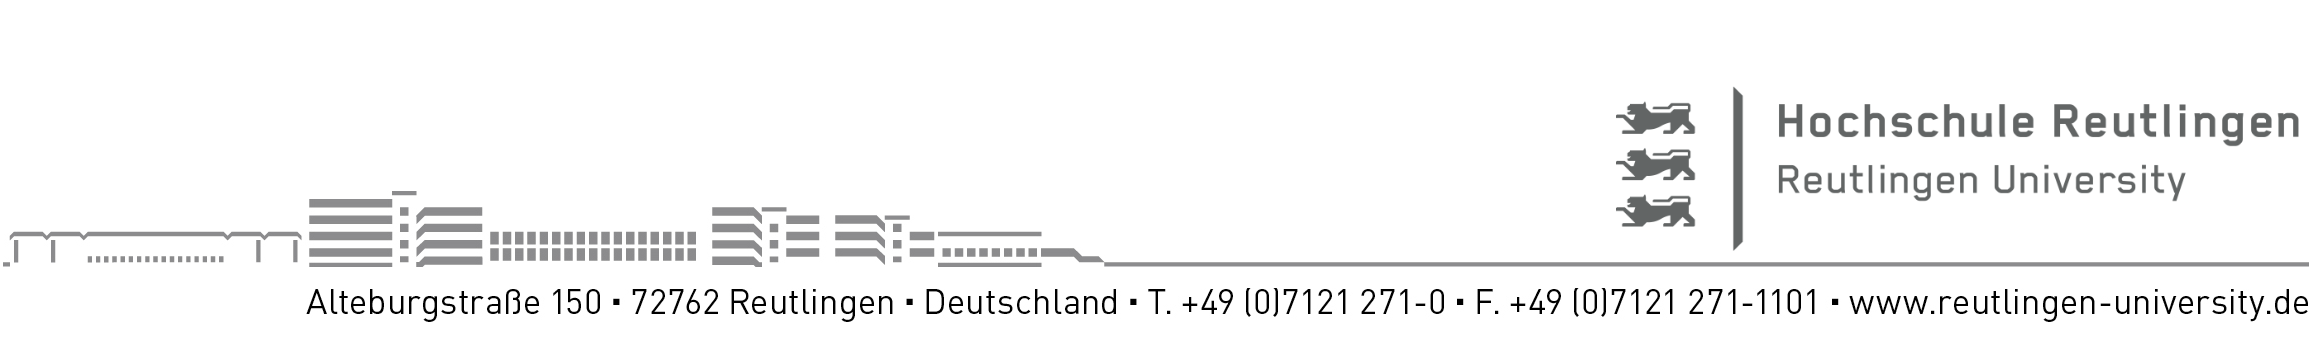
\includegraphics[width=1000pt,height=70pt,keepaspectratio]{images/FHRTFooter.png}
      \end{minipage}%
    }
  }
\end{titlepage}

\newpage
\selectlanguage{german}
\begin{abstract}
  Augmented Reality ist eine Technologie, die dem Nutzer ein visuelles 
  Erlebnis mit einer angereicherten Welt voller virtueller Objekte ermöglicht. Das Resultat, eine 
  Kombination aus Realität und Virtualität, bietet dem Benutzer eine neue Art der Wahrnehmung der Gegenwart. %Realitätswahrnehmung.  
  \\ 
  \linebreak
  Diese Bachelorarbeit befasst sich mit der Konzeption und Umsetzung eines industriellen Assistenzsystems unter Verwendung der Augmented Reality Technologie. Dabei soll die Umgebung 
  mit Hilfe des SLAM Verfahrens analysiert werden, um auf dieser Basis dreidimensionale Objekte als Referenz zu realen Objekten im Raum virtuell platzieren zu können. 
  Durch die entstehende Visualisierung können Informationen zu den jeweiligen Objekten in eine Datenbank eingetragen und angezeigt werden, dadurch kann das Überwachen von 
  Industriemaschinen vereinfacht werden. 
  \\ 
  \linebreak
  Zu dem Konzept gehört sowohl die Ausarbeitung der grundlegenden Softwarearchitektur, als auch ein allgemein-gültiges Datenmodell zur 
  Persistierung der generierten Daten. Für die bestmögliche Umsetzung der Augmented Reality Experience werden hierzu bereits schon bestehende Frameworks und Software 
  Development Kits, beispielsweise Google ARCore, verwendet. 
  \\ 
  Der entstandene Prototyp ist ein eigenständiges System. Die Architektur ist modular aufgebaut, um eine stetige Weiterentwicklung zu gewährleisten.  
\end{abstract}

\newpage
\selectlanguage{english}
\begin{abstract}
  Augmented Reality is a technology that enables the user to have a visual 
  experience with an enriched world full of virtual objects. The result offers the user a new 
  way of perceiving surrounding as an Combination of reality and virtuality.
  \\
  \linebreak
  This bachelor thesis deals with the conception and implementation of an industrial assistance system using augmented reality technology. The environment %should
  can be analyzed with the help of the SLAM method in order to be able to place three-dimensional objects virtually as a reference to real objects in space.
  The resulting visualization enables information on the respective objects to be entered in a database and displayed, which enables the simplified 
  monitoring of Industrial machines.
  \\
  \linebreak
  The concept includes the development of the basic software architecture as well as a generally applicable data model for
  saving the generated data. Already existing frameworks and software development kits where used for the best possible implementation of the 
  augmented reality experience as Google ARCore.
  \\
  The created prototype is an standalone system. The architecture is modular in order to ensure continuous further development.
\end{abstract}

\newpage
\selectlanguage{german}
\pagestyle{plain}
\chead{\headmark}
\cfoot{\pagemark}
%\pagestyle{headings}
\pagenumbering{Roman}
\tableofcontents           % Inhaltsverzeichnis hier ausgeben

\newpage
\pagenumbering{arabic}
\chapter{Einleitung}
\label{chap:Einleitung}
    Die folgende Master-Thesis befasst sich mit der Konzepterstellung einer zentralen Steuerzentrale, die 
    dem Entwickler die formalen Interaktionen, weitere Funktionen hinzuzufügen, erleichtern soll. Hierfür werden
    bereits bestehende Plattformen für \acl{SH} analysiert und daraus ein Konzept erstellt, die den Anforderungen 
    entsprechend einen größeren Mehrwert in der Weiterentwicklung der Plattform bietet. Die Umsetzung des ausgearbeiteten 
    Konzeptes wird nur in sehr geringem Maß behandelt.
    \\
    \linebreak
    In diesem Teil der Arbeit wird auf die Motivation des Themas eingegangen. Darüber hinaus 
    werden sowohl die Forschungsfragen als auch die Zielsetzung der Arbeit genauestens dargelegt. Darauf 
    folgend findet eine Übersicht über die Arbeit im Gesamten statt, mit der die Inhalte angerissen werden. 
    Eine nähere Betrachtung des Standes der Technik untermauert die Beweggründe dieser Themenwahl und 
    Ausarbeitung dessen. 

\section{Motivation}
\label{sec:Motivation}
    Jede neu entwickelte Technologie durchlebt im Laufe der Entstehung und Publikation ein enormes Aufsehen. 
    So lange bis diese Technik eine standardisierte Verwendung in der Gesellschaft findet oder sich als 
    unpraktikabel erweist und nicht weiter vorangetrieben oder eingestellt wird. Es wird in der Zeit des 
    Aufkommens und der Forschung viel darüber fantasiert, debattiert und geplant, ohne jedoch die Ausmaße und 
    Resultate der Forschungen und Praktiken abwägen zu können. Durch fehlende Erfahrung und nicht ausgereifte 
    Konzepte werden Höhepunkte und Illusionen erwartet, die zu diesem Zeitpunkt technisch nicht umsetzbar sind. 
    Um solche kühnen Versprechungen und Übertreibungen, sogenannte Hypes, die jede neue technologische Idee 
    mit sich bringt, von dem zu differenzieren was wirtschaftlich umsetzbar ist, werden bestimmte Phasen 
    der Entwicklung durchlaufen. \cite{gartner.2022m}
    \\
    \linebreak
    Die oben erwähnten Phasen der Entwicklung sind in einem sogenannten Hype-Zyklus, engl. Hype-Cycle, dargestellt. 
    Dieser Zyklus ist ein visualisiertes Modell, das die Entwicklung einer neuen Technologie von der Innovation 
    und Entstehung über die Forschung und Umsetzung bis hin zur ausgereiften Marktfähigkeit repräsentiert und so 
    diese Phasen der Entwicklung versinnbildlicht.  
    \\
    Entwickelt wurde der Hype Cycle von der Gartner Inc. Forschungsgruppe. Durch die Mitarbeiterin 
    Jackie Finn wurden die Definitionen der Entwicklungsphasen\footnote{Die Entwicklungsphasen der Gartner Inc. ist unter folgender URL zu finden: "\url{https://www.gartner.com/en/research/methodologies/gartner-hype-cycle}"} 
    geprägt. Diese sind wie folgt in fünf Phasen 
    dargestellt:
    \begin{enumerate}
        \item \textit{Innovationsauslöser, engl. Innovation Trigger}: Ein potentieller technologischer Durchbruch 
        löst die Dinge aus. Frühe Proof-of-Concept (PoC) Ansätze und ein großes Medieninteresse lösen eine 
        erhebliche Publizität aus. Oft gibt es keine brauchbaren Produkte und die Marktreife ist nicht 
        bewiesen. \cite{gartner.2022m}
        \item \textit{Höhepunkt überhöhter Erwartungen, engl. Peak of Inflated Expectations}: Frühe Publizität 
        bringt eine Reihe von Erfolgsgeschichten hervor – oft begleitet von zahlreichen Misserfolgen. 
        Einige Unternehmen ergreifen Maßnahmen; viele nicht. \cite{gartner.2022m}
        \item \textit{Trog der Ernüchterung, engl. Trough of Disillusionment}: Das Interesse schwindet, da 
        Experimente und Implementierungen nicht liefern. Hersteller der Technologie reißen es heraus 
        oder scheitern. Investitionen werden nur fortgesetzt, wenn die überlebenden Anbieter ihre Produkte 
        zur Zufriedenheit der frühzeitigen Anwender verbessern. \cite{gartner.2022m}
        \item \textit{Steigung der Erleuchtung, engl. Slope of Enlightenment}: Mehr Beispiele dafür, wie 
        die Technologie dem Unternehmen zugute kommen kann, beginnen sich zu herauszukristallisieren und 
        werden allgemeiner verstanden. Produkte der zweiten und dritten Generation erscheinen von den 
        Technologieanbietern. Mehr Unternehmen finanzieren Pilotprojekte; Konservative Unternehmen 
        bleiben vorsichtig. \cite{gartner.2022m}
        \item \textit{Plateau der Produktivität, engl. Plateau of Productivity}: Mainstream-Akzeptanz beginnt 
        sich abzuheben. Kriterien zur Bewertung der Lebensfähigkeit des Anbieters sind klarer definiert. 
        Die breite Markteinsetzbarkeit und Relevanz der Technologie zahlen sich eindeutig aus. \cite{gartner.2022m}
    \end{enumerate}
    Nachdem ein innovativer Gedanke den \textit{Höhepunkt überhöhter Erwartungen} passiert hat, z.B. die 
    Revolutionierung der Softwareentwicklung oder Szenarien, wie z.B. die Vollautomatisierung eines Gebäudes 
    oder Service-Roboter die uneingeschränkt interagieren können, die man in der Form nur aus Science-Fiction Filmen kennt, 
    folgt der \textit{Trog der Ernüchterung}. In Folge dessen wird festgestellt, dass die Erwartungen nicht 
    in Gänze übertragbar sind, bzw. nur zu einem geminderten Teil in die Realität umgesetzt werden können 
    und der verfolgte Gedanke an Interesse verliert. Nach erneutem Aufgriff der Technologie findet eine realistischere 
    Beurteilung der Innovation statt, die dazu beiträgt, dass die Technologie wieder an Interesse gewinnt. Die 
    objektive und realitätsnahe Betrachtungsweise formt ein neues und realistisches Bild der Potentiale, als auch 
    der Grenzen. Mit dem neu gewonnenen Maßstab geht die ehemals neue innovative Idee in eine routinierte Technologie über, 
    die an Anerkennung gewinnt und in der breiten Masse akzeptiert wird. Die Technologie erfährt mit steigender 
    Zuwendung eine stetigere Weiterentwicklung, die dann zu einer Community geformt wird. Mit der Erreichung dieses Status 
    befindet sich die Innovation, bezogen auf den Hype Cycle, in der letzten Phase, dem \textit{Plateau der Produktivität}, 
    und bestätigt so die Marktreife. Dieser Zeitpunkt löst die Zukunftsvision auf und es handelt sich um eine am Markt 
    etablierte Technologie.
    \\ 
    \linebreak
    Zum aktuellen Zeitpunkt befindet sich die Technologie rund um Plattformen für intelligente Geräte im privaten als auch im unternehmerischen 
    Bereich, engl. \textit{\ac{SH}} oder \textit{Connected Home}, im Anfangsstadium der letzten Phase, dem sogenannten 
    \textit{Plateau der Produktivität}. Mit zunehmender Akzeptanz werden im Umfeld des Internets der Dinge, engl. 
    \textit{\acl{IoT}}, stetig Szenarien entwickelt, die das Wachstum und die Verwendung von solchen Plattformen vorantreibt. 
    Mit einer immer tiefer gehenden Forschung und Umsetzung von Anwendungsbeispielen werden Bereiche offenbart, die 
    eine solche Plattform im privaten als auch im geschäftlichen Umfeld immer attraktiver gestaltet. Mit steigender  
    Konnektivität und Kompatibilität mehreren Geräten und Gegenständen können Szenarien und Prozessautomatisierungen, wie die 
    Steuerung von Service-Robotern, umgesetzt werden. Der jetzige technologische Fortschritt und die über die Forschungsjahre 
    gesammelten Erfahrungen bringt das Segment der intelligenten Geräte der \acs{IoT} den ursprünglich angedachten 
    Visionen und Ideen näher, sodass ein weiterer Ausbau dieser Technologie und dessen Anwendung stattfindet und sich 
    vollständig in den Markt etabliert. Der finale Schritt der endgültigen Marktreife ist ein faszinierender und wichtiger Grund 
    für meine Motivation, mich dieser Technologie und der dahinterstehenden Theorie zu widmen. Ein weiterer dazu beitragender Aspekt ist 
    die Steuerung und Verknüpfung von Geräten, sowie die Automatisierung von Prozessen innerhalb eines intelligenten Büros, um stetig hinzukommende 
    Anwendungsfälle abdecken und einfach implementieren zu können. Einen Ansatz zu schaffen, der einem Softwareentwickler eine Struktur vorgibt, die 
    in sich jedoch beliebig erweiterbar ist, sodass die Einschränkung von Prozessabbildungen minimiert wird. 
    % !!! Weiterer Grund zur Motivation: Dem Entwickler mehrere Freiheiten bei der Umsetzung von Anwendungsfällen oder Regeln zu 
    % !!! schaffen und die Regeldefinition nicht über ein Zusätzliches Framework abzubilden, sondern eine klar Struktur 
    % !!! vorzugeben, die klar definiert, welche grundlegenden Komponenten zu Erweiterung notwendig sind. Weitere Anpassungen oder 
    % !!! Anwendungsfälle verantwortet der Entwickler selbst. (Einbindung von APIs o.ä.)
    %
    %\\
    %Mit der erzielten Marktreife entstehen Produkte und Lösungen, die bestimme Teile der anfänglichen Idee abdecken. Mit 
    %zunehmender Entwicklung und anfallenden Anforderungen, werden viele Produkte zu groß und haben dadurch die grundlegende 
    %Konzeption und Architektur nicht vorausschauend entwickelt. Daher ist die anfängliche Überlegung und Konzeption essentiell.
    %\\
    %Daher ist ein weiterer Punkt meiner Motivation den Schritt zu gehen, ein Konzept zu entwickeln, dass die Erweiterung eines 
    %solchen Systems basierend auf der Konzeptgrundlage vereinfacht und so die Nutzung für Entwickler zur Weiterentwicklung verbessert.
    %
    % !!! Ein weiterer Punkt meiner Motivation ist die Vereinfachung der Erweiterung einer solchen Zentrale. 
    %Somit soll dem Entwickler bei einer stetigen Erweiterung der Plattform Zeit und Aufwand erleichtert werden. Dadurch können weitere 
    %Anwendungsszenarien und Objekte integriert werden, ohne einen zu großen Entwicklungsaufwand zu erzeugen.   
    \\ 
    \linebreak
    Die Einsatzgebiete von intelligenten Geräten, beziehungsweise die Verwendung von Kompaktlösungen, Plattformen und Steuereinheiten zielen räumlich 
    auf Gebäude, Häuser und Wohnungen ab und bieten viele Verwendungs- und Einsatzmöglichkeiten, die stetig ausgebaut und optimiert werden. 
    Diese sehen wie folgt aus: 
    \begin{itemize}
        \item Komfort
        \item Entertainment
        \item Überwachung und Sicherheit
        \item Steuerung von Prozessen
        \item Management von Automatisierungen (Automationen)
    \end{itemize}    
    Neben der Affinität von \acl{SH} zum \acl{IdD} und der damit einhergehenden Technologie bringt diese Vorteile mit sich, wie z.B. 
    die Modernisierung von Wohn- und Bürogebäuden und die routinierte Ausführung und Abarbeitung von Prozessen, die dem Menschen 
    Aufgaben und Arbeiten abnehmen.
\pagebreak
\section{Forschungsfragen}
\label{sec:forschungsfragen}
    Die in der Arbeit zentral behandelte Forschungsfrage ist wie folgt definiert: 
    \\
    \linebreak
    \textit{F1: Wie kann man die Usability von Prozessautomatisierungen und Regeldefinitionen von SmartHome-Plattformen optimieren, sodass die formalen Interaktionen der Softwareentwickler schneller sind?}
    \\
    \linebreak
    Eine Konkretisierung identifiziert konkret die Herausforderungen existierender Plattformen in Bezug auf die Definition von Regeln und Automatisierungen:
    \\
    \linebreak
    \textit{F1.1: Welche sind die Usability-Herausforderungen existierender Plattformen, bzw. welche Anforderungen würden für eine Optimierung gelten?}
    %-	Wie kann man die Usability von Prozessautomatisierungen und Regeldefinitionen von SmartHome-Plattformen optimieren, so dass die formalen Interaktionen der Softwareentwickler schneller sind?
        %o	Welche sind die Usability-Probleme der existierenden Plattformen? 
        %o	Welche Anforderungen würden für eine Verbesserung einer solchen Plattform gelten?
        % Nicht Bestandteil der eigentlichen Forschungsfrage: 
        % -Reicht eine Kommunikationsschnittstelle als Ausgangspunkt für alle Verbindungen?

    % - Wie kann man die Usability von Smart Home - Plattformen optimieren, sodass die formalen Interaktionen der Softwareentwickler schneller sind? 
    %  - Wie kann ein Framework vorgegeben werden, dass den Entwickler (Anwender) bei der Implementierung von Regeln (und der Erweiterung um 
    %    anwenderbasierte Funktionalitäten) nicht einschränkt?

\section{Zielsetzung der Arbeit}
\label{sec:zielsetzung}
    %TBD Wird zum Schluss geschrieben. 
    %Programmierseitige Möglichkeit um Regeln umzusetzen.
    Das Ziel der Arbeit ist die Erarbeitung eines Konzeptes und die prototypische Implementierung des Frameworks, welches dem Softwareentwickler das 
    Umsetzen von Regeln und zu automatisierende Prozesse im Rahmen der Programmierung erleichtert und in der Ausprägung 
    der Regeln nicht einschränkt. Dabei wird sich an bestehenden Produkten orientiert, die versuchen, diese 
    Automatisierungen für den Nutzer vereinfacht darzustellen. Die aktuellen Praktiken setzen trotz dessen eine starke Lernkurve voraus. 
    %und lässt den Nutzer Regeln und Prozesse nur beschränkt einfach abbilden. 
    Mit dem Framework soll dem Anwender eine Struktur an die Hand gegeben werden, mit der Regeln und Prozesse innerhalb eines 
    smarten Büros einfach abgebildet werden können. Die Abarbeitung von Regeln und Prozessen sollen über das Framework 
    koordiniert werden, sodass der Anwender sich ausschließlich um die Regeldefinition und um die abzubildende Umgebung durch Geräte, Zustände und weitere 
    potentielle Mittel innerhalb eines smarten Büros, kümmern muss. 
    %"Anleitung" dem Entwickler an die Hand zu geben, dass Prozesse schnell umgesetzt werden können und jedoch 
    % keinerlei Einschränkungen hat, da mit Java (Spring Boot) keine Grenzen gesetzt sind und mit dem Framework auch 
    %keine Grenzen gesetzt werden.

    %%%%%%%%%%%%%%%%%%%%%%%%%%%%%%%%%%%%%%%%%%%%%%%%%%%%%%%%%%%%%

    % ZIEL DES KONZEPTES: Ein Framework für Entwickler bereitzustellen, welches die Mächtigkeit für den Entwickler offen lässt, nicht einschränkt 
    % und dennoch Konfiguration und Ausführung umsetzt. Der Entwickler muss lediglich den Zustandsraum, die MQTT-Topics und die Regeln definieren.
    % Der Entwickler bekommt ein Framework in die Hand, welches die Umsetzung von Prozessen in einem smarten Büro ermöglicht. Das Framework kümmert sich um die 
    % Organisation und die Ausführung der Regeln. Die Richtigkeit der Regeln und des Zustandsraumes muss der Entwickler sicherstellen. 
    % Die Kommunikation über MQTT ist nur eine Möglichkeit. Des Setup wird wegabstrahiert 


    %%%%%%%%%%%%%%%%%%%%%%%%%%%%%%%%%%%%%%%%%%%%%%%%%%%%%%%%%%%%%

\section{Forschungsstrategie und Forschungsmethoden}
\label{sec:forschungsstrategie}
    Dieser Abschnitt der Arbeit widmet sich der Forschungsstrategien und der darauf angewendeten Forschungsmethoden. 
    Hierbei werden die Strategien kurz erläutert und die Methoden skizziert. Die Anwendung der Strategien findet zu 
    späterem Zeitpunkt statt. 
    \\
    Diese Arbeit ist in die drei Phasen aufgeteilt, Forschung, Konzeption und Evaluation. Zuerst erfolgt durch ein 
    systematisches Literaturreview eine Analyse des aktuellen Stands der Technik, welche die Forschungsfragen aufgreift und 
    anhand dessen den aktuellen Stand identifiziert. Schwerpunkt dabei liegt auf der einfachen Handhabung der formalisierten 
    Interaktionen eines Softwareentwicklers bei der Weiterentwicklung, bzw. bei der Ergänzung einer bestehenden 
    Softwarelösung, um weitere Anwendungsfälle abzudecken. 
    In der Phase der Anforderungserhebung werden Experteninterviews durchgeführt, mit denen die Anforderungen des Produktes, 
    für welches ein Konzept erstellt wird, identifiziert werden. Ergänzend dazu werden im Rahmen der Arbeit weitere 
    Anforderungen durch das \ac{RE} und der Anwendung des \textit{user-centered design}-Prinzips\footnote{Iterativer Prozess zur Ermittlung von Anforderungen, die nutzerorientiert aufgestellt werden. \url{https://www.interaction-design.org/literature/topics/user-centered-design} Abgerufen am 08.05.2022} 
    sowie des \textit{target group analysis}-Ansatzes (\ref{sec:zielgruppenanalyse}) ermittelt. Dabei wird die 
    Nutzerorientierung auf den Softwareentwickler ausgelegt. 
    Zur anschließenden Evaluation wird ein Usability Test durchgeführt und darauf erneut ein Experten Interview, damit 
    Eindrücke über das Konzept entstehen und die Erfahrungen der Experten während des Usability Tests 
    in die Beantwortung der Forschungsfrage mit einfließen.
    \\
    Die soeben genannten Forschungsmethoden werden im Nachfolgen- den näher erklärt.

    \subsection{Experteninterview}
    \label{subsec:experteninterview}
        Zu Anfang wird bei einem Experten Interview der Hintergrund des Interviews erläutert. Nachdem die interviewende 
        Person den Grund dargelegt hat, stellt ein Forscher einem Experten ausgewählte Interview-Fragen, die für die 
        Forschung relevant sind und dazu beitragen die Forschungsfrage zu beantworten.
        \\
        \linebreak
        Die Interview-Fragen können als offene oder geschlossene Fragen formuliert werden, je nachdem ist eine beliebige Reihe 
        an Antworten möglich oder nur eine begrenzte Anzahl an Antworten \cite{robson2002real}. Der Verlauf des Interviews 
        kann von dem Forscher selbst bestimmt werden. Sind nur bestimmte Antworten gewünscht, so können die Fragen strukturiert und 
        geschlossen formuliert werden. Ebenso gibt es den semi-strukturierten und den unstrukturierten Ansatz, bei dem das Interview 
        offen gestaltet werden kann. Der Semi-Strukturierte Ansatz eignet sich, wenn spezielle Fragen adressiert werden, bzw. eine 
        Reihenfolge festgelegt ist, sodass der Interviewer eine klare Reihenfolge hat. Mit dem unstrukturierten Vorgehen wird 
        ein völlig offenes Interview angestrebt, bei dem der Verlauf abhängig von dem Inhalt der Konversation ist.

    \subsection{Systematisches Literaturreview}
    \label{subsec:systematischesliteraturreview}
        Mit einem systematischen Literaturreview wird zur evidenzbasierten Identifizierung, Bewertung und Interpretation  
        von bestehender Literatur eine wissenschaftliche Methode angewendet, mit der Fragestellungen zu einer bestimmten Thematik 
        herausgearbeitet werden können. Mithilfe diesen Ansatzes soll die Erzielung einer Schlussfolgerung zu einem untersuchten Objekt 
        ermöglicht werden. 
        Die Methodik des systematischen Literaturreviews orientiert sich an den Richtlinen von Kitchenham et al.. Diese ist in drei 
        aufeinander aufbauende Schritte gegliedert. Zu Beginn erfolgt die Planung, anschließend die Durchführung und abschließend die 
        Dokumentation und Offenlegung der Ergebnisse \cite{Kitchenham2007}.

    \subsection{Usability-Test}
    \label{subsec:usabilitytests}
        Ein Usability-Test ist eine Methode zur Testung von Prototypen oder Arbeitsversionen von Computerschnittstellen \cite{LAZAR2017263}. 
        Das Testen der Nutzbarkeit kann durch vorab definierte Aufgaben, die durch Probanden und Benutzer in einer dafür vorgesehenen 
        Umgebung durchgeführt werden, erfolgen. Die Aufgaben können je nach Anwendungsfeld oder -kontext unterschiedlich ausfallen. 
        Ebenso können solche Tests auch dazu beitragen, um physische Interaktionen mit bspw. Geräten zu bewerten. 
        \\
        Alle Ansätze für Usability-Tests haben ein grundlegendes Ziel: Die Qualität einer Schnittstelle zu verbessern und den 
        dafür vorgesehenen Anwendern diese Benutzung so einfach wie möglich zu gestalten \cite{LAZAR2017263}. Während diese Tests optimaler 
        Weise Schnittstellenfehler aufdecken, die den Benutzern Schwierigkeiten bereiten, ist gleichzeitig rauszufinden, welches Schnittstellendesign 
        gut funktioniert, um dieses für Zukünftige Entwicklungen beizubehalten. 
        \\
        \linebreak
        Zur Kategorisierung von durchgeführten Tests, werden Werkzeuge verwendet, die das Verhalten und die Meinungen der Benutzer 
        messbar macht. Eines dieser Werzeuge ist das \textit{System Usability Scale (SUS)}\footnote{System Usability Scale. \url{https://www.usability.gov/how-to-and-tools/methods/system-usability-scale.html} Besucht am 03.07.2022}. 
        Dabei handelt es sich um einen einfachen 
        technologieunabhängigen Fragebogen, anhand dessen die Gebrauchstauglichkeit eines Systems bewertet werden kann. Dieser 
        ist eine Praktik zur quantitativen Analyse der Nutzbarkeit. Der Umfang umfasst zehn Fragen nach der Likert-Skala \cite{likert1932technique}.

\section{Aufbau der Arbeit}
\label{sec:aufbau}
    Die vorliegende Master-Thesis gliedert sich nach den soeben genannten einleitenden Information im Aufbau in insgesamt 
    zehn Kapitel. Das erste Kapitel (\ref{chap:Einleitung}) beschreibt die Motivation (\ref{sec:Motivation}), welche die 
    Intension kundtut, diese Thematik rund um \acs{IoT} und Smart Home zu bearbeiten. Darauf folgend werden die 
    Forschungsfragen (\ref{sec:forschungsfragen}), die im Rahmen der Thesis behandelt werden, erläutert. Nach der 
    Beschreibung der Forschungsfragen wird im anknüpfenden Abschnitt (\ref{sec:zielsetzung}) die Zielsetzung der 
    Arbeit erläutert. Hierbei werden zusätzliche Schwerpunkte und Ziele aufgegriffen. Abschließend wird das Unternehmen, in der 
    die Thesis geschrieben wird, hervorgehoben und deren Absichten in Verbindung mit Innovationen beleuchtet. 
    \\
    \linebreak
    Das Kapitel (\ref{chap:grundlagen}) widmet sich den essentiellen und wichtigen Grundlagen dieser Arbeit. Zu Anfang wird dem 
    Leser der Terminus des \acl{IoT} (\ref{sec:iot}) offenbart, um zum Teil den Kontext im Bezug zu dieser Arbeit zu begreifen, 
    gefolgt von einer Einführung in die Thematik des \acl{SH} (\ref{sec:smartHome}), der Problematik der Begriffsdefinition, der 
    historischen und kontinuierlichen Entwicklung und mit den Zielen, die mit der Verwendung einer Smart Home Lösung bewältigt 
    werden sollen. Mit dem Verständnis der übergeordneten Begriffe, \acs{IoT} und \acl{SH}, werden Technologien 
    (\ref{sec:technologien}) aufgegriffen, die im Rahmen dieser Arbeit erwähnenswert sind und verwendet werden. %Um auf die Vielfältigkeit 
    %von der Umsetzung eines \acl{SH} einzugehen und einen Teilaspekt der Anforderungen Abzudecken, wird ebenso auf Service-Roboter 
    %(\ref{sec:roboter}) eingegangen. 
    Abschließend werden in Kapitel (\ref{chap:grundlagen}) die Softwarelösungen, Home Assistant 
    und openHAB (\ref{sec:homeassistant} \& \ref{sec:openhab}), dargestellt. Diese dienen zur Grundlage für die Evaluation als 
    auch zur Gegenüberstellung der Lösungen in Kapitel (\ref{chap:evaluation}) Diskussion und Evaluation. 
    \\
    \linebreak
    Die theoretischen und methodischen Hintergründe sowie den Stand der Technik wird in Kapitel (\ref{chap:technikStand} )
    angesprochen. Dieser Teil enthält Beschreibungen, Forschungen und aktuelle Erkenntnisse über Technologien, die im Umfeld der 
    Smart Home Anwendungen innerhalb des \acs{IoT} verwendet werden. Zudem werden in Zusammenhang der Erkenntnisse und 
    Möglichkeiten der Technologie die Szenarien dargestellt. 
    \\
    \linebreak
    Kapitel (\ref{chap:anforderungsanalyse}) befasst sich mit den Anforderungen, engl. Requirements, die für die 
    eigentliche Konzeption relevant sind. Innerhalb dieses Kapitels wird anhand von Informationen und den umzusetzenden 
    Szenarien die Anforderungen für die Konzeption erarbeitet. Hierbei werden aus der Praxis bekannte Verfahren verwenden, um 
    die Anforderungen zu definieren. Mittels den zugrundeliegenden Anforderungen wird im nachfolgenden Schritt die eigentliche 
    Konzeption dargelegt.
    \\
    \linebreak 
    Nach Aufbereitung der Anforderungen durch das sogenannte Anforderungsmanagement, engl. \textit{Requirements Engineering},
    wird in Kapitel (\ref{chap:konzept}) das Konzept erarbeitet, welches als Grundlage für die prototypische Implementierung und 
    Umsetzung des Konzepts dient. Das Konzept befasst sich mit den Anforderungen und setzt diese ein, um die Organisation des 
    Systems in Komponenten, deren Beziehungen zueinander und zur Umgebung sowie deren Prinzipien zu definieren. Zum Ende des 
    Konzepts steht eine Architektur, die sich aus den Anforderungen und auch aus den Analysen der eigentlichen Forschungsfrage 
    abzeichnet.
    \\
    \linebreak
    In Kapitel (\ref{chap:umsetzung}) wird die Umsetzung des Konzepts skizziert. Darunter welche Problem während der Implementierung 
    auftraten als auch deren Lösungsfindung. Ebenso wird hier aus praktischer Sicht auf die Architektur geschaut, welche Komponenten,  
    Bibliotheken und zusätzliche Systeme, engl. \textit{Frameworks}, verwendet wurden. Das erzielte Ergebnis und Resultat wird 
    abschließend zusammengefasst und neutral betrachtet.
    %\\ 
    %\linebreak
    %Das Ergebnis wird aus objektiver Sicht in dem darauf folgenden Kapitel (\ref{chap:ergebnis}) erläutert. 
    \\
    \linebreak
    Nach Abschluss der Umsetzung und dessen Ergebnisdokumentation befasst sich das Kapitel (\ref{chap:evaluation}) mit der Diskussion 
    und Evaluation. Hier findet eine Analyse des Konzepts sowie deren Umsetzung und objektive Betrachtung statt. Anschließend werden 
    Vergleiche zwischen der Eigenentwicklung und bereits bestehender Softwarelösungen, die im Grundlagenkapitel aufgefasst werden, 
    aufgestellt und bewertet. %Testdurchführung und anschließende Evaluation (Experten Interview)
    \\
    \linebreak
    Im vorletzten Teil, Kapitel (\ref{chap:fazit}), wird ein Fazit aus den Erkenntnissen und Ergebnissen gezogen. Dieses Schlussresümee 
    führt nochmals die Höhepunkte sowie eine eigene Einschätzung auf. 
    \\
    \linebreak
    Zum Abschluss der Thesis wird in Kapitel (\ref{chap:ausblick}) ein Ausblick gegeben. Dieser gibt Aufschluss darüber, welche 
    Erweiterungsmöglichkeiten es für die in dieser Thesis erfolgten Arbeit gibt und wie innovativ sich dieser Grundbaustein in Zukunft 
    erweisen könnte. 

%\section{CGI}
%\label{sec:cgi}
%\section{Forschungsfragen}
Hallo
%\section{Zielsetzung der Arbeit}
Zielsetzung / Zielerreichung
%\section{Aufbau der Arbeit}
Hallo Test
\chapter{Grundlagen}
\label{chap:grundlagen}
    In diesem Kapitel werden die für diese Thesis relevanten Grundlagen geschaffen, um ein Grundverständnis und 
    fundiertes Wissen über verwendete Technologien zu erlangen und die nachfolgende Recherche, Konzeption und 
    Umsetzung besser verstehen zu können. 

    % Beschreibung
    % Definition
    % Gesamtbild 
    % Historische Entwicklung 

\section{Internet der Dinge}
\label{sec:iot}
    Das \ac{IdD}, im Englischen \ac{IoT}, zählt als eines der Schlagworte in der \ac{IT}. In der Domäne des \acs{IoT} bekommen 
    Gegenstände und Objekte eine eindeutige Identität, die eine Kommunikation miteinander als auch das Entgegennehmen von 
    Befehlen erlaubt. Mit dem \acl{IdD} lassen sich Anwendungen sowie Prozesse automatisieren und Aufgaben erledigen ohne das 
    von außen Eingegriffen werden muss \cite{bigdatainsider2016}. Die Prozessautomatisierung findet sich auch im Kontext des 
    \acl{SH} wieder, welches in nachfolgendem Kapitel genauer aufgegriffen wird. 
    \\
    \linebreak
    In der einschlägigen Literatur gibt es für das \acl{IoT} keine allgemeingültige Definition die alle Anwendungsbereiche abdeckt. 
    Die Definitionen und Auslegungen der Interpretation unterscheiden sich je nach Anwendungsgebiet. Demnach gibt es viele verschiedene 
    Forschungsgruppen, darunter Forscher, Akademiker, Innovatoren, Entwickler und Geschäftsleute, die den Begriff oder die zugrundeliegende 
    Problemstellung definiert haben. Die Ursprünge jedoch sind dem Experten für digitale Innovationen, Kevin Ashton\footnote{Britischer Technologie-Pionier, Mitgründer des Auto-ID Centers am Massachusetts Institute of Technology (MIT). \url{https://de.wikipedia.org/wiki/Kevin_Ashton} (Abgerufen am 22.03.2022)}, 
    zuzuschreiben. 
    \\ 
    Die in der Literatur auffindbaren Definitionen verfolgen zwei Sichtweisen, zum Einen aus Sicht des aktiven, dass die Daten von 
    Menschen erstellt wurde, zum Andere, aus Sicht des passiven, dass die Daten von Dingen, darunter die Sensoren und Aktoren, 
    erstellt wurde. \cite{Madakam2015} Eine aus dem Zusammenschluss hervorgehende Definition ist, dem wissenschaftlichen Artikel zufolge, folgende:
    % „Ein offenes und umfassendes Netzwerk intelligenter Objekte, die in der Lage sind, sich automatisch zu organisieren, 
    % Informationen, Daten und Ressourcen auszutauschen und auf Situationen und Veränderungen in der Umgebung zu reagieren 
    % und zu handeln.“
    \pagebreak
    \begin{quote}
        “An open and comprehensive network of intelligent objects that have the capacity to auto-organize, share information, data 
        and resources, reacting and acting in face of situations and changes in the environment” \cite{Madakam2015}
    \end{quote}
    Daraus kann abgeleitet werden, dass der Begriff des \acl{IdD} für die Vernetzung von Gegenständen im privaten Gebrauch oder 
    von Geräten und Maschinen im industriellen Umfeld über das Internet steht. Damit Geräte individuell angesprochen werden können, werden diese 
    mit einer eindeutigen Identität, genauer einer \ac{IP}-Adresse, im Netzwerk belegt und mit elektronischer Intelligenz ausgestattet \cite{bigdatainsider2016}.
    Darüber sind die Netzwerkteilnehmer im Stande, über das Internet zu kommunizieren Prozesse automatisiert zu erledigen. Die sogenannten 
    \textit{intelligenten Geräte} werden auch oft mit dem englischen Begriff, \textit{Smart Devices}, betitelt. 
    \\
    \linebreak
    Neben der Kommunikation der Geräte über das Netzwerk untereinander kann ebenso entweder durch das Gerät selbst oder eine zentrale 
    Schnittstelle über das Internet interagiert werden. Dadurch sind Objekte und Gegenstände durch einen Benutzer von beliebigen Orten 
    auch außerhalb des Netzwerks erreichbar und können so bedient werden. Diese Art und Weise wird auch in dem zentralen Thema des 
    \acl{SH} verwendet. Die Funktion als auch die Umsetzung wird im Kapitel (\ref{sec:smartHome}) näher beleuchtet.
    \\
    \linebreak
    Das \acl{IdD} ist ein nahezu existenzielles Konzept der \acs{IT}-Welt. Mit dem \acs{IoT} wird die Vision verfolgt eine globale 
    Infrastruktur zu erstellen, mit dem physische Objekte miteinander vernetzt werden und jeder Zeit zur Verfügung stehen. Das \acl{IoT} 
    kann auch als globales Netzwerk angesehen werden, indem die Kommunikation zwischen Mensch zu Mensch, Gerät zu Mensch und Gerät zu 
    Gerät ermöglicht. In vielen Artikeln wird auch davon gesprochen, dass mit der Technologie die Verschmelzung der digitalen und 
    der physischen Welt vorangetrieben wird.\footnote{Das Internet der Dinge – der digitale Zwilling der Welt. Kompetenzzentrum Öffentliche IT in Kooperation mit dem Fraunhofer Institut. \url{https://www.oeffentliche-it.de/trendsonar-iot} Abgerufen am 23.03.2022.} 
    Die Vereinigung beider Welten ist die Verknüpfung physischer Objekte, die eindeutig identifizierbar sind, mit einer virtuellen 
    Repräsentation in einer vergleichbaren Internet-Struktur. 

    \subsection*{Gesamtbild des \acl{IoT}}
        Der folgenden Abbildung (\ref{pic:mindmap_IoT}) ist zu entnehmen, welche Technologien rund um das \acl{IdD} liegen und in Verbindung damit stehen. 
        \begin{figure}[hbt!]
            \centering
            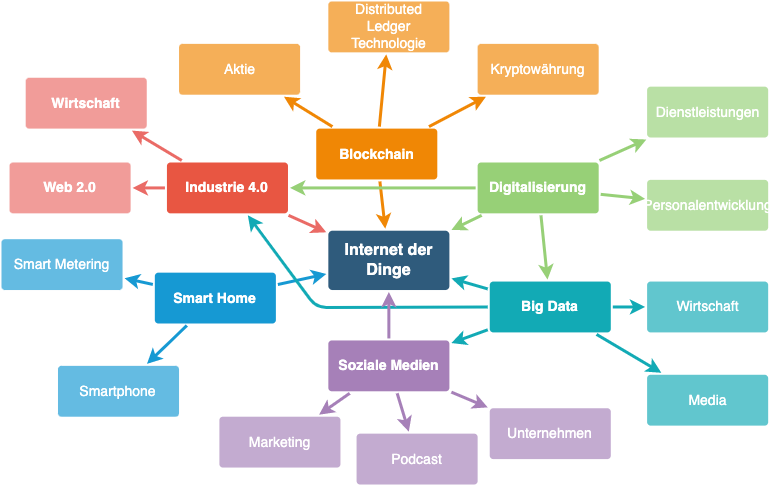
\includegraphics[width=13cm,height=13cm,keepaspectratio]{images/IoT-Mind_Map.png}
            \caption{Technologische Einordnung von IoT \cite{iotmindmap2018}}
            \label{pic:mindmap_IoT}
        \end{figure}
        \\
        \pagebreak
        Beispielsweise ist das \acs{IoT} eine wesentliche Grundlage für das Themengebiet \textit{Big Data}. Die durch Sensoren und Aktoren erzeugten Daten 
        können Grundlage für die Verwendung im Bereich \textit{Big Data} sein. Dabei werden die Datenmengen gespeichert und mithilfe von Mustern 
        und Herangehensweisen des Big Data analysiert. 

    \subsubsection*{Anwendungsbereiche des \acs{IoT}}
        Grundlegend können im Bereich des \acl{IoT} zwischen zwei Anwendungsbereichen unterschieden werden, zum Einen im privaten Bereich und zum 
        Anderen im industriellen Bereich. %Einsteuerung von IIoT% 

        %Grundsätzlich kann beim Internet der Dinge zwischen privaten und industriellen Anwendungen unterschieden werden. Im privaten Umfeld sind 
        %hauptsächlich Gegenstände des alltäglichen Gebrauchs für eine komfortablere und intelligentere Nutzung untereinander vernetzt. Es lassen 
        %sich beispielsweise intelligente Gebäudeautomatisierungen installieren oder Geräte realisieren, die bei bestimmten Ereignissen per Internet 
        %mit dem Anwender in Kontakt treten.
    
        %Im industriellen Bereich geht es hauptsächlich darum, Maschinen und Anlagen so miteinander zu verbinden, dass sich ganze Industrieprozesse 
        %automatisieren lassen. Produktionsabläufe werden dadurch effizienter und günstiger. Das Internet der Dinge ist eine elementare Komponente 
        %der so genannten Industrie 4.0. Mit dem IoT und Industrie 4.0 wird die Selbstorganisation von industriellen Prozessen durch die direkte 
        %Kommunikation von Maschinen, Anlagen, Waren und Menschen möglich. Es lassen sich nicht mehr nur einzelne Produktionsschritte, sondern 
        %ganze Wertschöpfungsketten automatisieren und wesentlich effizienter gestalten.




    %\subsection{IIoT}

\subsection{Edge und Cloud Computing}
    %Definition Edge Computing
    %Definition Cloud Computing
    % Unterschiede der beiden Ansätze und in Zusammenhang mit IoT (kurz)

\subsection{Ziele von \acs{IoT}}
%\section{Smart Home}
\label{sec:smartHome}
    \acl{SH}, übersetzt in Deutsch \textit{“intelligentes Zuhause“}, ist einer von mehreren bekannten Zweigen des \acs{IoT}s. 
    Speziell diese Rubrik widmet sich explizit 
    sämtlichen Haushaltsgeräten und -einrichtungen. Aus diesem Grund können viele Geräte ebenso intelligente Gegenstände 
    der Rubrik \acl{SH} sein. Ein kleiner Ausschnitt solcher Nutzgegenstände sind unter anderem Lampe, Kontaktsensoren, 
    Thermostate, Service-Roboter, Staubsauger-Roboter, Kühlschränke Geräte rundum die Haussicherheit. 
    \\ 
    Unter dem Oberbegriff \acl{SH} ist auch eine Weise zu verstehen, mit der die Erhöhung der Wohn- und Lebensqualität, 
    effizienteren Energienutzung unter Verwendung vernetzter und fernsteuerbarer Geräten, Sicherheit sowie automatisierbaren 
    Abläufe gesteigert werden kann. 
    \\ 
    Der Begriff intelligenten Zuhause wird auch schon verwendet, wenn die Haustechnik und Haushaltsgeräte unter einander  
    vernetzt sind. Die Definition im Deutschen Gebrauch, welche nach (Strese et al. 2010) in der Untersuchung im Rahmen 
    der wissenschaftlichen Begleitung zum Programm Next Generation Media (NGM) des Bundesministeriums für Wirtschaft und 
    Technologie aufgegriffen wird, lautet wie folgt: 
    \begin{quote}
        „Das Smart Home ist ein privat genutztes Heim (z.B. Eigenheim, Mietwohnung), in dem die zahlreichen Geräte der 
        Hausautomation (wie Heizung, Beleuchtung, Belüftung), Haushaltstechnik (wie z.B. Kühlschrank, Waschmaschine), 
        Konsumelektronik und Kommunikationseinrichtungen zu intelligenten Gegenständen werden, die sich an den 
        Bedürfnissen der Bewohner orientieren. Durch Vernetzung dieser Gegenstände untereinander können neue 
        Assistenzfunktionen und Dienste zum Nutzen des Bewohners bereitgestellt werden und einen Mehrwert 
        generieren, der über den einzelnen Nutzen der im Haus vorhandenen Anwendungen hinausgeht.“ \cite{strese.2010m}
    \end{quote}
    Eine vergleichbare Definition wurde zu späterem Zeitpunkt durch eine Literaturrecherche publiziert. Diese beschreibt 
    die zugrundeliegende Thematik weniger aus Anwendersicht sonder widmet sich vielmehr dem System und der Konnektivität. 
    \begin{quote}
        „A smart home is a place with heterogeneous systems to many
        front devices with the support of embedded information and
        communication architectures[...]“ \cite{Balakrishnan2018}
    \end{quote}
    Den beiden Definitionen ist zu entnehmen, dass die Kernaussage eine ähnliche ist, es jedoch in Büchern, Fachartikeln, 
    Publikationen an Universitäten und in den verbreiteten Medien bis heute keine durchgängige Definition gibt. Aus der 
    empirischen Literatur wird ersichtlich, dass viele Synonyme für die Benennung der Thematik verwendet werden, darunter 
    beispielsweise: \cite{strese.2010m}
    \begin{itemize}
        \item Connected Home
        \item Elektronisches Haus
        \item Intelligentes Haus (engl. Smart House)
        \item Smart Living
        \item Home of the Future 
    \end{itemize}
    
\section{Technologien}
\label{sec:technologien}
    Die bereits angesprochene Kommunikation und Vernetzung zwischen Geräten basiert im Allgemeinen auf 
    diversen Protokollen. Um diese Datenbewegung und Kommunikation besser verstehen zu können, werden im 
    Folgenden bekannte Protokolle erwähnt und aufgeführt und eines der meist verwendeten näher betrachtet. 
    Um einen Vergleich herzustellen, wird ein vergleichbares Protokoll betrachtet. Diese werden dann zum 
    Abschluss gegenübergestellt. 

    \subsection{Übertragungsmethoden}
    \label{subsec:netzwerkprotokolle}
    Allgemein gibt es im Bereich des \acl{SH} mehrere Methoden und Möglichkeiten, die Objekte miteinander zu vernetzen. 
    Unter dessen gehören Protokolle über Bluetooth, Ethernet, WLAN, Bussysteme, Funk und Stromleitung. 
    Diese werden Abhängig von den Herstellern eingesetzt. Proprietäre Systeme funktionieren nur über eine 
    Übertragungsmethode. So erzwingen die Hersteller die Nutzung einer Produktlinie, bzw. den Kauf einer 
    einheitlichen Lösung. Geräte die die Möglichkeiten besitzen über mehrere Protokolle 
    zu kommunizieren sind flexibler einsetzbar und mit mehreren Plattformen und Geräten kompatibel.
    Grundlegend werden mit diesen Übertragungsmethoden Netzwerke erstellt, über das die Geräte in einem \acl{SH} kommunizieren können.
    Die populärsten werden in folgender Tabelle aufgelistet: 
    \begin{table}[hbt!]
        \begin{center}
            \begin{tabular}{| p{3.25cm} | p{3.25cm} | p{3.25cm} | p{3.25cm} |}
                \hline
                    \textbf{Technologie} & \textbf{Übertragung} & \textbf{Frequenzbereich (Funk)} & \textbf{Proprietär} \\
                \hline
                    ZigBee & Funk & 2,4 GHz, 868 MHz & Nein \\ 
                \hline
                    Z-Wave & Funk & 868 MHz & Nein \\ 
                \hline
                    HomeMatic & Funk / Datenleitung & 868,3 MHz & Ja \\
                \hline
                    KNX & Funk / Strom- und Datenleitung & 868 MHz / - & Nein / Ja (Datenleitung als Gesamtsystem) \\
                \hline
                    Wi-Fi / WLAN & Funk & 2,4 - 5 GHz & Nein \\
                \hline 
                    Bluetooth & Funk & 2,4 GHz & Nein \\
                \hline
                    io-homecontrol & Funk & 868-870 MHz & Ja \\
                \hline
            \end{tabular}
        \end{center}
        \caption{Übertragungsmethoden des Smart Home}
        \label{tab:protocolsSH}
    \end{table}
    \\
    Die Auflistung der zum aktuellen Zeitpunkt am meist verwendeten Übertragungsmethoden dient 
    lediglich als Einblick, damit eine große Gesamtübersicht der Technologien und der Thematik \acl{SH} entsteht. 
    Demnach wird im Rahmen dieser Arbeit das Thema oberflächlich erläutert und nicht ausführlich vertieft.
    %ZigBee? Erläuterung etwas detaillierter?

    % https://www.bigdata-insider.de/so-laeuft-der-datenaustausch-zwischen-edge-und-cloud-a-1097887/ 

    \subsection{MQTT}
    \label{subsec:mqtt}
        Das \ac{MQTT}-Protokoll ist eines der ältesten offenen Netzwerk- und Nachrichtenprotokolle der 
        \ac{MtoM}-Kommunikation. 
        Dies wurde 1999 von IBM Mitarbeiter Andy Stanford-Clark\footnote{Informationen zu Herrn Stanford-Clark \url{https://stanford-clark.com} Abgerufen am 12.04.2022} 
        und von Cirrus Link Solutions Mitarbeiter Arlen Nipper\footnote{Informationen zu Herrn Nipper \url{https://www.inductiveautomation.com/resources/podcast/the-coinventor-of-mqtt-arlen-nipper-from-cirrus-link-solutions} Abgerufen am 12.04.2022} 
        entwickelt. Die Technologie ermöglicht die Übertragung von Messdaten, sogenannten Telemetriedaten, in Form von 
        Nachrichten zwischen Maschinen und Geräten. Die erzeugten Messdaten durch beispielsweise Sensoren und Aktoren 
        können durch ihre minimale Größe und die kompakte Form des Protokolls in einem kleinen Datenpaket auch bei 
        hoher Verzögerung oder bei beschränktem Netzwerk übertragen werden \cite{Naik2017}. \acs{MQTT} ist ein 
        klassisches Client-Sever-Protokoll, welches nach dem \textit{Publish/Subscribe} Kommunikationsmodell 
        entwickelt wurde. Ein \acs{MQTT}-Client veröffentlicht Nachrichten an einen \acs{MQTT}-Server, den sogenannten 
        \acs{MQTT}-Broker. Diese können von anderen Clients abonniert oder auf dem Broker für zukünftige Abonnements 
        aufbewahrt werden. Jede erzeugte Nachricht wird an eine Adresse veröffentlicht, die als Thema, im Englischen \textit{Topic}, 
        bezeichnet wird \cite{Naik2017}. \acs{MQTT}-Clients können mehrere Topics abonnieren und erhalten jede Nachricht, die an das 
        jeweilig abonnierte Topic gesendet wird. 
        \\
        Die Leichtgewichtigkeit des Protokolls ermöglicht es, die Nachrichten bei eingeschränkter Netzwerkverfügbarkeit zu 
        übermitteln. Ausschlaggebend dafür ist das binär-basierte Protokoll, welches normalerweise einen festen Header von 
        zwei Bytes mit kleinen Nachrichtennutzlasten von maximal bis zu einer Grüße von 256 MB \cite{Naik2017} enthält. Grundlegend 
        ist \acs{MQTT} auf der Basis des Transportprotokoll \ac{TCP} aufgebaut und nutzt zur Verstärkung der Sicherheit die 
        \ac{TLS}/\ac{SSL}-Verschlüsselung. Dadurch sind Client und Broker mit ihrer Kommunikation verbindungsorientiert.  
        Die Anwendung von \acs{MQTT} im Bereich des \acl{SH} zeichnet sich durch die Möglichkeit aus, große Netzwerke mit 
        vielen kleineren Geräten, die von einem Backend-Server, bzw. dem Backend-System überwacht und gesteuert werden müssen, zu 
        betreiben. Dennoch ist es nicht für Mulitcast-Daten oder Übertragungen von Gerät zu Gerät ausgelegt. Die Nutzbarkeit 
        von \acs{MQTT} ist aufgrund der wenigen Steueroptionen und der Einfachheit des Messaging-Protokolls sehr simplen und 
        leichtgewichtig \cite{Naik2017}. 
        \\
        \linebreak
        Ein interessanter Aspekt des \acs{MQTT}-Brokers ist, dass er die gesamte Datenlage seiner Kommunikationspartner aufbewahrt und 
        so die Option bietet, zusätzlich als Zustand-Datenbank betrieben werden kann. Dadurch können weniger leistungsfähige Geräte 
        mit einem \acs{MQTT}-Broker verbunden werden, bei denen die Geräte Befehle und Daten entgegennehmen können, zugleich aber ein 
        komplexeres Lagebild auf dem Broker entsteht. So können Daten an einen leistungsfähigeren Kommunikationspartner 
        weitergeleitet und dort ausgewertet werden.\footnote{\url{https://mqtt.org} Abgerufen am 13.04.2022}
        \\
        Mit diesem Aspekt können durch das \acl{MQTT} Protokoll Automatisierungslösungen geschaffen werden und findet dadurch im 
        Segment \acs{IoT} und \acl{SH} einfache Verwendung und dementsprechend eine große und schnelle Verbreitung. 
        \\
        \linebreak
        Zusammengefasst ist der \acs{MQTT}-Broker die Kommunikationsschnittstelle der \acl{SH}-Geräte und der \acl{SH}-Plattform. 
        Alle Kommunikationspartner können so Informationen (Nachrichten / Messages) auf bestimmte Topics (Endpunkten) senden und 
        diese abonnieren (publish / subscribe). 

        \subsubsection*{Publish/Subscribe Kommunikationmodell}
        \label{subsubsec:pubsub}
            Das Prinzip des Publish/Subscribe Kommunikationsmodells besteht darin, dass Komponenten, die daran 
            interessiert sind, bestimmte Informationen zu konsumieren, ihr Interesse anmelden \cite{Hunkeler2008}. Dieser Vorgang wird als 
            Abonnement (subscription) bezeichnet. Geräte, die an dem Vorgang oder an bestimmten Informationen interessiert sind, 
            werden als Abonnenten (subscriber) definiert. Im Gegenzug können Geräte und Komponenten bestimmte Informationen produzieren und 
            diese veröffentlichen (publish) und an bestimmte Abonnenten weitergeben. Diese Vermittlung der Informationen zwischen 
            Herausgeber (publisher) und Abonnent (subscriber) erfolgt über den Markler (broker), dieser koordiniert sämtlichen Abonnements. 
            Alle Abonnent müssen sich explicit bei dem Broker anmelden, um die Informationen zu erhalten \cite{Hunkeler2008}. 
            \begin{figure}[hbt!]
                \centering
                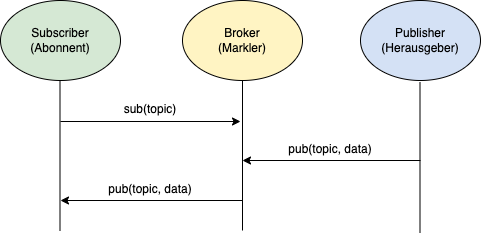
\includegraphics[width=12cm,height=12cm,keepaspectratio]{images/sub-model.drawio.png}
                \caption{Themenbasiertes Pub/Sub Kommunikationsmodell \cite{Hunkeler2008}}
                \label{pic:pub-sub-model}
            \end{figure}
            \\
            Dieses Prinzip ist ein essentieller Bestandteil des \acs{MQTT}-Protokolls. Im Folgenden wird ein Beispiel aufgezeigt, welches 
            die Kommunikation über das Publish/Subscribe Modell darstellt.
            
            \subsubsection*{Beispiel}
            \label{subsubsec:pubsub-example}
            IST NOCH AUSZUARBEITEN. BEISPIELBESCHREIBUNG FOLGT!!!! 
            %TBD 
            \begin{lstlisting}[language=Java, frame=lines, xleftmargin=\parindent, style=algoBericht, label={code:entity}, captionpos=b, caption={Test test}]
                subscribe -topic: test/test/
            \end{lstlisting}
            % Erläutern des Beispiels anhand des publishen und subscriben eines topics in bezug auf das checkin mit der authentifizierung und dem 
            % Command an Temi, welcher dann die Begrüßung und das Checkin durchführt. 


    \subsection{AMQP}
    \label{subsec:amqp}
        Das \ac{AMQP}-Protokoll ist ebenso ein leichtgewichtiges \acs{MtoM}-Protokoll, welches im Jahre 2003 von John O\'Hara JPMorgan Chase 
        in London, Großbritannien, entwickelt wurde \cite{Naik2017}. Der Fokus diesen Protokolls liegt auf der Unternehmens-Messaging Ebene 
        und legt hohen Wert auf die Zuverlässigkeit, Sicherheit, Bereitstellung und Interoperabilität der Kommunikation. \acs{AMQP} 
        unterstützt neben der Publish/Subscribe- auch die Request/Response Architektur. Es bietet eine breite Palette von 
        Funktionen im Zusammenhang mit Messaging, wie z. B. zuverlässiges Queuing, themenbasiertes Publish-and-Subscribe-Messaging, 
        flexibles Routing und Transaktionen \cite{Naik2017}. Das Kommunikationsmodell nach dem \acs{AMQP} Standard erfordert, dass der 
        Herausgeber (publisher) oder der Empfänger (subscriber) einen \textit{Austausch (exchange)} mit einem bestimmten Namen generiert 
        und diesen dann sendet \cite{Naik2017}. Die beiden Komponenten, Empfänger und Herausgeber, nutzen den Namen des Austausch, um eine 
        Verbindung aufzubauen. Der Empfänger erstellt darauf eine Warteschlange (queue) und hängt diese an den Austausch an. Nachrichten, die 
        über diese Verbindung ausgetauscht werden, müssen über einen gesonderten Prozess (binding) mit der Warteschlange abgeglichen werden 
        \cite{Naik2017}.
        \\ 
        Das binäre Protokoll \acs{AMQP} erfordert einen Header von acht Byte mit Nachrichtennutzlasten, die die Größe der Nachricht ist abhängig 
        von dem Broker, bzw. dem Server. Die Verbindungsorientierte Kommunikation von \acs{AMQP} basiert auf dem Standard-Transportprotokoll 
        \acs{TCP} und zur Sicherheit auf dem \acs{TLS}/\acs{SSL}-Protokoll. Ein Kernmerkmal des \acs{AMQP} Kommunikationsmodells ist die 
        Zuverlässigkeit \cite{Naik2017}. 
        \\
        \linebreak
        Neben den beiden aufgeführten Kommunikationsmodellen gibt es noch weitere, darunter das klassische \ac{HTTP} und das \ac{COAP}, die 
        allerdings nicht weiter ausgeführt werden. Der Fokus in dieser Arbeit liegt auf dem \acs{MQTT}-Protokoll. 
        
        %Vergleich in den Anhang packen??
        %\subsubsection*{Vergleich von MQTT und AMQP}
        %\label{subsubsec:mqtt-vs-amqp}
        %\begin{table}[hbt!]
        %    \begin{center}
        %        \begin{tabular}{| p{3.25cm} | p{6cm} | p{6cm} | }
        %            \hline
        %                \textbf{Kriterium} & \textbf{MQTT} & \textbf{AMWP}\\
        %            \hline
        %                Jahr & 1999 & 2003 \\ 
        %            \hline
        %                Architektur & Client/Broker, & Client/Broker Client/Server \\ 
        %            \hline
        %                Abstraktion & Publish/Subscribe & Publish/Subscribe Request/response \\ 
        %            \hline
        %                Header Größe & 2 Byte,  & 8 Byte \\ 
        %            \hline
        %                Nachrichtengröße & max. 265 MB & Abhängig von Broker/Server \\ 
        %            \hline 
        %                Semantik / Methoden & Connect, Disconnect, Publish, Subscribne, Unsubscribe, Close & Consume, Deliver, Publish, Get, Select, Ack, Delete, Nack, Recover, Reject, Open, Close \\
        %            \hline
        %                Zwischenspeicher (Cache) und Proxy & Teilweise & Ja \\
        %            \hline
        %                Standards & OASIS, Eclipse Foundation  & OASIS, ISO/IEC \\ 
        %            \hline
        %                Transport-Protokoll & TCP, & TCP, SCTP \\
        %            \hline
        %                Sicherheit & TLS/SSL & TLS/SSL \\ 
        %            \hline
        %                Standard-Port & 1883/8883 (TLS/SSL) & 5671 (TLS/SSL), 5672 \\
        %            \hline
        %                Format & binär  & Binär \\ 
        %            \hline
        %                Lizenzmodell & Open Source & Open Source \\
        %            \hline
        %                Support & IBM, Facebook, Eurotech, Cisco, Red Hat Amazon (AWS) etc. & Microsoft, JP Morgan, Bank of America, Barclays, Goldman Sachs Credit Suisse \\ 
        %            \hline
        %        \end{tabular}
        %    \end{center}
        %    \caption{Vergleich von MQTT und AMQP \cite{Naik2017}}
        %    \label{tab:mqtt-vs-amqp}
        %\end{table}
        
        
        %Dadurch wird die Konfiguration und Einsetzbarkeit der Technologie komplexer im Gegenzug zu MQTT


        % Vergleich zu MQTT

    
    % Überlegen, bzw. abwarten, ob das benötigt wird.... 
    %\subsection{Raspberry Pi}
    %\label{subsec:raspberrypi} 

%\section{Roboter}
\subsection{Serviceroboter}
\subsection{Temi - Roboter}
\section{Home Assistant}
\label{sec:homeassistant}
    Eines der populärsten \acl{SH} Plattformen ist das sogenannte Home Assistant System. Die Open-Source-Software ist ein zentrales 
    Steuerungssystem von Heimautomationen und der Verwaltung von intelligenten Geräten mit dem Fokus der lokalen Steuerung und gesicherter 
    Privatsphäre. Der Zugriff kann über die Smartphone-App, jeweils verfügbar für iOS und Android, oder auch über die webbasierte 
    Benutzeroberfläche (Web-App) erfolgen. In dem lokalen System können auch Geräte die Steuerung per Sprachbefehlen ermöglichen. Kompatible 
    Plattformen sind unter anderem Google Assistant, Amazon Alexa und Apple HomeKit. Dies sind weitaus nur eine Selektion von bekannten 
    Herstellern. Home Assistant bietet eine weitaus vielfältigere Verknüpfung von Geräten, Services und Plattformen. Die zentrale Steuerung 
    unterstützt durch modulare Integrationskomponenten die einzelnen Geräte, Anwendungen und Services. Für die drahtlose Kommunikation 
    werden native Integrationskomponenten verwendet, darunter Bluetooth, ZigBee und Z-Wave. Diese werden verwendet, um lokale \ac{PAN} mit 
    Geräten mit geringem Stromverbrauch aufzubauen. Die Steuerung kann auch mit Proprietären Ökosystemen stattfinden, sofern diese eine offene 
    \acs{API} oder Anbindungen über \acs{MQTT} anbieten.\footnote{Grundlegende Ableitung der Definition von Home Assistant siehe \url{https://en.wikipedia.org/wiki/Home_Assistant} Abgerufen am 16.04.2022}
    \\
    Die Platform ist in Python geschrieben und wird aktiv instand gehalten und durch eine große Community unterstützt. Die Software ist allgemein unter 
    der Apache 2.0, veröffentlicht. Der folgende Abschnitt befasst sich in Kürze mit der Historie des Systems. 
    
    \subsection*{Historie}
    \label{sec:historyHOAS}
        Anfang des vierten Quartals im Jahr 2013 startete das Python-Projekt von Paulus Schoutsen und im November 2013 erstmals auf GitHub 
        veröffentlicht.\footnote{Anfänge von Home Assistant. \url{https://www.linux.com/topic/embedded-iot/home-assistant-python-approach-home-automation/} Abgerufen am 18.04.2022}
        \\
        \linebreak
        Vier Jahre nach den ersten Entwicklungen der \acl{SH} Plattform wurde im Juli 2017 ein verwaltetes Betriebssystem mit dem Namen 
        \textit{Hass.io} entwickelt.\footnote{Verkündungen von Home Assistant. \url{https://www.home-assistant.io/blog/categories/announcements/} Abgerufen am 18.04.2022} 
        Dadurch gelang der Durchbruch der vereinfachten Verwendung von der Home Assistant Plattform auf kleineren Computern, sogenannten 
        Einplatinencomputern, wie beispielsweise einem der Raspberry Pi Serie. In Zusammenhang mit dem Betriebssystem kam ein 
        \textit{Supervisor}-Verwaltungssystem hinzu, das den Benutzern die Verwaltung, Sicherung und Aktualisierung der lokalen Installation 
        ermöglicht. Ein weiteres Feature des Supervisors ist die Möglichkeit der Plattform über Add Ons weitere Funktionalitäten zu Verfügung zu 
        stellen.\footnote{Einstieg in das Hass.io Betriebssystem. \url{https://www.home-assistant.io/blog/2017/07/25/introducing-hassio/} Abgerufen am 18.04.2022}
        \\
        \linebreak
        Die Software wird stetig weiterentwickelt und verbessert. Mittlerweile gehört sie zu den am meist genutzten Open-Source-Plattformen 
        im Bereich \acl{SH}.

\subsection{Konzept und Architektur}
\label{sec:conceptArchitectureHAOS}
    Home Assistant bietet eine Plattform für die zentrale Haussteuerung und die damit einhergehende Steuerung von Heimautomationen. Die 
    Software ist nicht nur eine einfache Steuerungs- und Konfigurations-Software, sondern ein eingebettetes Betriebssystem, das 
    verbraucher- und nutzerorientiert das Verwenden und Konfigurieren von Haussteuerungen erleichtert. \footnote{Konzept und Architektur von Home Assistant. \url{https://developers.home-assistant.io/docs/architecture_index} Abgerufen am 19.04.2022}
    \\
    \linebreak
    Damit der offene Ansatz von Home Assistant Anbietern gegenüber nicht eingeschränkt ist, bietet die Software Möglichkeiten, um viele 
    Geräte zu vereinheitlichen. Somit begegnet Home Assistant der Heterogenität des offenen Marktes, in sofern, dass diese Geräte auf  
    gemeinsame Konzepte gebracht werden. Diese sind in vier Konzepte\footnote{Erläuterung der Konzepte von Home Assistant. \url{https://apiumhub.com/tech-blog-barcelona/domotics-with-home-assistant-concepts/} Abgerufen am 21.04.2022} 
    aufgeteilt, mit der die Vereinheitlichung vorangetrieben werden kann: 
    \begin{itemize}
        \item Integration (Integration): Integrationen repräsentieren die Geräte und Dienste innerhalb der Home Assistant Anwendung. 
              Ebenso können mittels den Integrationen auch Daten von Datenpunkten abgerufen werden.
        \item Gerät (Device): Nach der Konfiguration der Integration werden die Geräte in Home Assistant angelegt. 
              Diese werden dann als erkannte Geräte der Integration dargestellt, z.B. als Temperatur-, Licht- oder Feuchtigkeitssensor.
        \item Entität (Entity): Die Datenpunkte sind die Geräte, die sogenannten Entitäten, die durch die Integrationen standardisiert werden. 
              Dies sin Objekte, die Funktionalitäten oder Daten des Geräts darstellen, z.B. die Temperatur, Helligkeit oder die Feuchtigkeit.
        \item Automatisierung (Automation): Automatisierungen sind Prozesse, die bei einem bestimmten ausgelösten Event ausgeführt werden 
              sollen. Dieses Auslöser (trigger) können Zeitpunkte, Ereignisse oder manuell gesteuerte Aktionen des Nutzers sein, z.B. das 
              Ausschalten des Bürolichts, wenn durch einen Bewegungssensor fünf Minuten keine Bewegung festgestellt wurde oder wenn der 
              Helligkeitswert, der über den Sensor festgestellt wurde einen bestimmten Wert erreicht hat, soll das Licht ebenso 
              ausgeschaltet werden.
    \end{itemize}
    Die Architektur der Home Assistant Anwendung ist grundlegend als eingebettetes System eines Betriebssystem aufgestellt, welches in 
    drei Schichten aufgeteilt ist. In unterster Ebene befindet sich das Betriebssystem, welches als minimales Linux System aufgestellt 
    ist, um die darauf liegenden Schichten, den Aufseher (supervisor) und den Kern (core), zu betreiben. Mit dem Supervisor wird das 
    Betriebssystem verwaltet und konfiguriert. Der eigentliche Kern interagiert mit dem Supervisor, den Geräten und den Services. 
    %Erläuterung supvervisor und core Architektur
    \\
    \linebreak
    Der Supervisor ist die Schicht über dem Betriebssystem. Die Kommunikation der beiden Komponenten findet die über einen D-Bus statt. Diese Zwischenschicht ermöglicht dem 
    Benutzer die Verwaltung der Home Assistant Installation. 
    \\
    Die Aufgaben des Supervisors sind wie folgt 
    definiert\footnote{Architektur des Home Assistant Supervisors. \url{https://developers.home-assistant.io/docs/supervisor} Abgerufen am 22.04.2022}: 
    \begin{itemize}
        \item Dieser führt den Home Assistant Kern (Core) aus.
        \item Dieser führt die Updates des Home Assistant Core aus.
        \item Dieser führt einen \textit{Rollback} bei Fehlgeschlagenem Update durch.
        \item Dieser führt Sicherungen und Wiederherstellungen durch.
        \item Dieser verwaltet die Add Ons der Core Instanz
    \end{itemize}
    \begin{figure}[hbt!]
        \centering
        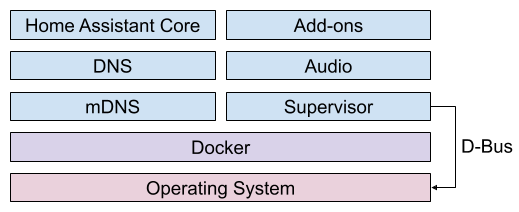
\includegraphics[width=10cm,height=10cm,keepaspectratio]{images/ha_architecture_2020.png}
        \caption{Architektur des Home Assistant Supervisors}
        \label{fig:architectureHAOS}
    \end{figure}
    Die auf dem Supervisor aufbauende Architektur ist die Architektur der Anwendung, der sogenannte Core. Dieser besteht aus vier 
    Komponenten, welche den Hauptteil abbilden: Event Bus, State Machine, Service Registry und Timer\footnote{Entwickler Dokumentation der Home Assistant Plattform. \url{https://developers.home-assistant.io/docs/} Abgerufen am 24.04.2022}. 
    \\
    Mit dem Event Bus wird das Abhören und Auslösen von Events und Ereignisse erleichtert. Die Komponente stellt eine zentrale Eigenschaft 
    der Home Assistant Anwendung dar. Die Zustandsmaschine (State Machine) ist eine weitere Komponente, mit der die Zustände von Dingen, darunter 
    intelligente Geräte, Sensoren uvm., überwacht und Zustandsänderungsereignisse an den Event Bus ausgelöst werden. Dies erfolgt nach der 
    Änderung des Zustandes eines Objektes. Mit der Dienstregistrierung (Service Registry) wird der Event Bus auf eingehende Aufrufe von 
    Diensten abgehört. Über die Service Registry kann der Benutzer Dienste hinzufügen und verwalten. Mittels den Entwicklertools, die über das 
    \ac{UI} aufgerufen werden können, kann der Benutzer die Dienste und Automatisierungen aufrufen und konfigurieren. Das letzte 
    Element, der Timer, ist ebenso eine Komponente der Architektur, die zeitveränderte Ereignisse gemäß einer gegebenen Frequenz 
    an den Event Bus sendet. Somit können zeitbasierte Automatisierungen vereinfacht und ausgelöst werden. Als Datenbank wird eine 
    nicht Cloud-basierte SQLite\footnote{Structured Query Language, eine Datenbanksprache zur Definition, Abfrage und Bearbeitung von Datenstrukturen in relationalen Datenbanken} 
    Datenbank verwendet. Diese ist nur auf dem Gerät enthalten und wird nicht über das Internet übertragen. 
    Im lokalen Netzwerk hat der Nutzer die Möglichkeit, um auf die Datenbank zuzugreifen und eine Historie von Aktionen einzusehen. 
    Eine Verlaufskomponente, die ebenso im Core enthalten ist, speichert die Ereignisse innerhalb der Plattform. Somit können Nutzer auf 
    alle gespeicherten Informationen zu Hause zugreifen und diese einsehen \cite{HAOSarchitecture2018}.
    \\
    \linebreak
    \begin{figure}[hbt!]
        \centering
        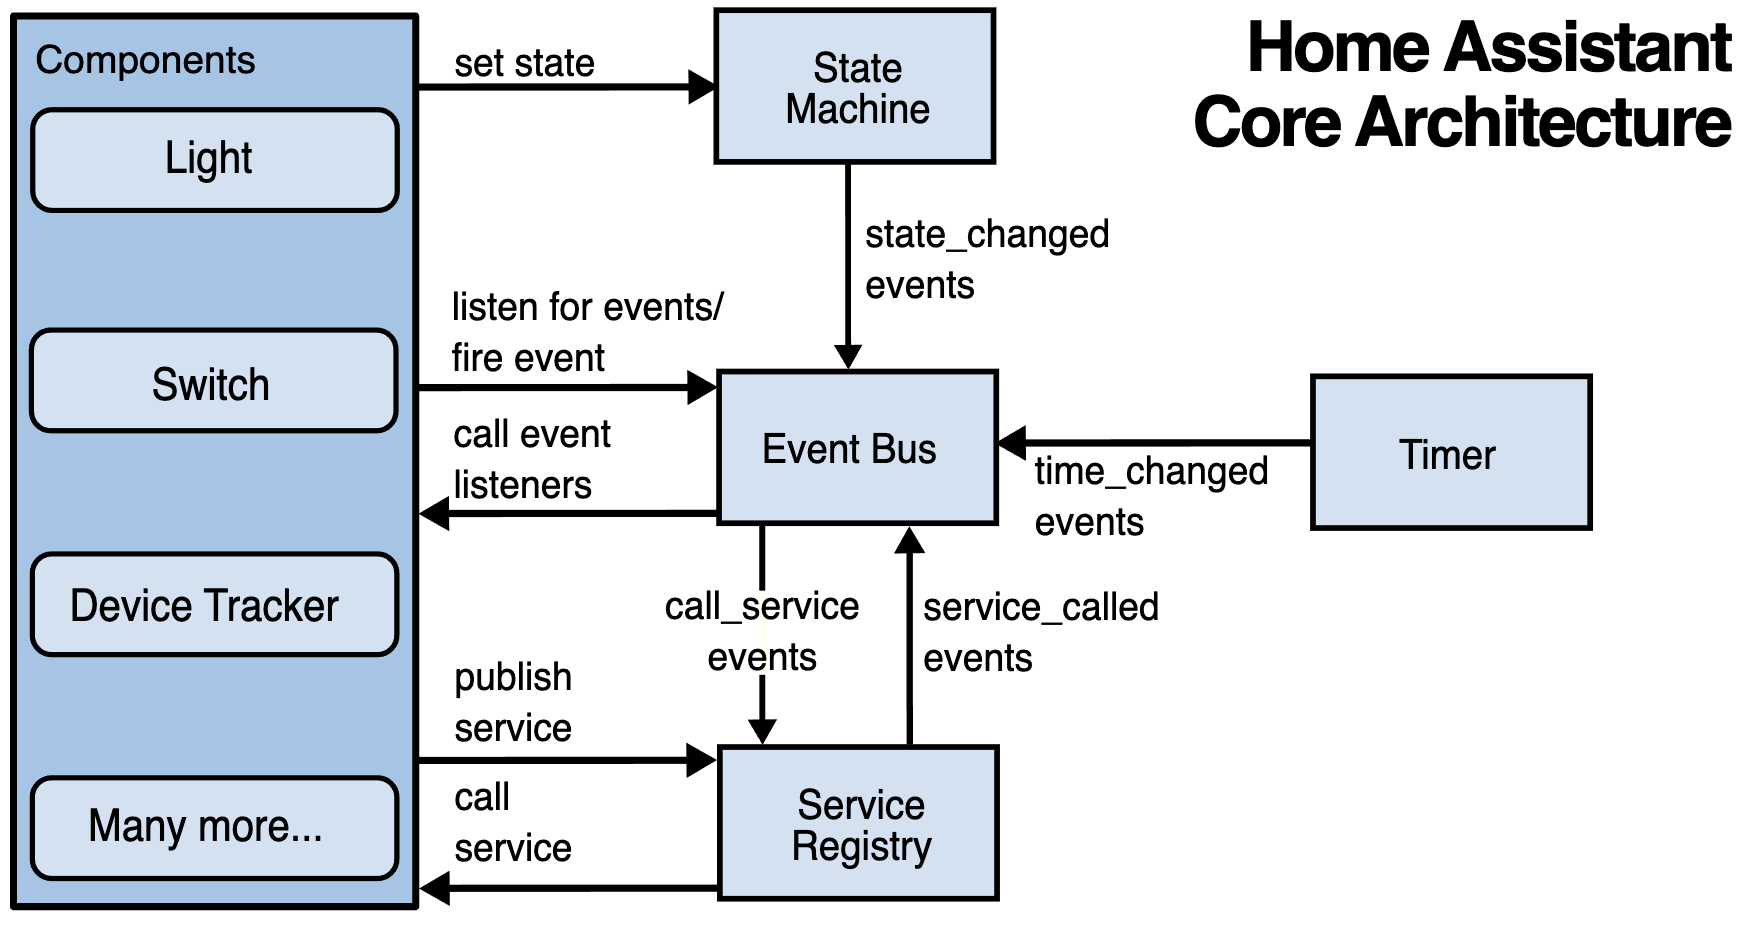
\includegraphics[width=15cm,height=15cm,keepaspectratio]{images/HAOS_Core_Architecture.png}
        \caption{Architektur des Home Assistant Cores \cite{HAOSarchitecture2018}}
        \label{fig:architectureHAOSCore}
    \end{figure}
\subsection{Ziele und Schwerpunkte}
    Jede Softwarelösung verfolgt bestimmte Ziele und Schwerpunkte, damit die Zielerreichung (\ac{DOD}) messbar ist. Die mit 
    der Home Assistant Plattform verfolgten Ziele sind Privatsphäre und Sicherheit, die Wahlmöglichkeiten von Geräten und die Haltbarkeit 
    der Plattform\footnote{Schwerpunkte der Home Assistant Plattform. \url{https://www.home-assistant.io/blog/2021/12/23/the-open-home/} Abgerufen am 24.04.2022}. 
    \\
    \linebreak
    Das Thema der Privatsphäre wird bei Home Assistant dadurch forciert, dass die Geräte nur optional über das Internet erreichbar sind, bzw. 
    nur über das lokale Netzwerk. So kann die Kategorisierung des Verhaltens durch Algorithmen vermieden werden. 
    \\
    Die großflächige Auswahlmöglichkeit von Geräten und Verknüpfungen ist ein weiteres großes Ziel von Home Assistant, da es möglich ist  
    herstellerunabhängig Geräte zu verwenden und zu integrieren. Dadurch können über eine Zentrale mehrere Geräte von diversen Herstellern 
    kombiniert werden.
    \\
    Haltbarkeit wird an der Stelle adressiert, an der die Plattform uneingeschränkt verfügbar ist und Geräte zur Anbindung verwendbar sind. 
    Damit ist auch zu erwarten, dass Geräte, die eingebunden werden können, so konzipiert und gebaut sind, damit sie eine lange Lebensdauer 
    besitzen.
    \\
    \linebreak
    Schwerpunkte, bzw. Lösungen zur Problembehebung sind die Kontrollierbarkeit über eine einzige zentrale Stelle und die Konfiguration von 
    Automationen, die Prozesse selbstständig auslöst. Durch die Möglichkeit der Automatisierung und Steuerung von Komponenten im Eigenheim, 
    bzw. im Büro kann die Lebensqualität erhöht als auch die Energy- und Stromkosten gesenkt werden. Die Kompatibilität der Plattform 
    ermöglicht die Verwendung von mehreren Geräten und Herstellern über eine zentrale Stelle, der Home Assistant Software. Dies ermöglicht 
    dem Nutzer die uneingeschränkte Verwendung von Geräten und die Unabhängigkeit zu Herstellern, die ggf. den Preis der Geräte über dem 
    Marktdurchschnitt verkaufen. Ein weiterer Schwerpunkt ist die Sichtbarkeit der Daten, die potentiell gesendet werden, um den Datenschutz 
    und die Privatsphäre auf dem höchsten Standard zu halten. Ein Auswirkung dafür ist die zugrundeliegende lokale Datenhaltung über die 
    Datenbank, die direkt auf dem Gerät der Plattform läuft.

    %https://apiumhub.com/tech-blog-barcelona/domotics-with-home-assistant-concepts/
    %Home Assistant is created to address these issues:
    %– Could we have a single home automation/control centre, compatible with almost all electronic devices?
    %– Could we make the sending of data to an external server visible? Could we even eliminate it completely?

\subsection{Stärken und Schwächen}
    Die Stärken und Schwächen der Plattform belaufen sich auf die folgenden Aspekte:
    \begin{table}[hbt!]
        \begin{center}
            \begin{tabular}{| p{7.875cm} | p{7.785cm} | }
                \hline
                    \textbf{Stärken} & \textbf{Schwächen} \\
                \hline
                    Open-Source Software & Schwerer Einstieg für neue Nutzer im Hinblick auf die Konfiguration der Automationen \\ 
                \hline
                    Privatsphäre \& Datenschutz & Automationen im YAML-Datenformat und benutzerdefinierte Komponenten können für neue Benutzer schwierig sein \\ 
                \hline
                    Große Community & Langwierige Installationen von Integrationen \\ 
                \hline
                    Automationen sind sehr mächtig & Die Erweiterung, Einrichtung und Konfiguration erfordert die Bearbeitung von YAML-Dateien und einen Neustart bei jeder Änderung \\ 
                \hline
                    Stetige Aktualisierung, Weiterentwicklung und Fehlerbehebung & Automationen können kompliziert aufgebaut sein \\ %  (User Interface zur Erstellung von Automationen wäre für nicht IT-Affine Anwender angebracht.)
                \hline 
                    Unterstützung vieler Geräte (Herstellerunabhängigkeit) und großflächige Kompatibilität & Nutzung von ZigBee und Z-Wave erfordert jeweils eigene Konfigurationen, welche die All-in-One Lösung erschwert. \\
                \hline
                    Individuelle Modifikation der UI &  \\ 
                \hline
                    Kann auf beliebiger Hardware ausgeführt werden &  \\
                \hline
            \end{tabular}
        \end{center}
        \caption{Stärken und Schwächen der Home Assistant Plattform}
        \label{tab:prosConsHAOS}
    \end{table}
    \\
    %Die Auflistung der Punkte geht aus Beiträgen der Community und dokumentierten Erfahrungen der Anwendung. 
    Die Konfiguration von Automationen, Funktionen und Integrationen über YAML-Dateien kann auf der einen Seite als Stärke gewertet werden, 
    da die Syntax flexibel einsetzbar ist und Freiheiten bei der Implementierung bietet und auf der anderen Seite als Schwäche, da die 
    Konfigurationen schnell unübersichtlich werden und anfangs schwer zu verstehen sind. Der Aufwand steigt je nach zu implementierende 
    Funktion und deren Abhängigkeiten zu Geräten und gegebenenfalls zu anderen Prozessen und Automationen. 

\section{openHAB}
\label{sec:openhab}
    Neben der so eben erläuterten Home Assistant Plattform zählt ebenso die openHAB Plattform als bekannt und 
    in der Anwendung populär. Der \ac{OPENHAB} ist eine Plattform, bei der es sich um eine 
    Softwarelösung handelt, die auf Basis der Programmiersprache Java aufgebaut ist. Die Software steht unter 
    der Eclipse Public License und fällt daher unter die Rubrik der Open-Source Software. Durch die Verwendung 
    von Java ist die Anwendung betriebssystemunabhängig und kann auf beliebigen Betriebssystemen laufen. 
    Ähnlich zu der vorgestellten Home Assistant Software, bietet openHAB ebenso User Interfaces die durch 
    den Webbrowser, Android- und iOS-Geräte unterstützt werden. 
    \\
    \linebreak
    In Kombination mit Java wird bei openHAB das \ac{OSGI}-Framework für die Modularität der Software verwendet. Mit Apache 
    Karaf wird ein Container bereitgestellt, der mit Eclipse Equinox als \acs{OSGI} Laufzeitumgebung agiert. Als 
    \acs{HTTP}-Server ist Jetty in Gebrauch. Die einzelnen Frameworks werden nicht im Detail erläutert, lediglich die für das 
    Verständnis des Konzeptes notwendigen.
    \\
    \linebreak
    Mit openHAB wird eine hochmodulare Software zur Verfügung gestellt, die durch sogenannte \textit{Add-ons} erweitert 
    werden kann. Durch diese wird der Plattform eine breite Palette an Funktionen geboten. Physische Geräte können in 
    großer Anzahl mit der Plattform interagieren und verknüpft werden.\footnote{Einleitung zu openHAB. \url{https://www.openhab.org/docs/} Abgerufen am 25.04.2022}

    \subsection*{Historie}
    \label{sec:historyoHAB}
    %TBD...

\subsection{Konzept und Architektur}
%\subsection{Architektur}
    Die Steuerungsplattform openHAB bietet vergleichbar zu Home Assistant die Möglichkeit der multifunktionalen Verknüpfung von 
    Geräten und Protokollen. An dieser Stelle werden ebenso mehrere Konzepte verwendet, die die Vereinheitlichung der Plattform 
    verstärkt. Die Konzepte der openHab Software sind in drei größere Rubriken aufgeteilt, die sich wie folgt zusammensetzen:
    \\
    \linebreak
    Die erste Rubrik sind die Dinge (Things), diese sind die Entitäten, die als physische Komponente zu einem System hinzugefügt 
    und viele Funktionalitäten als eines bereitstellen kann. Hierbei ist zu berücksichtigen, dass die sogenannten Dinge nicht 
    immer Geräte sein müssen, diese können auch andere überschaubare Informationsquellen, andere Webdienste und Funktionalitäten 
    darstellen. Aus Sicht des Benutzers sind sie für den Einrichtungs- und Konfigurationsprozess relevant, für den Betrieb 
    jedoch potentiell zu vernachlässigen. Dinge können Konfigurationseigenschaften haben, die optional oder obligatorisch sein 
    können. Solche Eigenschaften können grundlegende Informationen wie eine IP-Adresse, ein Zugriffstoken für einen Webdienst 
    oder eine gerätespezifische Konfiguration sein, die sein Verhalten ändert \cite{openHAB-article}. Mit dem Konzept der Dinge 
    kommen zwei Unterkategorien einher:
    \begin{itemize}
        \item Kanäle (Channels): Jedes Gerät, bzw. Ding stellt Kanäle bereit, mit denen die jeweiligen Funktionen abgebildet werden. 
        An der Stelle an der das physische Gerät angebunden ist, ist der Kanal eine konkrete Funktion dieser Entität. Beispielsweise 
        kann eine Glühbirne einen Kanal für die Farbtemperatur und einen für den Farbwert besitzen. Diese stellen beide die 
        Funktionalität der einen physischen Glühbirne für das System bereit. Grundlegend sind Kanäle mit Elementen verknüpft, mit denen 
        die virtuelle und physische Ebene verbunden wird. Ab dem Zeitpunkt, sobald eine Verbindung hergestellt wird, reagiert ein Ding 
        auf Ereignisse, die für ein Element transferiert werden. Bedingung dafür ist die Verknüpfung zu einem Kanal. Auf der anderen 
        Seite werden aktiv Ereignisse für Objekte gesendet, die mit Kanälen des Dings verknüpft sind \cite{openHAB-article}.
        \item Brücken (Bridges): Die Brücke ist eine besondere Art von Ding. Diese müssen dem System hinzugefügt werden, damit der 
        Zugriff auf andere Dinge ermöglicht wird, bzw. erhalten bleibt. Ein IP-Gateway für Hausautomationssysteme, welches nicht 
        IP-basiert funktioniert, ist eine typisches Beispiel für so eine Brücke.
    \end{itemize}
    An zweiter Stelle stehen die Artikel (Items). Diese Elemente stellen Funktionen dar, die direkt von der Anwendung verwendet 
    werden. Darunter zählen hauptsächlich die Automatisierungslogik oder auch Benutzeroberflächen. Durch Ereignisse werden die 
    Elemente verwendet, da diese einen Zustand besitzen. 
    \\
    Elemente können auch in eine Gruppe zusammengefasst werden. Ein Gruppenelement kann auch Mitglied einer weiteren Gruppe sein. 
    Diese zyklischen Mitgliedschaften sind war nicht verboten, davon wird jedoch abgeraten. Über Benutzeroberflächen können 
    einzelne Gruppenelemente als alleinstehender Eintrag angezeigt werden und eine Navigation zu den jeweiligen Mitgliedern 
    bereitstellen. 
    \\
    \linebreak
    Die dritte große Rubrik sind die Bindungen und Links (Bindings and Links). Diese können als Softwareadapter betrachtet werden, 
    die Dinge für ihr Hausautomationssystem zur Verfügung stellen \cite{openHAB-article}. Aufgabe der Komponente ist die Verknüpfung 
    von Elementen mit physischen Geräten. Um dies zu ermöglichen werden die spezifischen Kommunikationsanforderungen eines Geräts 
    abstrahiert. Dadurch ist eine allgemeinere Behandlung der Komponente durch das Framework möglich. Links stellen das Bindeglied 
    zwischen Dingen und Gegenständen dar. Es ist die Verknüpfung von genau einem Element und einem Kanal. Elemente und 
    Kanäle haben keine eins zu eins Beziehung zueinander. Eine Verknüpfung mit mehreren Komponenten ist auch hier möglich. 
    \\
    \linebreak
    Die Architektur der openHAB Anwendung %TBD 
    \begin{figure}[hbt!]
        \centering
        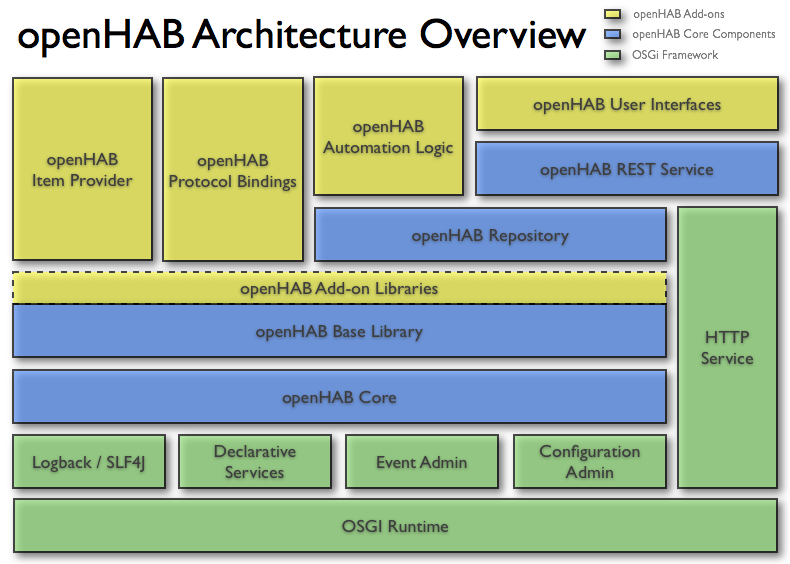
\includegraphics[width=15cm,height=15cm,keepaspectratio]{images/openhab-architecture.png}
        \caption{Architektur der openHAB Plattform \cite{openHAB-architecture2018}}
        \label{fig:architectureopenHAB}
    \end{figure}




\subsection{Ziele und Schwerpunkte}
\subsection{Stärken und Schwächen}

\section{Vergleich von Home Assistant und openHAB}
\label{sec:comparison-HAOS-openHAB}
    %Allgemein gültiger Vergleich (Aufbau, Architektur, Schwerpunkte (Fokus), Umsetzungen, Konnektivität, etc.)
    % https://everythingsmarthome.co.uk/home-assistant-vs-openhab-which-one-is-better/
    % https://smarthome.msuttner.de/openhab-2/vergleich-openhab-vs-home-assistant/ 
    % https://www.electronicshub.org/openhab-vs-home-assistant/ 
    % https://smarthome.university/your-smart-home-platform-home-assistant-vs-openhab/ 


%\section{Requirements Engineering}
\label{sec:requirementsengineering}
    In der heutigen Softwareentwicklung ist zu Anfang jedes Projekts die Frage offen, welche Anforderungen soll das 
    Produkt erfüllen, sodass daraus eine gute, stabil und effiziente Software entsteht und der Umfang und das Ziel 
    klar gestaltet sind. Mit dem \acl{RE} wird der Gedanke verfolgt, die Bedürfnisse des Kunden, bzw. des Stakeholders 
    zu erfüllen und eine erfolgreiche, den Kunden zufriedenstellende Entwicklung des Systems zu erzielen. Ein Stakeholder 
    ist eine Person oder Organisation mit Einfluss auf die Anforderungen des Systems oder die Auswirkungen auf das System 
    hat \cite{pohl2021basiswissen}.
    Diese Anforderungen werden durch das \acl{RE} ermittelt und dokumentiert. 
    \\
    \linebreak
    Unter dem Begriff \ac{RE} ist folgendes zu verstehen: 
    \begin{quote}
        Das Requirements Engineering ist ein systematischer und disziplinierter Ansatz zur Spezifikation und zum 
        Management von Anforderungen mit dem Ziel, die Wünsche und Bedürfnisse der Stakeholder zu verstehen und 
        die Gefahr zu minimieren, ein System auszuliefern, das diese Wünsche und Bedürfnisse nicht erfüllt. \cite{pohl2021basiswissen}
    \end{quote}
    Oft wird darunter auch ein kooperativer und inkrementeller Prozess verstanden, dessen Ziele die Gewährleistung 
    folgender Punkte darstellt:
    \begin{itemize}
        \item Alle Anforderungen sind bekannt und werden auch in dem erforderlichen Detaillierungsgrad verstanden.
        \item Alle involvierten Stakeholder haben eine ausreichende Übereinstimmung über die bekannten Anforderungen erzielt.
        \item Alle Anforderungen sind zu den Dokumentationsvorschriften konform, bzw. zu den Spezifikationsvorschriften konform spezifiziert.
    \end{itemize}
    Damit ist von System-Design, Architekturen oder die nachfolgenden Tests zu differenzieren. 
    \\
    Dieser Prozessschritt deckt die Formalitäten ab, um allen beteiligten eine grundlegende Übersicht zu geben, welche 
    Ziele verfolgt werden, bzw. welche Anforderungen erfüllt werden sollen. Auch ist das \acl{RE} ein wesentlicher 
    Bestandteil des Entwicklungsprozesses nach Scrum. Unter dem Begriff Scrum ist ein Vorgehensmodell zu verstehen, 
    welches zum Projekt- und Produktmanagement in agilen Softwareentwicklungen eingesetzt wird. 
    \\
    \linebreak
    Innerhalb der Anforderungen, die im \acl{RE} ermittelt werden, wird zwischen drei Arten von Anforderungen unterschieden: 
    \begin{itemize}
        \item Funktionale Anforderungen: Diese legen die Funktionalität fest, die durch die Entwicklung des Systems 
            erreicht werden soll. Typischerweise werden diese in Funktions-, Verhaltens- und Strukturanforderungen unterteilt.
        \item Qualitätsanforderungen: Diese legen die Qualitäten des Systems fest und beeinflussen die Gestaltung der 
            Systemarchitektur in größerem Maß als die funktionalen Anforderungen.
        \item Randbedingungen (Constraints): Diese legen die Randbedingungen des Systems fest.
    \end{itemize}
\chapter{Stand der Technik}
Stand der Technik
\section{Theorien}
\section{Methoden}
\section{Techniken}

\chapter{Anforderungsanalyse}
\label{chap:anforderungsanalyse}
    Dieses Kapitel befasst sich im Allgemeinen mit der Anforderungsanalyse und -erhebung. Hierbei wird eine
    Marktanalyse repräsentiert, um das Potential rundum \acl{SH} aufzuzeigen und ein Gefühl 
    dafür zu vermitteln, welche Anforderungen dabei entstehen können, bzw. bereits bestehen. Die Analyse ist 
    mit repräsentativen Statistiken, Studien und Umfragen belegt. Hauptsächlich wird im Rahmen der Anforderungserhebung 
    auf die Methodiken und Techniken eingegangen, die verwendet werden, um 
    Anforderungen zu identifizieren. Diese dienen als Grundlage für die Konzeption der Steuerzentrale. Bestandteile der 
    Anforderungserhebung sind unter anderem zentrale Prozesse des \acl{RE}, ein \textit{user-centered Design}, im Deutschen 
    nutzerzentriertes Design, eine \textit{Target Group Analysis}, im Deutschen Zielgruppenanalyse, und die Durchführung von 
    Experten Interviews. Diese Interviews sind nicht repräsentativ und dienen lediglich der weiträumigeren Informationsgewinnung. 
    \\
    Vorab wird sichergestellt, dass im Rahmen des benutzerzentrierten Designs der Softwareentwickler als Nutzer und Anwender im 
    Vordergrund steht, da dieser die Plattform betreibt, bzw. für die Erweiterung der Software als auch für die 
    Anpassungen auf die eigenen Anwendungsfälle zuständig ist.
    \\
    \linebreak
    Damit ein Eindruck entsteht, welches Marktpotential \acl{SH} Anwendungen haben und welche Anforderungen somit 
    verbunden sind, wird basierend auf gegebenen Studien, Statistiken und Umfragen eine Marktanalyse durchgeführt.

\section{Marktanalyse}
\label{sec:marktanalyse}
    Der Markt rundum \acl{SH} nimmt immer weiter zu. Sei es die Entwicklung von neuen intelligenten Geräten, die 
    Massentauglichkeit von Geräten %, die nicht lange am Markt bestehen 
    oder die stetig wachsende Abdeckung von Anwendungsfällen und Übernahme von Aufgaben und Prozessen. Durch die Vielzahl an 
    Produktanbietern und diversen Kommunikationsmöglichkeiten, ist es schwierig eine Lösung für alle Alternativen und 
    Produktausprägungen anzubieten. Hersteller versuchen mit der angebotenen Produktpalette ihr eigenes Ökosystem im Bereich 
    \acl{SH} zu erstellen, um die Nutzer abhängig zu machen. Der repräsentativen Studie von Deloitte zufolge ist jedoch eine 
    Insellösung bei den Nutzern in Deutschland nicht gefragt \cite{deloitte2018}. Befragt wurden 2000 Konsumenten zwischen 
    19 und 75 Jahren. Einem geringen Anteil von 22 Prozent der 
    Befragten ist die Erweiterbarkeit des Systems mit Produkten anderer Hersteller weniger, bzw. nicht wichtig. Im Gegensatz dazu 
    empfinden 43 Prozent der Befragten die Erweiterbarkeit als wichtig und 28 Prozent als sehr wichtig \cite{deloitte2018}. 
    Demnach müssen die Hersteller eine flexiblere Einsetzbarkeit gewährleisten, damit solche Systeme den Marktdurchbruch 
    erlangen. Dadurch wird die Entwicklung von Plattformen komplexer und umfangreicher. Beispielsweise sind die am weit 
    verbreitetsten Open Source Plattformen, openHAB und Home Assistant, sehr komplex und bilden ein großes Ökosystem ab, da 
    stetig der Zuwachs an integrierbaren Geräten zunimmt und damit der Funktionsumfang steigt.  

    \subsection{Allgemeine Marktsituation und Marktprognose}
    %Anbieter, Plattformen, Geräte
        Derzeit gibt es viele Anbieter für intelligente Produkte. Diese bieten zum einen einzelne Geräte an, die in 
        beliebige Plattformen integriert werden können und zum anderen ein eigenes Ökosystem, sofern der Anwender 
        mehrere Produkte des Anbieters nutzen möchte. Dennoch ist in den meisten Fällen die Konfiguration der Geräte nur auf 
        den hauseigenen Plattformen möglich. Somit kann der Nutzer nicht alle Komponenten ausschließlich über eine Plattform 
        konfigurieren und steuern. 
        \\
        \linebreak
        Eine repräsentative Umfrage der \ac{SGCS} mit 1384 Teilnehmern, welche im April 2022 veröffentlicht wurde, zeigt, welche 
        Anbieter in Deutschland am meist verbreitetsten sind, bzw. welche die Nutzer am häufigsten kaufen. An oberster Stelle 
        steht Philips und Samsung mit jeweils 25 Prozent und an dritter Stelle Bosch mit 23 Prozent. Weitere Anbieter können dem 
        Diagramm im Anhang (siehe \ref{appendix:brandings}) entnommen werden. Dabei sind jedoch weitaus nicht alle Hersteller und 
        Anbieter aufgelistet. Detaillierter wird an dieser Stelle jedoch nicht eingegangen. 
        \\
        \linebreak
        Der aktuelle Markt für intelligente Produkte ist in sechs primäre Segmente aufgeteilt, die jeweils andere Anwendungsfälle 
        abdecken \cite{statista2021}:
        \begin{itemize}
            \item Kontrolle und Konnektivität: Gateways die alle Geräte jeglicher Segmente kontrollieren, intelligente Lautsprecher 
            mit dem Fokus zur Kontrolle und der digitalen Unterstützung und bspw. intelligente Steckdosen
            \item Intelligente Geräte (Smart Appliances): Kühlschrank, Waschmaschine und Geschirrspüler, Kaffeemaschine, Mikrowelle 
            und Staubsaugerroboter
            \item Sicherheit: Bewegungs-, Wasser- und Rauchmelder, Kameras und Türschlösser
            \item Heimunterhaltung (Home Entertainment): Fernseher, Entertainment-Systeme 
            \item Komfort und Licht: Intelligente LEDs, Fenster- und Tür-Sensoren etc.
            \item Energiemanagement: Thermostate und Regler, Luftqualitätsmesser etc. 
        \end{itemize}
        \pagebreak
        Die aufgelisteten Segmente werden von vielen Herstellern bedient. Darunter sind der folgenden Abbildung die 
        repräsentativen Schlüsselanbieter zu entnehmen:
        \begin{figure}[hbt!]
            \centering
            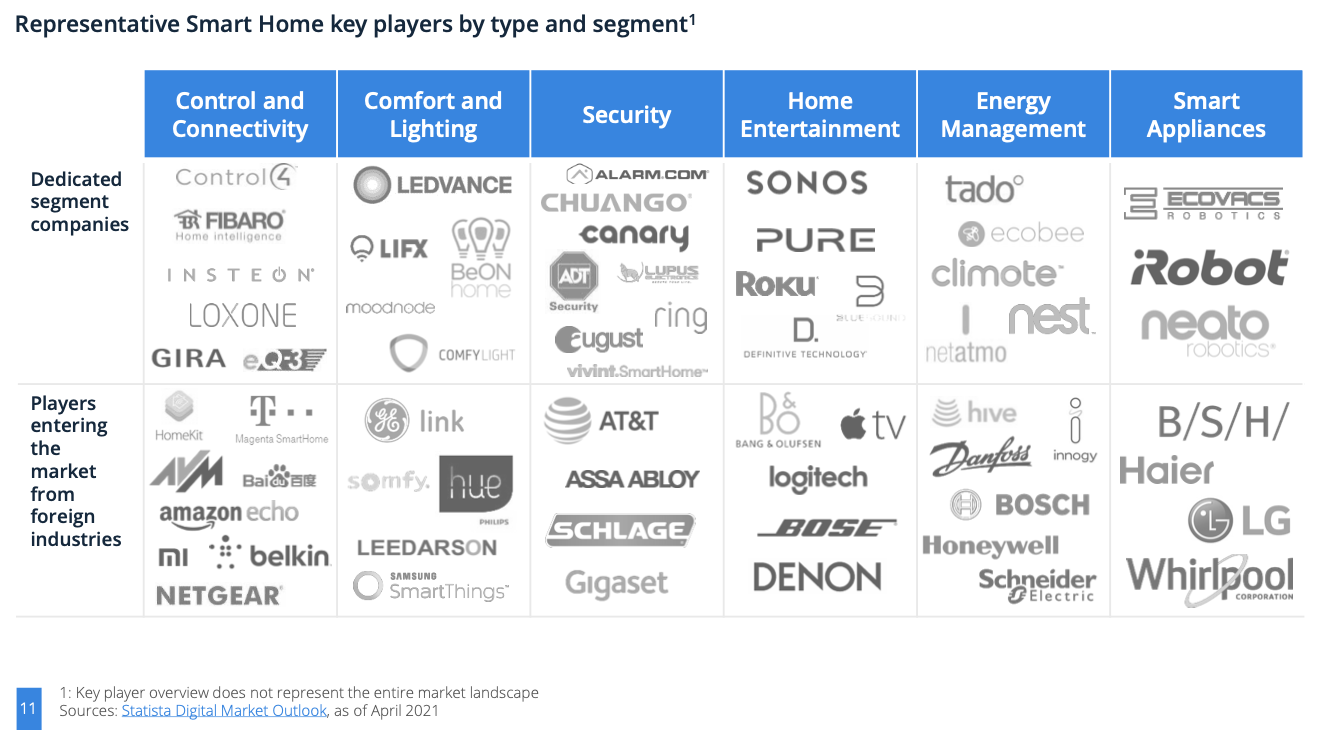
\includegraphics[width=15cm,height=10cm,keepaspectratio]{images/keyplayers.png}
            \caption{Übersicht der repräsentativen Schlüsselanbieter \cite{statista2021}} 
            \label{pic:landscape}
        \end{figure}
        \\
        Die Übersicht deckt jedoch nicht alle Anbieter ab und spezialisiert sich in diesem Fall auf die bekanntesten und die am 
        Markt etablierten. 
        \\
        \linebreak
        Laut den von Statista veröffentlichten Daten war die USA mit einem Umsatz von 28,86 Milliarden US-Dollar der größte 
        \acl{SH} Markt im Jahr 2021, wogegen Deutschland eine Umsatz von 6,59 Milliarden US-Dollar erzielte. Zu berücksichtigen sind 
        dabei jedoch die Demographische Lage als auch die Bevölkerungsdichte. Diese Aufstellung steht in keinem direkten Vergleich und 
        dient lediglich zur Veranschaulichung und zur Unterscheidung der Marktanteile. Deutlich wird dabei jedoch, dass das 
        Marktwachstum prozentual ähnlich ansteigt. 
        \\
        \linebreak
        Der Markt-Prognose in Abbildung (\ref{pic:revenue}) ist zu entnehmen, dass bis 2026 sich der Umsatz nahezu verdoppeln 
        wird. Der Darstellung (\ref{pic:globalmarket}) der einzelnen Segmente kann entnommen werden, dass der Weltmarkt von 
        2021 bis 2026 um ca. 100 Prozent zunimmt. Die Zeitspanne von 2019 bis 2026 stellt einen durchschnittlichen Zuwachs von 
        17,4 Prozent dar. Anhand der Prognose und des Berichts von Statista ist deutlich zu sehen, dass der \acl{SH} Markt in 
        den nächsten Jahren erheblich wachsen wird. Prognostiziert ist ein globaler Marktwert bei ca. 207,8 Milliarden 
        US-Dollar bis 2026.
        \begin{figure}[hbt!]
            \centering
            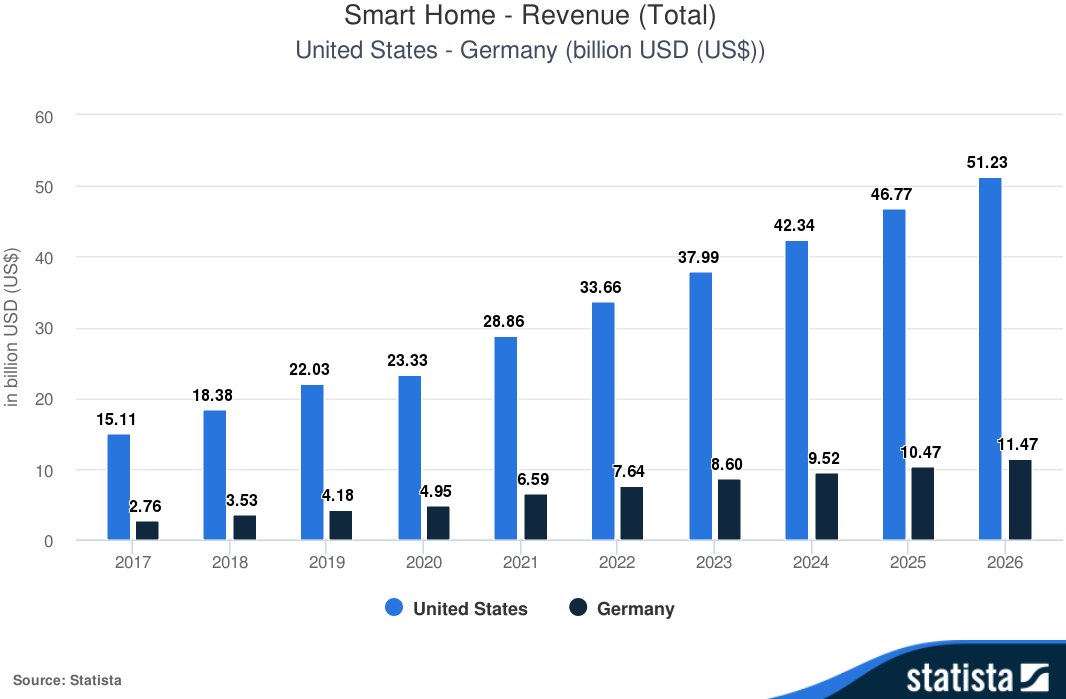
\includegraphics[width=15cm,height=9.25cm,keepaspectratio]{images/Statista-Outlook-Smart-Home---Revenue-Total-United-States---Germany-billion-USD-US.png}
            \caption{Umsatz-Prognose von Deutschland und den USA \cite{statista2021}} 
            \label{pic:revenue}
        \end{figure}
        \\
        \begin{figure}[hbt!]
            \centering
            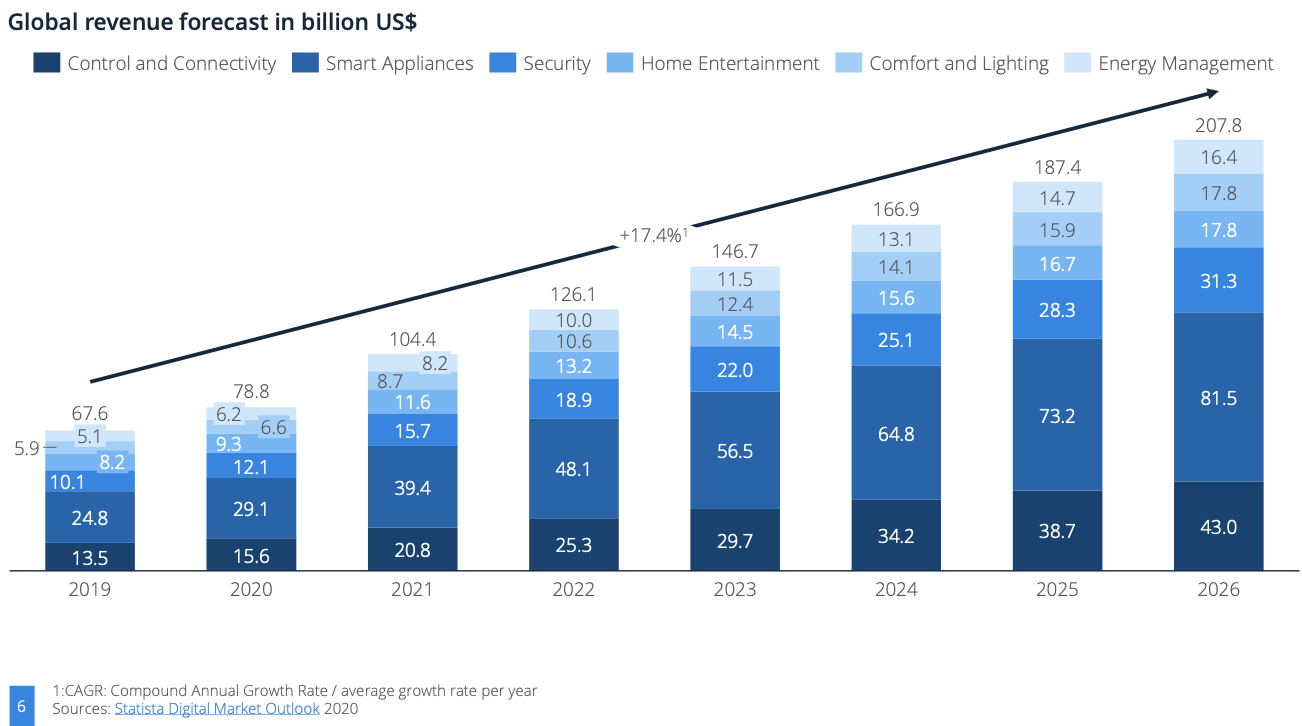
\includegraphics[width=15cm,height=10cm,keepaspectratio]{images/global_Worth_smart-home.png}
            \caption{Globaler Smart Home Marktwert \cite{statista2021}} 
            \label{pic:globalmarket}
        \end{figure}
        \pagebreak 
    \subsection*{Schlüsseltechnologien und Barrieren}
        Unter den Schlüsseltechnologien im \acl{SH} sind Komponenten zu verstehen, die den Gedanken eines intelligenten 
        Wohnraumes und Gebäudes forcieren. Dazu zählen unter anderem die Spracherkennung, die bei Sprachassistenten, 
        darunter bspw. Amazon Alexa, Apple HomePod (Siri) und dem Google Nest, eingesetzt wird, sowie \ac{AI} und \ac{KI} 
        zur Analyse, Auswertung und Optimierung von Verhaltensmustern und weiteren Analysezwecken \cite{statista2021}. 
        Obwohl die Spracherkennung das Wachstum des Marktes ankurbelt, werden die herkömmlichen Interaktionsmöglichkeiten, 
        z.B. die Kontrolle über Berührung durch Touch-Displays,
        weiter bestehen und weiterhin eine wichtige Art des Gerätezugriffs darstellen \cite{all-electronics2022}. 
        Mit dem Einsatz von \acs{KI} und \acs{AI} werden Prozesse noch autonomer und können den Komfort aus den Analysen je 
        nach Bedürfnis individuell gestalten. Zu berücksichtigen ist dabei jedoch die dafür geeigneten Anwendungsfälle und 
        die Bereitschaft der Nutzer, in wie fern diese das Analysieren von Verhaltensmustern akzeptieren und zulassen. 
            
        \subsubsection*{Fehlender Interoperabilität}
            Die Kommunikation von \acl{SH} Geräten findet über drahtlose Netzwerke auf Brandbreiten statt, die oft nicht 
            miteinander kompatibel sind. Der hauptsächliche Grund dafür ist, dass Unternehmen ein Protokoll für einen 
            bestimmten Zweck entwickeln und dieses darauf abgestimmt ist den Anwendungsfall abzudecken und um eine 
            Markteintrittsbarriere zu schaffen, sodass der Wechsel zwischen Anbietern erschwert wird \cite{statista2021}. 
            Die damit einhergehende Schwachstelle eines \acl{SH} ist, dass die Geräte mit den bereits entwickelten 
            Protokollen genutzt werden. So ist die Kommunikation über verschiedene Protokollen nicht vorgesehen. Dadurch 
            entsteht die fehlende Interoperabilität, die der Anwender jedoch für eine \acl{SH} Lösung ansieht und auch 
            als äußerst sinnvoll betrachtet. Die Einführung von Bluetooth LE Mesh ist eine aktuelle Entwicklung, um der 
            Herausforderung der Bewältigung der Interoperabilität einen Schritt näher zu kommen. Dennoch muss der 
            Anwender prüfen, welche Geräte miteinander kompatibel sind \cite{statista2021}. Bei cloudbasierten 
            Sprachdiensten muss ebenso die Kompatibilität geprüft werden. 
            Dadurch wird dem Nutzer neben der Ungewissheit der Datensicherheit und der Privatsphäre ein weiterer Aspekt 
            geliefert, der die Nutzung von \acl{SH} Lösungen für bestimmte Anwendergruppen immer noch in Frage stellt.
            \\ 
            \linebreak
            Derzeit häufig verwendete Protokolle sind unter anderem Bluetooth, \ac{WLAN} (WiFi), KNX, ZigBee, Z-Wave, 
            MQTT und weitere (siehe \ref{tab:protocolsSH}). Um Beispielsweise mit ZigBee über \acs{MQTT} kommunizieren zu 
            können, gibt es ein Framework, welches die Interoperabilität der beiden Protokolle ermöglicht. Dies ist das 
            sogenannte \textit{ZigBee2MQTT} Framework\footnote{Erschafft eine Brücke zwischen ZigBEE und MQTT. \url{https://www.zigbee2mqtt.io/} Abgerufen am 23.05.2022}.
\pagebreak
\section{Zielgruppenanalyse}
\label{sec:zielgruppenanalyse}
    Zur Analyse der Zielgruppen, die \acl{SH} Lösungen nutzen, bzw. die als Anwender des im Rahmen dieser Arbeit 
    entstehenden Konzeptes gelten, erfolgt in diesem Abschnitt eine Zielgruppenanalyse. Hierbei wird zwischen 
    zwei Gruppen stark differenziert. Zum einen erfolgt die Benutzer-Analyse, die aufzeigt, welche Zielgruppen 
    im allgemeinen Kontext \acl{SH} adressiert werden, und zum anderen die Anwender-Analyse, die sich 
    konkret der Zielgruppe widmet, die in dieser Arbeit adressiert wird. 

    \subsection{Ziel der Zielgruppenanalyse}
        %was soll damit erzielt werden?
        Ziel einer Zielgruppenanalyse\footnote{Beschreibung der Zielgruppenanalyse und mögliche Durchführungsschritte. \url{https://www.eology.net/magazine/target-group-analysis} Abgerufen am 24.05.2022.} 
        ist die Identifizierung der Personengruppen, die als potentielle Nutzer eines Produktes 
        oder eines Marktsegmentes gelten. Diese Methodik ist ein relevantes Werkzeug in der Produktkonzeption und -entwicklung 
        als auch in der Marktforschung. Maßnahmen und Anforderungen können aus der Zielgruppenanalyse abgeleitet und 
        erarbeitet werden. 
        \\
        Ein Weiteres Ziel ist das bessere Kennenlernen der Zielgruppe, um dadurch deren Bedürfnisse und Interessen 
        genauer zu identifizieren und zu betrachten. 
    
        \subsection{Benutzer-Zielgruppe}
        % Smart Home - Deutschland. Zugriff: 11. Mai 2022. https://de.statista.com/outlook/dmo/smart-home/deutschland
            Die in der Marktanalyse (\ref{sec:marktanalyse}) identifizierten Segmente werden in der Abbildung 
            (\ref{pic:segments}) nochmals aufgegriffen. Hierbei wird in der repräsentativen Statistik und Prognose der 
            Statista GmbH die Nutzung des jeweiligen Segments veranschaulicht. Der Fokus dieser Prognose liegt 
            auf der verstärkten Vertretung eines Segments in einem \acl{SH} in Deutschland. Die derzeit am meisten eingesetzten 
            Segmente sind \textit{Vernetzung und Steuerung} (rot gekennzeichnet) und \textit{Komfort und Licht} 
            (gelb gekennzeichnet). Das am wenigsten genutzt Segment stellt die \textit{Gebäudesicherheit} 
            (schwarz gekennzeichnet) in der Prognose dar. Im Jahr 2021 lag die Nutzung von Geräten des Segments \textit{Vernetzung 
            und Steuerung} bei 6,6 Millionen Nutzer, dicht gefolgt von dem Segment \textit{Komfort und Licht} mit 
            6,5 Millionen Nutzer. Dagegen liegt das Segment \textit{Home Entertainment} im Jahr 2021 bei 3,8 Millionen Nutzer.
            \\
            \linebreak
            Die bis 2026 veröffentlichte Prognose gibt vor, dass die jeweiligen Segmente stark zunehmen %werden 
            und sich jeweils vervierfachen.  
            \pagebreak
            \begin{figure}[hbt!]
                \centering
                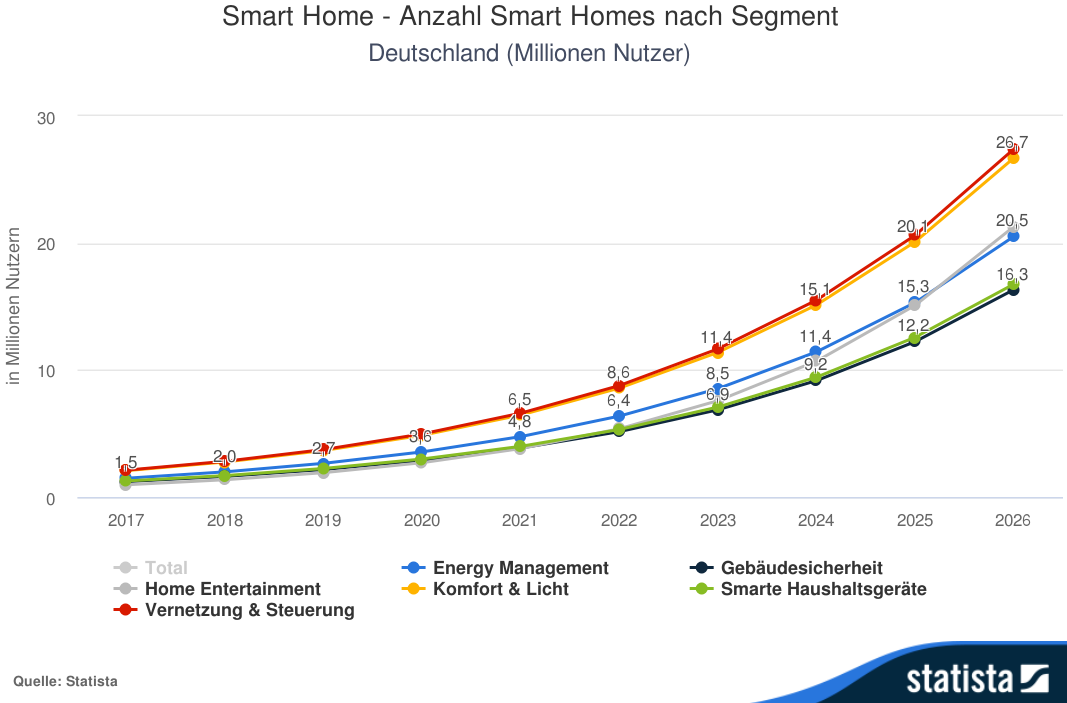
\includegraphics[width=15cm,height=10cm,keepaspectratio]{images/Statista-Outlook-Smart-Home---Anzahl-Smart-Homes-nach-Segment-Deutschland-Millionen-Nutzer.png}
                \caption{Anzahl Smart Home nach Segment \cite{statista2021}} 
                \label{pic:segments}
            \end{figure}
            \\
            Das Resümee der Prognose zeigt, dass eine breitere Masse an Personen bereits Komponenten der Segmente 
            \textit{Vernetzung und Steuerung} und \textit{Komfort und Licht} nutzen.
            \\
            \linebreak
            Im Hinblick auf die demographischen Statistiken wird in der Zielgruppenanalyse deutlich, welche Gesellschaftsschicht 
            im Jahr 2021 am stärksten vertreten ist. Diese erstreckt sich über eine Altersspanne von 25 bis 54 Jahren. 
            Wobei der Abbildung (\ref{pic:ageSH}) zu entnehmen ist, dass der Schwerpunkte im Alter zwischen 45 und 54 Jahren 
            mit 22,7 Prozent. Die Balance nach Geschlecht liegt bei einem Anteil von 45,6 Prozent weiblichen Befragten und 
            54,4 Prozent männlichen Befragten, demnach eine geringe Ungleichheit. Die Auswertung nach Einkommen zeigt, dass 
            35,4 Prozent der Befragten mit mittlerem Einkommen Komponenten eines \acl{SH} nutzen, dicht gefolgt von 
            Personen mit hohem Einkommen, diese liegen bei 34,9 Prozent. 
            \\
            \linebreak
            Demzufolge ist eine große Masse adressiert, die jedoch nach den Segmenten (siehe Abbildung \ref{pic:segments}) 
            wiederum eingeschränkt werden kann.
            \begin{figure}[hbt!]
                \centering
                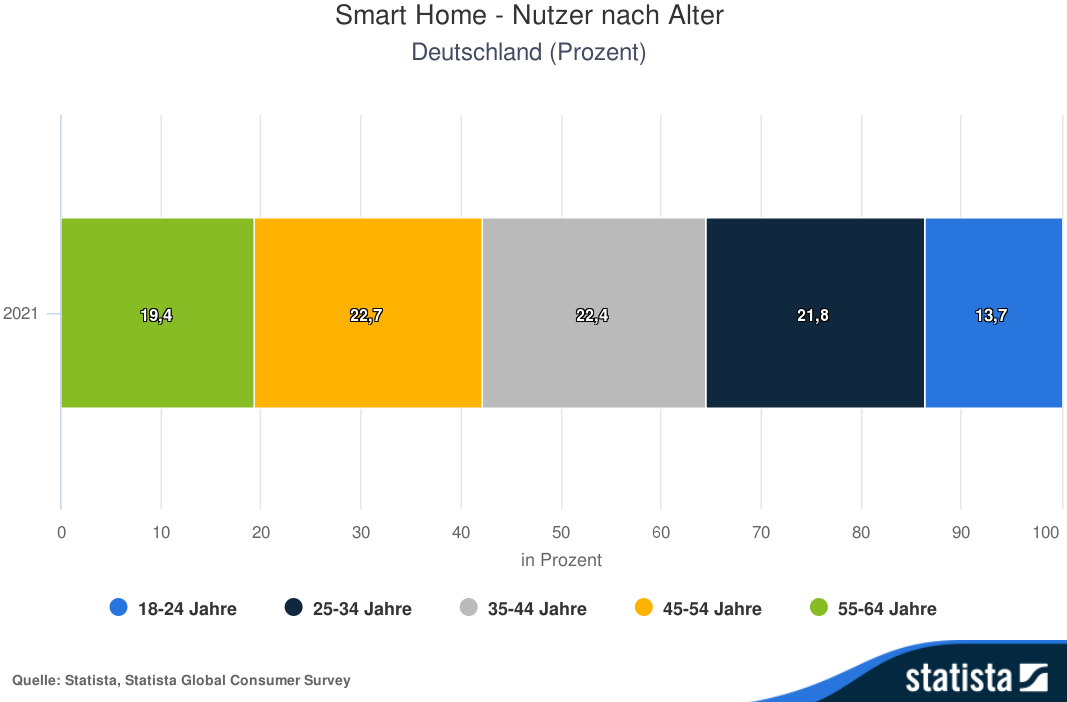
\includegraphics[width=15cm,height=10cm,keepaspectratio]{images/Statista-Outlook-Smart-Home---Nutzer-nach-Alter-Deutschland-Prozent.png}
                \caption{Smart Home Nutzer nach Alter \cite{statista2021}} 
                \label{pic:ageSH}
            \end{figure}
            Die aufgeführten Statistiken und Prognosen zeigen den Markt rundum \acl{SH} auf und welches Potential für die 
            nächsten Jahre prognostiziert wird. Im Hinblick auf die Zielgruppe lässt sich sagen, dass eine breite Masse 
            fokussiert werden kann, die jeweils unterschiedliche Voraussetzungen und Bedürfnisse haben. Diese Analyse zeigt 
            jedoch den gesamten Markt auf, um einen Einblick zu gewährleisten, wie stark \acl{SH} momentan in Deutschland, den 
            Vereinigten Staaten (USA) und dem Rest der Welt vertreten ist. Um einen konkreteren Einblick 
            zu gelangen, wird in nachfolgendem Abschnitt auf die Zielgruppe der Anwender, die in dieser Arbeit fokussiert werden, 
            eingegangen. 

        \subsection{Anwender-Zielgruppe}
            Der Benutzergruppe wird die Anwenderzielgruppe gegenübergestellt, diese können jedoch ebenso Benutzer der Anwendung 
            werden. Im Umkehrschluss ist ein gewisses Maß an \acs{IT}-Affinität vorausgesetzt, sodass Benutzer nicht gleich Anwender 
            sind. Es wird eine grundlegende Kenntnis der Programmierung erfordert, im Rahmen dieser Arbeit der Umgang mit der 
            Programmiersprache Java. 
            \\
            Im Fokus steht der Softwareentwickler als Anwender, welcher das System betreibt und auf die individuellen Bedürfnisse 
            anpasst. 
            %Die eigentliche Zielgruppe, die
        %Softwareentwickler, die das System betreiben und für ihre Bedürfnisse anpassen.

\section{Use Cases}
\label{sec:usecases}
    Für die Erhebung und Ausarbeitung aller Anforderungen an das System, werden Anwendungsfälle, sogenannte Use Cases, 
    definiert, bewertet und auf ihre Funktionalität geprüft und dokumentiert. Zum besseren Verständnis wird auf diese in den 
    folgenden Abschnitten eingegangen. 
\subsection{Check in mit Temi}
\subsection{Notfallevakuierung mit Temi}
\section{Experten Interview}
\label{sec:experteninterviewReqirements}
    Zur Analyse und Erhebung von Anforderungen, die sich an das System richten, werden Experten Interviews durchgeführt. 
    Dabei wird sich, wie in dem Abschnitt (\ref{subsec:experteninterview}) beschrieben, an dem unstrukturierten Ansatz der 
    Führung eines solchen Interviews orientiert \cite{robson2002real}. Infolgedessen werden keine konkreten offenen oder 
    geschlossenen Fragen gestellt. Auf den Aufbau des Interviews wird in weiteren Schritten eingegangen. 
    \\
    Diese Interviews sind nicht repräsentativ, da sie im Rahmen dieser Arbeit keine große Masse abdecken. Diese dienen 
    lediglich der weiträumigeren Informationsgewinnung und dem Sammeln mehrerer Meinungsbilder, um aus allen Ideen, 
    Gedankenanstößen und Meinungen ein objektives Ergebnis und viele Anforderungen zu erhalten. 
    %Die Experten Interviews sind eine Möglichkeit, die Anforderungen zu erfassen, die durch die Entwicklung des Systems 
    %nicht durch eine einfache Marktanalyse erfasst werden konnten. Diese Interviews sind nicht repräsentativ und dienen lediglich 
    %der weiträumigeren Informationsgewinnung.
\subsection{Ziele des Experten Interviews}
    % Diese helfen dabei, mehrere Sichten, Meinungen und Erfahrungen einzuholen, um ein 

\subsection{Aufbau des Experten Interviews}
\subsection{Zusammenfassung der Experten Interviews}
    % Aus den Interviews ergaben sich Anforderungen, die in die Konzeption mit einfließen. Diese werden im folgenden 
    % Abschnitt thematisiert.
\section{Anforderungen}

\chapter{Konzeption}
\label{chap:konzept}
    In diesem Kapitel wird das erarbeitete Konzept dieser Arbeit dargelegt. Basierend auf den 
    Anforderungen, die aus den Anwendungsfällen, Experteninterviews und der Zielgruppenanalyse 
    erhoben wurden, werden die daraus generierten Überlegungen und Entscheidungen transparent 
    dargestellt. Durch die bereits erfolgten Schritte der Anforderungsanalyse (\ref{chap:anforderungsanalyse})
    sind erste Aufgaben der Konzeption abgeschlossen. 
    \\
    Zu Anfang des Kapitels wird das allgemeine Ziel eines Konzeptes erläutert. Anschließend 
    wird auf das Anwendungsumfeld des Systems, engl. Framework, (\ref{sec:anwendungsumfeld}) eingegangen. 
    % die abzudeckenden Funktionalitäten (\ref{sec:konzeptfunktionalitaet}), die 
    %aus den Anforderungen ermittelt wurden, eingegangen. 
    Darauf folgend wird anhand den 
    zugrundeliegenden Informationen das Architekturkonzept (\ref{sec:architekturkonzept}), sowie das 
    Softwarekonzept (\ref{sec:softwarekonzept}) erläutert. Des Weiteren werden die Hintergründe der 
    Wahl des Frameworks (\ref{sec:frameworkauswahl}) aufgezeigt. %Abschließend wird das konzipierte 
    % und prototypische Datenmodell \ref{sec:...} dargelegt. 

\section{Ziel der Konzeption}
\label{sec:konzeptziele}
    Das Ziel einer Konzeption ist die Veranschaulichung von abstrakten Ideen, geistiger Entwürfe und Leitideen. 
    Hierbei werden aus den zugrundeliegenden Problemstellungen, Szenarien und Anforderungen Entwürfe und 
    Lösungsmöglichkeiten erarbeitet und identifiziert. Diese helfen bei der Aufstellung von notwendigen Schritten 
    und dienen als Grundlage zur Untermauerung und Darlegung von Entscheidungen. Somit wird Dritten der Kontext, die 
    Domäne und das zu lösende Problem, bzw. die Lösung dargestellt. 
    \\
    \linebreak
    Im Rahmen dieser Arbeit ist das Ziel des Konzeptes die Veranschaulichung der Entscheidungsfindung zur Lösung des vorliegenden 
    Sachverhaltes. Das Konzept 
    erarbeitet eine Lösung zur Implementierung einer Anwendung zur Koordination von Regeln und Prozessen innerhalb eines 
    Firmenbüros. Hierbei wird der allgemeine Aufbau der Architektur skizziert und demonstriert, wie eine solche Lösung aussehen kann. 
    Unter Berücksichtigung der Forschungsfrage (siehe Abschnitt \ref{sec:forschungsfragen}) wird eine Möglichkeit offengelegt, mit der 
    ein Softwareentwickler neue Regeln entwickeln und dem System hinzufügen kann, ohne ein weiteres zu erlernendes Framework zu verwenden. 
    Dabei sollen die notwendigen Schritte und Interaktionen formalisiert und für den Entwickler vereinfacht werden. Mit der 
    Definition der Zielsetzung der Arbeit (siehe Abschnitt\ref{sec:zielsetzung}) wird die Abgrenzung deutlich. In folgender 
    Darlegung des Konzeptes wird nochmals konkreter auf den Kontext als auch auf die Intension eingegangen. 
    % Das Ziel des Konzeptes ist es, dem Entwickler den Aufwand zur Erweiterung des Systems zu minimieren durch weitere 
    % Regeln und Abdeckung von Anwendungsfällen (Use Cases) und eine Struktur vorgeben. (ToDo's, Flexibilität in der 
    % Umsetzung (nicht wie Home Assistant und openHAB eher eingeschränkt)) 

%\section{Abzudeckende Funktionalitäten}
%\label{sec:konzeptfunktionalitaet}
    % Was soll der Entwickler machen können? 
    % Welche Grundlagen braucht er, um eine Regel implementieren zu können?
    % Welche Funktionen müssen gegeben sein, um die Struktur vorzugeben? 
    % Reicht ein Hinweis weöche Stellen angepackt werden müssen, um eine Regel hinzuzufügen? 
    
    %%%%%%%%%%%%%%%%%%%%%%%%%%%%%%%%%%%%%%%%%%%%%%%%%%%%%%%%%%%%%

    % ZIEL DES KONZEPTES: Ein Framework für Entwickler bereitzustellen, welches die Mächtigkeit für den Entwickler offen lässt, nicht einschränkt 
    % und dennoch Konfiguration und Ausführung umsetzt. Der Entwickler muss lediglich den Zustandsraum, die MQTT-Topics und die Regeln definieren.
    % Der Entwickler bekommt ein Framework in die Hand, welches die Umsetzung von Prozessen in einem smarten Büro ermöglicht. Das Framework kümmert sich um die 
    % Organisation und die Ausführung der Regeln. Die Richtigkeit der Regeln und des Zustandsraumes muss der Entwickler sicherstellen. 
    % Die Kommunikation über MQTT ist nur eine Möglichkeit. Des Setup wird wegabstrahiert 

    %%%%%%%%%%%%%%%%%%%%%%%%%%%%%%%%%%%%%%%%%%%%%%%%%%%%%%%%%%%%%

\section{Anwendungsumfeld}
\label{sec:anwendungsumfeld}
    Grundsätzlich ist der Einsatzort des Frameworks variabel, da die eigentliche Implementierung und Nutzung der Regeln und Prozesse stark 
    abhängig von den Anwendern ist. Dadurch kann sowohl in privatem \acl{SH} Umfeld als auch in Büroräumen eine solche Instanz mittels dem 
    Framework erstellt werden. Basierend auf den vorangestellten Tätigkeiten, darunter die Anforderungsanalyse und die Eingrenzung auf den 
    Einsatz im Smart Office, liegt der Schwerpunkt auf dem Einsatz in einem smarten Büro. 

\section{Architekturkonzept}
\label{sec:architekturkonzept}
    % Es wird alles abgebildet über einen Zustandsraum, der sich aus den Dingen (Gegenständen) und Zuständen der Anwendung ergibt.
    % Der Zustandsraum wird verändert, wenn eine Aktion durchgeführt wird, bzw. durch eine Trigger angestoßen. 
    % Bzw. speichert den aktuellen Zustand des Gegenstandes 
    % (lightBulb = true/false, personOnDoor = null/Mikka, booking = stringBooking, temiAktive = true/false, 
    % temiPosition = stringKoordinates)
    % Zustandsraum muss von dem Entwickler definiert werden. 
    % MQTT Broker über Home Assistant, bzw. losgelöster Broker
    % Anbindung von APIs auch Entwickler-Sache. Kann ich das vereinfachen, sodass die Integration einfacher wird?

    \subsection{Überlegungen, Anstöße und Herausforderungen}
    % Regeln über Thread abbilden? Ja, Nein? - Nein, wieso? Da Durch die MQTT Message mehrere Regeln ausgeführt 
    %werden können. -> Lediglich den Zustand der Komponenten locken.
    % KEIN THREAD (wird schon abgebildet durch die Services und die Auslöser durch MQTT), Falls eine Komponente 
    %  doppelt beansprucht wird, ist der Zustand der Komponenten zu locken und ein 
    % Thread.sleep einzurichten. Abfrage, ob der Wert, bzw. die Komponente wieder freigegeben wurde. 

    % Zustandsraum -> Abbildung aller notwendigen Komponenten 
    % Bei Bearbeitung einer Regeln die Komponenten Locken, sodass nur die einzelne Komponenten (deren Zustand) gelockt ist 
    % und nicht der ganze Zustandsraum, somit können mehrere Komponenten und Aktionen ausführen zu können. 

    %Was brauche ich für Funktionen und Werte in einer Regel?

    % Ein Zustandsraum (Objekt) für alles oder ein Globales, welches die die Komponenten enthält? - Begründung für die Auswahl.
    
    \subsection{Schnittstellen}
        % Kommunikation mit API's je nach Use Case und Gebrauch zur Datenabfrage
    
    \subsection{Datenbanken}
        % Datenbanken je nach Use Case und Gebrauch zur Datenabfrage

\section{Softwarekonzept}
\label{sec:softwarekonzept}

\section{Auswahl des Frameworks}
\label{sec:frameworkauswahl}
    Im Bereich der Java-Entwicklung gibt es mittlerweile viele Möglichkeiten, um Applikationen, Anwendungen und Frameworks 
    zu entwickeln, die unterschiedliche Präferenzen und Einsatzmöglichkeiten bieten. Dadurch sind, auf den Einsatzbereich bezogen, 
    Vor- und Nachteile im Vergleich ähnlicher Systeme nicht auszuschließen. Eine kleine Auswahl an Systemen wurde getestet und auf deren 
    Brauchbarkeit analysiert und evaluiert. Für diese Evaluation wurden Kriterien ausgearbeitet, mit der die Auswahl des Frameworks 
    eingeschränkt und nach Möglichkeit das passende ergeben soll. Diese sind nach ihrer Relevanz aufgelistet: 
    \begin{enumerate}
        \item Freiheiten bei der Nutzung (Anwendung und Gewährleistung von Entwurfsmustern).
        \item Nutzung und Bereitstellung von Bibliotheken (Libraries).
        \item Bereitstellung einer Plattform (Full Stack).
        \item Aktive Community und stetige Weiterentwicklung des Systems.
        \item Nutzung des Frameworks in bereits bestehenden Projekten im Bereich Smart Home.
        \item Open Source-Projekt, um Flexibilität und weitestgehende Unabhängigkeit zu gewährleisten.
        \item Ausschluss von Frameworks, die ausschließlich für die Web-Entwicklung gedacht sind.
    \end{enumerate}  
    Aufgrund der Vielzahl an Frameworks war es im Rahmen dieser Arbeit nicht möglich, alle vorhandenen und in Betracht 
    gezogenen Systeme detailliert aufzuführen. Lediglich die engere Auswahl wird aufgegriffen. 
    Nach ausführlicher Recherche und unter Berücksichtigung von Frameworks, wie bspw. Grails, Quarkus, Blade, und Play, wurden 
    schließlich genau zwei Systeme gegenübergestellt, die die vorangestellten Kriterien in Gänze erfüllen. Viele in Betracht gezogenen Frameworks 
    finden überwiegend in der Web-Entwicklung Anwendung, bzw. basieren auf dem Spring Framework. Durch diese Erkenntnis wurden 
    viele Systeme nicht weiter berücksichtigt und betrachtet. Die beiden Kernsysteme, die ihren Einsatz und ihre Möglichkeiten rechtfertigen
    werden in den folgenden Abschnitten kurz erläutert.

    \subsection{OSGi}
    \label{subsec:osgiFramework}
        Das \ac{OSGI} Framework, welches in der openHAB Software eingesetzt wird, der \acs{OSGI}\footnote{Ursprung der OSGi Plattform. \url{https://www.osgi.org/about/} Abgerufen am 19.06.2022} 
        Alliance klassifiziert eine dynamische Softwareplattform, mit der die Modularisierung und Verwaltung von Applikationen und 
        den dazugehörigen Diensten mittels Komponentenmodell realisiert werden kann \cite{funke2009}. Bekannte Produkte, die auf der 
        \acs{OSGI} Plattform laufen, sind neben openHAB unter anderem die Entwicklungsumgebung Eclipse der Eclipse Foundation, Produkte 
        und Softwarelösungen von IBM, Oracle, Adobe und weitere. 
        \\
        Nennenswerte Eigenschaften und Vorteile der Software sind die Modularisierung und Versionierung, das zur Laufzeit organisierte 
        Abhängigkeitsmanagement, das Fernmanagement des laufenden Systems über sogenannte Management Agents und die Nutzung des 
        Serviceorientiert Programmiermodell. An dieser Stelle wird das Framework nicht technisch vertieft. Die Funktionsweise und die technisch 
        fundierte Erläuterung kann dem Buch \cite{osgibuch}, sowie der Dokumentation \cite{osgipraesentation} eines ausgearbeiteten Workshops entnommen werden. 
        Nachteile der Plattform ist zum einen der weniger breite Einsatz des Frameworks und die kleine Community. 
        Ebenso findet eine Weiterentwicklung der Plattform nur mäßig statt. 

    \subsection{Spring Boot}
    \label{subsec:springBootFramework}




\chapter{Umsetzung}
\label{chap:umsetzung}
    Im Rahmen einer prototypischen Implementierung wurde das im Kapitel Konzeption (\ref{chap:konzept}) geplante Systems 
    umgesetzt. Gegenstand dieses Kapitels wird es sein, Aspekte der Umsetzung widerzuspiegeln und konkret die Umsetzung eines  
    Anwendungsfalls darzulegen. Zusätzlich wird die Auswahl des dafür genutzten Frameworks aufgegriffen. 

\section{Auswahl des Frameworks}
\label{sec:frameworkauswahl}
    Im Bereich der Java-Entwicklung gibt es mittlerweile viele Möglichkeiten, um Applikationen, Anwendungen und Frameworks 
    zu entwickeln, die unterschiedliche Präferenzen und Einsatzmöglichkeiten bieten. Dadurch sind, auf den Einsatzbereich bezogen, 
    Vor- und Nachteile im Vergleich ähnlicher Systeme nicht auszuschließen. Eine kleine Auswahl an Systemen wurde getestet und auf deren 
    Brauchbarkeit analysiert und evaluiert. Für diese Evaluation wurden Kriterien ausgearbeitet, mit der die Auswahl des Frameworks 
    eingeschränkt und nach Möglichkeit das passende ergeben soll. Die Kriterien sind nach ihrer Relevanz aufgelistet: 
    \begin{enumerate}
        \item Freiheiten bei der Nutzung (Anwendung und Gewährleistung von Entwurfsmustern).
        \item Nutzung und Bereitstellung von Bibliotheken (Libraries).
        \item Bereitstellung einer Plattform (Full Stack).
        \item Aktive Community und stetige Weiterentwicklung des Systems.
        \item Nutzung des Frameworks in bereits bestehenden Projekten im Bereich Smart Home.
        \item Open Source-Projekt, um Flexibilität und weitestgehende Unabhängigkeit zu gewährleisten.
        \item Ausschluss von Frameworks, die ausschließlich für die Web-Entwicklung gedacht sind.
    \end{enumerate}  
    Aufgrund der Vielzahl an Frameworks war es im Rahmen dieser Arbeit nicht möglich, alle vorhandenen und in Betracht 
    gezogenen Systeme detailliert aufzuführen. Lediglich die engere Auswahl wird aufgegriffen. 
    Nach ausführlicher Recherche und unter Berücksichtigung von Frameworks, wie bspw. Grails, Quarkus, Blade, und Play, wurden 
    schließlich genau zwei Systeme genauer betrachtet, die die vorangestellten Kriterien in Gänze erfüllen. Viele in Betracht gezogenen Frameworks 
    finden überwiegend in der Web-Entwicklung Anwendung, bzw. basieren auf dem Spring Framework. Durch diese Erkenntnis wurden 
    viele Systeme nicht weiter berücksichtigt. Die beiden Kernsysteme, die ihren Einsatz und ihre Möglichkeiten rechtfertigen
    werden in den folgenden Abschnitten kurz erläutert.

    \subsection{OSGi}
    \label{subsec:osgiFramework}
        Das \ac{OSGI} Framework der \acs{OSGI}\footnote{Ursprung der OSGi Plattform. \url{https://www.osgi.org/about/} Abgerufen am 19.06.2022} 
        Alliance, welches in der openHAB Software eingesetzt wird, klassifiziert eine dynamische Softwareplattform, mit der die Modularisierung 
        und Verwaltung von Applikationen und den dazugehörigen Diensten mittels Komponentenmodell realisiert werden kann \cite{funke2009}. Bekannte 
        Produkte, die auf der \acs{OSGI} Plattform laufen, sind neben openHAB unter anderem die Entwicklungsumgebung Eclipse der Eclipse 
        Foundation, Produkte und Softwarelösungen von IBM, Oracle, Adobe und weitere. 
        \\
        Nennenswerte Eigenschaften und Vorteile der Software sind die Modularisierung und Versionierung, das zur Laufzeit organisierte 
        Abhängigkeitsmanagement, das Fernmanagement des laufenden Systems über sogenannte Management Agents und die Nutzung des 
        Serviceorientierten Programmiermodells, \ac{SOA}\footnote{Erläuterung des SOA Modells. \url{https://www.ibm.com/cloud/learn/soa} Abgerufen am 20.06.2022}. 
        An dieser Stelle wird das Framework nicht technisch vertieft. Die Funktionsweise und die technisch 
        fundierte Erläuterung kann dem Buch \cite{osgibuch}, sowie der Dokumentation \cite{osgipraesentation} eines ausgearbeiteten Workshops entnommen werden. 
        Nachteile der Plattform sind zum einen der weniger breite Einsatz des Frameworks und zum anderen die kleine Community. 
        Ebenso findet eine Weiterentwicklung der Plattform nur mäßig statt. Dies hat zur Folge, dass die Erweiterung, bzw. die Entwicklung des darauf 
        aufbauenden Systems träge vonstattengeht. 
        %Wieso Spring Boot und nicht OSGi?
        %Wieso Java und nicht Python oder andere?

    \subsection{Spring}
    \label{subsec:springBootFramework}
    Spring\footnote{Open-Source-Framework Spring. \url{https://spring.io} Abgerufen am 02.07.2022} ist ein Open-Source-Framework, welches auf der Java-Plattform aufbaut. 
    Das Ziel von Spring selbst ist die Vereinfachung und Förderung von Programmierpraktiken in der Java- und Java EE Entwicklung. Mit einem breiten Spektrum an 
    Funktionalitäten bietet das Framework eine ganzheitliche Lösung zur Entwicklung von Applikationen, Anwendungen und Frameworks. Im Vordergrund dabei steht immer die 
    Entkopplung von Applikationskomponenten. Das Spring Framework wurde im März 2004 offiziell Freigegeben und wird seitdem stetig weiterentwickelt. 
    Initiator des Frameworks ist der Author und Softwareentwickler Rod Johnson. Das Framework, welches in dem Buch des Experten Rod Johnson erläutert wird, basiert auf 
    den folgenden Prinzipien \cite{johnson2004expert}: 
    \\
    \linebreak
    Dependency Injection ist ein sehr bekanntes Entwurfsmuster. Dabei werden die Abhängigkeiten eines Objektes zur Laufzeit reglementiert. Unter 
    Verwendung des Frameworks werden den Objekten die benötigten Objekte und Ressourcen zugewiesen. Dadurch müssen diese nicht selbst gesucht werden. 
    \\
    \linebreak
    Ein weiterer Punkt ist die aspektorientierte Programmierung, durch die der Entwickler technische Aspekte voneinander isolieren und den eigentlichen Programmcode 
    von Transaktionen oder anderen Faktoren freizuhalten. 
    \\
    \linebreak
    Das dritte Prinzip ist das Bereitstellen von Vorlagen zur Vereinfachung der Nutzung von Schnittstellen, sog. \acs{API}s. Dadurch wird ein POJO-basiertes Modell 
    möglich. Unter POJO, \textit{Plain Old Java Object}, ist ein ganz normales Objekt in Java zu verstehen. 
    \\
    \linebreak
    Zusammenfassend sind beide Frameworks dazu geeignet, um das Konzept der Steuerzentrale unterstützend zu realisieren. 
    Ein direkter Vergleich zwischen den Frameworks kann nicht gezogen werden, da die Funktionalitäten, bzw. die aus der Nutzung 
    profitablen Eigenschaften nicht vergleichbar sind. Während sich Spring auf die Unterstützung zur Erstellung von Applikationen konzentriert, 
    legt \acs{OSGI} den Mehrwert auf die Modularisierung durch Kontainerisierung. Durchaus ist eine Kombination aus beiden 
    Frameworks möglich, um Vorteile beider zu vereinen. Fundamental bietet Spring jedoch weitaus mehr Möglichkeiten und Unterstützungen 
    zur Entwicklung von Applikationen und Frameworks, weshalb es im Rahmen dieser Arbeit eingesetzt wird. Mit Spring Boot, welches auf Spring 
    aufbaut können auch \acl{MVC} Web-Architekturen und \acs{REST} \acs{API}s implementiert werden. So kann mit dieser Entscheidung 
    ein Vollumfängliches System erstellt werden. Unter zusätzlicher Verwendung von \acs{OSGI} wäre eine weiter Modularisierung und Kontainerisierung möglich. Dies 
    ist auch durch Spring mit Hilfe von Microservices in einer anderen Form realisierbar. 
    \\
    An der Stelle wird im Rahmen dieser Arbeit das Thema von Microservices und Kontainerisierung nicht weiter konkretisiert.
    \\
    \linebreak
    Die Entscheidung viel auf Spring, da dieses ein modernes und etabliertes Framework darstellt und die 
    Community erheblich größer ist, als die des \acs{OSGI} Frameworks. Hinzukommt, die Schaffung eines alternativen Ansatzes zu openHAB, da dieses System bereits 
    auf \acs{OSGI} aufbaut. 
    Dennoch unterscheidet sich die Steuerzentrale in den Funktionalitäten und Angeboten immens im Vergleich zu openHAB. Das System bietet weitaus mehr 
    Funktionalitäten, Erweiterungen und Ausprägungen. Lediglich kann zum Vergleich die Definition von Regeln herangezogen werden. 

\section{Implementierung}
\label{sec:implementation}

\subsection{Generische Programmierung} % Typisierung
% Erledigt! -> WICHTIG!!!: Verwendung der Typisierung, um dem Anwender die Möglichkeit der offenen Gestaltung des Zustandobjektes zu gewährleisten.
Eine entscheidende konzeptionelle Überlegung in Richtung des Zustandsraumes wird vorab erläutert, damit in 
folgenden Darstellungen klar zwischen der Objektdarstellung und der eigentlichen Repräsentation des Zustandes 
differenziert werden kann. 
\\
Mit dem Hintergrund, dass der Entwickler die volle Entscheidungsmacht über die Implementierung der 
Regeln, des Zustandsraumes und den dafür notwendigen Bedingungen beibehält, ist die Überlegung  
notwendig, wie mit einem Objekt gearbeitet werden kann, ohne dass es vorher bekannt ist. 
\\
\linebreak
Hierfür wird auf das Konzept der generischen Programmierung, sog. \textit{Generics}, gesetzt. Ein Synonym 
des Begriffs ist der parametrisierte Typ. Mit der Nutzung von Generics ist ein syntaktisches Mittel 
gegeben, mit dem Klassen und Methoden mit Typen parametrisiert werden können. Diese Typ-Variablen sind zum 
Zeitpunkt der Implementierung unbekannt und können beliebig definiert werden. Erst zur Laufzeit des Systems 
wird die Typ-Variable durch einen oder ggf. auch mehrere Typen ersetzt. Somit ist zur Laufzeit das 
Objekt, dessen Struktur, Methoden und Funktionen bekannt. Bei der Verwendung von generischen Typen gibt es 
Varianzfälle, die unterschiedliche Auswirkungen aufzeigen. Der für das Konzept relevante Fall ist der des 
einfachen Typ-Parameters. Weitere Varianzfälle werden in dieser Ausarbeitung nicht erläutert. 
\\
\linebreak
Ein konkretes Anwendungsbeispiel, wie es 
auch im Rahmen dieser Arbeit verwendet wird, sieht wie folgt aus:
\\
Das Framework arbeitet mit dem generischen Typ \textit{E}. Der Anwender soll nach der Implementierung der Klasse des Zustandsraumes das 
jeweilige Objekt dem Framework übergeben. So ist zur Laufzeit das konkrete Objekt bekannt. Zur Veranschaulichung dient folgendes Code-Beispiel:
\begin{lstlisting}[language=Java, frame=lines, xleftmargin=\parindent, style=algoBericht, label={code:generics}, captionpos=b, caption={Zustandsobjekt als Typ-Variable}]
public class LogicHub<E> {
private E state;
...
public E getState() {
return this.state();
}
...
}

public class Application {
private final LogicHub<InnovationLab> logicHub;

public static void main(String[] args) {
logicHub = LogicHub.getInstance();
logicHub.getState(); // -> returns the InnovationLab object 
                     // and it's values.
...
}
}
\end{lstlisting}
Mit den Java Generics ist eine leistungsstarke Ergänzung der Java-Sprache gegeben, da es die Arbeit des Programmierers einfacher und 
weniger Fehleranfällig macht. Zusätzlich wird durch die Generics die Typkorrektheit zur Kompilierzeit erzwungen und ermöglicht 
die Implementierung generischer Algorithmen, ohne für Anwendungen einen zusätzlichen Overhead zu verursachen. 
\\
Mit der Option des generischen Typs kann das Framework universell definiert und der Zustandsraum vom Anwender individuell implementiert werden.
\\
\linebreak
Die Darstellung des Zustandsobjektes wird als bereits bestehendes vorausgesetzt, um die folgenden Diagramme vollständig und sinngemäß wiederzugeben. 
Diese beschreiben jedoch zu keinem Zeitpunkt eine konkrete Struktur des Zustandsobjektes. 
\\
\linebreak
Im weiteren Verlauf wird der Aufbau des Frameworks erläutert, sowie die detaillierte Beschreibung der einzelnen Schichten und deren Funktionalität. 

\subsection{Parallelisierung}
\subsection{Inverse Transformation}

\subsection{Prototypische Implementierung des Anwendungsfalls - Check-in mit einem Service-Roboter}
%Erläuterung der Umsetzung des Anwendungsfalls (Mögliche Regeldefinition)
%-> Einbauen von Thread.sleeps um einen durchehenden Prozess zu durchlaufen oder 
% feingranulare Regeln, die immer wieder auf Rückmeldung über MQTT Topics warten und danach die Aktion auslösen


%\subsection{Aufbau der Architektur}
%\subsection{Einbindung der Funktionen abgeleitet von der Konzeption}
\section{Fazit der prototypischen Implementierung}
%\chapter{Ergebnis}
\label{chap:ergebnis}
\chapter{Evaluation}
\label{chap:evaluation}
In diesem Abschnitt wird das erzielte Ergebnis des erarbeiteten Konzeptes (siehe Kapitel \ref{chap:konzept}) und des 
Prototypen analysiert. Anhand von ausgewählten Forschungsmethoden werden die vorab identifizierten Anforderungen überprüft 
und evaluiert. Mithilfe der erhobenen Informationen wird zum Ende des Kapitels die Forschungsfrage sowie das
Ziel der Arbeit abschließend betrachtet. 

\section{Usability-Test}
\label{sec:usabilitytest}
    Im Rahmen der Evaluation wurde ein Usability-Test durchgeführt, um bestimmte, für die Nutzbarkeit aufgestellte Anforderungen zu 
    überprüfen.
    Das angestrebte Ziel und die Ergebnisse der Tests werden in dem folgenden Abschnitt erläutert:
    
    \subsection{Ziel des Usability-Tests}
        Anhand des Usability-Tests sind die Anforderungen zu prüfen, die den Bereich der Nutzbarkeit abdecken. 
        Hierfür werden die Anforderungen, die den Tabellen (\ref{tab:functionalRequirements}, \ref{tab:notfunctionalRequirements} und \ref{tab:furtherRequirements}) 
        zu entnehmen sind, betrachtet. Die dafür berücksichtigten Anforderungen sind konkret die Folgenden: NFA1, NFA2, NFA3 und NFA4 (siehe \ref{tab:notfunctionalRequirements}).
        \\
        Damit die Erfüllung der Anforderungen überprüfbar ist, wird ausgewählten Anwendern der Zielgruppe %im Rahmen der Nutzbarkeit 
        eine Aufgabe gestellt, mit der das Framework getestet wird und dabei die oben genannten Anforderungen genauestens betrachtet werden. 
        Ziel dabei ist die Überprüfung der Erfüllung der oben genannten Anforderungen an das System, bzw. Verbesserungen zu eruieren. 

    \subsection{Durchführung des Usability-Tests}
        Für die Durchführung der Tests wurde vorab eine Aufgabe erstellt. Diese 
        dient als Grundlage zur Identifizierung der Usability-Anforderungen. Der Aufbau und das Vorgehen der Testung wurde für jeden Teilnehmer 
        identisch gestaltet. Vor Beginn wurde der Kontext sowie das Framework und dessen Kernkomponenten, die Rahmenbedingungen und die Aufgabenstellung selbst erläutert. 
        Die Aufgabe war so zu erstellen, dass sie umgebungsunabhängig erfüllt werden konnte. 
        Da die Tests ausschließlich auf die Nutzung des Frameworks abzielten, war die Umgebung sowie die 
        Anbindung verfügbarer Geräte zu vernachlässigen. Voraussetzung war die Verfügbarkeit eines \acs{MQTT}-Brokers. 
        Durch die fehlende Anbindung von reellen Geräten wurden die ausgehenden 
        \acs{MQTT}-Nachrichten durch eine Simulation, konkret die eines Service-Roboters, verarbeitet. Eingehende Nachrichten 
        wurden simuliert, indem \acs{MQTT}-Nachrichten manuell veröffentlicht wurden. 
        \\
        Die von den Anwendern durchzuführende Aufgabe ist wie folgt definiert: 
        \\
        \linebreak
        Es soll ein Anwendungsfall implementiert werden, bei dem ein Service-Roboter einen Mitarbeiter oder Gast, der an der Tür steht, 
        empfangen und begrüßen soll. Die Eingangsbedingung ist die Authentifizierung über eine Kamera. Der ganze Vorgang wird simuliert, indem die \acs{MQTT}-Nachricht manuell erzeugt und ausgelöst wird. 
        Auch die Definition des \acs{MQTT}-Topics ist vorgegeben. 
        Danach soll über die Steuerzentrale eine Regel ausgeführt werden, anhand derer der simulierte 
        Service-Roboter gesteuert wird. Dafür sind folgende Anforderungen zu erfüllen: 
        \begin{itemize}
            \item Nach eingehendem Topic soll der Service-Roboter angesteuert und an die Tür geschickt werden. 
            (Die Ansteuerung des Service-Roboters erfolgt ebenso über \acs{MQTT}. Da in den meisten Fällen kein Roboter verfügbar ist, wird auch 
            diese Kommunikation mittels \acs{MQTT} simuliert.)
            \item Ist der Roboter an der Tür, soll er die Begrüßung starten. (Die folgende Interaktion wird im Rahmen des Test ebenso mittels der Simulation durchgeführt. 
            Wird die gesendete Nachricht über den Service-Roboter-\textit{Mock} auf der Konsole ausgegeben, so gilt die Aufgabe als erledigt.)
        \end{itemize}
        Für die Aufgabe sind folgende Punkte zu erfüllen:
        \begin{itemize}
            \item Die Kenntnis über \acs{MQTT}-Topics, die für die Kommunikation benötigt werden.
            \item Ein Zustandsraum, der alle benötigten Komponenten abbildet.
            \item Der Service-Roboter als Komponente, sodass dieser bei Ausführung einer Aufgabe für weitere Aufgaben gesperrt werden kann. 
            \item Der Auslöser, welcher durch ein \acs{MQTT} (PlugIn) abgebildet wird.
            \item Die Transformation der eingehenden \acs{MQTT}-Topics zu Zustandsänderungen, auf die Regeln ausgeführt werden sollen.
            \item Die Regel, die den Vorgang der Begrüßung und des Check-ins vorgibt.
        \end{itemize}
        Dem Anhang (siehe \ref{appendix:usabilitytestpaper}) ist das Dokument zur Durchführung des Usability-Test beigefügt. 
        \\
        \linebreak
        Nach dem Abschluss der Aufgabe wurden die Probanden um ihre Meinung mithilfe eines Fragebogens, der sich an dem \textit{System Usability Scale (SUS)} 
        Template orientiert, gebeten. Dieser Fragebogen ist ebenso dem Anhang (siehe \ref{appendix:usabilitytestpaper}) zu entnehmen. Auf die Auswertung wird in der 
        Zusammenfassung (\ref{subsec:usabilityFazit}) des Usability-Tests eingegangen. 

    \subsection{Fazit}
    \label{subsec:usabilityFazit}
        Der Usability-Test konnte erfolgreich durchgeführt werden.
        Das Ergebnis der quantitativen Forschung kann nicht als repräsentativ eingestuft werden, da es sich um eine kleine Auswahl an Experten handelt. Es zeigt dennoch eine Tendenz, 
        welche Anforderungen abgedeckt sind, bzw. welche Verbesserungspotentiale in dem Framework stecken.  
        Das Resultat der Aufgabe ähnelte sich bei den Probanden mit Ausnahme der Namensgebung der Attribute im Zustandsraum. 
        \\
        Folgender Auflistung ist der durchschnittliche Wert der Antworten zu entnehmen:
        \begin{enumerate}
            \item \textit{Ich denke, dass ich dieses System gerne öfter nutzen würde.} (80 Punkte)
            \item \textit{Ich fand das System unnötig komplex.} (8 Punkte)
            \item \textit{Ich fand das System einfach zu bedienen.} (76 Punkte)
            \item \textit{Ich denke, dass ich die Unterstützung einer technischen Person benötigen würde, um dieses System nutzen zu können.} (9 Punkte)
            \item \textit{Ich fand, dass die verschiedenen Funktionen in diesem System gut integriert waren.} (86 Punkte)
            \item \textit{Ich dachte, es gäbe zu viele Inkonsistenzen in diesem System.} (0 Punkte)
            \item \textit{Ich könnte mir vorstellen, dass die meisten Leute sehr schnell lernen würden, dieses System zu benutzen.} (89 Punkte)
            \item \textit{Ich fand das System sehr umständlich zu bedienen.} (5 Punkte)
            \item \textit{Ich fühlte mich sehr sicher mit dem System.} (76 Punkte)
            \item \textit{Ich musste viele Dinge lernen, bevor ich mit diesem System loslegen konnte.} (19 Punkte)
        \end{enumerate}
        Die Fragen aus dem \textit{SUS} (siehe Kapitel \ref{subsec:usabilitytests}) wurden verwendet und ins Deutsche übersetzt. 
        Im Rahmen der Bewertung, bei der 100 die volle Zustimmung und 0 die Ablehnung darstellt, ist das Ergebnis 
        sehr positiv und zeigt das Potential des Frameworks. 
        \\
        Nachdem der Test abgeschlossen und der Fragebogen beantwortet war, wurde die befragte Person abschließend noch interviewt, damit 
        Eindrücke über den Test hinaus gesammelt werden konnten. Diese Interviews werden im folgenden Abschnitt resümiert. 
        %1.: - 80 = 100, 75, 60, 80, 85 
        %2.: - 8 = 0, 15, 10, 10, 5 
        %3.: - 76 = 100, 80, 75, 75, 50 
        %4.: - 9 = 0, 5, 5, 10, 25 
        %5.: - 86 = 100, 90, 80, 85, 75 
        %6.: - 0 = 0, 0, 0, 0, 0 
        %7.: - 89 = 100, 100, 90, 85, 70
        %8.: - 5 = 0, 0, 5, 5, 15 
        %9.: - 76 = 85, 80, 75, 90, 50
        %10.: - 19 = 0, 15, 15, 20, 45 

\section{Experteninterview}
        Zur umfangreichen Informationsgewinnung wurde anschließend zu dem Usability-Test ein Interview mit dem jeweiligen Probanden 
        durchgeführt. Hierbei wurden sowohl die gesammelten Erkenntnisse und Erfahrungen während der Aufgabe erfragt sowie auf die Anforderungen 
        (siehe Kapitel \ref{sec:requirementsFinal}) eingegangen. Ein Teil der Probanden wurde dafür bereits 
        bei der Erhebung von Anforderungen befragt. Somit konnte sich ein Bild verschafft werden, wie die Anforderungen 
        umgesetzt, bzw. diese von den Experten empfunden wurden.
    
    \subsection{Ziele des Experteninterviews}
        Das Ziel des abschließenden Experteninterviews ist es, die Erfahrungswerte der Probanden zu sammeln, um diese den Anforderungen gegenüberzustellen. Bei 
        Experten, die bereits zu der Anforderungserhebung interviewt wurden, konnte konkret auf die Umsetzung der Kriterien und Anforderungen eingegangen werden. 
        Ebenso ist ein abschließendes Feedback wünschenswert, sowie ein Identifizieren der Herausforderungen für den Anwender und der eventuellen Schwachstellen 
        des Systems. 

    \subsection{Fazit}
        Das Experteninterview wurde, vergleichbar zu dem vorherigen Interview (siehe \ref{subsec:experteninterview}), mit einem semi-strukturierten Ansatz durchgeführt. 
        Anfangs wurde an den Fragebogen angeknüpft, um eine nachträgliche Zusammenfassung der Erkenntnisse jedes einzelnen zu erfahren. Sofern die Zusammenfassung bereits 
        die notwendigen Informationen enthielt, wurde ein unstrukturierter Ansatz verfolgt und ein offener Dialog geführt. War die Zusammenfassung jedoch nicht 
        aufschlussreich, so wurden anschließend konkret die 
        folgenden Fragen gestellt: 
        \begin{enumerate}
            \item \textit{„Wie ist Ihr erster Eindruck des Systems?“}
            \item \textit{„Gibt es aus Ihrer Sicht (Sicht des Anwenders) Mängel, die Ihnen die Nutzung des Frameworks erschweren?“}
            \item \textit{„Gab es Unklarheiten während der Anwendung des Frameworks? - Wenn ja, welche?“}
            \item \textit{„Haben Sie eine Idee oder Lösung, um diese Unklarheit zu beseitigen?“}
            \item \textit{„Gibt es allgemein Anregungen, bzw. Vorschläge für Verbesserungen?“}
            \item \textit{„Was gefällt Ihnen an dem Framework am meisten? - Was gefällt Ihnen nicht?“}
        \end{enumerate} 
        Rekapitulierend wurde ein aufschlussreiches und erfreuliches Ergebnis erzielt. Die Antworten gaben ein klares Meinungsbild von der Einfachheit der 
        Handhabung der formalisierten Interaktionen der Steuerzentrale wieder und bestätigen die Erfüllung des Ziels dieser Arbeit. 
        Aus Sicht des Anwenders gab es wenige Anmerkungen zum Aufbau des Frameworks. 
        \\
        Eine erwähnenswerte Anmerkung war folgende:
        \begin{quote}
            „Wenn man wenig bis keine Erfahrung mit der Java Entwicklung hat, gibt es klar die ein oder andere Wissenslücke, die zuerst beseitigt werden muss. 
            Durch die wenigen Handlungsschritte, die jedoch viel Interpretationsfreiheiten bieten, besonders bei der Regeldefinition, ist dies doch überschaubar. 
            Bekommt man dementsprechend eine Hilfestellung, bzw. eine detailliertes Beispiel an die Hand, so können kleinere Schritte und Anwendungsfälle 
            relativ schnell umgesetzt werden.“
        \end{quote}
        Ein Ergänzungs-, bzw. Verbesserungsvorschlag, der während eines Interviews erwähnt wurde, ist die Optimierung des Anlegens von sämtlichen Objekten. 
        Hierfür wurde vorgeschlagen, eine Art \textit{\ac{CLI}}, wie bspw. die von Angular\footnote{TypeSkript basiertes Web Application Framework. \url{https://angular.io/} Besucht am 05.08.2022}, 
        zu implementieren. Die Idee war Befehle über die Kommandozeile geben zu können, bspw. das Anlegen von Attributen im Zustandsobjekt, das Erzeugen leerer, bzw. mit den dafür 
        vorgesehenen Parameterwerten befüllter Transformationen, und das Erstellen eines leeren Regelkonstruktes. Dadurch würde der notwendige Code generiert und dem Entwickler zur Verfügung gestellt werden, wodurch dieser 
        sich ausschließlich um das Implementieren der Regeln kümmern muss. 
        \\
        \linebreak
        Abschließend lässt sich anmerken, dass mit der konkreten Anweisung, welcher Anwendungsfall umgesetzt werden soll, bzw. welche Randbedingungen 
        dafür gelten, schnell ein Ergebnis erzielt werden kann. 
        
\section{Evaluation der Anforderungen}
    Im Rahmen der Arbeit werden die Anforderungen (siehe Kapitel \ref{sec:requirementsFinal}) zum Abschluss anhand von dafür vorgesehenen Praktiken evaluiert. 
    Die Reihenfolge entspricht der tabellarischen Aufstellung der Anforderungen. Zuerst erfolgt die Abarbeitung der \textit{funktionalen Anforderungen}, 
    anschließend die der \textit{nicht funktionalen Anforderungen} und zum Ende hin die der \textit{zusätzlichen Anforderungen}. 
    
    \subsection*{Funktionale Anforderungen}
        Während der Konzeption und Entwicklung des Frameworks wurden die funktionalen Anforderungen (FA1 - FA6, siehe Tabelle \ref{tab:functionalRequirements}) 
        berücksichtigt. Sie stellen den wichtigsten Kernpunkt dar. Deren Erfüllung konnte durch die abschließenden 
        Experteninterviews identifiziert werden. Die Resonanz der Experten gab auch deutlich wieder, dass auf Grundlage der Anforderungen der Prototyp aufbaut. Die Struktur 
        des Regelobjektes (FA1) wird gegeben, indem eine Klasse von der Oberklasse erbt und diese erweitert. Umgesetzt wurde diese Anforderung mithilfe des 
        \textit{Template Method} Architekturmusters, auf das auch bereits in der Konzeption (siehe Kapitel \ref{chap:konzept}) eingegangen wurde. 
        \\
        \linebreak
        Die Anforderung (FA2) ist 
        umgesetzt, indem der Regel mit der \textit{ruleTrigger}-Methode ein Wert eines \textit{Enum Types}\footnote{Spezieller Datentyp. \url{https://docs.oracle.com/javase/tutorial/java/javaOO/enum.html} Besucht am 05.08.2022} 
        zugeordnet wird. Ein essentieller Teil des Frameworks ist der vom Anwender zu implementierende Zustandsraum, welcher über eine separate Klasse vorgegeben wird. Dadurch 
        ist auch die Anforderung (FA3) als umgesetzt anzusehen. Die Individualität der Implementierung des Zustandsraume ist durch die frameworkseitige Verwendung der 
        Java \textit{Generics} gegeben. Demzufolge arbeitet das Framework mit dem vom Entwickler übergebenen Klassenobjekt. 
        \\
        \linebreak
        Die Ausprägungen der Bedingungen zur Ausführung der Regelprozesse sind unverzichtbar. Sie müssen vom Anwender aufgestellt werden (FA4). Damit eine Aufstellung erfolgen kann, ist in der Regelklasse eine 
        Funktion gegeben, die das Implementieren der Bedingung erzwingt. 
        Die darauffolgende Forderung (FA5) ist prinzipiell gegeben, wird allerdings durch die Einschränkung im 
        Zustandsraum aktuell nicht als geeignet angesehen. Die Nutzung von Java \textit{Reflection}, bzw. die Umsetzung der inversen Transformation erschwert dies. Derzeit wird von der Komponenteneinbindung 
        in das Zustandsobjekt abgeraten. Das Erstellen von Komponenten ist dennoch möglich und kann im Regelkontext angewendet werden, sofern bestimmte Eigenschaften für eine Regel relevant sind. 
        \\
        \linebreak
        Der letzte Punkt (FA6) ist ebenso umgesetzt, da innerhalb der Regel bis auf die Voraussetzung der Implementierung der Regelbedingung sowie des -prozesses keine Einschränkungen bestehen. 
        Zusätzlich können bspw. sämtliche \acs{HTTP}-Abfragen getätigt werden. Im Falle des Use Cases "Check-in mit einem Service-Roboter" werden \acs{HTTP}-Abfragen ausgeführt, damit 
        Informationen der Büroplatzbuchungssoftware abgerufen werden können. 

    \subsection*{Nicht funktionale Anforderungen}
        Zur Überprüfung der \textit{nicht funktionalen Anforderungen} wurden Methoden für deren Überprüfung verwendet. Zusätzlich zu den 
        verifizierten \textit{User Stories} mittels der Usability-Tests konnten ebenso die aufgestellten Forderungen, die allgemein 
        die Benutzerfreundlichkeit (BF) umfassen, überprüft werden. Der durch die Experteninterviews aufgestellte Anspruch (NFA1) konnte 
        durch die Usability-Tests erfüllt werden, da die Probanden selten mehr als eine Aktion benötigten, um die bereits erstellte Regel 
        dem Framework zu übergeben. Grund dafür ist die Funktion der Steuerzentrale \textit{addRule(...)}. Der Anwender kann die Aufgabe der Funktion 
        schnell zuordnen und bekommt über die Entwicklungsumgebung die erwarteten Übergabeparameter mitgeteilt. 
        \\
        \linebreak 
        Im Rahmen des Usability-Tests waren alle Teilnehmer in der Lage eine Regel zu erstellen 
        und diese dem Regelwerk hinzuzufügen (NFA2). Ausgehend von dieser Anforderung wurden 
        während der Experteninterviews Anregungen angebracht, die gegebenenfalls eine weitere Vereinfachung für den Entwickler darstellen. 
        Diese werden im Ausblick (siehe Kapitel \ref{chap:ausblick}) aufgegriffen. 
        \\
        Durch die rein programmatische Anwendung des Frameworks kann der Entwickler zu jedem Zeitpunkt auf die Funktionen der Steuerzentrale zugreifen (NFA3). 
        Dies wurde ebenso von den Testteilnehmern im anschließenden Experteninterview bestätigt. Zum aktuellen Zeitpunkt sind die nutzbaren Funktionen sehr 
        überschaubar und decken die notwendigsten Funktion ab, darunter das Hinzufügen von Regeln, 
        Erstellen aller wesentlichen Objekte und Komponenten, Aufsetzen der erforderlichen \acs{MQTT}-Konfiguration, Ergänzen von Transformationen, Starten 
        des \acs{MQTT}-Clients und das Erweitern um zeitbasierte Regelauslöser. 
        \\
        \linebreak 
        Die Anforderung (NFA4) ist ebenso gegeben, da der Anwender sich 
        ausschließlich um die Definitionen der Regeln, der Transformationen und des Zustandsraumes kümmern muss. Dennoch gibt es zur weiteren 
        Vereinfachung der Regeldefinition zusätzliche Möglichkeiten, die im Rahmen dieser Arbeit nicht umgesetzt wurden. Diese werden im Ausblick 
        aufgegriffen, um weitere Potentiale aufzuzeigen. 
        \\
        \linebreak
        Ein nennenswerter Aspekt ist die allgemeine Zuverlässigkeit des Systems. Zur Überprüfung der Zuverlässigkeitsanforderung (NFA5) wurden im Rahmen der 
        Entwicklung \textit{JUnit-Tests}\footnote{Test Framework für Java. \url{https://junit.org/junit5/} Besucht am 08.08.2022} implementiert, die 
        einen bestimmten Sachverhalt auslösen und überprüfen. Demnach wird ein Zustand erwartet, der nach dem Auslösen einer Regel eintreffen sollte. Anschließend 
        wird der Ist-Zustand mit dem Soll-Zustand abgeglichen und somit die Zuverlässigkeit überprüft. 
        Dennoch gibt es eine starke Abhängigkeit zur Regelbedingung, die der Anwender definiert. Ist diese 
        nicht deutlich genug, kann es passieren, dass Regeln ungewollt ausgeführt werden. Deshalb ist die Validierung der Regelbedingung durch den 
        Entwickler essentiell. Somit ist die Zuverlässigkeit abhängig von den Interaktionen und der Implementierung des Anwenders. Grundsätzlich gibt es 
        systemseitig keine negativen Auswirkungen von mehrdeutigen Bedingungen, die fälschlicherweise die Zuordnung und Ausführung einer Regel gefährden. Wird jedoch durch die 
        Regel der Zustand an einer anderen Stelle erneut geändert, ohne dass sich der vorherige Wert und dessen Bedingung wieder negiert hat, so würde das 
        Framework eine Endlosschleife und Rückkopplung bilden und dadurch einen \textit{StackOverflowError} erzeugen. Demnach ist die Auswahl der Bedingung einer der wichtigsten 
        Punkte, die zu berücksichtigen sind.
        \\
        \linebreak
        Durch die Verwendung von \textit{Threads} werden Regeln, deren Bedingungen im Vorfeld zutreffen, asynchron ausgeführt. Es können dadurch voneinander 
        unabhängige Regel parallel abgearbeitet werden. Somit ist die Performanz des Systems erhöht (NFA6). Die Reaktionszeit und die Performanz der 
        Kommunikation ist sowohl abhängig von den jeweiligen Protokollen und Technologien, die eingesetzt werden, sowie von der dafür verwendeten Hardware 
        und Infrastruktur (NFA7). Eine konkrete Überprüfung der Anforderungen wurde im Rahmen der Arbeit nicht durchgeführt, da diese zum aktuellen Zeitpunkt keine 
        Auswirkungen auf das System selbst haben. Dennoch ist unter Verwendung der derzeitigen Technologien eine gewisse Performanz vorauszusetzen und zu erwarten. 
        \\
        \linebreak
        Die \textit{nicht funktionalen Anforderungen}, die allgemein die Verfügbarkeit des Systems beschreiben (NFA8 \& NFA9), sind aktuell zu vernachlässigen und wurden im Rahmen dieser 
        Arbeit nicht überprüft. Das Framework selbst produziert von sich aus keine Downtime. Entscheidend sind dabei die Richtigkeit der Regeldefinition, 
        Verbindungen zum \acs{MQTT}-Broker und Internet, sowie die Stromversorgung, da das Framework lokal auf einem \textit{Raspberry Pi} betrieben wird. 
        \\
        \linebreak
        Zur Überprüfung der Fehlertoleranz (NFA10) wurden die \textit{JUnit-Tests} um weitere Testfälle ergänzt. Hierbei wurde eine fehlerhafte Regel definiert, die innerhalb des 
        Tests ausgelöst und ausgeführt wurde. Die Resultate erzielten eine gewisse Fehlertoleranz, die durch eine Weiterentwicklung stets verbessert werden kann.
        \\
        \linebreak
        Der letzte Punkt (NFA11) der Tabelle (\ref{tab:notfunctionalRequirements}) zählt als Erweiterung des Frameworks, sodass ein ständiger Informationsaustausch stattfindet und der 
        Entwickler das System überwachen kann und zu jedem Zeitpunkt einen Einblick in die Prozesse erlangt. Die Integration solch einer Lösung in das System ist ohne weiteres möglich.
    
    \subsection*{Zusätzliche Anforderungen (Randbedingungen)}
        Die Tabelle (\ref{tab:furtherRequirements}) beinhaltet weitere Anforderungen und Randbedingungen, die mithilfe der verwendeten 
        Erhebungstechniken identifiziert wurden. 
        \\
        Die Randbedingung (ZAF1), Nutzung der Programmiersprache Java, wurde eingehalten. Das Framework ist ausschließlich in Java entwickelt. 
        \\
        Für den Zustandsraum ist eine gewissen Modellierungsempfehlung vorgegeben, die keine Objekte als Felder im Zustandsraum zulässt. Die 
        Abbildung von reellen Zuständen findet 
        ausschließlich über Attribute statt. Somit ist die Mindestanforderung für (ZAF2) erfüllt. 
        \\
        \linebreak
        Die Anforderung (ZAF3) ist abgedeckt, da die Regelprüfung uns -ausführung über einen \textit{Thread Pool} in einen eigenen \textit{Thread} ausgelagert wird. Ebenso 
        ist (ZAF4) erfüllt, da die Kommunikation zum aktuellen Zeitpunkt ausschließlich über \acs{MQTT} erfolgt. Das Auslösen von Regeln über definierte Zeitpunkte kann durch 
        \textit{Cronjobs} oder durch die Annotation (\textit{\@ Scheduled}) des Spring Frameworks stattfinden. Demnach stellen diese beide Möglichkeiten die einzigen Optionen eines 
        Auslösers dar. In Folge dessen gilt auch die Forderung (ZAF5) als erledigt.
        \\
        \linebreak
        Durch die Verwendung der generischen Programmierung in Java ist sichergestellt, dass das Zustandsobjekt zur Laufzeit dem Framework übergeben wird (ZAF6). %Zusätzlich zum generischen 
        %Typ wird ebenfalls eine Objektinstanz erzeugt, die den Zustandsraum wiedergibt. 
        Somit kann das Framework mit dem Objekt arbeiten, unabhängig von der Struktur der Klasse.
        \\
        \linebreak
        Anhand der Anforderung (ZAF7) findet die Kommunikation überwiegend über \acs{MQTT} statt. Ein Punkt, der nicht vom Framework abgedeckt ist, ist die Sicherheit der 
        Kommunikation. Der Anwender muss sicherstellen, dass dementsprechende Vorkehrungen getroffen sind, damit der \acs{MQTT}-Broker und die darüber laufende Kommunikation abgeschirmt und für 
        Dritte nicht zugänglich sind (ZAF8). Im Rahmen der Arbeit ist der \acs{MQTT}-Broker ausschließlich im lokalen Netzwerk verfügbar und erlaubt den Zugriff nur für bestimmte Nutzer und Kommunikationsteilnehmer. 
        \\
        \linebreak
        Der \textit{\acl{SPC}} ist gegeben, da die Einstellungen und das Hinzufügen von Regeln und Transformationen ausschließlich über eine einzige Klasse funktionieren, die \textit{InnovationLogicHubApplication}. 
        \\
        \linebreak
        Nachdem die aufgestellten Anforderungen evaluiert wurden, wird im folgenden Abschnitt auf die Evaluation der Forschungsfrage eingegangen.
        \pagebreak

\section{Evaluation der Forschungsfrage}
    %Wie kann man die Usability von Prozessautomatisierungen und Regeldefinitionen von SmartHome-Plattformen optimieren, sodass die formalen Interaktionen für den Softwareentwickler einfacher in der Handhabung sind?
    Der in dieser Arbeit verfolgte Ansatz bietet dem Softwareentwickler eine Möglichkeit, mit wenigen Schritten eine 
    Prozessautomatisierung oder Regeldefinition basierend auf einem Anwendungsfall im Bereich des intelligenten 
    Büros, bzw. \textit{Smart Office} oder \textit{\acl{SH}}, umzusetzen. Hierbei wird im Vergleich zu anderen 
    Lösungen, darunter \acs{OPENHAB} und Home Assistant, nicht der Weg über eine Integration angestrebt. 
    Die Gestaltung solcher Komponenten, die über Integrationen abgebildet werden, findet in dem konzipierten 
    Framework über den Zustandsraum statt. Er lässt dem Entwickler die Ausprägung offen. Zusätzlich 
    wird darauf verzichtet eine Benutzeroberfläche bereitzustellen, mit der die Interaktionen gegebenenfalls 
    aufwändig, bzw. mehrschrittig sein könnten. Durch die alleinige Nutzung der Programmiersprache Java ist innerhalb des 
    Frameworks kein Kontextwechsel, bzw. Syntaxwechsel erforderlich, wodurch die Interaktionen ebenso vereinfacht bleiben. 
    Mithilfe der reduzierten Interaktionspunkte für den Entwickler ist gleichermaßen eine Formalisierung der Interaktionen 
    gewährleistet. So ist lediglich pro Anwendungsfall eine klar vorgegebene Struktur zu implementieren. Diese besteht aus mindestens einer 
    Transformation, einer Regel und einem Attribut im Zustandsraum. 
    \\
    \linebreak
    Die Usability-Tests sowie die Experteninterviews zeigen das Potential dieses Systems, welches bei Weitem nicht ausgeschöpft ist 
    und in Zukunft vorangetrieben werden kann. 
    \\
    \linebreak
    Durch die einfache Erweiterbarkeit, die durch die Architektur gewährleistet ist, können nützliche Funktionen hinzugefügt 
    werden. 
    \\
    In der Gesamtheit wurde das System als überaus hilfreich und entwicklungsfähig eingestuft. In dieser Arbeit stehen ausschließlich die 
    Konzeption, Grundlagenschaffung und prototypische Entwicklung zur Erreichung der Zielsetzung im Fokus. Die Grundlagen und -funktionen 
    wurden implementiert und zur Verfügung gestellt.
    \\
    \linebreak
    Das Framework kann dennoch nicht direkt mit den bestehenden Softwarelösungen, bspw. Home Assistant und \acs{OPENHAB}, verglichen 
    werden, da diese weitaus mehr Funktionalitäten anbieten, die im Rahmen dieser Arbeit nicht vorgesehen waren. 
    \\
    \linebreak
    Zusammenfassend lässt sich sagen, dass die Usability von Prozessautomatisierungen und Regeldefinitionen durch das Framework 
    optimiert werden können. Dieses bietet klare Strukturen und zeigt alle Handlungsschritte auf. Die Softwareentwickler erfahren 
    durch das Framework die einfache Handhabung der formalisierten Interaktionen. Das System bietet einen möglichen Lösungsweg, 
    der die Forschungsfrage beantwortet. 
\section{Fazit}

\chapter{Ausblick}
\label{chap:ausblick}
    Das Framework liefert aus Sicht der Usability gute Ergebnisse und gibt dem Anwender die zu implementierenden Elemente klar vor. 
    Vorausgesetzt werden hierbei jedoch Grundkenntnisse der Programmierung, sowie die Kenntnis über die zu implementierenden Elemente des Systems. 
    Zukünftige Weiterentwicklungen des im Rahmen dieser Arbeit vorgestellten Frameworks sollten demnach zum Ziel haben, das entworfene Konzept, 
    sowie den aktuellen Prototypen entsprechend zu erweitern. 
    \\
    \linebreak
    Für die Optimierung des Systems bietet primär der Algorithmus der Regelprüfung und -ausführung Potential. Dieser ließe sich beispielsweise 
    gut um einen \textit{Queuing}-Mechanismus ergänzen, damit alle eintreffenden Zustandsänderungen berücksichtigt werden, die zum 
    Zeitpunkt der Bedingungsüberprüfung eventuell nicht zutreffen. Diese würden dann zurückgehalten und immer wieder überprüft werden, bis eine 
    Bedingung zutrifft und die Zustandsänderung eine entsprechende Aktion ausführt. Sofern dies beabsichtigt ist. 
    \\
    \linebreak
    Des weiteren kann das derzeit statische \textit{JSON}-Konstrukt der inversen Transformation so optimiert werden, dass beliebige Konstrukte 
    als \acs{MQTT}-Nutzlast veröffentlicht werden können. Dadurch wäre eine Versendung mehrerer Informationen möglich. 
    \\
    Im Zuge dessen wäre eine Optimierung des Kopieralgorithmus angebracht, sodass verwendete Komponenten im Zustandsraum nach dem Kopiervorgang keine neue 
    Objektreferenz zur Programmlaufzeit erhalten. In Kombination dieser Schritte wäre nachfolgend eine Verwendung von Komponenten im Zustandsraum möglich, wobei 
    dies nach wie vor keine konkreten Vorteile aufweist. Dadurch würde lediglich die Gestaltung des Zustandsraumes auf die Komponenten verlagert werden. 
    \\
    Die Java Reflection müsste dahingehen geringfügig angepasst werden, sodass Überprüfungen im Stile des abfolgenden Baumgraphs, entlang der Pfade stattfindet.
    \\
    \linebreak
    Neben den inhaltlichen Optimierungen gibt es ebenso Erweiterungsmöglichkeiten, um die formalisierten Interaktionen der Softwareentwickler zusätzlich zu vereinfachen und 
    weitere Funktionalitäten dem Framework zu übergeben. Diese sind im Rahmen von Ergänzungen anzusehen.
    \\
    Damit der Softwareentwickler zu den Annotationen und der vorgegebenen Regelstruktur dessen Richtigkeit überprüfen kann, wäre ein Debug-Mechanismus für die implementierten Regeln sinnvoll. 
    Mithilfe dessen könnte zusätzlich die Syntax und zu verwendende Struktur der Regel sichergestellt werden. In Folge dessen könnte auch ein Ansatz konzipiert werden, wie ein Testframework 
    auf das System angewendet werden könnte, um die Funktionalität ergänzend zu den JUnit-Tests zu überprüfen. 
    \\
    \linebreak
    Eine weitere Maßnahme mit der die formalisierten Interaktionen der Softwareentwickler künftig noch einfacher zu handhaben sind, wäre die Entwicklung eines \ac{CLI}. Dadurch könnten mithilfe 
    von dynamischer Quellcode Generierung die einzelnen Komponenten für eine Regel, darunter Attribut im Zustandsraum, leeres Transformationsobjekt und Regelklasse, erstellt werden. Als Grundlage dafür 
    würde beispielsweise das \acs{CLI} von Maven dienen. Dadurch könnte über einen einfachen Befehl alle Elemente, die für eine Regel notwendig sind erstellt werden. Dadurch entfiele z.B. die 
    eigenständige Erstellung der Regel, wobei zu beachten ist, dass die richtige abstrakte Klasse verwendet wird und alle zu implementierenden Funktionen präsent sind. 
    \\
    Alternativ wäre die Entwicklung eines \ac{IDE} Plug-ins möglich, mithilfe dessen das Regelkonstrukt darüber erzeugt werden kann. 
    \\
    \linebreak
    Zum stetigen Ausbau des Frameworks wäre eine Erweiterung zur Nutzung zusätzlicher Kommunikationsprotokolle durchaus denkbar. Die notwendigen Vorkehrungen sind durch die Architektur durchaus gegeben. 
    Ähnlich zu Home Assistant wäre die Bereitstellung einer \acs{MQTT}-Broker-Instanz möglich, sodass das Framework autark und unabhängiger verwendet werden kann, bzw. das Management der grundlegenden Funktionen 
    gebündelt wird. 
    \\
    \linebreak
    %Transaktionshistorie
    %Monitoring
    %Open-source Projekt
    
    %Ergänzungen, bspw. 
        %Regeldebugger (Anwendung eines Testframeworks), 
        %Code Generator (CLI like Angular CLI), 
        %IDE Plugin zur Erstellung von Regelkonstrukten, 
        %Weitere KommunikationsProtokolle, Bereitstellung eigener Kommunikationskomponenten?
        % Transaktionshistorie
        %Monitoring von Prozessen und Regeln, um den Status des Systems überblicken zu können. (Welche Regel wird gerade ausgeführt und wie lange braucht diese?)
    % Optimierungen: 
        %Verbesserung der Regeldurchführung durch Queueing, 
        %inverse Transformation um zu sendendes JSON Konstrukt dynamisch zu erstellen je nach Bedarf, 
        %Nutzung von Komponenten im Zustandsraum 
    % Das Framework als open-source-Projekt pushen und anbieten


% Nutzung von Spring Dynamic Modules for OSGi Service Platforms -> https://de.wikipedia.org/wiki/Spring_(Framework)#Vergleich 
% -> Für die Realisierung eines weitreichenderen Frameworks, bzw. Applikation. 

% -> Framework als open-source projekt anbieten 

% %%%%%%%%%%%%%%%%%%%%%%%%%%%%%%%%%%%%%%%%%%%%%%%%%%%%%%%%%%%%%%%%%%%%%%%%%%%%%%
%% Descr:       Vorlage für Berichte der DHBW-Karlsruhe, Ein Kapitel
%% Author:      Prof. Dr. Jürgen Vollmer, vollmer@dhbw-karlsruhe.de
%% $Id: kapitel1.tex,v 1.17 2018/10/23 08:58:41 vollmer Exp $
%% -*- coding: utf-8 -*-
%%%%%%%%%%%%%%%%%%%%%%%%%%%%%%%%%%%%%%%%%%%%%%%%%%%%%%%%%%%%%%%%%%%%%%%%%%%%%%%

\chapter{Einleitung}
\label{chap:Einleitung}
In diesem Teil der Arbeit wird auf die Motivation des Themas eingegangen. Darüber hinaus wird sowohl die Aufgabenstellung als auch der 
Aufbau der Arbeit genauestens dargelegt. Eine nähere Betrachtung des Standes der Technik untermauert die Beweggründe dieser Ausarbeitung.  

\section{Motivation}
\label{chap:Motivation}
Jede neu entwickelte Technologie durchlebt im Laufe der Entstehung ein enormes Aufsehen. Es wird viel darüber debattiert, fantasiert 
und geplant ohne jedoch genau die Resultate abwägen zu können. Durch fehlende Erfahrung und nicht ausgereifte Konzepte werden Highlights 
erwartet, die zu diesem Zeitpunkt technisch nicht umsetzbar sind. Jede neue technologische Idee durchläuft bestimmte Phasen der Entwicklung.
\cite{studiob12.2020j} 
\\ 
\linebreak
Ein sogenannter Hype Cycle, dt. Hype-Zyklus, ist ein visualisiertes Modell, das die Entwicklung einer neuen Technologie von der 
Innovation über die Umsetzung bis hin zur ausgereiften Marktfähigkeit repräsentiert und so diese Phasen der Entwicklung verdeutlicht.
\\
Der Hype Cycle, entwickelt von der Forschungsgruppe Gartner Inc. und die durch deren Mitarbeiterin Jackie Fenn geprägten Definitionen, ist 
in fünf Entwicklungsphasen untergliedert:
\begin{enumerate}
    \item \textit{Technologische Auslösung:} Bekanntwerden der Technologie und erste Projekte, die auf beachtliches Interesse in der 
    Öffentlichkeit stoßen. 
    \item \textit{Gipfel der überzogenen Erwartungen:} Die Technologie ist auf dem Gipfel der Aufmerksamkeit. Es werden unrealistische 
    und enthusiastische Erwartungen veröffentlicht und diskutiert.
    \item \textit{Tal der Enttäuschung:} Da die Technologie nicht die zuvor aufgebauten Erwartungen erfüllen kann, sinkt die Aufmerksamkeit 
    der enttäuschten Enthusiasten und der Medienvertreter auf den Tiefpunkt.
    \item \textit{Pfad der Erleuchtung:} Die neue Technologie wird in dieser Phase realistisch mit ihren Stärken und Schwächen betrachtet.
    \item \textit{Plateau der Produktivität:} Die neuen Möglichkeiten durch die Technologie werden als Vorteile akzeptiert, und 
    Geschäftsprozesse werden entwickelt. \cite{gartnerhc.2016s}
\end{enumerate} 
%Bsp. welche Erwartungen und welche darauffolgenden Enttäuschungen \listoftodos{bsps. für Erwartungen}
Nachdem eine Innovation den Gipfel der überzogenen Erwartungen, z.B. die vollständige Revolutionierung der Industrie oder Szenarien, wie z.B. 
Hologramme, die man nur aus Science-Fiction Filmen kennt, passiert hat, 
folgt das Tal der Enttäuschung, wobei festgestellt wird, dass die Erwartungen nicht übertragbar sind, bzw. nur zum Teil in die Realität 
umgesetzt werden können und die Technologie an Interesse verliert. Nach der erneuten Sammlung, der \textit{"Kurs-Korrektur"} 
\cite{hypecycle.2019o}, wird die präsente Innovation realistischer beurteilt. 
Durch die objektive und realitätsnähere Betrachtungsweise entsteht ein neues und realistisches Bild der Möglichkeiten, als auch 
der Grenzen der Technologie. Zum Ende hin geht die ehemals neue Innovation in eine routinierte Technologie über, wobei diese an 
Anerkennung gewinnt und sich bewährt. Bei den Nutzern findet sie immer mehr Zuspruch und zu Beginn utopisch gedachte Konzepte sind
längst einer realen Praxis gewichen. Durch die steigende Zuwendung zu der Technologie erfährt diese eine stetige Weiterentwicklung
und die ursprünglich kleine Nutzergruppe kann zu einer großen Community wachsen. Bezogen auf die Phasen des Hype Cycles befindet sich diese 
Technologie dann an der Stelle des Plateaus der Produktivität und bestätigt die Marktreife. Ab diesem Zeitpunkt handelt es sich nicht mehr 
um eine Zukunftsvision, Hype oder Highlight, sondern um eine am Markt etablierte Technologie.
\\ 
\linebreak
Momentan befindet sich Augmented Reality auf dem Pfad der Erleuchtung und ist auf sehr gutem Wege zu einer ausgereiften Technologie, 
da das Wachstum der Verwendung von Augmented Reality stetig steigt und mittlerweile ein weites Portfolio an möglichen Einsatzgebieten 
vorweist. Die jetzige Erfahrung und der technologische Fortschritt bringt Augmented Reality den ursprünglich angedachten Visionen und Ideen 
einen Schritt näher, sodass in naher Zukunft die letzte Phase, das Erreichen des Plateaus der Produktivität erzielt werden kann. Den finalen 
Schritt der endgültigen Marktreife zu erlangen ist ein faszinierender und wichtiger Grund für meine Motivation mich dieser Technologie und 
der dahinterstehenden Theorie zu widmen. 
Die Technologie der Augmented Reality weist, wie bereits erwähnt, ein immer größer werdendes Portfolio an Einsatzgebieten vor, unter anderem: 
\begin{itemize}
    \item Industrie 
    \item Produktion und Lagerlogistik
    \item Wartung und Reparatur
    \item Spiele, bzw. Gaming 
    \item Medizin
    \item Marketing und Werbung
    \item Navigation
    \item Unterhaltung und Fernsehen 
    \item Schulung und Training
    \item Militär
\end{itemize} 
Neben der Affinität der Technologie bringt \acs{AR} Vorteile mit sich, z.B. Arbeitsprozesse und Herangehensweisen an Projekte zu 
modernisieren. Ebenso wird die Fehleranfälligkeit durch menschliche Unachtsamkeit mit einer Kombination aus vielen Informationen und 
deren visueller Darstellung in Echtzeit reduziert. Hinzu kommt die Steigerung der Produktivität und Verbesserung des Wissenstransfers 
durch die dargebotenen Angaben die visualisiert werden.
\\ 
\linebreak
Schon im Jahr 2016 sprach Apple CEO Tim Cook die Innovation \textit{Augmented Reality} bei zahlreichen Events, in Keynotes und Interviews 
an und war zu diesem Zeitpunkt schon enorm begeistert davon. Er beteuerte: \textit{„...using the tech would become as normal as eating three 
meals a day.“} \cite{timcook2016.2016o} Bei jeder sich ihm bietenden Möglichkeit ging der Apple CEO auf seine Überzeugung gegenüber \acl{AR} ein. 
Erst vor Kurzem bestätigte er, dass \acs{AR} zahlreiche und innovative Einsatzgebiete erlangen und immer mehr an Wichtigkeit zunehmen 
würde, als er sagte: \textit{„pervade your life, it will play a big role..."} \cite{timcook.2020j} 
\\ 
\linebreak
Ein sehr großer Anwendungsbereich mit viel Potential, das bei weitem noch nicht ausgeschöpft sei, ist der Industriezweig. Die 
Marktstudie zu Augmented Reality der IDG Research Services und PTC untermauern das immer weiter steigende Wachstum der Anwendungen in 
Unternehmen. „Fast \textit{75\%} der deutschen Unternehmen setzen bereits \textit{Virtual oder Augmented Reality} ein oder planen dies." 
\cite{studieptc.2020j} Eine Prognose berechnet einen Umsatz in zweistelliger Milliarden-Höhe unter Einsatz und Anwendung von \acs{AR} der 
bis 2021 erreicht werden soll. So wird umso deutlicher, dass es sich bei Augmented Reality um ein sehr zukunftsorientiertes Marktsegment 
mit viel Potential handelt. Die Technologie rückt immer weiter in den Vordergrund und immer mehr Unternehmen setzen sich damit auseinander.
\\ 
\linebreak
Durch den Trend zur Vollautomatisierung von Produktions- und Industrieprozessen werden Unmengen an Daten erzeugt. Die moderne Industrie 4.0 
steigert das Wachstum der Daten, indem Maschinen immer mehr digitalisiert und Protokolle parallel zur Laufzeit der Anlage erzeugt werden. 
Die entstehenden Daten werden über eine Cloud zur Verfügung gestellt. Dieser Vorgang des Datentransfers ist Teil einer globalen 
Infrastruktur, die es ermöglicht physische und virtuelle Gegenstände miteinander zu vernetzen, auch bekannt als \ac{IoT}.
%aktuelle Thema der Industrie 4.0 und dem damit in Verbindung gebrachte \ac{IoT} werden weitere Daten erzeugt und über eine Cloud zur 
%Verfügung gestellt. 
\\ 
Entstehende Daten sind z.B. Maschinendaten aus Maschinen-Protokollen, Prozessinformationen, Produktionsdaten oder 
Informationen der Endverbraucher. \cite{industrie40.2019f} Augmented Reality ermöglicht es, einen Großteil der Daten sinnvoll zu nutzen, d.h. 
dem Nutzer Auskünfte über Maschinen besonders hervorzuheben. Darüber hinaus können unter anderem durch \acs{AR} veraltete Papierprozesse 
abgelöst oder digitale Lösungen in bestehende IT-Infrastrukturen eingebunden werden. \cite{industrie40ar.2019n} 
Dabei sind Rückschlüsse auf die allgemeine Arbeitsoptimierung zu ziehen. Notwendige Informationen sind ohne 
großen Aufwand, schnell und zentral an einem Ort durch \acs{AR} zur Verfügung gestellt und abrufbar. Damit können 
Wartungen schneller durchgeführt, Defekte besser behoben, Leerläufe oder Fehler am Endprodukt vermieden werden. Mit solch einer Unterstützung 
kann z.B. auch die Orientierung in riesigen Produktionshallen aufrecht erhalten werden, um einen besseren Überblick über alle Maschinen 
zu erhalten. Auch wird die Effizienz von Prozessen erhöht. Ein Mechaniker kann alle notwendigen Informationen, die er benötigt, der 
\acl{AR} Applikation entnehmen, um z.B. eine Wartung einer Anlage schneller durchzuführen oder über Vorfälle an der Maschinerie in Echtzeit 
informiert zu sein. 
\pagebreak
\section{cjt Systemsoftware AG}
\label{chap:cjt}
Die Arbeit wurde bei der Firma cjt Systemsoftware AG durchgeführt. Diese wurde
1999 von Christian J. Tauber und Ulrich Beck gegründet. Das Unternehmen beschäftigt mittlerweile mehr als 60 Mitarbeiterinnen und Mitarbeiter.
Mit ihrem Sitz in Karlsruhe ist sie in einer der größten Technologiestädten Deutschlands angesiedelt.
\\
\linebreak
Durch das stetige Wachstum der cjt Systemsoftware AG vergrößert sich auch deren
Portfolio kontinuierlich. Dabei setzt das Consulting-Unternehmen hauptsächlich auf maßgeschneiderte
Software- und Netzwerklösungen. Großkunden wie Siemens AG, Lufthansa Cargo,
\ac{KIT} und Fraunhofer \acs{Fraunhofer IOSB} zeugen von der hohen Qualität der geleisteten Arbeit. 
Dabei agiert das Unternehmen nicht nur in Deutschland sondern auch international, darunter in Ländern wie China und den USA.
%\\ 
%\linebreak
%Einer der größten Auftraggeber der Firma ist ebenso das in Karlsruhe angesiedelte Unternehmen Siemens AG, dass eine beispielhafte 
%Anwendung für das Assistenzsystem bietet und in Zukunft auch der Firma zur Nutzung unterbreitet werden könnte. 
\pagebreak

\section{Aufgabenstellung}
\label{chap:Aufgabenstellung}          %konzeptioniert
Im Rahmen dieser Ausarbeitung soll ein System konzipiert, entwickelt und umgesetzt werden, welches basierend auf \acl{AR} ein 
Informations- und Unterstützungssystem im industriellen Bereich grundlegend realisiert.
\\
Die entstehende prototypische Applikation soll es ermöglichen, einen Überblick über eine Produktions- oder Industriehalle zu 
verschaffen, indem die Umgebung und alle in der Halle stehenden Maschinen über die Kamera eines Smart-Devices erkannt und als 
Overlay über das Live-Bild gelegt und angezeigt werden. Die erkannten Objekte können vom Nutzer eingetragen werden, um die Position des 
Gegenstandes festhalten zu können. Nach dem Positionieren des Objektes kann der Nutzer die benötigten Informationen eintragen, um so %Setzen
grundlegende Informationen über diesen Gegenstand griffbereit zu haben. Damit soll der Grundbaustein für ein 
Unterstützungssystem gelegt werden, das beliebig erweiterbar ist, um ein nützliches \textit{Gadget} mit vielen \textit{Features} 
in der Industrie zur Verfügung zu stellen.
\\ 
\linebreak
Grundlegend ist das Projekt in drei Aufgabenbereiche unterteilt:
\begin{itemize}
    \item Planung der Architektur
    \item Implementierung der Grundfunktionen der Applikation
    \item Grundlage der Objektinformation als Datenmodell 
\end{itemize}
Um eine Applikation übersichtlich zu gestalten und für die Zukunft Erweiterungen 
möglichst einfach integrieren zu können, ist es zu Anfang die Aufgabe, eine solide und übersichtliche Grundstruktur, bzw. Software-
Architektur zu erstellen. Dadurch werden Funktionen und Klassen einer klaren Struktur zugeordnet und eine einheitliche Linie vorgegeben. 
\\
Ein weiterer Aspekt, der bei der Erstellung der Architektur berücksichtigt werden soll, ist der Ansatz der modularen 
Softwarearchitektur. Damit können einzelne Funktionen unabhängig voneinander getestet und Abhängigkeiten oder Frameworks leichter 
ersetzt, hinzugefügt oder entfernt werden. Darüber hinaus begünstigt eine modulare Konzeption bessere Kontrollierbarkeit und Übersichtlichkeit 
in großen Softwareprojekten.
\\
\linebreak
Die Hauptaufgabe ist die Realisierung der \acl{AR}-Funktion, sozusagen der Kern der Anwendung. Dabei wird die Applikation in zwei 
Phasen unterteilt, welche es separat zu planen und implementieren gilt.
\\ 
\linebreak
Die erste Phase, genannt Scan-Phase, beschäftigt sich mit dem scannen der Umgebung, bzw. des Raumes. Die Aufgabe dabei besteht darin, 
mittels dem \ac{SLAM} - Verfahren eine Karte der Umgebung zu erstellen und die räumliche Lage innerhalb dieser Karte zu schätzen, um 
auf Basis dieser erstellten Karte virtuell Objekte auf der Karte platzieren zu können. Mit den gewonnen Informationen der räumlichen 
Darstellung durch das \acs{SLAM} - Verfahren kann der Nutzer virtuelle Objekte im virtuellen Raum an Ort und Stelle platzieren, als 
Referenz zu dem existierenden Objekt in der Realität, welches erkannt wurde. Bei der Erstellung eines Objekts soll der Nutzer die 
Möglichkeit haben, Informationen über das Objekt in das System einzupflegen, damit er diese immer abrufen kann. 
\\ 
\linebreak
In der zweiten Phase, genannt Visualisierungs-Phase, sollte der Nutzer die Möglichkeit haben, sich im Raum frei bewegen zu können. 
Mit der Lokalisierung des Nutzer-Geräts und den bekannten Informationen der in Phase eins gesetzten Objekte, sollten dem Nutzer 
die virtuellen Objekte in seiner unmittelbaren Umgebung angezeigt werden. Mit dem Wissen, dass sich im Blickfeld der \acs{AR}-Applikation 
ein Objekt befindet, können für dieses in der Datenbank weitere Informationen abgefragt und dem Nutzer zur Verfügung gestellt werden.
\\ 
\linebreak
Ein weiterer wichtiger Punkt dieses Konzeptes wird die Modellierung eines geeigneten, grundlegenden und prototypischen Datenmodells sein. 
Dieses Datenmodell gibt vor, welche Informationen in Phase eins beim Erstellen eines Objektes vom Nutzer eingegeben und damit erfasst 
werden sollten, um die wichtigsten Daten zur Verfügung zu haben. 

\section{Aufbau der Arbeit}
\label{chap:Aufbau der Arbeit}
Nach den soeben genannten einleitenden Informationen widmet sich das Kapitel (\ref{chap:Grundlagen}) den essentiellen und wichtigsten 
Grundlagen dieser Arbeit. Zu Anfang wird dem Leser der Terminus der \acl{AR} (\ref{chap:Augmented Reality}) offenbart, um allgemein 
Kontexte im Bezug zu dieser Arbeit zu begreifen, gefolgt von einer Einführung in die Thematik des Verfahrens \ac{SLAM}-\acl{SLAM} 
(\ref{chap:SLAM}) der überbegrifflichen Materie der Robotik. Eine weitere notwendige Grundlage ist das Verständnis von Quaternionen 
(\ref{chap:Quaternionen}) und die damit zusammenhängende Rotation und Translation von Objekten in einem dreidimensionalen Raum. Nach 
den erworbenen Grundkenntnissen der Basis-Thematiken, wird das Wissen über die Voraussetzungen und verwendeten Technologien 
(\ref{chap:Technologien}) geschaffen. Darauf folgend wird im Allgemeinen auf Softwarearchitektur %und OpenGL (\ref{chap:OpenGL})
(\ref{chap:Softwarearchitektur}) und Modulare Software Architektur (\ref{chap:Modulare Software Architektur}) eingegangen. Abschließend zu 
Kapitel (\ref{chap:Grundlagen}) wird zu guter Letzt der Bereich der Datenmodellierung (\ref{chap:Datenmodellierung}) thematisiert.
\\ 
\linebreak
An Kapitel (\ref{chap:Grundlagen}) anschließend wird in Kapitel (\ref{chap:Konzeption}) die Konzeption dargelegt. Anfänglich werden in 
diesem Abschnitt der Arbeit Gedanken, Überlegungen und vorläufige Konzeptionen der Arbeit aufgefasst und erläutert. Unter anderem 
welche Bedingungen die Arbeitsumgebung (\ref{chap:Arbeitsumgebung}), in der die Applikation ihren Nutzen erweist, mit sich bringt. 
Erweiternd dazu wird darauf eingegangen, wie die beiden Phasen Scan-Phase (\ref{chap:Scan-Phase}) und Visualisierungs-Phase 
(\ref{chap:Visualisierungs-Phase}) konzipiert wurden. 
\\ 
Ebenso wird das Architekturkonzept (\ref{chap:Architekturkonzept}), welches für das System vorgesehen war, genauesten dargelegt. 
Im Anschluss wird auf das ebenso tragende Softwarekonzept (\ref{chap:Softwarekonzept}) eingegangen. Darauf folgend eine kurze Evaluierung wieso sich 
für das angewendete \acs{AR}-Framework (\ref{chap:Auswahl des AR Frameworks}) entschieden wurde und abschließend zu Kapitel 
(\ref{chap:Konzeption}) die Intension des konzipierten Datenmodell's (\ref{chap:Datenmodell}). 
\\ 
\linebreak
Kapitel (\ref{chap:Umsetzung}) befasst sich mit der Umsetzung des Konzepts, dem Ablauf der Entwicklungsphase, den besonders erwähnenswerten 
Lösungen und den dabei aufgetretenen Problemen.
\\ 
\linebreak
Nach der Umsetzung (\ref{chap:Umsetzung}) gibt es eine Evaluierung (\ref{chap:Evaluation}), um das Projekt sach- und fachgerecht zu beurteilen 
und einen eigenes Fazit zu ziehen.
\\ 
\linebreak 
Die letzten zwei Kapitel, Fazit (\ref{chap:Fazit}) und Ausblick (\ref{chap:Ausblick}), runden die Dokumentation ab und schließen die 
Arbeit. Die vorzuweisenden Ergebnisse werden analysiert und Verbesserungsvorschläge angemerkt.
\\ 
Der Ausblick gibt Aufschluss darüber, welche Erweiterungsmöglichkeiten es für diese Arbeit gibt und wie innovativ sich dieser 
Grundbaustein in Zukunft erweist. 
\pagebreak

\section{Stand der Technik}
\label{chap:Stand der Technik}
Die moderne Technologie \acl{AR} findet in aller Munde Zuspruch und offenbart ein weites Spektrum an Einsatzmöglichkeiten. 
Speziell im Hinblick auf \acl{AR} in kombinierter Nutzung mit Smartphones ist dies eine \textit{State of the Art}-Methode, 
um Interaktionen mit virtuellen Objekten zu fördern. Vor allem im Bereich der mobilen \acs{AR} (siehe Abschnitt \ref{sec:mobilesAR}) 
gibt es nützliche Apps, die sich am Markt etabliert haben. Die nach aktuellem Stand am meisten aufsehenerregendsten Marktsektoren sind unter anderem 
Gaming, beispielsweise Pokémon Go, E-Commerce, unter anderem IKEA Place und die DHL Packset App, Bildung und Wissen, wie etwa GeoGebra 3D 
Grafikrechner und SketchAR und der Sektor Reisen, als weiteres Beispiel der \acs{AR} gestützte Google Übersetzer. Auch die Umsetzung von \acl{AR} 
Navigation ist in kleineren Ausführungen durch beispielgebend Google entwickelte Anwendungen vertreten. 
\\ 
Im Bereich der Industrie gibt es hinsichtlich mobiler \acs{AR} 
reichlich wenige Anwendungen die allseits bekannt sind, bzw. ein hohes Aufsehen erregt haben. Im Einsatz befinden sich hier verstärkt Smart-Glasses (siehe Abschnitt 
\ref{sec:smart-glasses}) und weniger der Einsatz von mobilen Endgeräten. Aufschluss über den allgemeinen Einsatz von \acs{AR} in der Industrie wird in Kapitel 
\ref{chap:Grundlagen} Abschnitt \ref{sec:ARIndustrie} gegeben. 
\\ 
\linebreak
Eine Anwendung die eine Räumlichkeit scannt, ausgewählte Objekte virtuell reproduziert und diese entstehenden Informationen dauerhaft zur 
Verfügung stellt, gibt es derzeit keine vergleichbaren. Die meisten Anwendungen, am Beispiel der IKEA Place Anwendung, beschränken sich 
auf bestimmte Positionen, bzw. darzustellende Objekte an den vorgesehenen Positionen und einer kurzen Gültigkeit und Lebensdauer. 
Damit ist die Langlebigkeit der Informationen adressiert. Die Objekte werden bei erneutem Aufruf neu generiert und platziert. Dies bedeutet, 
dass es keinerlei Anhaltspunkte für schon bereits verwendete Objekte gibt. Sie dienen damit lediglich der Ansicht, um die 
Vorstellungskraft des Menschen zu unterstützen. 
\\ 
\linebreak
Die hinter \acs{AR} verborgene Technologie ist in den letzten Jahren durch intensivste Entwicklung und auch Forschung weit gekommen. Durch 
die anfängliche Integration von einfachen Bildern und Texten ist es heutzutage üblich, adaptive Anpassungen der gegebenen Informationen 
vorzunehmen. \cite{standDerAR.2020} Damit können sämtliche Objekte und Bewegungen erstellt werden. Auch ist es möglich, komplette Bewegungsmuster der Realität 
nachzuahmen und diese täuschend echt darzustellen.
\\ 
\linebreak
Im Fokus der \acl{AR} gibt es mittlerweile unzählige SDKs und Frameworks, die alle unterschiedlichste Präferenzen haben. Darunter gibt es 
auch Frameworks der großen Firmen, die vielen ein Begriff sind, hierunter Google ARCore, ARKit von Apple, vuforia, Wikitude und ARToolKit. 
Diese sind ebenso die meist benutzten Frameworks zur Umsetzung von \acs{AR}-Anwendungen. Google ARCore bietet eine tiefgreifende und ausführliche 
\ac{API}, welche in Kombination mit vielen weiteren SDKs verwendet werden kann, um eine beeindruckende User- als auch \acs{AR}-Experience zu verschaffen. 
Demnach hat ARCore, neben Apple ARKit, zur Entwicklung einer Anwendung eine führende Position inne. 

% %%%%%%%%%%%%%%%%%%%%%%%%%%%%%%%%%%%%%%%%%%%%%%%%%%%%%%%%%%%%%%%%%%%%%%%%%%%%%
%% Descr:       Vorlage für Berichte der DHBW-Karlsruhe, Ein Kapitel
%% Author:      Prof. Dr. Jürgen Vollmer, vollmer@dhbw-karlsruhe.de
%% $Id: kapitel2.tex,v 1.5 2017/10/06 14:02:51 vollmer Exp $
%%  -*- coding: utf-8 -*-
%%%%%%%%%%%%%%%%%%%%%%%%%%%%%%%%%%%%%%%%%%%%%%%%%%%%%%%%%%%%%%%%%%%%%%%%%%%%%%%

\chapter{Grundlagen}
\label{chap:Grundlagen}
In diesem Kapitel werden die für diese Bachelorarbeit notwendigen Grundlagen geschaffen, um ein fundiertes Wissen und Verständnis 
über verwendete Technologien zu bilden. Auf alle diese Informationen und Voraussetzungen wird im Folgenden eingegangen, um nachfolgende 
Konzeption und Umsetzung besser zu verstehen.

\section{Augmented Reality}
\label{chap:Augmented Reality}
Eine der wichtigsten Grundlagen dieser Arbeit ist das Verständnis des Begriffs der Augmented Reality.
\\ 
\acl{AR}, im Deutschen \textit{„erweiterte Realität“}, ist eine durch den Computer gestützte Erweiterung der Realität, bzw. der menschlichen 
Wahrnehmung. Es ermöglicht dem Nutzer, die reale Welt mit Überlagerung oder Zusammensetzung virtueller Objekte und visueller Informationen
zu sehen. Mittels einer Art Overlay werden diese Objekte und Informationen über die reale Welt gelegt und dem Nutzer zur Verfügung gestellt. 
Allgemein soll damit dem Nutzer ein weit gefächerter Überblick verschafft und Hilfestellung geleistet werden, aihn aber in keinerlei 
Interaktion mit der Umgebung einschränken. Die Definition, welche sich in der Wissenschaft weitestgehend durchgesetzt und etabliert hat, ist 
die Definition nach Azuma aus dem Jahre 1997.
\begin{quote}
    „Augmented Reality (AR) is a variation of Virtual Environments (VE), or Virtual Reality as it is more commonly called. VE 
    technologies completely immerse a user inside a synthetic environment. While immersed, the user cannot see the real world around him. 
    In contrast, AR allows the user to see the real world, with virtual objects superimposed upon or composited with the real world. 
    Therefore, AR supplements reality, rather than completely replacing it.“ \cite{azuma.1997a}
\end{quote}
Ein Augmented Reality System verfügt nach \cite{azuma.1997a} über folgende drei charakteristische Merkmale: 
\begin{enumerate}
    \item Es kombiniert Realität und Virtualität.
    \item Es ist interaktiv in Echtzeit.
    \item Die virtuellen Inhalte sind im 3D registriert.
\end{enumerate}
Das erste genannte Merkmal kombiniert die reale Welt mit dem oben genannten Overlay, der Überlagerung der Realität, um künstliche virtuelle 
Objekte und visuelle Informationen darstellen zu können. Dies bedeutet, der Nutzer nimmt die reale Umgebung gleichzeitig mit den darin liegenden virtuellen 
Objekten als ein Ganzes wahr. Daraus resultiert die Interaktion von virtuellen Objekten und Informationen mit der realen Welt in Echtzeit, 
damit sie als Teil der Realität registriert werden können. Das dritte Merkmal umfasst die Darstellung von Objekten als scheinbar reales 
Objekt. Mit dem letzt genannten Merkmal wird das Ziel verfolgt die projizierten, bzw. nicht realen Teile täuschend echt in die Umgebung zu 
integrieren.
\\ 
\linebreak  
%Darüber hinaus sind die virtuellen Inhalte in 3D (d. h. geometrisch) registriert. Dies bedeutet nichts anderes, als dass in einer 
%AR-Umgebung ein virtuelles Objekt scheinbar einen festen Platz in Realität hat und diesen, sofern es nicht durch eine Benutzerinteraktion 
%verändert wird oder sich z. B. in Form einer Animation selbst verändert, auch beibehält. Mit anderen Worten: Es verhält sich aus Nutzersicht 
%genauso, wie ein reales Objekt, was sich an diesem Ort befinden würde
Eine etwas allgemein formuliertere Definition ist die nach \cite{springer.2019s}, welche die drei charakteristischen Merkmale besonders 
aufgreift:
\begin{quote}
    „Augmentierte Realität (AR) ist eine (unmittelbare und interaktive) um virtuelle Inhalte (für beliebige Sinne) angereicherte Wahrnehmung der 
    realen Umgebung in Echtzeit, welche sich in ihrer Ausprägung und Anmutung soweit wie möglich an der Realität orientiert, sodass im 
    Extremfall (so dies gewünscht ist) eine Unterscheidung zwischen realen und virtuellen (Sinnes-) Eindrücken nicht mehr möglich ist.„ \cite{springer.2019s}
\end{quote}
%Diese Definition nimmt sich als Grundlage die oben aufgeführte Definition nach \cite{azuma.1997a}.
Die oben aufgeführte Definition von Azuma dient Dörner als Grundlage.
\\ 
\linebreak
Der Autor L. Frank Baum \cite{frankbaum.1856m} verkündete die ersten Ideen und Gedanken einer Augmented Reality Anwendung in 
\textit{„The Master Key“} \cite{masterkey.1996f}. Eine erste tatsächliche Realisierung eines Augmented Reality Systems erfolgte erst über 
60 Jahre später. Ivan Edward Sutherland \cite{sutherlandbio.1938m} stellte sein Projekt 1968 an der University of Utah vor. Dabei handelte es 
sich um ein sogenanntes \textit{\ac{HMD}}. Ziel dieser Entwicklung war weniger das Erweitern der Realität, sondern viel mehr das Erzeugen dreidimensionaler 
Illusionen, die reale Objekte mit einer einfachen Grafik in Echtzeit überlagern. %\cite{display.1965f}
Er gilt nichtsdestotrotz als erste Person mit der Vision, einen Nutzer in realer Umgebung mit virtuellen Objekten interagieren zu lassen.
\\ 
Anfang der 90er Jahre prägten zwei Forscher, Thomas P. Caudell und David W. Mizell, den Begriff der Augmented Reality durch ein Pilotprojekt
bei Boeing. Das Projekt diente dazu, Informationen in das Gesichtsfeld über eine Brille einzusetzen, um Arbeitern das Verlegen von Kabeln im und um das 
Flugzeug zu erleichtern. Nach dieser bahnbrechenden Erfindung begann eine stetige Weiterentwicklung der Technologie. Im Jahre 1999 wurde 
von Hirokazu Kato und Mark Billinghurst \textit{ARToolKit}, ein Computer-Vision-basiertes Tracking für AR, veröffentlicht und „löste eine 
große Welle an Forschungsarbeiten auf der ganzen Welt aus.“ \cite{springer.2019s} 
\begin{quote}
    We describe an augmented reality conferencing system which uses the overlay of virtual images on the real world. Remote collaborators 
    are represented on Virtual Monitors which can be freely positioned about a user in space. Users can collaboratively view and interact 
    with virtual objects using a shared virtual whiteboard. This is possible through precise virtual image registration using fast and 
    accurate computer vision techniques and HMD calibration. We propose a method for tracking fiducial markers and a calibration method 
    for optical see-through HMD based on the marker tracking. \cite{artoolkitsheet.1999o}
\end{quote}
Dieser Ausschnitt war der grundlegende Baustein des Durchbruchs dieser Technologie und den vorangestellten Forschungen und eine fundierte 
Grundlage für alle weiteren Forschungen und Entwicklungen, die darauf folgten. 
\\ 
Heutzutage dreht sich die Entwicklung vielmehr um mobile AR, welche durch die anfängliche Revolution von \textit{ARToolkit} und die darauf 
entstehenden Entwicklungen und Produktionen von großen Firmen, wie z.B. Google, Microsoft, Apple und Facebook entstand. Die zuletzt große 
Bewegung in dem Bereich der AR waren die Vorstellungen großer Software-Plattformen für mobile \acs{AR}-Applikationen, z.B. \acl{WMR}. Durch 
\textit{Apple's ARKit} und \textit{Google's ARCore} kamen im Jahr 2017 zwei moderne und innovative Frameworks auf den Markt, die die 
Entwicklung von \acl{AR}-Applikationen stark beeinflussen.Die Frameworks wurden bei den ersten Produktionen für Entertainment-Anwendungen 
genutzt, um z.B. mobile Spiele zur Unterhaltung oder Funktionen bei Sport-Fernsehübertragungen zur Anzeige der Entfernung des Freistoßes zu 
realisieren.
\\ 
\linebreak
%Dies ist hier nur nebenbei erwähnt. Ich möchte mich an dieser Stelle
Diese Arbeit widmet sich ausschließlich dem industriellen Aspekt und stellt andere Bereiche der \acl{AR} in den Hintergrund.
%Diese Arbeit jedoch widmet sich ausschließlich dem industriellen Aspekt und stellt andere Bereiche in den Hintergrund. 
Die schon in Kapitel (\ref{chap:Motivation}) aufgeführte Markstudie bestätigt das enorme Potential hinter \acl{AR} und deren Einsetzbarkeit 
in der Industrie. Hauptsächlich in der Produktion, der Wartung oder der Reparatur von Maschinen kann Augmentierte Realität eingesetzt werden 
und zeigt einen positiv erzeugten Mehrwert. Dabei können bei Maschinen das Anzeigen von protokollierten Fehlern oder eine visuelle 
Hilfestellung bei Defekts, sowohl bei der Reparatur, als auch bei der Ersetzung einzelner Komponenten eine deutliche Reduzierung des 
zeitlichen Aufwands oder eine effektivere Arbeitsweise vorweisen. 
\\
\textit{Harvard Business Review} legte einen Vergleich offen, indem ein Techniker ein Steuergerät einer Windkraftanlage mithilfe 
eines \acs{AR}-Headsets verkabelte und in Betrieb nahm. Alle benötigten Informationen wurden Schritt für Schritt über das Headset zur Verfügung 
gestellt. %Dadurch gab es keinen Mehraufwand, z.B. 
Das aufwändige Nachschlagen in einer Dokumentation entfiel. %Danach führte 
Zum Vergleich führte der Techniker den gleichen Prozess ohne die Hilfe der AR-Anwendung, lediglich unter Verwendung des vorliegenden, neben 
ihm befindlichen Handbuchs durch.
Dieser Test bestätigte eine Leistungsverbesserung des Arbeiters beim ersten Gebrauch um \textit{34\%}.\cite{harvardbr.2017m} Diese Erkenntnis 
des Tests stützte den Gedanken der Leistungsverbesserung und der Reduzierung des zeitlichen Aufwands, somit ließ dieses Resultat die Annahme zu, 
das vorliegende Ergebnis auf die Gesamtheit zu projizieren und für alle Anwendungsfälle allgemeingültig zu machen. Auf Basis der 
vorab getätigten Studie von Boeing, die sogenannte \textit{„wing assambly study"} in Kooperation mit der Iowa State University, wurden 
bei einer Vielzahl von Tests und Analysen eine Leistungsverbesserung von 30 \% ermittelt. \cite{boeingStudy.2015a}

% https://ntrs.nasa.gov/search.jsp?R=19830003536 
% https://ntrs.nasa.gov/archive/nasa/casi.ntrs.nasa.gov/19830003536.pdf 
% https://www.arsoft-company.com/en/dar-project/

\subsection{Virtual Reality, Augmented Reality und Mixed Reality}
Während immer mehr Leute mit dem Begriff Virtual Reality etwas anfangen können, gibt es doch noch viele Unsicherheiten bei den dazukommenden 
Begriffen der Augmented und der Mixed Reality. Diese drei Begriffe lassen sich meist nicht immer voneinander unterscheiden, da es viele 
Überschneidungen aber auch gravierende Unterschiede gibt. 
\\ 
Folgender Abschnitt beleuchtet die Unterschiede und lässt die drei Formen der erweiterten Realität voneinander unterscheidbar machen.
\subsection*{Virtual Reality}
Virtual Reality, dt. Virtuelle Realität (\acs{VR}), ist eine in Echtzeit computergenerierte, interaktive und virtuelle Umgebung. Eine Darstellung 
und gleichzeitige Wahrnehmung der Wirklichkeit in all ihren Facetten und Eigenschaften. Das Ziel dieser Technologie ist, den Nutzer von der 
Außenwelt abzuschirmen und diese durch eine computergenerierte und detaillierte Welt zu ersetzen. \cite{vr.2018n} Auch bekannt als Immersion.
\\ 
\linebreak
Die konventionelle Computergraphik ist für den Menschen spürbar nicht von belangen und weckt keine physischen Emotionen, wogegen VR diese 
etwas beeinflussen kann. Wie diese Unterschiede spürbar sind, wird in folgendem erläutert.
\\  
Die Tabelle \ref{tbl:vrtabelle} fasst die Unterscheidungsmerkmale von Virtueller Realität zur konventionellen Computergraphik zusammen. \cite{springer.2019s}
\begin{table}[!htb]
    \centering
    \begin{tabular}{ll}
      \textbf{3D- Computergraphik}  & \textbf{Virtuelle Realität} \\
      \hline
      Rein visuelle Präsentation & Multimodale Präsentation \\ %(d. h. mehrere Sinnesmodalitäten ansprechende also z. B. gleichzeitig visuelle, akustische und haptische)
      \hline
      Präsentation nicht notwendigerweise zeitkritisch & Echtzeitdarstellung \\
      \hline
      Exozentrische Perspektive & Egozentrische Perspektive \\
      \hline
      Statische Szene oder vorberechnete Animation & Echtzeitinteraktion und -simulation \\ 
      \hline
      2D-Interaktion (Maus, Tastatur) & 3D-Interaktion (Körperbewegung, -gestik) \\ 
      \hline
      Nicht-immersive Präsentation & Immersive Präsentation \\ 
    \end{tabular}
    \caption{Merkmale der Computergraphik gegenüber der VR \cite{springer.2019s}}
    \label{tbl:vrtabelle}
    % Verweis im Text mittels \ref{tbl:vrtabelle}
\end{table}
\\ 
\linebreak 
Virtuelle Realität ist immer in Verbindung mit \acl{HMD}s zu betrachten, da ein Gerät benötigt wird, welches den Nutzer von der realen Welt 
abschottet und in die virtuelle Welt begleitet. Diese werden auf Hochtouren von großen Firmen, wie Microsoft, Sony, Facebook etc. entwickelt. 
Die erste entwickelte und auf dem Markt veröffentlichte Brille war die HoloLens von Microsoft, gefolgt von der Brille Namens Oculus Rift von 
Facebook usw. 
\\ 
Mit der stetigen Weiterentwicklung dieser Brillen und der Technologie wird versucht nach und nach mehr Sinne des Menschen manipulieren zu 
können, bzw. das Spiel- und Gefühlserlebnis bei Konsolen-Spielen immer realistischer zu gestalten. Allerdings sind die Möglichkeiten im 
Massenmarkt stark beschränkt auf die folgenden aufgelisteten Sinne: 
\begin{itemize}
    \item Sehen: Durch \acl{HMD}s (Oculus Rift), die die reale Welt abschirmen und vom Nutzer nicht mehr wahrgenommen werden kann
    \item Hören: Durch Kopfhörer, somit werden Geräusche der Realität übertönt 
    \item Fühlen: Durch Controller mit haptischem Feedback, um Ereignisse der virtuellen Welt physisch spürbar zu gestalten. 
\end{itemize}
Die Entwicklung dieser Technologie wird uns in Zukunft weiter begleiten. Vielleicht gibt es irgendwann die Möglichkeit, weitere Sinne virtuell 
zu steuern. An den Universitäten von Singapur und Tokio, gibt es beispielsweise Forscher-Teams, die ein großes Budget zur Verfügung haben, 
um dieser Sinnestrübung auf den Grund zu gehen. Sie fanden heraus, dass thermische und elektrische Stimulationen bestimmte Geschmackseindrücke 
vermitteln können. Auch Wissenschaftler in China und an der Oxford University haben herausgefunden, dass bestimmte Audiosignale mit einem süßen 
Geschmack assoziiert werden. \cite{sinnesforschung.2017m} Forscher aus aller Welt gehen mit einer bestimmten Ernsthaftigkeit die Möglichkeiten 
der Sinneserweiterung in der virtuellen Realität an. 

\subsection*{Augmented Reality}
\ac{AR} setzt im Gegenzug zu \ac{VR} auf das tatsächliche Erweitern der Realität durch das Einblenden von Informationen, Vorgängen, Hilfestellungen
oder die Wegbeschreibung bei Head-Up Displays in Personen-, Kraft- und Nutzfahrzeugen, während \acl{VR} den Nutzer in eine völlig eigene 
Welt entlockt und von der Realität abkapselt. Bei \acs{AR} soll dem Nutzer die zu bewältigenden Aufgaben 
%und dessen Bestreben 
vereinfacht und 
%gestützt 
werden, ohne die Realität außer Acht zu lassen. Darüberhinaus bietet \acl{AR} deutlich mehr Ansatzmöglichkeiten diese Technologie 
umzusetzen, wie die z.B. schon erwähnten Head-Up Displays bei Autos und Flugzeugen, oder bei Smartphones und Tablets, die durch die Kamera 
die Realität erweitern, Brillen mit eingeblendeten Projektionen, wie die Oculus Rift und anderweitige große Projektionen. 
\\ 
In Kapitel (\ref{subchap:Varianten der AR}) wird auf die Varianten genauer eingegangen. 

\subsection*{Mixed Reality}
Dem Namen entsprechend ist \ac{MR} eine Mischung aus \acl{AR} und \acl{VR}, jedoch die Art und Weise, wie \acs{AR} und \acs{VR} vereint 
werden, ist dabei entscheidend. Es gibt \acs{MR}-Brillen, die die reale Welt als Basis der Interaktion nehmen und Brillen die alleinig 
auf digitalen Bildern aufbauen. \cite{mr.2018o}
\subsubsection*{Mixed Reality bezüglich der realen Welt}
Diese Art der erweiterten Realität basiert auf den gegebenen Grundlagen der \acs{AR}. Ähnlich zu \acl{AR} werden Objekte der realen Welt 
hinzugefügt, indem sie an bestimmte Stellen projiziert werden. \acl{MR} baut darauf auf und verankert die digitalen Objekte mit dem realen
dreidimensionalen Raum, sodass eine realitätsnahe Interaktion stattfinden kann. Virtuelle und echte Welt verschmelzen dadurch endgültig zu 
einer einzigen Welt. 

\subsubsection*{Mixed Reality bezüglich der virtuellen Welt}
Hinsichtlich der \acs{VR} gibt es zu Anfang keine grundlegenden Änderungen gegenüber der \acs{MR}. Hierbei kann der Nutzer durch 
\acs{MR} ebenso die Außenwelt ausblenden und sich lediglich auf die virtuelle Wahrnehmung fixieren. Erst in der Benutzung werden die 
gravierenden Unterschiede zu \acs{VR} sichtbar. Der Nutzer kann sich frei bewegen, d.h. die Bewegungsfreiheit wird nur durch 
die reale Umgebung eingeschränkt, während \acl{VR} sich auf einen sensorgestützten Raum begrenzt. \cite{vr.2018n}
\\ 
Bei \acs{MR} wird jeder Schritt und jede Bewegung in die computergenerierte Welt übertragen und schafft so deutlich mehr Bewegungsfreiheiten.
\\ 
\linebreak 
Ein großer Investor dieser Technologie ist Microsoft mit \ac{WMR}, wobei bereits schon Erfolge erzielt werden konnten, die Entwicklung einer standhaften Plattform 
die nur darauf wartet, ausgebaut und intensiver genutzt zu werden. Für die Plattform vorgesehene Brillen gibt es schon viele Produzenten, wie z.B. 
die \textit{HMD Odyssey} von Samsung oder der \textit{Explorer} von Lenovo.

\subsection{Varianten der Augmented Reality}
\label{subchap:Varianten der AR}
Augmented Reality Anwendungen funktionieren alle nach dem gleichen Prinzip und verfolgen das gleiche Ziel, die Realität durch digitale Informationen 
oder Objekte zu erweitern. Die einzige deutliche Abweichung ist das jeweilige Endgerät und die technische Umsetzung in Zusammenhang mit der 
Hardware. Auf zwei dieser Varianten, nämlich dem mobilen und dem Smart-Brillen- oder auch sogenannten Headset-AR, wird im Folgenden 
eingegangen.

\subsection*{Mobiles AR}
\label{sec:mobilesAR}
Smartphones sind in unserer Gesellschaft nicht mehr wegzudenken und haben sich fest etabliert. Durch die vielseitige und alltägliche Nutzung 
von Tablets und Smartphones eröffnete diese Sparte eine gute Möglichkeit, \acl{AR} in den Alltag zu integrieren. Somit beleibt der ständige 
Gebrauch dieser Technologie nicht aus und bereichert die Art und Weise Spiele und Anwendungen zu entwickeln.
Sowohl die software-, als auch hardwaretechnischen Fortschritte eines Smartphones zeigen eine deutlich Steigerung, um solche mobilen 
\acs{AR}-Anwendungen problemlos entwicklen zu können.
Durch die im Smartphone integrierte Kamera werden Live-Aufnahmen analysiert und dienen als Ausgangssituation für die \acs{AR}-Anwendung. 
Die gegebenen Möglichkeiten der vorhandenen Kamera, kann einen Echtzeithintergrund erzeugen und zusätzlich mit Informationen per Overlay darstellen. 
Je nach Anwendung kann der Nutzer auf verschiedene Weise mit den eingeblendeten und virtuellen Objekten interagieren, z.B. durch das 
Bewegen des Geräts, um das Objekt aus verschiedenen Blickwinkeln anschauen zu können, oder der direkten Interaktion mit dem Objekt durch 
Drehen, Skalieren oder Verschieben am Bildschirm. Ein Vorreiter der mobilen AR ist das 2016 auf dem Markt erschienenen \textit{Pokémon Go} 
von Niantic, das den Ansatz der \acs{AR} prägt. \cite{pokemongo.2016a}
\\ 
\linebreak
Die weit verbreitete social Media Applikation \textit{Snapchat} baut seit geraumer Zeit ebenso auf \acl{AR}, um Bilder lebhafter zu 
gestalten, wie der folgenden Abbildung (\ref{pic:snapchatAR}) zu entnehmen ist. 
\begin{figure}[hbt!]
    \centering
    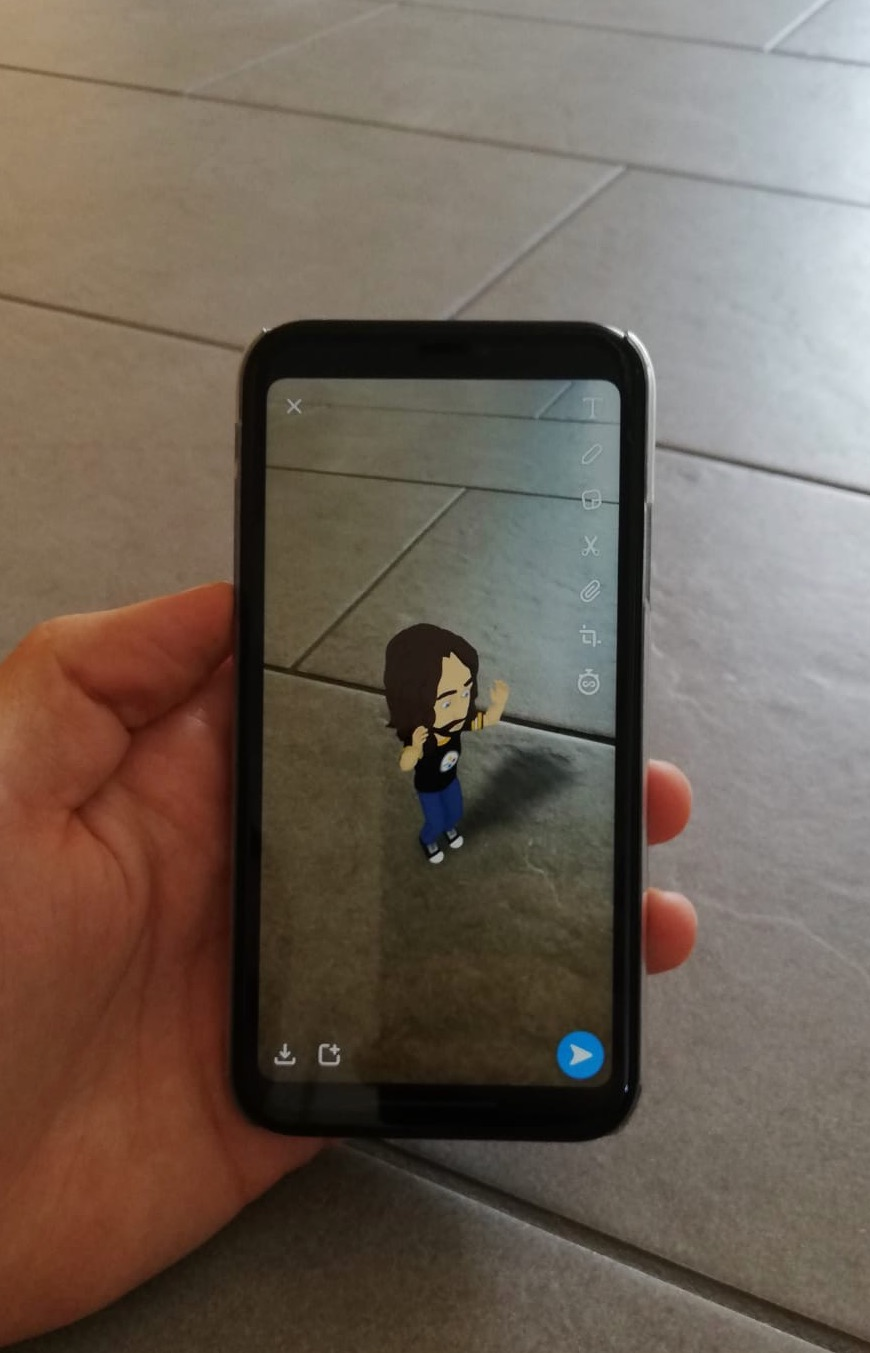
\includegraphics[width=6cm,height=6cm,keepaspectratio]{2Grundlagen/Bilder/snapchatAR.jpeg}
    \caption{Mobile-AR in Snapchat}
    \label{pic:snapchatAR}
\end{figure}
\pagebreak
\subsection*{Smart-Brillen AR}
\label{sec:smart-glasses}
Unter Smart- oder Datenbrillen und Smart Glasses wird ein Konstrukt verstanden, das eine Brille mit einem tragbaren Minicomputer verwirklicht. 
Dabei werden Informationen über kleinste Monitore oder Prismen ausgegeben und dem Nutzer zusätzlich in das Sichtfeld projiziert. Im Gegensatz
zur mobilen \acs{AR} hat der Nutzer kein Gerät in der Hand und ist somit in seiner Bewegung weniger eingeschränkt und flexibler. 
\\ 
\linebreak
Die Technologie der Smart-Brillen ist ein ähnliches Konzept zu der \acs{VR}-Brille, allerdings befindet sich die Smart-Brille für den 
öffentlichen Gebrauch noch in der Entwicklungsphase, da nur bedingte Funktionen möglich sind und die Kosten für den Normalverbraucher nur 
bedingt tragbar erscheinen. Mit der überarbeiteten Version der \textit{HoloLens 2} von Microsoft ist eine deutlich komfortablere und für 
den alltäglichen Gebrauch geeigneteren Ausführung entwickelt worden, die im Vergleich zum Vorgängermodell deutlich praktischer, leichter und handlicher ist. 
Das Design der Datenbrille ist von einer normalen Brille noch weit entfernt, ermöglicht mittlerweile aber das 
uneingeschränkte Sehen und Wahrnehmen der Umgebung. Die Bedienung des Geräts basiert auf schon vorhandenen Möglichkeiten die bereits in anderen 
Geräten Anwendung finden. Darunter gibt es am Gerät angebrachte Touchsensoren, Handbewegungen und -gesten und Eye-Tracking. 
\begin{figure}[hbt!]
    \centering
    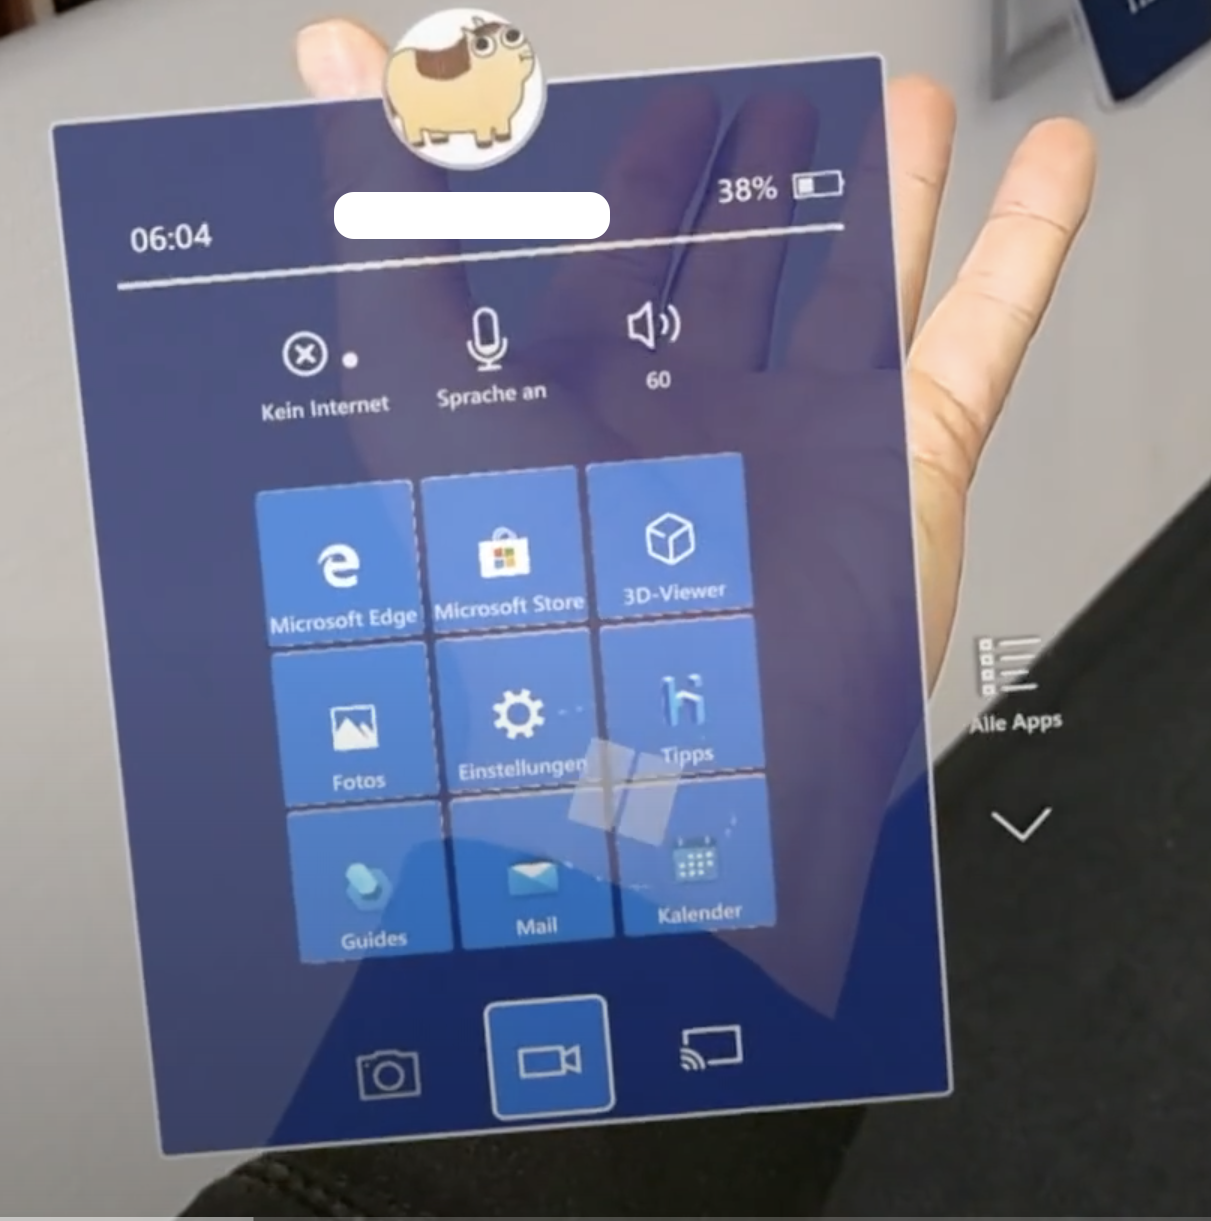
\includegraphics[width=10cm,height=7.5cm,keepaspectratio]{2Grundlagen/Bilder/smartglassAW.png}
    \caption{Test der HoloLens 2}
    \label{pic:testholo}
\end{figure}
\\ 
\linebreak %komfortables und
Speziell im industriellen Bezug bieten die neuentwickelten Brillen ein akzeptables Gewicht, sodass diese ohne große 
Probleme dauerhaft tragbar sind und den Mitarbeiter bei seiner Arbeit nicht übermäßig einschränken.
\\ 
\linebreak
Die Programmierung solcher \acs{AR}-Brillen laufen häufig über eigene \acs{SDK}s und plattformunabhängige Laufzeit- und 
Entwicklungsumgebungen, z.B. Unity oder Unreal Engine. Diese gelten als führende Produkte im Bereich der 3D-Echtzeitdarstellung.
Ein marktführendes Produkt ist unter anderem die Microsoft HoloLens 2, die der folgenden Abbildung zu entnehmen ist. 
\begin{figure}[hbt!]
    \centering
    \subfigure[Google Glass 2]{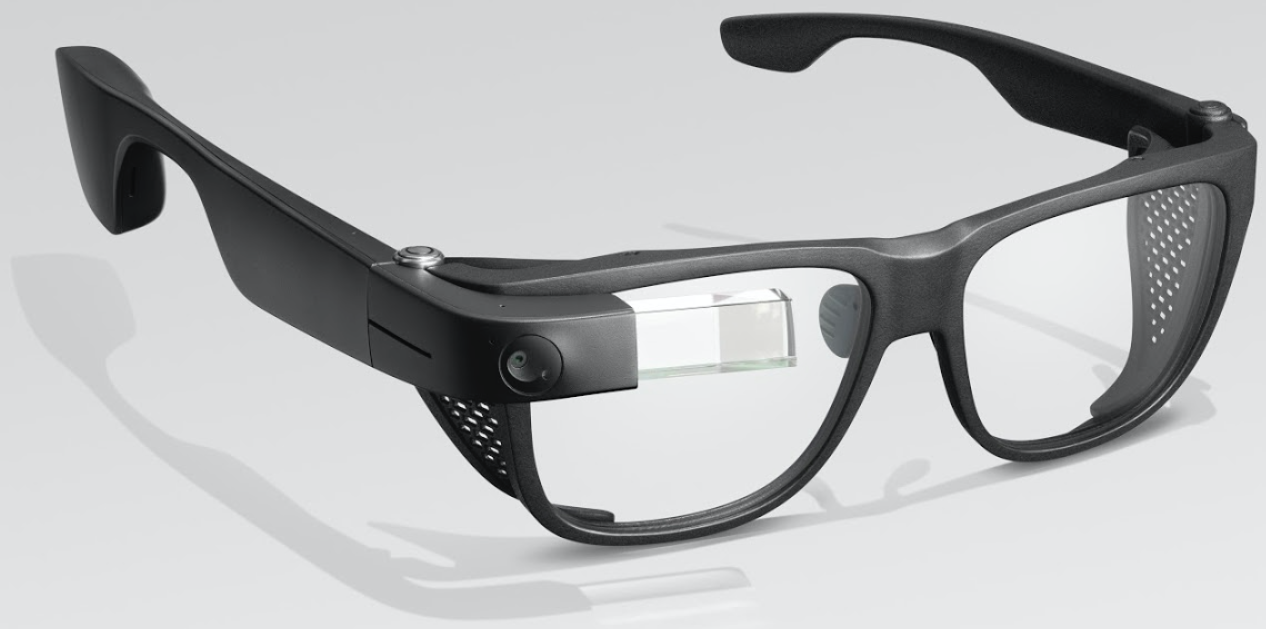
\includegraphics[width=7.5cm,height=5cm,keepaspectratio]{2Grundlagen/Bilder/googleglass.png}}
    \subfigure[HoloLens 2]{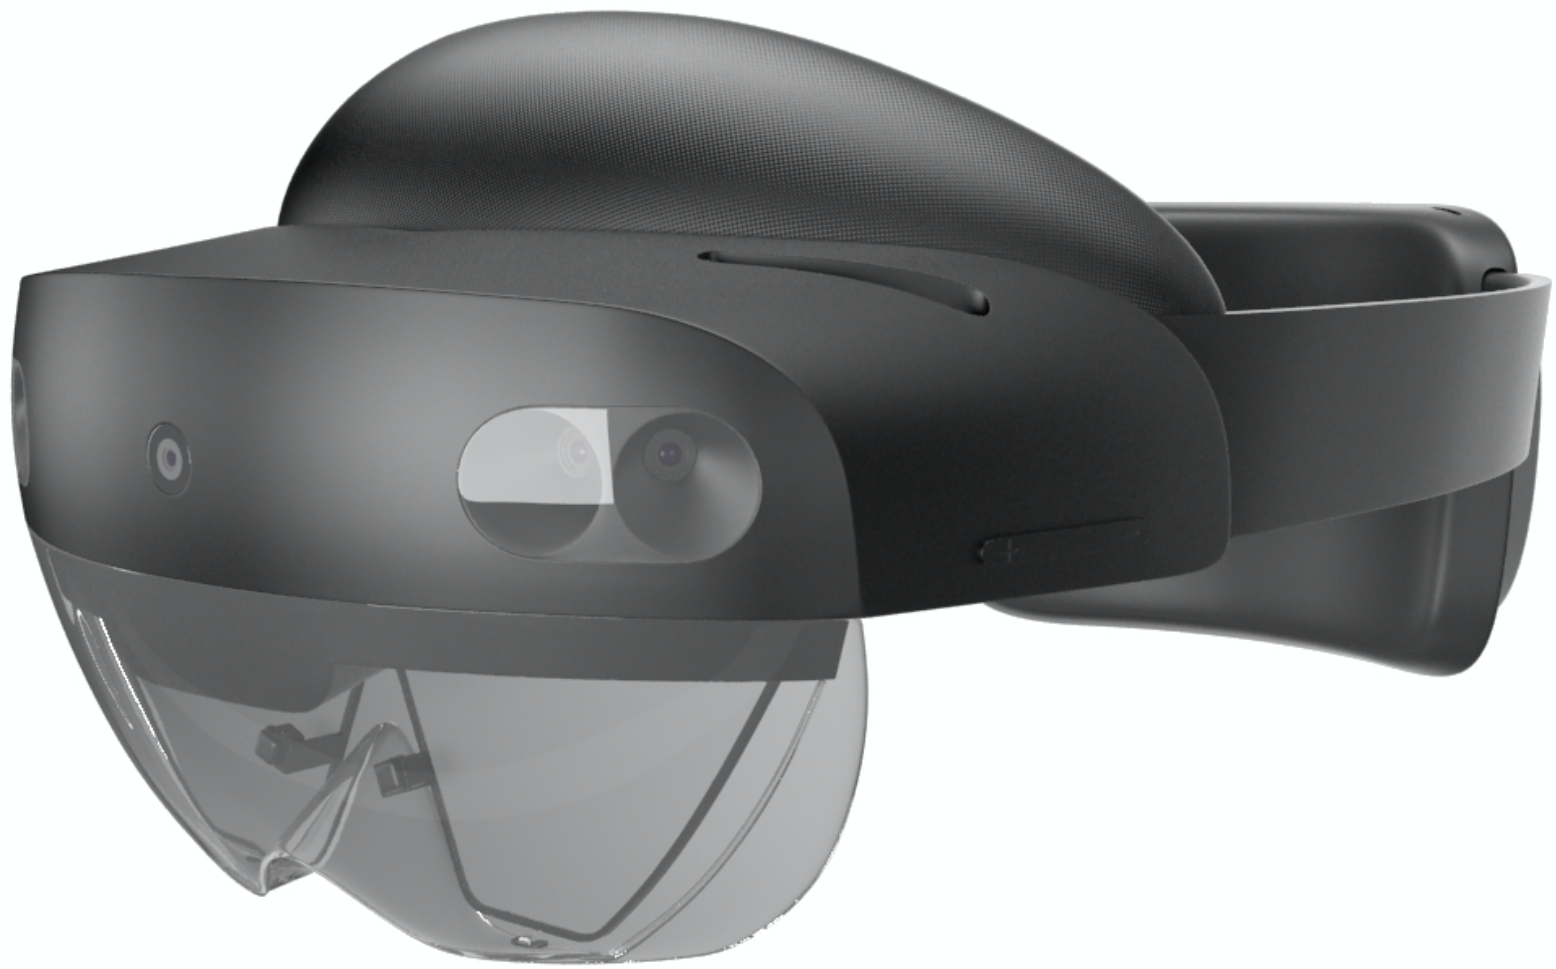
\includegraphics[width=7.5cm,height=5cm,keepaspectratio]{2Grundlagen/Bilder/hololensside.png}}
    \caption{Datenbrillen (\acs{HMD})}
    \label{pic:datenbrillen}
\end{figure}
\\ 
\linebreak
Eine große Herausforderung der \acl{AR} ist die Bestimmung der Position, in der Daten und Objekte projiziert werden. Auf die 
Ansätze, diese Herausforderung zu bewältigen, wird in folgendem Abschnitt \ref{sec:posi} eingegangen.
\subsection{Positionsbestimmung}
\label{sec:posi}
Um ein digitales Objekt als Overlay dem Kamera-Live-Bild hinzuzufügen, werden genauestens definierte Positionen benötigt. Diese Positionen 
können durch unterschiedliche Ansätze ermittelt werden. Je nach Anwendungsfall, z.B. als Navigation, Routenplaner oder Google Maps 
\textit{„Live View“} \cite{googleliveview.2019a}, reicht eine etwas ungenauere Positionsbestimmung per \acs{GPS}, da in Relation zur 
realen Welt eine Abweichung um Zentimeter oder wenige Meter nicht von Belang ist. Bei Positionsbestimmungen auf kleinstem Raum ist eine 
genaue Lokalisierung wichtig und basiert auf einem deutlich präziseren Ansatz. 
\\ 
Welche oben genannten Ansätze es gibt und welche Unterschiede zu beachten sind, wird in Folgendem näher erläutert. 
\subsubsection*{Marker-basierte Positionsbestimmung}
Speziell bei der Marker-basierten Positionsbestimmung gibt es verschiedene Möglichkeiten den Marker zu gestalten. Es können 
Binär- oder QR-Codes als Markierung verwendet werden, ein Beispiel eines solchen Codes ist der Abbildung \ref{pic:markerARpos} zu entnehmen. 
Diese Codes sind meistens quadratisch und haben ein eindeutiges Zeichen in der Mitte. Um die Rechenzeit gering zu halten gibt es einfache Muster, 
wie die Abbildung \ref{pic:markerARpos} zeigt.
\begin{figure}[hbt!]
    \centering
    
\includegraphics[width=5cm,height=5cm,keepaspectratio]{2Grundlagen/Bilder/bildmarkerAR.png}
    \caption{Marker-basierte Augmented Reality Positionsbestimmung}
    \label{pic:markerARpos}
\end{figure}
\pagebreak
\\ 
\linebreak
Neben der einfachen Markierungserkennung gibt es eine weiterentwickelte Möglichkeit der Bild- sowie der Objekterkennung. Diese sind Ansätze 
die grundlegend auf dem Ausgangspunkt des Binär-Code-Verfahrens aufbauen. Eine detailliertere Erläuterung der soeben genannten 
Erkennungsmöglichkeiten findet im Rahmen dieser Arbeit nicht statt, allerdings wird allgemein kurz auf die Funktionsweise einer 
Marker-basierten Positionsbestimmung eingegangen.
\\ 
Durch ein Kamerabild wird nach einem vordefinierten Marker, bzw. nach einer festgelegten Markierung gesucht. Ist diese mit der Kamera erfasst, 
wird die Markierung durch Bildverarbeitungsalgorithmen und bestimmter Filterung eindeutig identifiziert. Mit den gewonnen Informationen und 
der Übereinstimmung des angegebenen Codes wird die Position, sowie die Orientierung des Markers berechnet. Mit den Angaben der Lage und 
Orientierung wird auf der Markierung das anzuzeigende digitale Objekt generiert und als Overlay über dem Kamerabild angezeigt. Die Markierung 
dient sozusagen als Grundlage um den digitalen Gegenstand überhaupt anzeigen zu können.
\\ 
Da der Marker immer im Blickfeld der Kamera sein muss, um das virtuelle Objekt anzuzeigen, bringt diese Art der Positionsbestimmung eine 
enorme Einschränkung mit sich, die in diesem Bezug unumgänglich ist. 
\\ 
\linebreak
Ein weiterer Ansatz der Positionsbestimmung ist als Überbegriff das Gegenstück zur oben aufgeführten Lokalisierung von Markern, die 
sogenannte Marker-unabhängige Positionsbestimmung, welche ebenso verschiedene Ausführungen vorweist. 
\subsubsection*{\acs{GPS}-basierte Positionsbestimmung}
Die Methode des \acs{GPS}-basierten Positionsbestimmungsverfahren verwendet hauptsächlich die Koordinaten der realen Welt. In Zusammenarbeit 
mit zusätzlichen im Anwendungsgerät verbauten internen Sensoren, bspw. Positions-, Geschwindigkeits- und Beschleunigungssensoren und Teile des 
\ac{INS}, z.B. dem Gyroskop, kann diese Art der Positionsbestimmung optimal Anwendung finden. Allerdings werden dabei deutlich mehr Komponenten
benötigt und ist deutlich komplexer umzusetzen, als ein markerbasiertes System. 
\\ 
Bei einem Anwendungsfall von \acs{GPS}-basierter Positionsbestimmung geht es meist um Routenplaner, Navigation oder Szenarien die sich 
auf offenen Flächen abspielen, da im Gegensatz zu Marker-basierten Anwendungen das Größenverhältnis deutliche Unterschiede vorweist. 
Der Benutzer ist nicht auf einen bestimmten Bezirk beschränkt und ist nicht auf die millimetergenauer Darstellung angewiesen.
\\ 
\linebreak
Eine Alternative zu \acs{GPS} ist die Anwendung des \acs{SLAM}-Verfahrens. Dabei wird eine virtuelle Karte, bzw. ein geometrischen Modell der 
Umgebung erstellt. Wichtige Grundlagen zum Erzeugen eines solchen Modells sind eigenständig gefundene Landmarken die gleichzeitig 
lokalisiert werden. Darauf folgt ein Vergleich der Pose, der Position des Geräts und der geschätzten Karteninformationen aus dem Scan der 
Umgebung. 
Damit sind im erweiterten Sinne Marker geschaffen, die Anhaltspunkte für \acl{AR}-Interaktionen schaffen.
\\ 
In Kapitel \ref{chap:SLAM} wird die Thematik des \acs{SLAM}-Verfahrens erläutert. 

\subsection{Augmented Reality in der Industrie}
\label{sec:ARIndustrie}
Das weit gefächerte Portfolio der \acl{AR} umfasst viele Anwendungsbereiche und Fachgebiete. Selbst dem übergeordneten Bereich der Industrie 
gibt es viele verschiedene Einsatzgebiete. Aus den vielen Möglichkeiten der Anwendung haben sich über die Jahre der Entwicklung der Technologie 
einige Gebiete in der Industrie herauskristallisiert, die besonders großen Nutzen davon haben. \cite{einsatzgebietear.2017a} In den Bereichen 
Instandhaltung und Wartung, Betrieb und Training ist \acl{AR} auf bestem Wege, fester Bestandteil des Alltags zu werden. Bei dieser Betrachtung 
ist es sinnvoll, sich auf die damit einhergehenden Lösungen, die Reduktion der Kosten und dem Zeitaufwand, sowie die Verbesserung 
der Sicherheit, zu fokussieren. \cite{studieptc.2020j} 
\\ 
\linebreak
Bei einer Wartung oder Reparatur einer Maschine sind notwendige Informationen direkt greifbar und werden Schritt für Schritt angezeigt, sodass 
in bestimmten Situationen selbst ein Leihe die Anweisungen befolgen könnte. So werden zusätzliche Recherchearbeiten oder Unklarheiten über 
Vorgänge aus dem Weg geräumt. Ein Mitarbeiter kann so mit einem Tablet oder einer Smart-Glas Anweisungen visuell auf die realen Maschinen 
projizieren und Arbeitsschritte im Sichtfeld anzeigen lassen. Ebenso geht dieser Vorgang auch bei der Produktion von Bauteilen o.ä., indem 
eine \acs{AR}-Anwendung Anweisungen und Prozessschritte, z.B. auf das Werkstück oder Produkt, projiziert.
\\ 
Die Inbetriebnahme oder Bedienung einer komplexen Anlage oder Maschine ist nach herkömmlichen Standard enorm zeitintensiv und dadurch können
zusätzlich viele Fragen aufkommen, die meist den Prozess noch länger gestalten als vorgesehen. \acs{AR}-Anwendungen können 
Bedienungsanleitung oder -hilfen digitalisiert, indem Informationen, Inhalte oder Bedienelemente durch \acl{AR} auf der Anlage platziert werden. 
\\ 
In Fortbildungen, Schulungen oder Einarbeitungen in neue Geräte kann \acs{AR} durchaus von großem Vorteil sein. Mit wenig Aufwand, einem 
effektiveren Training können Schulungen interaktiver und vor allem sicherer abgehalten werden. Durch die Visualisierung der Trainings- und 
Schulungsinhalten verbessert sich der Lernprozess und damit wird auch die Nutzung der Maschinen verständlicher. \cite{einsatzgebietear.2017a}
% \section{SLAM - Simultanious Localization And Mapping}
\label{chap:SLAM}
Als Simultaneous Localization and Mapping, auch \acs{SLAM}-Problem genannt, bezeichnet man die Aufgabe, die Trajektorie\footnote{Lösungskurve oder Bewegungspfad eines Objekts} 
samt Orientierungsinformation einer sich bewegenden Plattform, z.B. ein Smartphone, Tablet oder jegliche Art von Roboter, aus 
Beobachtungen zu schätzen und gleichzeitig aus den gewonnenen Informationen eine Karte der Umgebung zu erstellen.
Diese Aufgabe ist für den weiteren Prozess bedeutend. Zum einen sollen die generierten Karten sehr präzise sein, um einen hohen 
Wert für den Nutzer oder für spezielle auf der Karte aufbauende Anwendungen darzustellen. Zum anderen benötigen autonome Roboter, 
beispielsweise Saug- oder Mähroboter, ein solch erzeugtes geometrisches Modell der Umgebung, um zielgerichtet selbstständig navigieren zu 
können. %\cite{slamdefi.2016a} 
\begin{quote}
    Das Simultaneous Localization and Mapping oder kurz SLAM Problem behandelt das gleichzeitige Schätzen der Position und Ausrichtung einer 
    mobilen Plattform im Raum anhand der sich an Bord befindlichen Sensoren sowie den Aufbau eines Modells der Umgebung. Dieses Problem ist 
    von großer praktischer Relevanz und ist Kernbestandteil der meisten mobilen Sensorsysteme. \cite{slamdefi.2016a}
\end{quote}
1986 wurden auf der \textit{IEEE Robotics and Automation Conference} erste mathematische Definitionen vorgenommen, die mittels statischer 
Theorien ermittelt und mit ersten Studien belegt wurden. Einige Jahre später, im Jahr 1995, wurde das \acs{SLAM} Problem erstmals auf dem 
internationalen Symposium für Robotikforschung (\textit{ISRR'95}) vorgestellt. Die Forschungen hielten an, bis auf der \textit{ISRR'99} 
die erste \acs{SLAM} Sitzung stattfand. 

\subsection{Definition des Problems}
Angenommen ein Roboter startet in einer Position, auch Pose genannt, und einer Konfiguration \textit{p0} und bewegt sich durch eine ihm 
unbekannte Umgebung, stellen die nicht vorhandenen Kenntnisse seiner Position und der damit verbundenen Orientierung das Hauptproblem dar. 
Die Einstellung beinhaltet Position und Ausrichtung des Roboters. Je nach Bewegung in Raum oder Ebene ist die Pose meist als 3- oder 
6-dimensionaler Vektor abgebildet. Die Bewegung des 
Roboters wird durch bekannte Kontrollkommandos \textit{u} angewiesen, allerdings mit einer gewissen Unsicherheit versehen. Dabei wird 
zwischen den Zeitpunkten \textit{t-1} und \textit{t} die Bewegung des Roboters mit \textit{ut} beschrieben und somit auch die 
unterschiedlichen Posen \textit{pt-1} nach \textit{pt}. Die Umgebung wird parallel dazu über diverse Sensoren, z.B. interne Sensoren, bspw. 
Geschwindigkeits- oder Positionssensoren, und externer Sensoren, unter anderem Abstands- oder taktile Sensoren. Neben der Protokollierung der 
Position, bei der es zu Störungen oder Berechnungsfehlern kommen kann, gibt es Beobachtungen durch Sensoren die verrauscht, bzw. fehlerhaft 
sind und durch \textit{zt} angegeben werden.
\\ 
\linebreak
Mit diesen vorhandenen Werten ist die Schätzung der Trajektorie \textit{p0:T=[p0,p1,...,pT]T} des Roboters von Beginn der 
Fortbewegung bis zum Zeitpunkt \textit{T} das Ziel. Gleichzeitig zur Berechnung der Trajektorie wird eine Karte \textit{m} des Umfelds geschätzt, 
deren Darstellung den Anforderungen entsprechend angepasst werden kann. Mit den Anforderungen sind verschiedene Repräsentationen der Karten 
gemeint, darunter beispielsweise eine Veranschaulichung von Punktansammlungen an Gegenständen, gerenderte Oberflächenmodelle oder 
2D-Rasterkarten und verstärkt visualisierte 3D-Voxelkarten\footnote{(Zusammensetzung aus dem englischen volume \textit{vox} und elements 
\textit{el}), bez. einen Gitterpunkt in einem dreidimensionalen Gitter.}. Basierend auf den Sensormessintervallen \textit{z1:T} und den dabei
stattfindenden Kontrollkommandos \textit{u1:T} wird die Karte des Umfeldes und alle Positionen bestimmt. Die Wahrscheinlichkeitsverteilung 
\textit{p(p0:T,m|z1:T,u1:T)} wird durch die geschätzten Werte \textit{p0:T} und \textit{m} berechnet. 
\\ 
\linebreak
Die Berechnung der Wahrscheinlichkeitsverteilung ist auch unter dem Namen \textit{Offline-\acs{SLAM}} bekannt. In der Praxis ist allerdings 
die Schätzung der Position \textit{xt} und der Karte der Umgebung durch \textit{p(pt,m|z1:t,u1:t)} interessanter, da Roboter Entscheidungen 
basierend auf aktuellen Informationen, z.B. der Posenschätzung und dem Umgebungsmodell, treffen sollen. Die Variante der Echtzeitschätzung 
ist auch als \textit{Online-SLAM} bekannt. \cite{slamdefi.2016a}

\subsection{Localization}
Damit das Endgerät, Smartphone oder der Roboter seine Position in Erfahrung bringen und schätzen kann, werden Informationen und Möglichkeiten 
benötigt, die Bewegung in irgendeiner Form zu messen. Da das Nutzergerät eine eigene virtuelle Karte, unabhängig von der \acs{GPS}-basierten 
Position, generiert, ist das \textit{Tracking} über die Weltkoordinaten nicht Bestandteil des eigentlichen Verfahrens. Für die Erfassung der 
internen Systemzustände gibt es sogenannte interne Sensoren die in dem Roboter zur Verfügung stehen. Bestandteile dieser internen 
Sensorik sind unter anderem Positions-, Geschwindigkeits-, Beschleunigungssensoren und das \acl{INS}. Für die Positions- und 
Geschwindigkeitserkennung gibt es z.B. einen optischen Codierer, welcher durch Lichtimpulse die Geschwindigkeit als auch die zurückgelegte 
Strecke schätzen kann. Das \acs{INS} besteht aus Lagesensoren und einem Kreiselkompass (Gyroskop). Diese sind essentiell für die Bestimmung 
der Orientierung und Neigung des Geräts. Ausgehend von der Erdkugel beziehen sich diese Sensoren auf das gegebene inertiale Koordinatensystem.
Mittels \textit{Odometrie} können die von den Sensoren bereitgestellten Informationen über Position und Orientierung berechnet werden. Radgetriebene 
Systeme führen die Berechnung durch, da diese basierend auf dem Durchmesser des Rades ermittelt wird. In Kombination mit \textit{Koppelnavigation}\footnote{Engl. dead reckoning, ist die laufende Positionsbestimmung eines bewegten Objekts infolge der Bewegungsrichtung und Geschwindigkeit \cite{koppelnavigation.2019j}}
gilt dieses Verfahren für Roboter, bzw. Fahrzeuge auf Land, als Grundlage der Navigation. Durch die theoretische Berechnung werden 
Fehlerbetrachtungen, z.B. Verschleiß, Schlupf oder Unrundheit von Rädern, vernachlässigt und ist somit nicht als alleiniges Verfahren einzusetzen. 
\begin{align}
    \Delta U = \frac{\pi D}{\textit{n}C}N
\end{align}
Mit \textit{D} als Raddurchmesser, \textit{n} als Getriebeübersetzung, \textit{C} als Enkoderauflösung und \textit{N} als Anzahl der 
Enkoderimpulse wird die Positions- und Orientierung berechnet. 
\\ 
Smartphones berechnen die Fortbewegung über gegebene Sensoren, darunter Beschleunigungs- und Neigungssensoren und Gyroskop. Dieses Zusammenspiel an 
Sensoren ermöglicht die Wahrnehmung der Positionsveränderung und kann somit diese bestimmen.
\subsection{Mapping}
Um neben der Berechnung der Position durch die interne Sensorik die Umgebung registrieren und schätzen zu können, gibt es externe Sensoren, 
die sich mit der Erfassung der Umwelt beschäftigen. Auch hier gibt es viele Arten von Sensoren, mit denen es ermöglicht wird, die Umgebung 
wahrzunehmen. Darunter sind taktile Sensoren, Näherungs-, Abstands-, Positionssensoren und visuelle Sensoren. Hinsichtlich Abstandssensoren, die 
Messungen zwischen Gegenstand und Sensor durchführen, gibt es im Allgemeinen erhebliche Vorteile gegenüber den Näherungssensoren. Unter Anderem 
besitzen sie zum Beispiel eine größere Reichweite und ein größeres Blickfeld als Näherungssensoren. Somit können sie die Entfernung zu Gegenstände 
genauer ermitteln und geometrische Umweltinformationen besser erfassen. Für die Messung des Abstandes eignet sich die \ac{TOF}-Kamera, die 
mit dem Laufzeitverfahren Distanzen messen und berechnen kann. 
\\ 
Das Laufzeitverfahren funktioniert wie folgt:
\begin{align}
    \textit{d} = \frac{1}{2}\textit{ct}
\end{align}
Abstand zwischen der Zielfläche und dem Sensor \textit{d} ist das Produkt aus der Signalgeschwindigkeit \textit{c} und der messbaren Laufzeit 
\textit{t}. Beispiele für solche \acs{TOF}-Kameras und deren Repräsentation sind folgender Abbildung (\ref{pic:tofCam}) zu entnehmen.
\begin{figure}[hbt!]
    \centering
    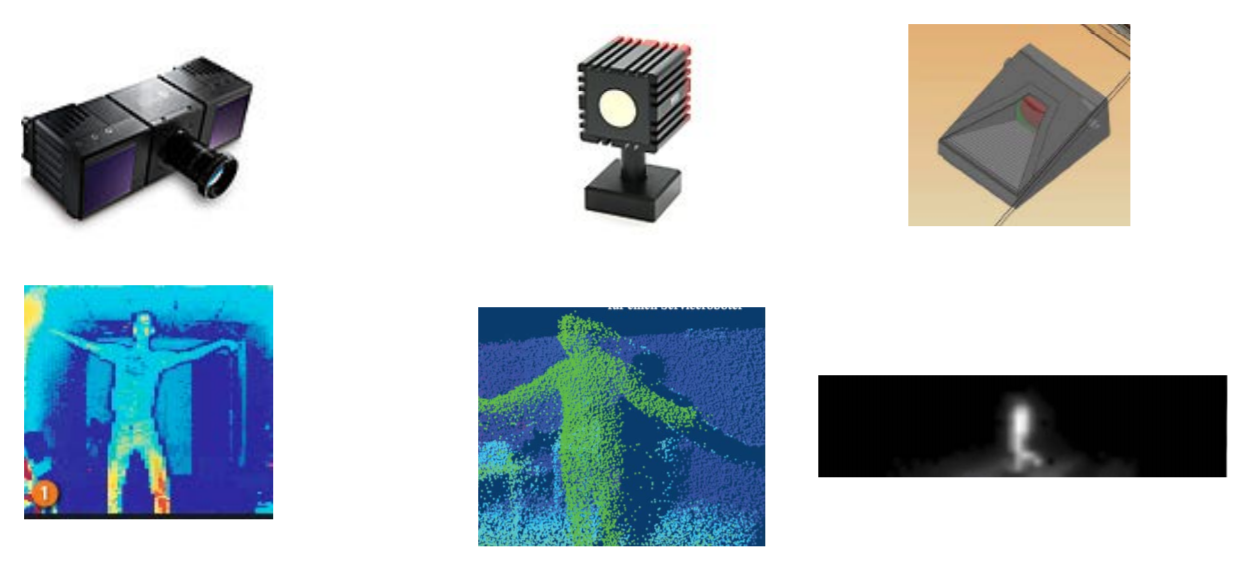
\includegraphics[width=13cm,height=13cm,keepaspectratio]{2Grundlagen/Bilder/tof_kamera.png}
    \caption{Time-of-Flight Kamera und deren Repräsentation \cite{robotik.2020m}}
    \label{pic:tofCam}
\end{figure}
\\ 
Auf der linken Seite ist eine PMD-Kamera zu sehen, gefolgt von einer SwissRanger-Kamera und auf der rechten Seite eine IFM-Kamera.

\subsection{Verfahren zur Lösung des SLAM Problems}
Das Lösen des \acs{SLAM} Problems wird in der Praxis mit den folgenden Verfahren, die sich bei der Anwendung bewährt haben, durchgeführt. In den 
folgenden Abschnitten werden zwei dieser Verfahren erläutert, sodass ein Grundverständnis der Funktionsweisen der Verfahren entsteht. 
Als Erstes erfolgt eine nähere Erläuterung des graph-basierten \acs{SLAM} Verfahren, gefolgt von der Lösung des Problems mit einem rekursiven 
Ansatz, dem erweiterten Kalman Filter (\acs{EKF}).

\subsection*{Graph-basiertes SLAM Verfahren}
Grundlegend wird bei dem Algorithmus des graph-basierten Verfahrens, während der Bewegungsaufzeichnung des Roboters, ein Graph modelliert, 
dessen Positionen zu verschiedenen Zeitpunkten durch Knoten dargestellt werden. Alle nebeneinander liegenden Positionen, bzw. Punkte, die 
lediglich minimale Unterschiede in der Umgebung aufweisen, werden zu einem Punkt gebündelt. Diese korrespondierenden Positionen, bzw. 
Knoten im Graphen werden über eine Kante verknüpft. Gebunden an die Bewegung des Roboters werden die Kanten modelliert. Der folgende Graph 
(\ref{pic:GraphSLAM}) veranschaulicht ein solches Modell.
\begin{figure}[hbt!]
    \centering
    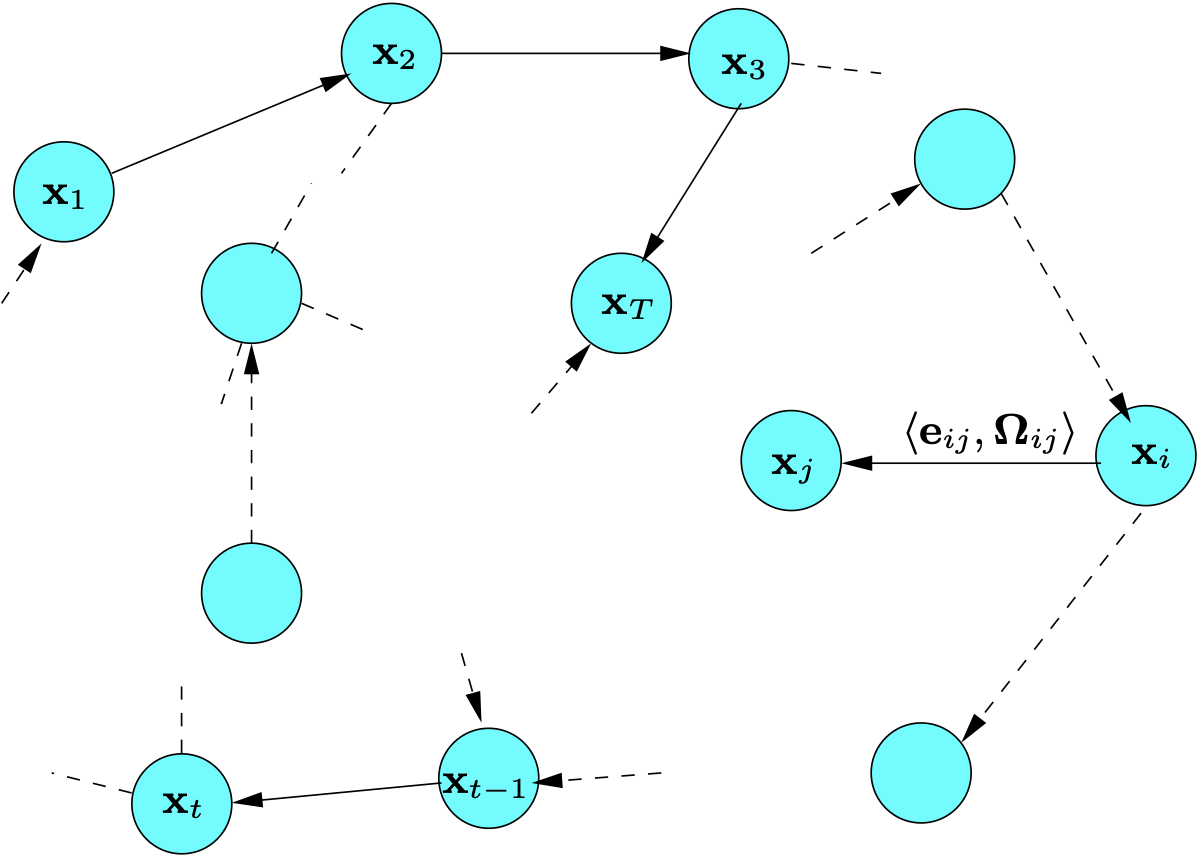
\includegraphics[width=10cm,height=10cm,keepaspectratio]{2Grundlagen/Bilder/graph_SLAM.png}
    \caption{Graphische Darstellung des SLAM Verfahrens \cite{graphSLAM.2010}}
    \label{pic:GraphSLAM}
\end{figure}
\\ 
Der Abbildung ist zu entnehmen, dass der Graph auch Kanten darstellt, die nicht den folgernden Knoten ansprechen, sondern eine 
Position vertreten, die in ihrer Beobachtung auf korrespondierende Knoten zurückgeht. Durch wiederholte Scans können genauere Merkmale und 
Bedingungen festgelegt werden, um die daraus resultierenden Positionen besser differenzieren zu können. Bei Verwendung von Kameras können 
genauer identifizierten Merkmale die geschätzten relativen Orientierungen sein, die durch eine zusätzliche Funktion berechnet werden 
können. Bei der Nutzung eines Lasersensors wird meist der \ac{ICP} Algorithmus angewendet, um die Veränderungen zwischen den Aufnahmepositionen 
wahrzunehmen. \acs{ICP} ist ein iteratives, ständig wiederholendes Verfahren, das die korrespondierenden Punkte schätzt und solange transformiert, bis diese unter 
einem gewissen Schwellwert liegen. Korrespondierende Punkte sind die, die den kleinsten Abstand zueinander haben (Closest Point). \cite{robotik2.2020m}
\\ 
Der inkrementelle Ansatz des graph-basierten \acs{SLAM} Verfahrens ist ursprünglich ein \textit{offline-Verfahren}, welches über die Jahre 
schrittweise zu einem \textit{online-Verfahren} führte. Durch diese ständige Beobachtung und Neuberechnung der aktuellen Position zu jedem 
Zeitpunkt wurde die Bedeutung der inkrementellen Verfahren gesteigert. %Dieser Ansatz ist besonders für monokulare Kameras ratsam und sinnvoll.

\subsection*{Rekursives Schätzproblem}
Der erweiterte Kalman-Filter (\acs{EKF}) ist eine wahrscheinlichkeitsbasierte rekursive Schätzung der Position des Objekts und der Position der 
Landmarken unter Nutzung linearer Bewegungsmuster basierend auf dem Bayes-Filter. Der Bayes-Filter-Algorithmus ist das generelle Verfahren der 
rekursiven Zustandsschätzung und wird über den Satz von Bayes\footnote{Mathematischer Satz der Wahrscheinlichkeitstheorie. Daruch wird die Berechnung einer bedingten Wahrscheinlichkeit beschrieben} 
hergeleitet. 
\\
Unter der Voraussetzung einer Normalverteilung und eines linearen Bewegungsmodells, worauf der Kalman-Filter setzt, kann diese durch das 
\acs{SLAM} Problem nicht erfüllt werden. An dieser Stelle wird der erweiterte Kalman-Filter eingesetzt, da dieser nicht-lineare 
Bewegungsmodelle, bzw. Funktionen mittels Taylorreihe approximiert. Somit kann eine Messung in etwas vorhergesagt werden. Diese Schätzung 
dient somit als Grundlage zur eigentlichen Messung. Nach der Berechnung wird der Zustand aktualisiert und ausgegeben. Mit diesem Ergebnis 
werden die darauffolgenden Punkte rekursiv berechnet, bis die Scan-Phase zu Ende ist.

\section{Quaternionen}
\label{chap:Quaternionen} %\cite{quaternionHamilton.2006} 
Quaternionen, lat. \textit{„Menge der Vier“}, wurden erstmals 1843 von Sir William Rowan Hamilton beschrieben. Sie bezeichnen einen 
Zahlenbereich, der die reellen Zahlen erweitert. Die mathematische Formel wird häufig zur Darstellung einer Drehung im dreidimensionalen Raum 
verwendet. Die Theorie der Quaternionen basiert auf der mathematischen Grundlage der komplexen Zahlen, die 1833 von Hamilton als Bildung 
einer Algebra galten und werden daher als hyperkomplexe Zahlen aufgefasst.
\\ 
\linebreak
Mit \textit{a,b,c,d $\in q$} werden Quaternionen wie folgt beschrieben:
\begin{align}
    \textit{q} = \textit{a} + \textit{b} \cdot \textit{i} + \textit{c} \cdot \textit{j} + \textit{d} \cdot \textit{k}
\end{align}
In oben genannter Formel ist die Variable \textit{a} der Realteil und (\textit{b,c,d})$^T$ der Imaginärteil \textit{u} der Gleichung. 
Auch geschrieben als \textit{q = (a, u)$^T$}, um die Teile differenzieren zu können. 
\\ 
Mit der sogenannten \textit{Brougham Bridge}-Formel ist es möglich Vektoren zu dividieren. 
\begin{subequations}
    \label{Quaternionen-Gleichung}
    \begin{align}
        \textit{i$^2$} = \textit{j$^2$} = \textit{k$^2$} = \textit{ijk} = \textit{-1} 
        \label{erstes Gleichungsgesetz} \\
        \textit{ij} = \textit{-ji} = \textit{k} 
        \label{zweites Gleichungsgesetz} \\
        \textit{jk} = \textit{-kj} = \textit{i} 
        \label{drittes Gleichungsgesetz} \\ 
        \textit{i$^2$} = \textit{j$^2$} = \textit{j}
    \end{align}
\end{subequations}
\subsection{Rotation}
%\subsection{Transformation}
Quaternionen dienen als Möglichkeit, Drehungen, bzw. Rotationen darzustellen, unter anderem wegen der reduzierten Anzahl an 
benötigten Parametern im Vergleich zur Berechnung von Rotationsmatrizen und deren Translation. Die Quaternionen bieten eine deutlich kompaktere 
Darstellung der Rechenwege. Somit können Rotationen intuitiver veranschaulicht werden, d.h. es sind direkte Angaben von Drehwinkel und 
-achse möglich. Die kompaktere Darbietung beinhaltet lediglich vier Werte im Vergleich zu den neun Werten der Berechnung der Rotationsmatrix
und die Rotation kann um eine bestimmte Achse ermittelt werden. Zudem ist eine sehr hohe numerische Stabilität gewährleistet. 
\\ 
Der Drehwinkel wird wie folgt berechnet:
\begin{align}
    %\textit{a} = $\cos z$ \to \textit{z} = \frac{t}{2} \to t = $\theta$  %\textit{z} = \textit{\frac{$\theta$}{2}} 
    %\\
    \textit{$\theta$} = \textit{2} \cdot \textit{$\arccos a$}
\end{align}
Der Realteil \textit{a} des Quaternions wird mittels Arkuskosinus berechnet, so erhält man die Drehung des Objekts. Die Drehachse lässt sich 
bestimmen, indem alle Werte des Imaginärteils (\textit{b,c,d})$^T$ mit \textit{u} addiert werden. Die Variable \textit{u} setzt sich wie 
folgt zusammen: 
\begin{align}
    \textit{u} = \textit{$\sin w$}, \to \textit{w} = \frac{t}{2}, \to \textit{t = $\theta$}
\end{align}
Mit diesen zwei Berechnungen werden Drehwinkel und Drehachse bestimmt und können für weitere Berechnungen verwendet werden.

\section{Technologien}
\label{chap:Technologien}
Dieser Abschnitt befasst sich mit den wichtigsten Programmier-Technologien, die in diesem Projekt eingesetzt werden. 
%Ein kurzer Überblick 
%über die Historie der Technologien, worum es dabei geht und welche Aufgaben sie umfassen. 
\\ 
Der Augenmerk liegt auf dem Framework \textit{Google ARCore}, da dieses Hauptbestandteil des Projekts ist. 
\subsection{Google ARCore}
\label{sec:arcore}
ARCore ist die von Google veröffentlichte Plattform zum Erstellen von \acl{AR} Erlebnissen, primär entwickelt für Android Phones. 
Das \ac{SDK} ist in den Programmiersprachen Java und Kotlin geschrieben. Mit bestimmten \acs{API}s ermöglicht \textit{ARCore} die Erfassung 
der Umgebung durch ein Tablet oder Smartphone, um so die Welt zu verstehen. Mitte des Jahres 2017 
wurde die \textit{Google ARCore API} zum ersten Mal den Entwicklern und der \acs{AR}-Community präsentiert. Im ersten Quartal 2018 wurde 
diese dann veröffentlicht und löste das Vorreiterprojekt \textit{„Project Tango“} ab. 
\\ 
\linebreak 
\textit{Project Tango} war ebenso eine Google-Plattform, mit dem Smartphones und Tablets ein \textit{„Raumgefühl“} erhalten. \cite{projecttango.2016j} 
Die Plattform kombinierte die Eingabe verschiedener Sensoren, z.B. radarähnliche Infrarotstrahler, einer Infrarotkamera und hochpräzisen 
Beschleunigungsmessern, Barometern und Gyroskopen, um schnell nutzbare Informationen der Umgebung zu generieren. Mit der Überarbeitung des 
Konzepts wurde das neue unabhängige Projekt \textit{ARCore} geschaffen und somit die Anzahl der Hardwarekomponenten reduziert, bspw. wird 
keine spezielle Infrarotkamera mehr benötigt. Die ARCore \acs{API} verwendet bei Anwendungen ausschließlich das Kamerabild des Smartphones und 
dessen Sensoren. 
\\ 
\linebreak 
Zum Integrieren von virtuellen Objekten in die reale Welt verwendet ARCore drei Schlüsselfunktionen unter Benutzung von Java und OpenGL, Unity 
und Unreal:
\begin{itemize}
    \item Motion tracking, dt. Bewegungsverfolgung, ermöglicht das Verstehen und Verfolgen der Position des Geräts relativ zur Realität.
    \item Environmental understanding, dt. Verständnis der Umgebung, erkennt die Position und Größe aller Arten von Oberflächen: horizontale, 
    vertikale und abgewinkelte Oberflächen, wie Wände, Böden, Tische oder Stühle.
    \item Light estimation, dt. Lichtschätzung, schätzt die durch das Smartphone gegebenen Lichtverhältnisse der Umgebung. \cite{arcorefundamentals.2018m}
\end{itemize}
% \subsubsection*{Motion tracking}
Für die Funktion der Bewegungsverfolgung verwendet ARCore das Verfahren von \acl{SLAM} (\acs{SLAM}) \ref{chap:SLAM}, um so zu verstehen wo 
sich das Smartphone in Relation zur realen Welt befindet. Zusätzlich erkennt ARCore visuell unterschiedliche Merkmale im aktuell aufgenommenen 
Kamerabild, sogenannte Merkmalspunkte \textit{„feature points“}. Anhand dieser Punkte wird die Änderung des Standortes berechnet. Durch Trägheitsmessungen 
der \ac{IMU}, dt. Inertiale Messeinheit des Geräts, kombiniert mit den visuellen Informationen des Kamerabildes wird die Position und 
Ausrichtung der Kamera in Relation zur Realität abgeschätzt. 
\begin{figure}[hbt!]
    \centering
    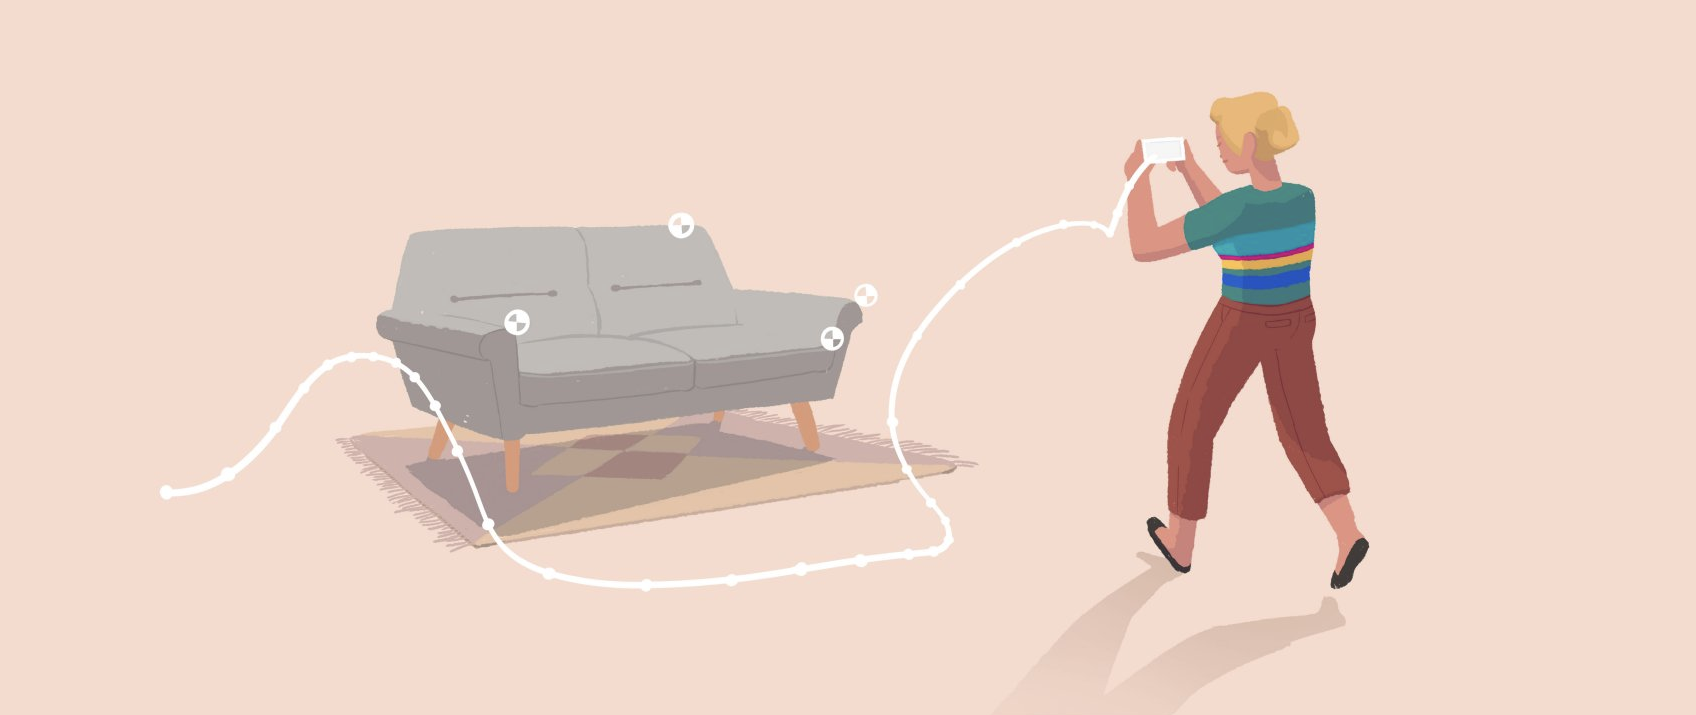
\includegraphics[width=15cm,height=5cm,keepaspectratio]{2Grundlagen/Bilder/motionTracking.png}
    \caption{Skizze zur Bewegungsverfolgung des Smartphones \cite{arcoreofficial.2020j}}
    \label{pic:motiontracking}
\end{figure}
\\ 
Die \acl{IMU} in Smart-Devices besitzt drei Beschleunigungssensoren, z.B. piezoelektrische Beschleunigungssensoren oder \ac{MEMS}, für die 
drei Raumachsen:
\begin{itemize}
    \item Die Abszissenachse (X-Achse), die horizontale (waagerechte) Koordinatenachse,
    \item Die Ordinatenachse (Y-Achse), die darauf vertikale (senkrechte) Koordinatenachse und
    \item Die Applikatenachse (Z-Achse), die auf beiden anderen Achsen senkrechte Achse \cite{koordinatennorm.1973m}
\end{itemize}
Ebenso besitzt die \acs{IMU} Drehratensensoren, z.B. ein Gyroskop zur Messung der Rotationsgeschwindigkeit, welche die Drehraten um 
diese Raumachsen messen. Durch die kontinuierliche Auslesung der Sensordaten, wird die Position des Geräts berechnet und in Form von 
drei Koordinaten ausgegeben. Ausgehend von dem Referenzkoordinatensystem wird die Position neu bestimmt. Die Abbildung \ref{pic:Positionsberechnung} 
veranschaulicht solch ein Beispiel.
\begin{figure}[hbt!]
    \centering
    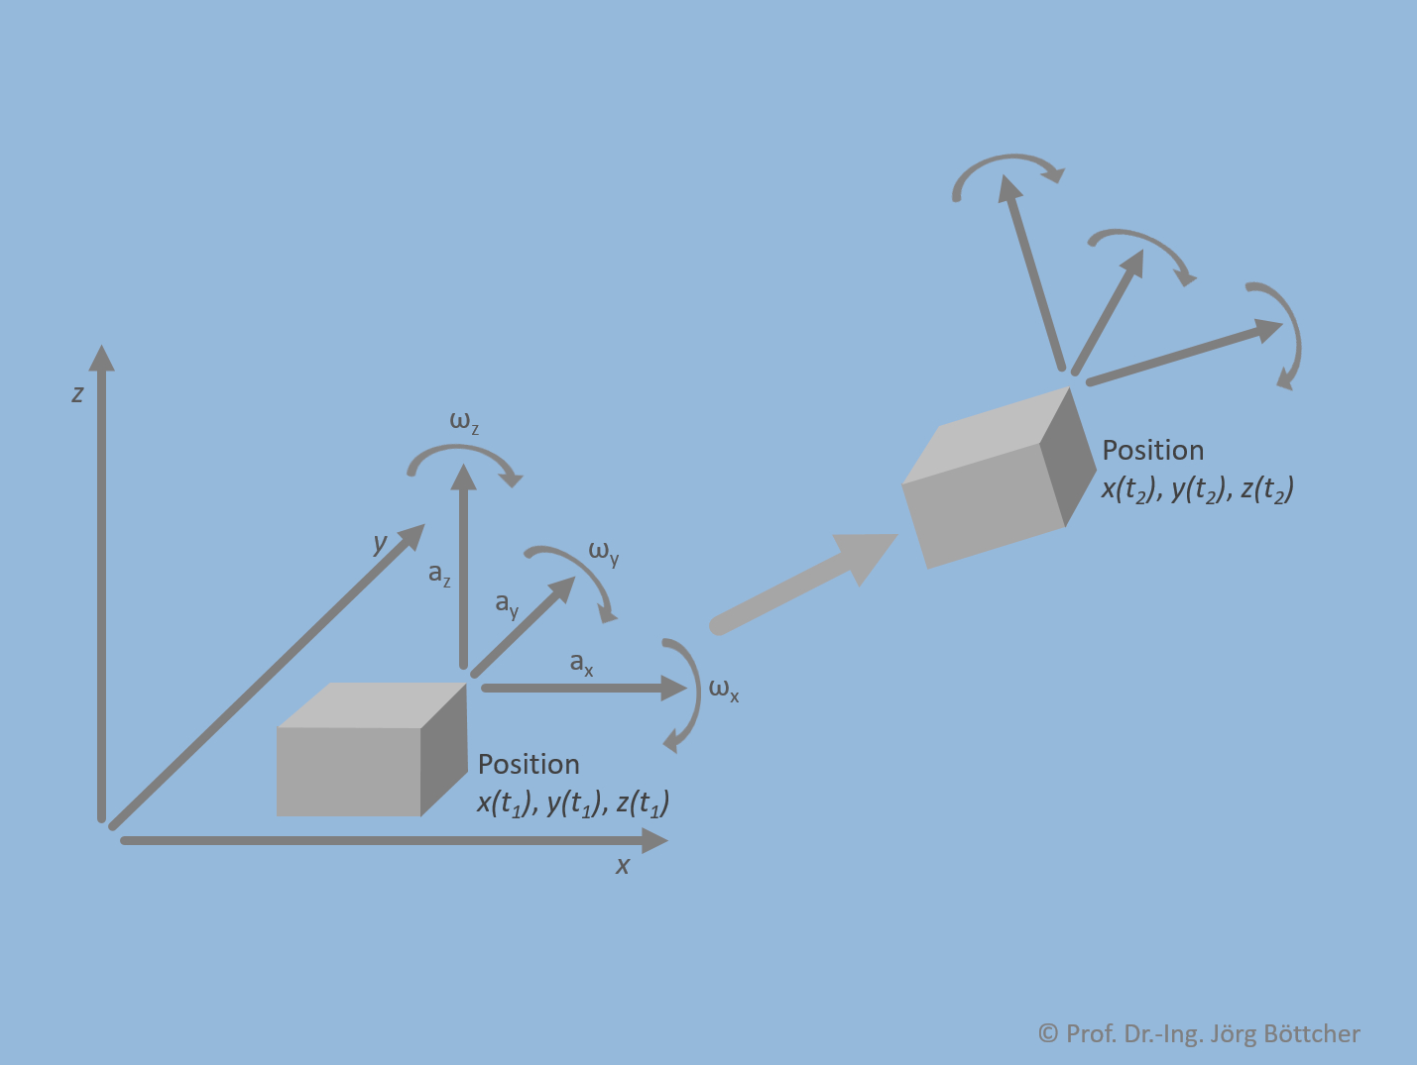
\includegraphics[width=9cm,height=9cm,keepaspectratio]{2Grundlagen/Bilder/imu-Bsp.png}
    \caption{Grundprinzip einer IMU \cite{imubild.2020j}}
    \label{pic:Positionsberechnung}
\end{figure}
\pagebreak
\subsubsection*{Environmental understanding}
Die zweite Schlüsselfunktion des Frameworks ist das Verständnis der Umgebung. Dieses wird erlangt, indem \textit{„feature points“}, Ebenen und 
Flächen beim scannen des Umfelds erkannt werden. Beim Entstehen mehrerer solcher \textit{feature points} erstellt ARCore ein Cluster aller 
naheliegenden Punkte. Dieses erzeugte Cluster repräsentiert eine horizontale oder vertikale Fläche. Mit diesen gewonnenen Informationen ist das 
Platzieren von virtuellen Objekten auf den erfassten Flächen möglich.
\begin{figure}[hbt!]
    \centering
    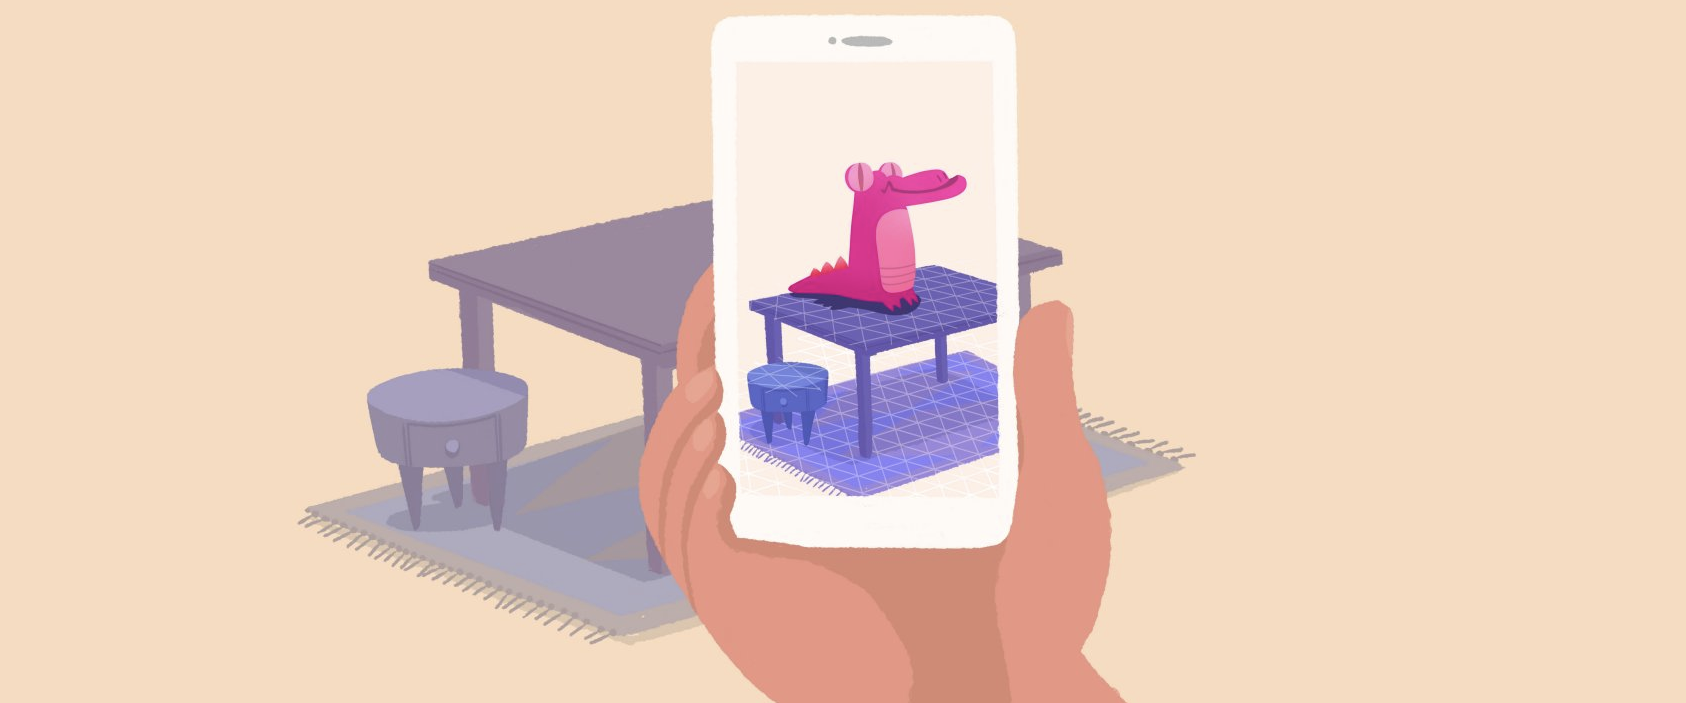
\includegraphics[width=15cm,height=5cm,keepaspectratio]{2Grundlagen/Bilder/environmentalUnderst.png}
    \caption{Skizze zum Umgebungsverständnis des Smartphones \cite{arcoreofficial.2020j}}
    \label{pic:environmentalunderst}
\end{figure}
\subsubsection*{Light estimation}
Mit der Funktion der Lichtschätzung kann ARCore Lichtverhältnisse und Informationen über die Beleuchtung der Umgebung erkennen. Dadurch kann das 
\acs{SDK} durchschnittliche Intensität und eine angepasste Farbkorrektur eines bestimmten Kamerabildes liefern, um so die Aufarbeitung des Bildes 
der Umgebung anzupassen. Diese Funktion verstärkt die Anpassung des virtuellen Objektes an die Realität und lässt dieses noch glaubwürdiger 
erscheinen.
\begin{figure}[hbt!]
    \centering
    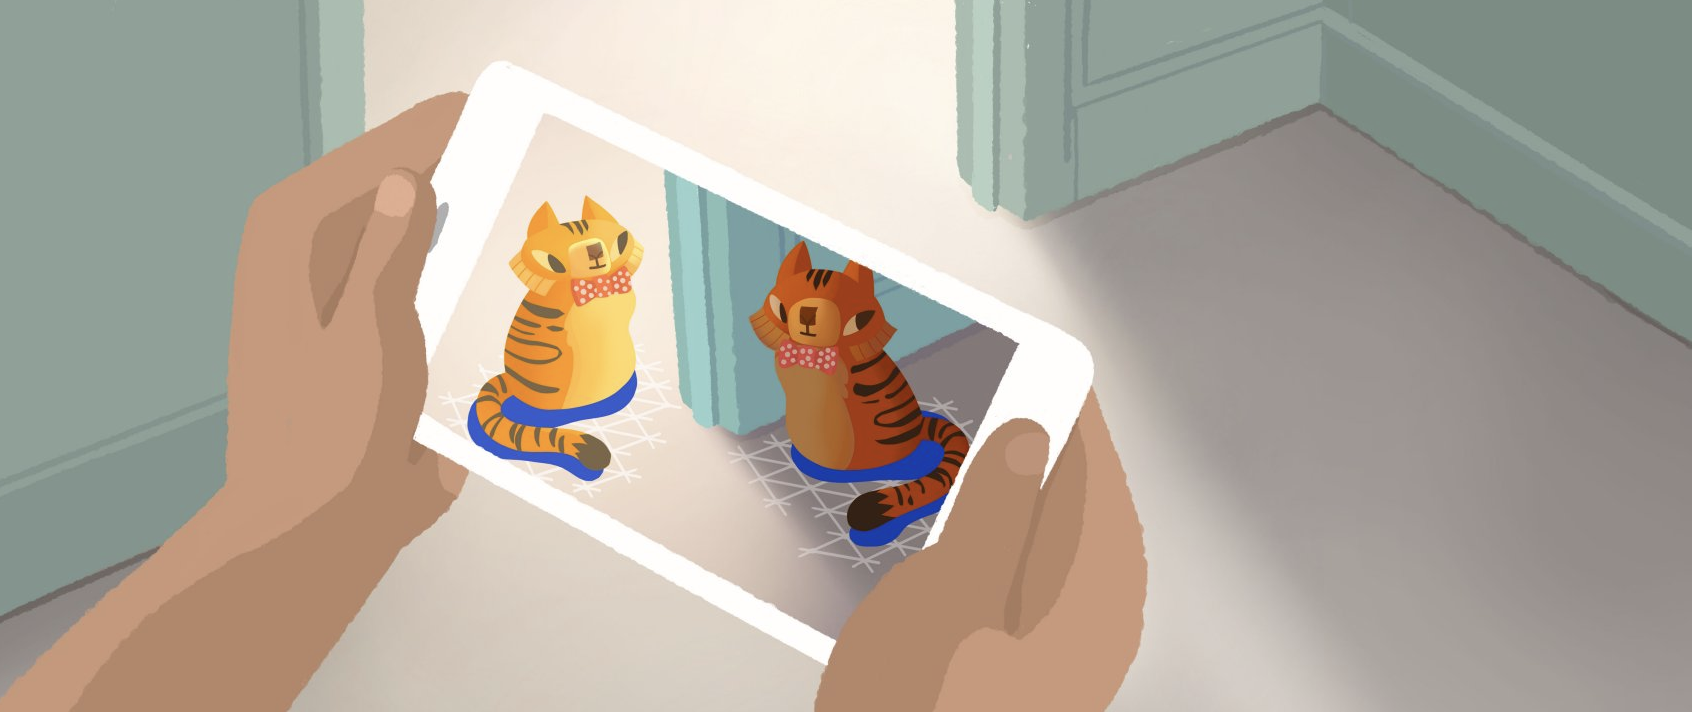
\includegraphics[width=15cm,height=5cm,keepaspectratio]{2Grundlagen/Bilder/lightEstim.png}
    \caption{Skizze zu den Lichtverhältnissen des Smartphones \cite{arcoreofficial.2020j}}
    \label{pic:lightestim}
\end{figure}
\subsection{Android Jetpack}
\label{sec:androidjetpack}
Android Jetpack ist eine Ansammlung an Bibliotheken, die es Entwicklern ermöglicht \textit{Best Practices} zu befolgen, 
Boilerplate\footnote{Sind Codeabschnitte, die an mehreren Stellen mit wenigen oder gar keinen Änderungen aufgeführt sein müssen. \cite{boilerplate.2019m}}-Code 
zu reduzieren und Quell-/ Source-Code zu schreiben. Die durch Android Jetpack zur Verfügung gestellten Bibliotheken fördern die konsistente Funktionsweise der 
Android-Versionen und -Geräten. Darüber hinaus wird mit Android Jetpack ein Überblick verschafft, um Best Practices und empfohlene 
Architekturen zu berücksichtigen.
\\ 
Außerdem wurde Android Jetpack für moderne Design-Praktiken entwickelt, darunter fällt \textit{„seperation of concerns“}\footnote{(SoC), Entwurfsprinzip, um verschiedene Verantwortlichkeiten auf 
verschieden Abschnitte zu trennen. \cite{soc.2019a}}, \textit{testability}, \textit{loose coupling}, \textit{Observer Pattern}\footnote{Beobachter-Muster, Verhaltensmuster der GoF-Muster}, 
\textit{Inversion of Control}\footnote{(IoC), Umsetzugsparadigma, das ein spezifisches Objekt über ein mehrfach verwendetes Objekt aufruft. \cite{ioc.2020}} und 
\textit{productivity features}, z.B. Plugin-Integrationen. Dies sind Techniken, um eine robuste und qualitativ hochwertige App zu erstellen.
\\ 
Die Bibliothekensammlung ist die Grundlage für die verwendete Architektur, Android Architecture Components in Abschnitt \ref{chap:AAC}.
\\ 
\linebreak
Die Abbildung \ref{pic:androidjetpackcomp} zeigt einen Überblick über die in Jetpack enthaltenen Bibliotheken. % in Abschnitt \ref{chap:AAC}
\begin{figure}[hbt!]
    \centering
    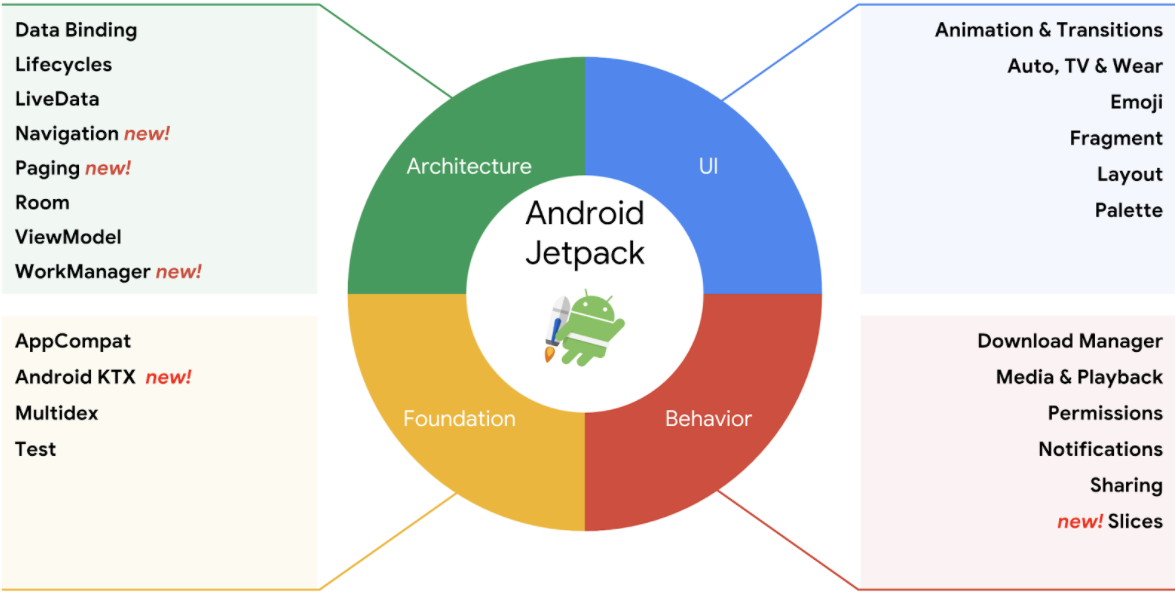
\includegraphics[width=15cm,height=10cm,keepaspectratio]{2Grundlagen/Bilder/androidjetpackcomps.png}
    \caption{Komponenten von Android Jetpack \cite{androidjpdescr.2018m}}
    \label{pic:androidjetpackcomp}
\end{figure}
\\
Eine nähere Erläuterung aller Bibliotheken findet im Rahmen dieser Ausarbeitung nicht statt, wobei die zur Verwendung geplanten 
„Architecture Components“ beschrieben werden. 
\\ 
\linebreak
LiveData, Room und ViewModel sind Bestandteil der \textit{Android Architecture Components}-Konstellation 
und bilden die Basis für die Architektur, welche an das \textit{MVVM-Pattern} angelehnt ist.

\subsection*{LiveData}
\label{sec:LiveData}
\textit{LiveData} gehört zu den \textit{Observer-Pattern} und ist eine Datenhalterklasse die eine Beobachtungsfunktion, bzw. -charakter besitzt. Der 
Unterschied zu einem regulären Observable ist, die lebenszyklus-unabhängige LiveData-Komponente. Dies bedeutet, der Lebenszyklus anderer 
Komponenten z.B. \textit{Activities, Fragments oder Services}, wird berücksichtigt. Mit dieser Kenntnis wird sichergestellt, dass LiveData 
nur App-Komponenten beobachtet, welche sich in einem aktiven Lebenszyklus befinden.
\\ 
\linebreak
Vorteile die die \textit{LiveData}-Komponente mit sich bringt sind unter anderem die Sicherstellung der Übereinstimmung der Benutzeroberfläche und 
deren Datenstatus, vorbeugend gegenüber Speicherverlust, immer auf dem aktuellsten Stand der gespeicherten Informationen und der Wegfall 
der manuellen Lebenszykluskoordination. \cite{livedata.2020}
\subsection*{Room}
\label{sec:Room}
\textit{Room} ist eine Persistenzbibliothek und bietet ein Abstraktionsschicht über der eigentlichen \textit{\acs{SQL}ite}-Datenbank, um einen 
robusten Datenbankzugriff zu managen und das volle Potential von \acs{SQL}ite gleichzeitig zu nutzen. \cite{room.2017}
\\ 
\linebreak
Die robuste \acs{SQL}-Objektzuordnungsbibliothek \textit{Room} kann einen Cache mit den Daten der Applikation auf einem Gerät erstellen. Dieser 
Cache dient als Wahrheitsquelle der Applikation und ermöglicht den Benutzern eine konsistente Kopie der Informationen der App anzuzeigen 
und immer zugänglich zu machen. \textit{Room} kann in drei Kategorien, bzw. in drei Hauptkomponenten unterteilt werden:
\begin{itemize}
    \item Room database: Dient als Zugriffspunkt für die zugrundeliegende SQLite-Datenbank
    \item DAO (Data Access Object): Beinhaltet Methoden um Datenbankzugriffe zu gewährleisten.
    \item Entity: Repräsentiert ein Objekttabelle der Datenbank.
\end{itemize}
Das Diagramm \ref{pic:roomarchitecturediagramm} veranschaulicht die Interaktion, bzw. Funktionsweisen der Hauptkomponenten.
\begin{figure}[hbt!]
    \centering
    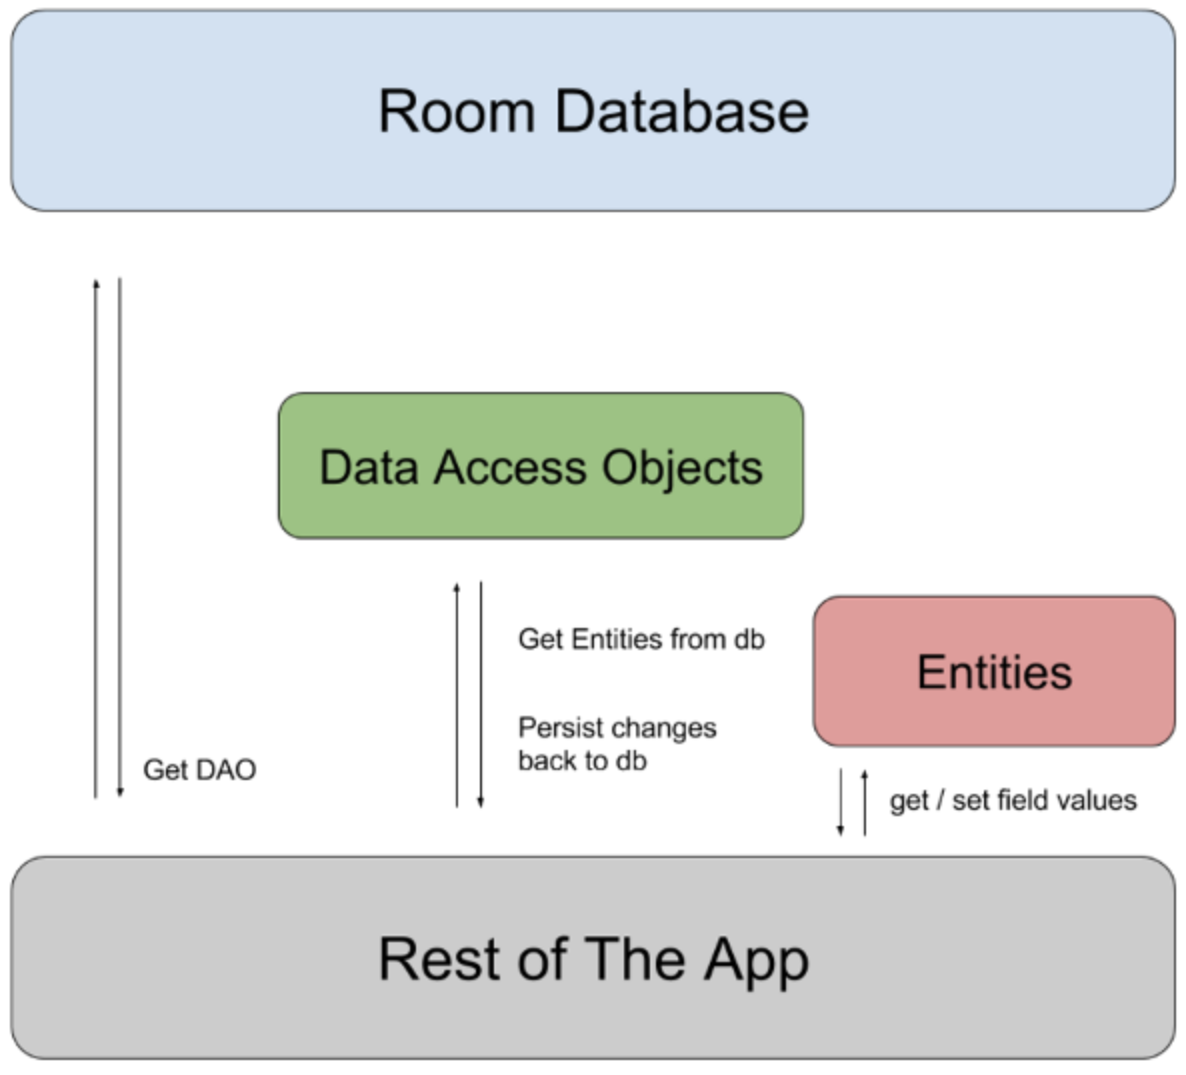
\includegraphics[width=7.5cm,height=7.5cm,keepaspectratio]{2Grundlagen/Bilder/roomArchitecture.png}
    \caption{Room Architektur Diagramm \cite{roomdiagr.2017}}
    \label{pic:roomarchitecturediagramm}
\end{figure}
\\ 
%\pagebreak
\linebreak
Allgemein ermöglicht \textit{Room} einen vereinfachten Zugriff auf die Datenbank, hat einen hohen Grad an \textit{„testability“}, zur 
Kompilierungszeit wird eine \acs{SQL}-Abfrageüberprüfung durchgeführt und interagiert einwandfrei mit anderen Android Architecture 
Components, z.B. LiveData und ViewModel.

\subsection*{ViewModel}
\label{sec:ViewModel}
Grundsätzlich dient das \textit{ViewModel} als lebenszyklusbewusste Speicherung und Verwaltung von benutzeroberflächenbezogenen Daten. 
Durch die \textit{ViewModel}-Klasse können Informationen Konfigurationsänderungen, z.B. Bildschirmdrehungen, die als Änderung zählen, 
überstehen. Eine Konfiguration kann sog. Activities verwerfen und neu laden, so können nicht persistierte Daten verloren gehen. 
\\ 
\linebreak
Ein \textit{ViewModel} fungiert ebenso als Kommunikationsschnittstelle zwischen den darüber- und darunterliegenden Komponenten der 
Architektur (siehe Abschnitt \ref{chap:AAC}). Des Weiteren kann die \textit{ViewModel}-Komponente Informationen zwischen Benutzeroberflächen 
und verschiedenen Fragmenten, engl. \textit{„fragments“}\footnote{Teil einer \ac{UI} in einer Android Activity}, teilen.
\\ 
\linebreak
Die Abbildung \ref{pic:viewModeldiagramm} zeigt eine sich ändernde Activity, die zu Beginn und nach Neuerstellung oder Aktualisierung Zugriff 
auf die unveränderten Daten hat. 
\begin{figure}[hbt!]
    \centering
    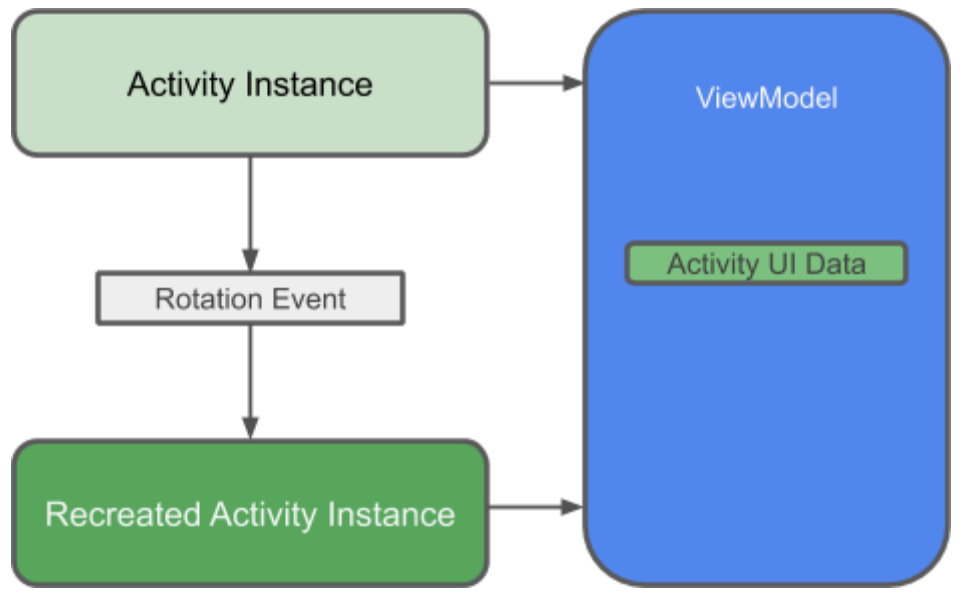
\includegraphics[width=7.5cm,height=7.5cm,keepaspectratio]{2Grundlagen/Bilder/viewModelDiagram.png}
    \caption{ViewModel Struktur Diagramm \cite{viewmodeldiagr.2020}}
    \label{pic:viewModeldiagramm}
\end{figure} 
\pagebreak
\subsection{Sceneform SDK}
Das Sceneform \acs{SDK} ist ein Open-Source Projekt der Google LLC., welches für das Rendern von 3D-Szenen und -Animationen zuständig ist. 
Basierend auf der physikalischen Echtzeit-Rendering-Engine, \textit{physically based renderer} für Android, iOS, macOS, Linux und Windows 
von Google Filament, wurde Sceneform entwickelt. 
\\ 
\linebreak
Bei dem Ansatz des physikalisch basierten Renderns in der Computergrafik wird versucht, alle Modalitäten der realen Welt genauer zu modellieren. 
Mit dieser Methode werden virtuelle 3D-Objekte in der \acl{AR} noch realer dargestellt, um einen Echtheitseffekt zu erzielen und zu simulieren. 
Ein Beispiel ist das Simulieren des Lichtflusses, um einen Schatten des Objekts zu erzeugen, wodurch die Wirksamkeit immer mehr der Realität 
entspricht.
\\ 
\linebreak
Dreidimensionale Modelle werden als \textit{(.obj)}-Dateien in das Projekt importiert. Diese Dateien beinhalten aufgelistete Punkte, Vektoren 
und Linien, welche das Modell repräsentieren. Das \textit{Sceneform \acs{SDK}} verwendet die \textit{.obj}-Datei und konvertiert, bzw. 
rendert diese in eine, \textit{Sceneform binary assets (.sfb)}-Datei. Diese generierte Datei ermöglicht das Generieren eines dreidimensionalen 
Objekts, welches anschließend in \acs{AR}-Anwendungen basierend auf Google ARCore verwendet werden kann. 
Für die finale Renderung und Anzeige ist die \textit{ModelRenderable}-Klasse des \acs{SDK}s zuständig. 
%\\ 
%\linebreak
%Ein weiterer wichtiger Aspekt diese Projekts ist der Einsatz einer Datenbank, um generierte Daten speichern zu können.
\subsection{SQLite}
\acs{SQL}ite ist eine Open-Source In-Process-Bibliothek, die ein in sich geschlossenes, serverloses, transaktionsfreies \acs{SQL}-Datenbankmodul 
ohne Konfiguration implementiert. \acs{SQL}ite ist eine eingebettete \acs{SQL}-Datenbank-Engine die im Gegensatz zu anderen \acs{SQL}-Datenbanken über 
keinen separaten Serverprozess verfügt, d.h. Transaktionen, Lese- und Schreibzugriffe werden direkt auf eine normale Festplattendatei getätigt. \cite{sqlite.2018j}
\\
Darüber hinaus ist \acs{SQL}ite plattformübergreifend und kann beliebig Datenbank- und Objekttabellen, Indizes und Ansichten erstellen und verwalten. 
% %%%%%%%%%%%%%%%%%%%%%%%%%%%%%%%%%%%%%%%%%%%%%%%%%%%%%%%%%%%%%%%%%%%%%%%%%%%%%
%% Descr:       Vorlage für Berichte der DHBW-Karlsruhe, Ein Kapitel
%% Author:      Prof. Dr. Jürgen Vollmer, vollmer@dhbw-karlsruhe.de
%% $Id: kapitel2.tex,v 1.5 2017/10/06 14:02:51 vollmer Exp $
%%  -*- coding: utf-8 -*-
%%%%%%%%%%%%%%%%%%%%%%%%%%%%%%%%%%%%%%%%%%%%%%%%%%%%%%%%%%%%%%%%%%%%%%%%%%%%%%%

%\section{OpenGL}
%\label{chap:OpenGL}
%\subsection{Projektionen}
%\subsection{Shader}

\section{Softwarearchitektur}
\label{chap:Softwarearchitektur}
Komponenten in Form von Klassen, Objekten oder Bibliotheken und deren Verbindungen zwischen einzelnen Komponenten beschreibt die Architektur 
eines Softwaresystems. Vielmehr geht es bei der Software-Architektur darum, Anforderungen und deren Zusammenhänge untereinander von dem zu 
konstruierenden System zu beschreiben und nicht einen detaillierten Entwurf vorzulegen. Jedoch hat die Architektur einen enormen Einfluss 
auf die qualitativen und nicht-funktionalen Eigenschaften des daraus resultierenden Systems. 
\\ 
\linebreak
Die Terminologie nach dem \textit{IEEE-Standard 1471-2000} zur Software Architekturbeschreibung, deren Aufgaben und Zweck \cite{swarchitekturieee.2005} 
sind wie folgt definiert: 
\begin{quote}
    Die grundlegende Organisation eines Systems, dargestellt durch dessen Komponenten, deren Beziehungen zueinander und zur Umgebung sowie den 
    Prinzipien, die den Entwurf und die Evolution des Systems bestimmen. \cite{architektursw.2006f}
\end{quote}
Softwarearchitektur bietet viele Möglichkeiten, ein System zu entwerfen und Anforderungen und Eigenschaften umzusetzen. Daher gibt es auch 
hier viele Ansätze, Lösungen und Abwandlungen, um den Standards und Richtlinien gerecht zu werden. Beispiele dafür sind unter anderem die 
Modulare Software Architektur (\ref{chap:Modulare Software Architektur}) und das Architektur-Entwurfsmuster MVVM (\ref{chap:MVVM}).
\\
Das Buch \textit{Design Patterns - Elements of Reusable Object-Oriented Software} von E. Gamma, R. Helm, R. Johnson und J. Vlissides befasst 
sich mit den verschiedensten Möglichkeiten und Ausprägungen der Softwarearchitektur. 
\\ 
Im Rahmen dieser Ausarbeitung findet keine Aufzählung und Beschreibung verschiedener Arten der Architekturmuster und -stile statt, lediglich die 
für das Projekt verwendeten Muster werden in folgenden Kapiteln aufgegriffen. 
\\ 
\linebreak
Die Abbildung (\ref{pic:mvcdiagram}) veranschaulicht eine vereinfachte Struktur eines Architekturmusters und deren Komponenten und Zusammenhänge 
zueinander. Die Zeichnung dient zur Veranschaulichung, um darzulegen, wie ein Architekturdiagramm aussehen kann, bzw. wie die allgemeine 
Struktur repräsentiert wird.
\begin{figure}[hbt!]
    \centering
    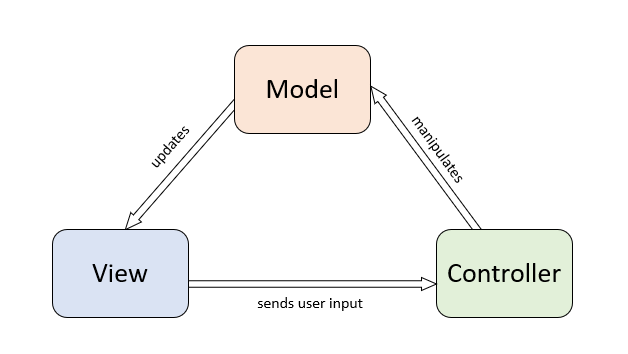
\includegraphics[width=15cm,height=7.5cm,keepaspectratio]{2GrundlagenX/Bilder/MVCArchitecture.png}
    \caption{MVC Architektur Diagramm \cite{mvcbild.2020}}
    \label{pic:mvcdiagram}
\end{figure} 
\\
Im Falle dieser Abbildung wurde das Strukturmuster \ac{MVC} ausgewählt, welches die zu sehenden Komponenten in drei in sich 
geschlossene und unabhängige miteinander agierende Fragmente unterteilt. 
\\ 
\linebreak
Neben der Strukturierung von Systemen und Applikationen kann die Modellierung einer Softwarearchitektur auch dabei helfen, eine Architektur genauer 
zu beschreiben und zu dokumentieren. Ebenso können Diagramme auch das Management sowie die Planung beeinflussen und verstärken. Die Modellierung 
der Softwarearchitektur stellt somit keinen Selbstzweck dar, sondern bietet einen Mehrwert, weil es zur Verständigung, Dokumentation und 
Kommunikation zwischen Entwicklern und Kunden zusätzlich beiträgt. 
\\ 
Durch die Modellierung der Architektur kann frühzeitig eine sinnvolle Evaluierung und Bewertung des Entwurfs durchgeführt werden. Mit diesen 
entstehenden Bewertungen können folgende Schritte besser geplant und umgesetzt werden. 
\\ 
\linebreak
Eine weitere Variante, bzw. Ausprägung der Software-Architektur ist die Modulare Software-Architektur (siehe Abschnitt \ref{chap:Modulare Software Architektur}).
Viele Softwarearchitekturen lehnen sich an das Prinzip der Modularen Architektur an und nehmen diese als Grundlage.

\subsection{Modulare Software-Architektur}
\label{chap:Modulare Software Architektur}
Der Begriff der Modularität beschreibt den Hauptteil der Architektur. Modularität bezeichnet die Aufteilung eines großen Ganzen in 
mehrere kleinere Teile, die als Module, Komponenten oder Bausteine beschrieben werden. Verschiedene Teile können bei geeigneter Funktion 
und Kompatibilität zusammengeführt werden oder über entsprechend definierte Schnittstellen interagieren. 
\\ 
Unter der allgemeinen modularen Software-Architektur, bzw. Programmierung, versteht man ein Programmierparadigma. Dabei sollte die Software aus 
systematisch und logisch aufgeteilten Teilblöcken bestehen, diese werden Module oder Bausteine genannt. Der Aufbau der modularen Software kann 
praktisch in allen imperativen Programmiersprachen\footnote{Programmierparadigma, das aus einer Folge von Anweisungen besteht.} 
Anwendung finden. Durch Modularität soll die Software bessere Kontrollierbarkeit, Übersichtlichkeit und Testbarkeit innerhalb großer 
Softwareprojekte gewährleisten. So sind die einzelnen Bausteine an sich unabhängig und für sich selbst zuständig, trotzdem können 
diese mit weiteren Bausteinen kombiniert und verschachtelt werden. 
\\ 
In der Entwicklung sind die einzelnen Module eigenständig und separat zu planen, programmieren und testen. Dadurch ist der Rahmen des 
einzelnen Moduls überschaubar. Nach erfolgreicher Testung der Module können die Einzelteile als eine Anwendung 
zusammengeführt werden, indem sie logisch über Schnittstellen verknüpft werden. Erst nach diesem Schritt ist die 
entstehende Applikation vollständig einsatzbereit.
\\ 
Die modulare Programmierung gilt als Erweiterung des prozeduralen Ansatzes, dabei sind die Module in kleineren Ansätzen auf die Klassen 
der objektorientierten Programmierung zurückzuführen. \cite{modularesoftware.2018s}
\\
Um eine Software-Architektur übersichtlich und strukturiert umzusetzen, gibt es demzufolge Entwurfsmuster, engl. Patterns, die zusätzlich für 
Ordnung innerhalb der Architektur sorgen. Ein für die Ausarbeitung relevantes Muster ist das MVVM-Pattern. (siehe \ref{chap:MVVM})

\subsection{MVVM}
\label{chap:MVVM}
Das Model-View-ViewModel-Pattern ist, wie bereits erwähnt, ein Architekturmuster das den Entwicklern als Vorlage dient, um ordnungsgemäße, 
standardisierte und strukturierte grafische Oberflächen und das dahinterstehende logische System zu entwickeln. Es wird besonders für 
interaktive Systeme eingesetzt. Das MVVM-Muster wird allgemein als Weiterentwicklung des bekannten MVC-Patterns (der Abbildung \ref{pic:mvcdiagram} zu entnehmen) angesehen. 
\\
Grundlegend ist das Model-View-Controller-Muster, MVC, für die klare Abgrenzung zwischen dem Datenmodell, der Darstellung von Daten und der Steuerung von 
Nutzerinteraktionen zuständig. Der Controller koordiniert die Aktionen der View und dem Model. Dieser fungiert als Verbindungsstück zwischen den Bestandteilen und informiert 
die View im Bedarfsfall bei Änderungen am Model. 
\\ 
\linebreak
Demnach ist auch das Model-View-ViewModel-Muster daran angelehnt, die Benutzeroberfläche von deren Logik zu trennen. Durch diese Trennung 
ist eine erhöhte Wart- und Testbarkeit gewährleistet. Die ermöglichte parallele Arbeitsweise von UI-Designern und Entwicklern 
unterstützt deren Arbeitsfluss und beschleunigt den Entwicklungsprozess. \cite{mvvmentwickler.2010s} 
\\ 
\linebreak
Die Logik der Anwendung wird in den ViewModel-Klassen (\ref{sec:ViewModel}) dargestellt und dienen als Kommunikationsschnittstelle zwischen 
dem Model, dem Datenhalter und der View, der Datenrepräsentation. Durch die Unabhängigkeit der einzelnen Module kann ein Unit Test vereinfacht 
durchgeführt werden, mitunter ein großer Vorteil des Patterns. 
\\ 
Die Ebenen, die das MVVM-Pattern enthält, werden in Abbildung (\ref{pic:mvvmdiagram}) grafisch aufgeführt.
\begin{figure}[hbt!]
    \centering
    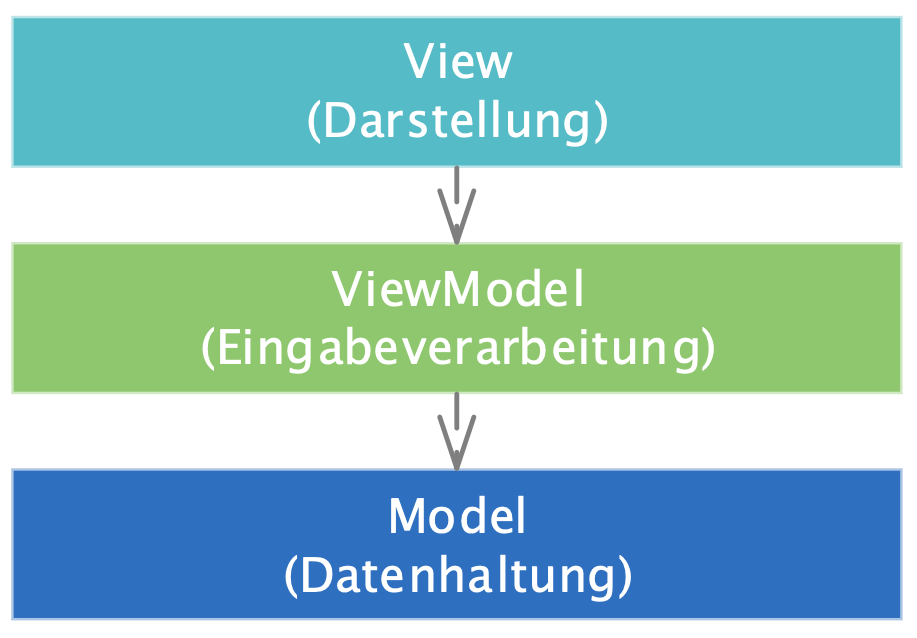
\includegraphics[width=15cm,height=7.5cm,keepaspectratio]{2GrundlagenX/Bilder/mvvmDiagramm.png}
    \caption{MVVM Architektur Diagramm \cite{mvvmDiagramm.2015n}}
    \label{pic:mvvmdiagram}
\end{figure} 
\\
Die View-Ebene stellt die Informationen der Benutzeroberfläche dar, fängt die Benutzereingaben ab 
und gibt diese über Datenbindungen dann an das darunterliegende ViewModel weiter. Die View-Klasse enthält lediglich die Komponenten, die 
die Oberfläche optisch ausmachen und die dazugehörigen Datenbindungsschnittstellen bereitstellt, um die Informationen übergeben zu können.
Ebenso werden über diese Schnittstellen Informationen geladen, um diese auf der Oberfläche repräsentieren zu können. 
Diese Vorgehensweise erleichtert das Austauschen der View, ohne den Code generell zu ändern. 
\\ 
\linebreak 
Die ViewModel, bereits in Kapitel (\ref{sec:ViewModel}) beschrieben, ist dafür zuständig, die Daten zwischen der persistierten Speicherung 
und der Repräsentation zu transferieren. Es stellt das Model für die View dar und gibt das eigentliche Model nach außen.
\\ 
\linebreak 
Die unterste Ebene, das Model, bzw. die Datenhaltung, stellt die Abbildung der Daten dar und gilt nicht als reine Abbildung der Datenquelle. 
Diese Daten werden für die visuelle Anwendung auf der View-Ebene benötigt und durch die ViewModel-Ebene bereitgestellt. Darüber hinaus können die 
Daten von dem Nutzer über die View manipuliert und an das Model zurückgegeben werden. Durch diese Möglichkeiten ist vorausgesetzte, dass das Model 
folgende Funktionalitäten bereitstellen sollte \cite{mvvmAufbau.2016}:
\begin{itemize}
    \item Validierung der Daten
    \item  Benachrichtigung bei Eigenschafts-Änderungen
    \item Verarbeitung von Business-Rules
\end{itemize} 
Sozusagen dient das Model als Schnittstelle zwischen der anhängenden Datenbank und dem ViewModel, welches die Daten hält. 
Dazu kommt, dass das Model festlegt, wie die Objekte aufgebaut sind, d.h. dort wird festgelegt, welche Informationen das Objekt beinhaltet. 
\\ 
\linebreak
Die nachfolgende Abbildung (\ref{pic:infoflussmvvm}) veranschaulicht den Informationsfluss des MVVM-Patterns in einzelnen Schritten.
\begin{figure}[hbt!]
    \centering
    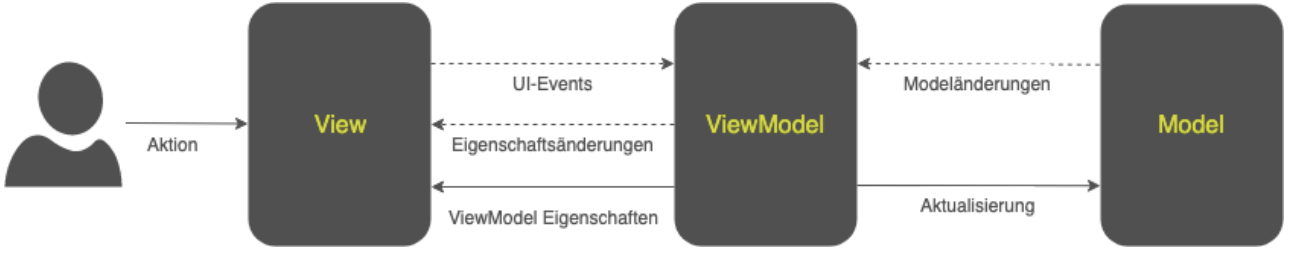
\includegraphics[width=15cm,height=7.5cm,keepaspectratio]{2GrundlagenX/Bilder/infoflussMVVM.png}
    \caption{MVVM Informationsfluss \cite{androidmvvm.2019a}}
    \label{pic:infoflussmvvm}
\end{figure} 
\\ 
Basierend auf der Grundlage des Model-View-ViewModel-Patterns wurde die für das Projekt anvisierte Architektur, Android Architecture Components (\ref{chap:AAC}), 
entwickelt.  

\subsection{Android Architecture Components}
\label{chap:AAC}
Die Android Architecture Components bestehen aus einer Sammlung von Tools und Bibliotheken, engl. Libraries, die entwickelt wurden, um die 
Konstruktion von testbaren und stabilen Android-Apps zu vereinfachen. Mit der Einführung von Android Jetpack (\ref{sec:androidjetpack}) wurden 
viele Komponenten, z.B. Bibliotheken und Frameworks, für die Entwicklung von Apps vereint. In den vielen Bibliotheken, die von Android Jetpack 
zur Verfügung gestellt werden, befinden sich auch die sogenannten \textit{Architecture components}. Diese \textit{Components} unterstützen und 
fördern die Umsetzung der \textit{MVVM} Pattern basierten Architektur (\ref{chap:MVVM}). Die zuvor genannten Bibliotheken ViewModel, LiveData und Room 
sind maßgebliche Bestandteile für die Gestaltung des angestrebten Musters Model-View-ViewModel. 
\\ 
Google selbst empfiehlt im Rahmen der veröffentlichten Dokumentation \textit{„Guide to app architecture“} die Verwendung der \textit{Architecture components}, um 
eine stabile und leistungsfähige Applikation zu designen. Diese basiert auf bewährten Prinzipien, unter anderem dem \textit{seperation of concerns} Prinzip.
\\ 
\linebreak
Folgender Abschnitt befasst sich im Einzelnen mit den Komponenten, die für die \textit{Android architecture} essentiell sind:
\begin{figure}[hbt!]
    \centering
    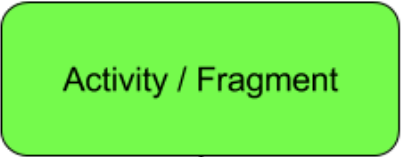
\includegraphics[width=5cm,height=5cm,keepaspectratio]{2GrundlagenX/Bilder/activityComp.png}
    \caption{Android Grundkomponente \cite{aac.2020j}}
    \label{pic:activity}
\end{figure}
\\
Grundsätzlich sind Activities und Fragments nicht Teil der eigentlichen \textit{„Architecture Components“}, sondern sind lediglich Grundkomponenten 
der Android App Entwicklung die die Benutzeroberfläche und die dazu korrespondierenden Layout-Dateien verwaltet. 
\begin{figure}[hbt!]
    \centering
    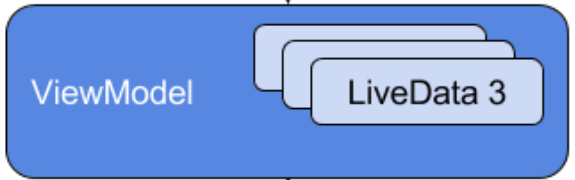
\includegraphics[width=5cm,height=5cm,keepaspectratio]{2GrundlagenX/Bilder/viewModelComp.png}
    \caption{ViewModel Komponente \cite{aac.2020j}}
    \label{pic:vmComp}
\end{figure} 
\\ 
Das ViewModel (siehe Abschnitt \ref{sec:ViewModel}) verwaltet die relevanten Daten der UI. Diese Komponente hat dem Activity-Objekt gegenüber 
einen unabhängigen Lebenszyklus. Somit sind Daten bei unvorhergesehenen Unterbrechungen oder Fehlern der UI nicht betroffen und können bei 
erneutem Aufbau der Oberfläche ohne Probleme nachgeladen werden. Die im ViewModel enthaltenen LiveData Objekte (\ref{sec:LiveData}) sind 
beobachtbare Daten-Container, die eine Activity ohne expliziten Aufruf über Datenänderungen informieren. Durch diese Methode wird der 
Lebenszyklus der aktiven Komponente respektiert und berücksichtigt. 
\begin{figure}[hbt!]
    \centering
    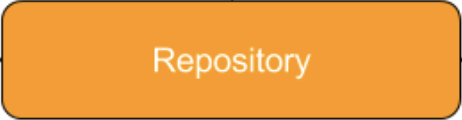
\includegraphics[width=5cm,height=5cm,keepaspectratio]{2GrundlagenX/Bilder/repoComp.png}
    \caption{Repository Komponente \cite{aac.2020j}}
    \label{pic:repoComp}
\end{figure} 
\\ 
Mit dem Repository wird ein „best practice“ Fall umgesetzt, der eigentlich kein Bestandteil der Android Jetpack Library ist. Diese Komponente 
ist dafür zuständig das ViewModel von der eigentlichen Datenquelle zu trennen, um Informationen aus verschiedenen Quellen beziehen und 
synchronisieren zu können. Das Repository dient als Schnittstelle zu mehreren Datenbeziehungspunkten und verwaltet ein Verzeichnis zur 
Speicherung und Beschreibung von Objekten und Informationen. Zudem kapselt das Repositorium die Logik für das Persistieren und Erzeugen von 
Entitäten und Aggregaten von der Ansicht. 
\begin{figure}[hbt!]
    \centering
    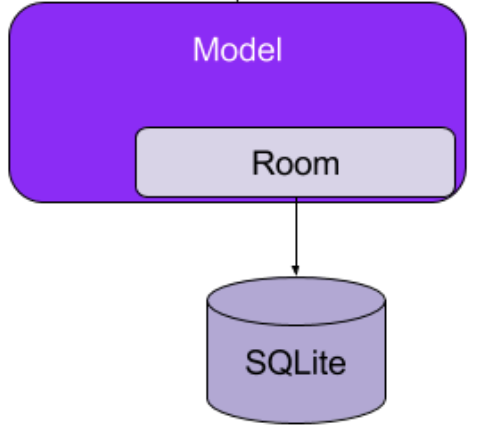
\includegraphics[width=5cm,height=5cm,keepaspectratio]{2GrundlagenX/Bilder/roomComp.png}
    \caption{Model / Room Komponente \cite{aac.2020j}}
    \label{pic:roomComp}
\end{figure} 
\\ 
\linebreak
Die \textit{Persistence Library} Room (\ref{sec:Room}) ist ein Datenbank \textit{Layer} auf der eigentlichen SQLite Datenbank. Zugriffe auf 
die Datenbank werden durch Room gekapselt und vereinfacht, indem viel mit Annotationen, z.B. Entities \textit{(\@Entity)} und Data Objects 
\textit{(\@Dao)}, gearbeitet wird. Der Abbildung (\ref{pic:roomComp}) ist demnach zu entnehmen, dass die Bibliothek \textit{„Room“} einen Großteil der 
Funktionen eines Models abdeckt und so die Model-Komponente repräsentiert. Unter diesem Datenbank Layer befindet sich die eigentliche 
Persistenzschicht, die SQLite Datenbank.  
\\ 
\linebreak 
In einem fortlaufenden Architektur-Diagramm sind die Komponenten wie folgt angeordnet, um die Abhängigkeiten zwischen den einzelnen Teilen 
zu verdeutlichen. 
\begin{figure}[hbt!]
    \centering
    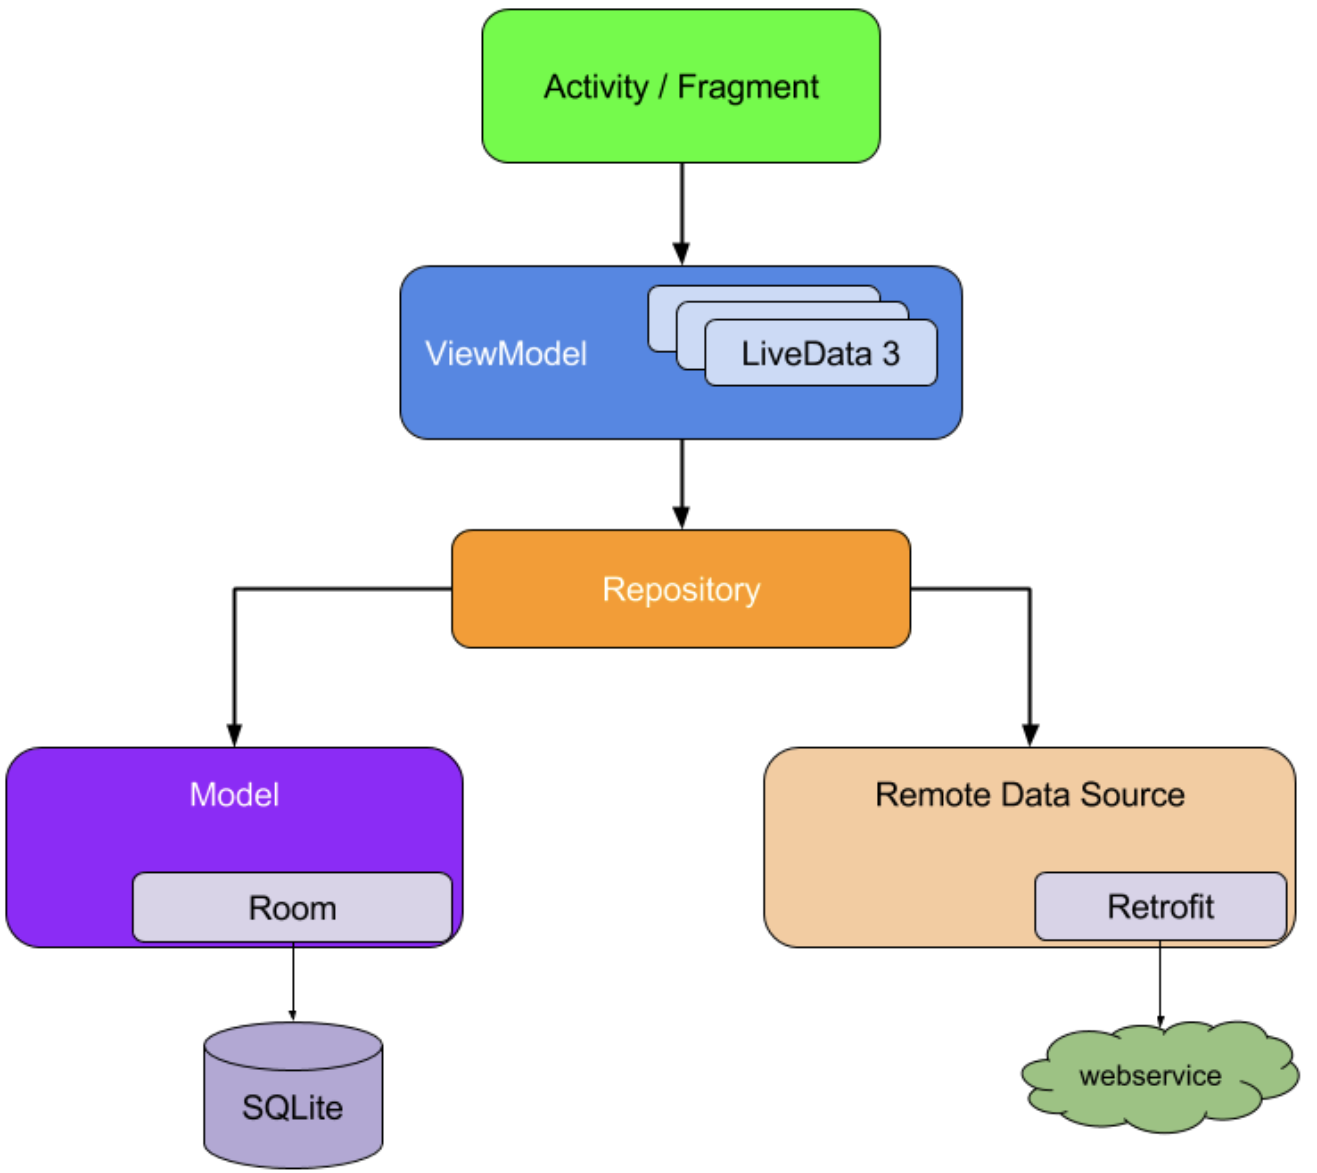
\includegraphics[width=15cm,height=10cm,keepaspectratio]{2GrundlagenX/Bilder/aac.png}
    \caption{Android Architecture Components Diagram\cite{aac.2020j}}
    \label{pic:aacDia}
\end{figure} 
\\ 
In der Abbildung (\ref{pic:aacDia}) wird deutlich, welches Modul welche Abhängigkeiten besitzt, bzw. von welchen Modulen 
Informationen bezogen werden können. Einzelne Komponenten können ihren Vor- oder Nachgänger niemals umgehen und sind so einer festen 
Hierarchie eingeordnet. Die Abbildung zeigt auch eine beispielhafte Ausführung mehrerer Datenbezugsquellen.
\\ 
Bei genauer Betrachtung des Diagramms sind alle Komponenten wiederzufinden, die ebenso in dem MVVM-Muster gegeben 
sind und das Muster prägen. Durch die vielen Komponenten und Schnittstellen, die dazu beitragen, dass weitere Module angehängt oder 
ausgetauscht werden können, ist Modularität gewährleistet. 

\section{Datenmodellierung}
\label{chap:Datenmodellierung}
Datenmodellierung ist ein Verfahren zur formalen Abbildung von Objekten, deren Attribute und Beziehungen in einem definierten Kontext stehen. 
Die Modellierung verfolgt dasZiel, den Überblick über die Daten oder die Applikation zu erhalten. Hauptaufgabe ist die eindeutige 
Definition von Objekten und deren Spezifikationen und Ausprägungen. Ebenso hilft die Datenmodellierung bei der visuellen Darstellung von 
Informationen und bei der Einhaltung von Voraussetzungen und Richtlinien.
\\ 
Die aus der Modellierung entstehenden Datenmodelle stellen die Objekte und Beziehungen untereinander dar und repräsentieren die zu 
persistierende Struktur der Objekte. Datenmodelle sind ein wichtiger Bestandteil einer Software und haben meist eine längere Lebensdauer als 
die Software an sich, da Änderungen an den Modellen meist viele Risiken, dazu zählt überwiegend der Datenverlust, mit sich bringen.
\\ 
\linebreak
Durch die Übersichtlichkeit der Datenmodelle können Standardwerte, Semantik, Sicherheit und die Datenqualität gleichzeitig sichergestellt 
werden. Die Konsistenz von Namenskonventionen wird durch die Überschaubarkeit auch leichter überprüfbar. 
\\ 
\linebreak
In der Softwareentwicklung wird die Datenmodellierung als wesentliche Teilaufgabe gesehen, um ein System aufzubauen. Innerhalb des 
Datendesigns gibt es drei wichtige Varianten, die aufeinander aufbauen:
\pagebreak
\begin{itemize}
    \item Konzeptionelles Datenbankschema: Betrachtung eines für die Applikation wichtigen Szenarios der realen Welt unter Berücksichtigung 
    aller relevanten Objekte, Eigenschaften und Beziehungen zwischen ihnen. Diese Informationen werden aus dem Kontext heraus analysiert 
    und grafisch als auch textuell dargestellt. Die Darstellung basiert auf einem \ac{ERM}, das die Objekte (Entities) mit ihren jeweiligen 
    Eigenschaften (Attributes) und die Beziehungen (Relationships) darstellt. Das ist das sogenannte Semantische Datenmodell.
    \item Logisches Datenbankschema: Hierbei wird das konzeptionelle Datenbankschema um datentechnische Angaben, z.B. Feldtypen /-formate 
    und Identifikationseigenschaften (Primary Keys), erweitert. Das logische Datenbankschemata unterliegt den Regeln der von dem \ac{DBMS}
    gegebenen Struktur, z.B. dem relationalen Datenmodell, das alle Daten und Objekte in Tabellen ablegt. Dies wird auch relationales oder 
    objektorientiertes Datenmodell genannt. \cite{datenmodellierung.2019d}
    \item Physisches Datenbankschema: Dabei werden die Datensätze auf den physischen Komponenten organisiert und verwaltet. Eine Festlegung 
    der Zugriffsoperationen finden in dieser Phase statt. Zugriffsoperationen sind Einfügen, Löschen, Aktualisieren und Suchen von Objekten 
    und Informationen. Zudem wird hierbei versucht, die Performance und effiziente Bearbeitung von Datenbankzugriffen durch Modellierung hochzuhalten.
\end{itemize}  
Die drei oben aufgeführten Phasen sind Bestandteile der Methodik des Datenbankdesigns, der sogenannten \textit{„top down-Methodik“}. 
Wobei die erste Phase die allgemeine Anforderungsanalyse, die in obiger Auflistung nicht aufgeführt ist, beinhaltet. Bei dieser Phase finden 
grundlegende Anforderungsprozesse statt, zum einen die Informationsstrukturanforderungen und zum anderen die Datenverarbeitungsanforderungen. 
\\ 
\linebreak
Ein Schema, nachdem relationale Datenbanken aufgeteilt werden, ist die sogenannte Normalisierung von Datenbanken. Darunter versteht man die 
Aufteilung von Attributen in mehrere Relationen (Tabellen) mithilfe von Normalisierungsregeln und Normalformen. \cite{normalisierung.2020j} 
Ziel dieser Zerlegung ist die Erstellung einer redundanzfreien Speicherung der Daten, um Daten löschen zu können, ohne einen 
Informationsverlust zu erleiden. Die Normalisierung wird in mehrere Stufen unterteilt:
\begin{itemize}
    \item Nullte Normalform (0NF)
    \item Erste Normalform (1NF)
    \item Zweite Normalform (2NF)
    \item Dritte Normalform (3NF)
    \item Boyce Codd Normalform (BCNF)
    \item Vierte \& Fünfte Normalform (4NF \& 5NF)
\end{itemize} 
Die meist verwendete Normalform ist die dritte Normalform, da diese für die Balance zwischen Redundanz, Performance und Flexibilität 
entscheidend ist und oft ausreicht. 
\\ 
Im Folgenden wird nicht weiter auf die Normalformen eingegangen, sie dienen lediglich der vollständigen Nennung. 
% %%%%%%%%%%%%%%%%%%%%%%%%%%%%%%%%%%%%%%%%%%%%%%%%%%%%%%%%%%%%%%%%%%%%%%%%%%%%%
%% Descr:       Vorlage für Berichte der DHBW-Karlsruhe, Ein Kapitel
%% Author:      Prof. Dr. Jürgen Vollmer, vollmer@dhbw-karlsruhe.de
%% $Id: kapitel2.tex,v 1.5 2017/10/06 14:02:51 vollmer Exp $
%%  -*- coding: utf-8 -*-
%%%%%%%%%%%%%%%%%%%%%%%%%%%%%%%%%%%%%%%%%%%%%%%%%%%%%%%%%%%%%%%%%%%%%%%%%%%%%%%

\chapter{Konzeption}
\label{chap:Konzeption}
In diesem Kapitel wird das erarbeitete Konzept dieser Ausarbeitung dargelegt. Dazu gehören die Überlegungen zu einzelnen 
Arbeitsschritten und dem grundsätzlich angedachten Aufbau des Projekts, sowie Entscheidungs- und Beweggründe, weshalb bestimmte 
Technologien gewählt wurden. Zu Beginn wird auf die Einsatzmöglichkeiten (\ref{chap:Arbeitsumgebung}), in der die Applikation Anwendung 
finden könnte, eingegangen. Anschließend werden die Grundgedanken zu den einzelnen Phasen, Scan-Phase (\ref{chap:Scan-Phase}) und 
Visualisierungs-Phase (\ref{chap:Visualisierungs-Phase}) des Systems erläutert, ebenso was sie beinhalten und wie sie funktionstechnisch 
angedacht sind. Mit den zugrundeliegenden Informationen wird auf das Architekturkonzept (\ref{chap:Architekturkonzept}), sowie auf das 
Softwarekonzept (\ref{chap:Architekturkonzept}) eingegangen. Des Weiteren werden die Hintergründe der Wahl des AR-Frameworks 
(\ref{chap:Auswahl des AR Frameworks}) aufgezeigt. Abschließend wird noch das konzipierte und prototypische Datenmodell 
(\ref{chap:Datenmodell}) dargelegt.

\section{Anwendungsumfeld}
\label{chap:Arbeitsumgebung}
Bei der Konzeption wurde darauf Rücksicht genommen, die Anwendung möglichst so zu planen, dass der Einsatzort zu Anfang nicht zwingend 
maßgeblich ist. Dies bedeutet, dass je nach Anwendungsfall die Applikation angepasst werden kann. Allerdings sind für das 
Unterstützungssystem ausschließlich Produktionshallen, eventuell auch Logistik- oder Lagerhallen, vorgesehen. Durch die individuelle 
Möglichkeit des Umgebungsscans ist die Applikation anfangs nicht an festgelegte Orte gebunden. Damit wird zum Ausdruck gebracht, dass der 
Umgebungsscan flexibel durchgeführt werden kann, da keine Anforderungen an die Umgebung gestellt sind. Die darauf aufbauende 
Visualisierungs-Phase ist demnach abhängig von dem Ort, indem der Scan durchgeführt wurde und kann nicht anderweitig, in anderen Hallen, 
eingesetzt werden. 
\\ 
\linebreak
Ein mögliches Anwendungsumfeld dieser Applikation wären die Räumlichkeiten des nahe bei cjt Systemsoftware AG angesiedelten Unternehmes Siemens AG. Neben 
der Vielzahl an gemeinsamen Projekten, wäre dies eine weitere Kooperation mit der Siemens AG und würde eine unterstützende Maßnahme einleiten. 
\pagebreak
\section{Scan-Phase}
%Objekterkennung /
\label{chap:Scan-Phase} %der Aufgabe
Die Definition der Scan-Phase ist entscheidend für die Konzeption und Umsetzung der Architektur- und Softwarekonzeption. 
Anhand der dabei entstehenden Anforderungen und Zielsetzungen konnte die Konzeption ausgelegt und erarbeitet werden. Dieser Abschnitt widmet 
sich der expliziten theoretischen Erläuterung dieser Phase und somit auch einer der beiden Kernfunktionen dieses Softwaresystems.
\\ 
\linebreak
Der Nutzer hält ein Smartphone oder Tablet in der Hand und steht am Eingang der Räumlichkeit. An diesem Punkt wird der Scan-Vorgang gestartet. 
Mittels Smartphone-Kamera hat der Nutzer die Möglichkeit, das Umfeld zu scannen. Dabei wird am Anfang der Startpunkt als Nullpunkt, bzw. 
als Ursprungskoordinaten des erstellten Koordinatensystems der Umgebung, festgelegt. Der Nutzer kann sich frei im Raum bewegen und ist lediglich 
durch das Halten des Smartphones eingeschränkt. Während der Aufnahme wird anhand der im Smartphone integrierten Kamera und 
Sensoren unter Verwendung der Sensordaten ein Modell erstellt, welches die Umgebung virtuell repräsentiert. Dabei wird das Modell auf 
einem dreidimensionalen Koordinatensystem widergespiegelt, um Position, Blickrichtung und Höhe des zu erstellenden Objektes festzuhalten. 
So kommt das \acl{SLAM} Verfahren (siehe Abschnitt \ref{chap:SLAM}) zum Einsatz, das das Smartphone genauestens räumlich lokalisiert und 
gleichzeitig mapped. Dies bedeutet, dass anhand der generierten Sensordaten eine Analyse der Informationen stattfindet und daraus eine 
virtuelle Karte des Raums erstellt wird. Dadurch kann das Gerät die Realität wiedergeben. Anhand der Informationen, die durch
Gegenstände, Wände und dem Boden grundlegend gegeben sind, resultieren die Anhaltspunkte der virtuellen Umgebung. 
\\ 
Dem Nutzer soll die Möglichkeit geboten sein, Objekte an denen vom Anwender vorgesehenen Positionen platzieren zu können. Die Objekte werden 
dann, anhand der durch das \acs{SLAM} Verfahren zugrundeliegenden Informationen, an der virtuellen Position erstellt und positioniert. Somit 
stehen Daten über die Position des Objekts zur Verfügung, welche anschließend in der Datenbank persistiert werden. Währenddessen das Objekt 
erstellt wird, kann der Anwender zusätzliche Informationen zu dem Objekt, welches ebenso in der Realität vorhanden ist, einpflegen. Die 
einzutragenden Informationen belaufen sich zu Anfang der prototypischen Konzeption auf den Namen des Geräts, die Position sowie die 
Blickrichtung als auch den aktuellen Zustandsstatus des realen Objekts. Eine eindeutige Identifikationsnummer wird zudem automatisch generiert, 
um eine einheitliche Richtlinie vorzugeben. Damit muss, bzw. soll der Nutzer die Entscheidung nicht selbst treffen. Die genauere Konzeption 
dieses Falls wird in dem Abschnitt Datenmodell (\ref{chap:Datenmodell}) aufgegriffen. 
\\ 
Ziel bei der oben aufgeführten Scan-Funktion ist das Erstellen und Platzieren von virtuellen Objekten in der durch Scans erstellte und 
realitätsnahe Inszenierung des Umfeldes. In überschaubarem Rahmen wurden Anforderungen für die Scan-Phase erarbeitet, unter anderem die 
Einfachheit der Objekterstellung, die simpel und überschaubar zu erstellende Benutzeroberfläche, die offensichtliche Objektdarstellung 
in kurzer Zeit und einen nicht allzu hohen Zeitaufwand.
\\ 
\linebreak
Nachdem die Scan-Phase, eine der beiden Kernfunktionen, konzeptionell präzisiert wurde, kommt nun die Erläuterung der zweiten Kernfunktion, 
die sogenannte Visualisierungs-Phase. 

\section{Visualisierungs-Phase}
\label{chap:Visualisierungs-Phase}
Dieser Abschnitt definiert die Aufgabe der Visualisierungs-Phase. Dabei werden auch hier Anforderungen und Zielsetzungen dieser Funktion 
theoretisch ausgeführt, um die anfänglichen Ideen, womit die allgemeine Konzeption der Software erarbeitet wurde, aufzuzeigen. Dafür ist 
vorauszusetzen, dass die Scan-Phase alle erforderlichen Daten und Informationen liefert. 
\\ 
\linebreak
Diese Funktion ist hauptsächlich zur reinen Darstellung der vorab in der Scan-Phase erstellten Objekte gedacht. Mit diesem Teil des Systems 
kann der Nutzer sich frei im Raum bewegen und bekommt die Objekte in seinem Umfeld auf dem Bildschirm des Smartphones angezeigt. 
Befindet sich ein Objekt in der Nähe, hat der Nutzer die Möglichkeit, durch Anklicken des Objekts genauere Informationen über dieses zu erhalten. 
\\ 
\linebreak 
Startet der Anwender die Methode, werden alle Objekte aus der Datenbank abgefragt und mit dem dazugehörigen Zustandsstatus in den Raum 
projiziert, sodass Auffälligkeiten sofort zu sehen sind. Dies bedeutet, bei normalem, aktivem Status ist die Farbe der Projektion grün, 
bei fehlerhaftem, passivem Status rot. Dadurch wird schnell klar, ob es an bestimmten Objekten in der Realität Probleme gibt. Mithilfe dieser 
Funktion wird im Handumdrehen ein Überblick über die Situation und Lage der Objekte verschafft. Falls es zu einem ungewollten Verhalten kommt, 
kann der Anwender unverzüglich eingreifen und dementsprechend handeln. Wird ein Objekt durch die Kamera 
fokussiert, kann der Anwender das Objekt anklicken, um weitere Informationen über dieses zu erhalten. 
\\ 
Die Visualisierungs-Phase sieht es allerdings nicht vor, während die Applikation läuft, neue Objekte hinzuzufügen. Dafür müsste der Anwender wiederum zur 
Funktion der Scan-Phase wechseln. Eine Änderung an den Objekten selbst kann nur bedingt vorgenommen werden, dies betrifft ausschließlich
Informationsänderungen, die das Objekt selbst betreffen.  

\section{Architekturkonzept}
\label{chap:Architekturkonzept}
Um das \acl{AR} basierte Assistenzsystem grundlegend zu definieren, ist es von Vorteil ein geeignetes Konzept sowie einen ersten Entwurf zu 
erstellen. Dieser sollte als Fundament für eine Applikation mit stetig steigender Anzahl an Funktionen dienen und für künftige Weiterentwicklungen 
verwendet werden. Anfänglich soll der Prototyp dafür sorgen, dem Nutzer einen Überblick über beispielsweise Maschinen in Produktionshallen zu 
verschaffen. Dies bedeutet, dass Informationen zu bestimmten Objekten schnell zur Verfügung stehen und eventuell defekte Maschinen zügig 
aufzufinden sind. Grundsätzlich muss die Anwendung in der Lage sein, auf Benutzerbedienungen zu reagieren, die Umgebung zu scannen, 3D-Objekte 
an der vom Nutzer vorgesehenen Stelle zu platzieren, Informationen zu den jeweiligen Objekten hinzuzufügen und ändern zu können. Wird die 
Applikation gestartet, die Umgebung gescannt und Objekte auf die vom Nutzer vorgesehenen Positionen platziert, sollen die erstellten Objekte 
gespeichert und bei erneutem Start der Anwendung aufgerufen und platziert werden. Neben der \acl{AR} Funktion soll die %alle vorhandenen Objekte
entstehende Software für eine fortlaufende Entwicklung geeignet sein. Für diese Eigenschaft ist ein modularer Architekturansatz vorgesehen, 
um das schnelle und einfache Wechseln von Komponenten und Bestandteilen zu ermöglichen. Darunter sind beispielsweise Änderungen an der 
Benutzeroberfläche oder die Verwendung einer anderen Datenbank, bzw. hinzukommende Funktionen, die unabhängig von bestehenden Klassen 
hinzugefügt werden können. Durch das \acs{MVVM}-Pattern, welches durch die \textit{Android Architecture Components} gefördert wird, ist 
das Testen von \textit{\acs{GUI}}- und \textit{BackEnd}-Elementen unabhängig voneinander begünstigt. 
\\ 
\linebreak
Wie bereits erwähnt, sind die \textit{Android Architectur Components} an das Entwurfsmuster \textit{MVVM} angelehnt und sorgen im Allgemeinen 
dafür, die Software im gesamten überschaubar und beherrschbar zu gestalten. Dabei werden die folgenden Prinzipien beachtet und auch gewährleistet. 
Durch gezielte Abstraktion von Informationen wird die Komplexität einer Anwendung steuerbar. Mit der großen Anzahl an verschiedenen 
Segmenten, die der Abbildung (\ref{pic:architectur}) zu entnehmen sind, wird die Trennung der Zuständigkeit (engl. \textit{seperation of concerns}) 
deutlich. Dabei hat jede einzelne Komponente eine Zuständigkeit, bzw. Aufgabe, die sie zu bewerkstelligen hat. Sei es die \textit{View} 
mit der der Nutzer interagiert, dem \textit{ViewModel} als Kommunikationsschnittstelle, dem %und Zwischenspeicherung von Daten
\textit{Repository} als Verzeichnis zur Speicherung und Beschreibung von Objekten oder als Schnittstelle zu mehreren Datenbeziehungspunkten 
oder das \textit{Model}, das die Zugriffe auf die Datenbank kapselt und die Struktur der Objekte vorgibt. %, bzw. der zu speichernden Daten
Ein weiterer Aspekt ist das daraus resultierende und idealerweise in sich geschlossene System, das durch lose Kopplung und hohe Kohäsion in 
eine Menge an Komponenten zerlegt ist, die dadurch gewonnene Modularität. 
\\ 
\linebreak
Die Software wurde zunächst, den Phasen entsprechend (siehe Abschnitt \ref{chap:Scan-Phase} \& \ref{chap:Visualisierungs-Phase}), in zwei 
große Rubriken, den sogenannten Scan- und Visualisierungs-Phasen, unterteilt. Diese Phasen finden sich in der Abbildung (\ref{pic:architectur}) der 
konzeptionellen Architektur des Unterstützungssystems wieder. 
\\ 
\textit{Views}, bzw. \textit{Activities} werden mithilfe der von Android zur Verfügung gestellten \textit{AppCompat-Library} erstellt. Die 
von Android Jetpack vorhandene Bibliothek ViewModel dient als Kommunikationsschnittstelle zwischen der \acs{GUI} und dem Repository. 
Die ebenso von Android Jetpack publizierte LiveData-Bibliothek gilt als Observer zur \acs{GUI} und benachrichtigt diese bei Änderungen. Mit 
der Repository-Komponente zwischen ViewModel und Datenbank, bzw. Model wird eine reine und neu generierte \acs{API}-Schnittstelle erstellt, 
welche der Benutzeroberfläche Aufrufe für Datenbankzugriffe zur Verfügung stellt. Die Room-Bibliothek stellt ein Zugriffs-Layer da, welches 
die Datenbankzugriffe kapselt und steht gleichzeitig als Model bereit. Dort werden Entities, in der für die Datenbank vorgesehene 
Struktur, festgelegt. Data Objects (DAOs) regeln die Datenbank-Zugriffe über definierte SQL-Queries, die vorab, den Funktionen entsprechend, 
modelliert werden. Um die entstehenden Daten der dreidimensionalen \acs{AR}-Objekte zu speichern wird eine SQLite-Datenbank verwendet.
\begin{figure}[hbt!]
    \centering
    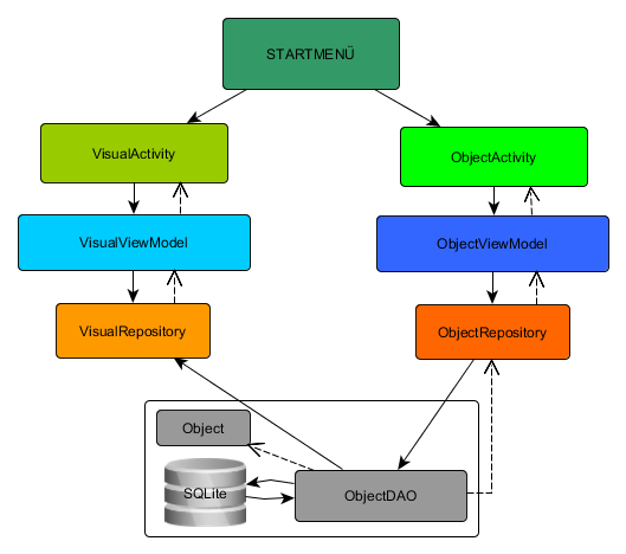
\includegraphics[width=13cm,height=13cm,keepaspectratio]{3Konzeption/Bilder/architektur_konzept.png}
    \caption{Konzeptionelle Software-Architektur}
    \label{pic:architectur}
\end{figure}
\pagebreak
\section{Softwarekonzept}
\label{chap:Softwarekonzept}
Nachdem die Architektur konzipiert und ein grobes Bild des entstehenden Systems geschaffen wurde, konnte die Konzeption des 
Softwaresystems beginnen. In der Konzeption werden die Kernfunktionen, sowie die Anforderungen und Ziele veranschaulicht.
\\ 
\linebreak 
Beim Starten der Applikation öffnet sich das Startmenü der Anwendung. Hier sind auf einen Blick zentral alle Funktionen, die das System 
unterstützt, übersichtlich angezeigt. Dort wird die Möglichkeit offeriert, die Scan-Phase (\ref{chap:Scan-Phase}) zu starten oder fortzuführen 
oder die Visualisierungs-Phase (\ref{chap:Visualisierungs-Phase}) nach erfolgtem Scannen zu starten. Dabei wird auch das Ziel verfolgt, den 
Nutzer nicht mit Informationen zu erschlagen, bzw. den Nutzer nicht unnötig zu verwirren und ohne große Umschweife zu der eigentlichen Tätigkeit 
zu führen. Auch dient das Startmenü lediglich zur Navigation und leitet den Benutzer auf die von ihm gewählte Tätigkeit weiter.  
\subsection*{Scan-Phase}
Die oben genauestens beschriebene Scan-Phase (\ref{chap:Scan-Phase}) wird nochmals aufgegriffen. 
Mithilfe der Scan-Phase wird die Konzeption dieser 
Kernfunktion auf Basis des Layouts und der darin geplanten Komponenten dargelegt.
\\ 
Grundsätzlich soll die Scan-Funktion eine Oberfläche enthalten, die die Wiedergabe des Kamerabildes gewährleistet. Dies soll mit einem 
speziellen \textit{ARCore-Fragment} umgesetzt werden, welches die Benutzeroberfläche überlagert und einen Großteil des Bildschirms einnimmt. 
Die Oberfläche soll zu folgenden Interaktionen zwischen Nutzer und Applikation, bzw. den darin enthaltenen dreidimensionalen Objekten, 
dienen. Die vorgesehenen Interaktionen belaufen sich auf das Scannen der Umgebung durch die vom Smartphone gegebene Kamera, das Setzen von 
virtuellen Objekten auf die vom Nutzer vorgesehene Position und das Hinzufügen von Informationen zu den jeweiligen Objekten. Unterhalb des 
\acs{AR}-Fragments soll eine \textit{Gallery} angezeigt werden, welche eine Auswahl der zu setzenden \acs{AR}-Objekte bietet und mit einem 
\textit{Button} pro Objekt versehen ist. So kann beim Klick auf ein Objekt-Button das dementsprechende \textit{3D asset} gerendert und auf 
dem \acs{AR}-Fragment angezeigt werden. Die Gallery kann im Laufe der Entwicklung des Systems zu jeder Zeit um weitere \textit{3D assets} 
expandieren. Während des Renderings eines Objekts wird der Nutzer auf die Seite der Dateneingabe weitergeleitet, um speziell zu dem 
erzeugten Objekt Informationen eingeben zu können. Diese Informationen werden bei erneutem Wechsel zur 
Hauptseite samt der Daten der Position des Objekts in die SQLite Datenbank gespeichert, um den Voraussetzungen des Datenmodells 
(siehe Abschnitt \ref{chap:Datenmodell}) zu entsprechen.
\\
Ziel dieser Funktion ist, dem Nutzer eine simple Möglichkeit zu bieten, das Umfeld zu scannen und Objekte an den vom Nutzer vorgesehenen 
Positionen zu platzieren. Dabei gilt es, die Anwendung so einfach wie möglich zu halten und das System auf die Kernaufgabe zu fokussieren.
\\ 
Abbildung (\ref{pic:anwendungsfall}) verdeutlicht den konzipierten Inhalt der Scan-Phasen-Kernfunktion in einem Anwendungsfall-Diagramm, 
sodass die oben aufgeführte Beschreibung zur optischen Darstellung mit den dahinterliegenden Klassen die Vorstellung und das Konzept präzisiert.
\\ 
\linebreak
Auf die zweite Kernfunktion wird in folgendem Abschnitt eingegangen, sowohl der Aufbau der Kernfunktion, als auch die damit einhergehenden 
Anforderungen und Zielsetzungen.

\subsection*{Visualisierungs-Phase}
Die zuvor erläuterte Visualisierungs-Phase wird in diesem Abschnitt seitens der Softwarekonzeption auf die Ziele, Anforderungen und 
Funktionen hin beleuchtet.
\\ 
Ähnlich zur Scan-Phase gibt es bei dieser Funktion ein \acs{AR}-Fragment, welches das Kamerabild wiedergibt. Dieses Fragment soll sich 
über den gesamten Bildschirm erstrecken und ist zusätzlich mit zwei weiteren Buttons zu versehen. Diese werden im weiteren Verlauf 
präzisiert. Das Ziel dieser Kernfunktion ist die Darstellung aller vorhandenen, in der Datenbank gespeicherten, Gegenstände. Hierbei werden 
lediglich die Erzeugnisse, die in der Scan-Phase erstellt wurden, abgerufen und als neue Objekte gerendert. Dafür wird die Position in der 
SQLite Datenbank abgefragt und als Basis für das neue Objekt geladen. So können die vorhandenen Marker visuell dargestellt werden. Die 
Funktion an sich sieht keine Änderungen der bestehenden Objekte vor, dafür muss der Nutzer erneut in die Scan-Phase wechseln.
\\ 
Bevor der Benutzer von dem Startmenü zur Visualisierungs-Phase übergehen kann, soll ein Hinweis erscheinen, welcher sicherstellen soll, dass 
die Scan-Phase schon bereits mindestens einmal durchgeführt wurde. Damit wird versichert, dass bereits Objekte existieren und angezeigt 
werden können. Denn ohne vorherigen Scan ist die Kernfunktion der Visualisierungs-Phase sinnlos.
\\
Neben dem \acs{AR}-Fragment gibt es zwei Buttons, einen davon zum Navigieren zur Benutzeroberfläche der Scan-Phase, um bei Bedarf weitere Objekte 
hinzuzufügen, und den zweiten zum Starten, bzw. erneuten Laden der Funktion. Damit wird die Abfrage der Daten, die in der Datenbank 
enthalten sind, gestartet und der Prozess des Objekterstellens, bzw. - renderns begonnen. Dadurch erscheinen alle bereits gespeicherten 
Objekte auf der Karte. Auf die Funktionen, Methoden und deren Umsetzung wird in Kapitel (\ref{chap:Umsetzung}) genauestens eingegangen.
\\ 
\linebreak
Dem Diagramm ist der geplante Ablauf zum jetzigen Zeitpunkt und Funktionsweisen des Unterstützungssystems zu entnehmen. Dabei ist grob 
veranschaulicht, welche Möglichkeiten sich dem Nutzer bieten, um einen Überblick zu verschaffen, anhand welcher Informationen die 
Applikation entwickelt wird. 
\begin{figure}[hbt!]
    \centering
    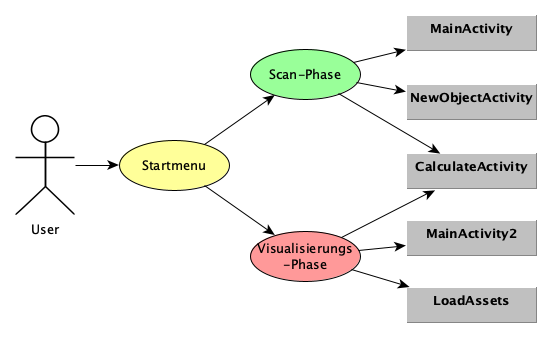
\includegraphics[width=13cm,height=13cm,keepaspectratio]{3Konzeption/Bilder/Anwendungsfalldiagramm.png}
    \caption{Anwendungsfall-Diagramm}
    \label{pic:anwendungsfall}
\end{figure}
\\ 
Nachdem auch das Softwarekonzept weitestgehend erarbeitet wurde, ging es um die Entscheidung, welches \acl{AR}-Framework für dieses Projekt 
ausgewählt wird. Nun wird die Evaluierung der Frameworks aufgegriffen, um einen Einblick in die Entscheidungsfindung zu gewähren.
\section{Auswahl des AR Frameworks}
\label{chap:Auswahl des AR Frameworks}
Mittlerweile gibt es eine enorme Auswahl an \acs{AR}-Frameworks, die alle unterschiedliche Präferenzen und 
Einsatzmöglichkeiten haben. Somit sind, auf den Bereich bezogen, Vor- und Nachteile im Vergleich von mehreren Frameworks nicht ausgeschlossen. 
Einige Alternativen wurden getestet und auf deren Brauchbarkeit evaluiert und analysiert. Dazu wurden Kriterien ausgearbeitet, die die 
Auswahl an Frameworks einschränken und nach Möglichkeit das passendste ergeben soll: 
\pagebreak
\begin{enumerate}
    \item Eine performante Darstellung von Objekten.
    \item Möglichkeiten zur Positionsbestimmung.
    \item Eine aktive Community und stetige Weiterentwicklung des Systems.
    \item Möglichkeit zur Integration weiterer Technologien.
    \item Open Source-Projekt, um Flexibilität und weitestgehende Unabhängigkeit zu gewährleisten.
\end{enumerate}
Aufgrund der großen Anzahl an \acs{AR}-Frameworks war es nicht möglich alle in Betracht gezogenen Frameworks detailliert aufzuführen. 
Lediglich die engere Auswahl der Tools wird aufgegriffen. 
\\ 
Nach ausführlicher Recherche wurden letzten Endes drei Frameworks in die nähere Auswahl aufgenommen, darunter \textit{vuforia}, 
\textit{ARToolKit} und \textit{Google ARCore}. Beweggründe zu dieser Entscheidung waren die überwiegende 
Übereinstimmung zu zuvor aufgestellten Kriterien und Anforderungen. Alle Technologien konnten eine aktive und große Community, sowie eine 
aktive Entwicklung, bzw. Weiterentwicklung vorweisen. Zusätzlich bieten alle Frameworks viele Möglichkeiten zur Integration weiterer 
Technologien, um nach Belieben immer mehr Funktionen in das zu entwickelnde System übernehmen zu können. Die Performance der Technologien konnte 
in allen Aspekten überzeugen und ist unter einfachen Bedingungen mehr als ausreichend. Ein Kritikpunkt gegen die Verwendung von vuforia war 
die fehlende Verfügbarkeit des Quellcodes, da dieser unter kostenpflichtiger Lizenz steht und nicht als Open Source-Projekt gilt. Das Framework 
vuforia wurde daher nicht in Betracht gezogen.
\subsection{ARToolKit}
ARToolKit ist ein \acs{SDK} zur plattformunabhängigen Entwicklung von \acl{AR} Anwendungen. Der Quellcode dieses Frameworks ist seit 2001 
frei verfügbar und ist vielseitig einsetzbar. Das Verfahren zur Positionsbestimmung durch Marker läuft schnell, problemlos und robust. Marker wie in 
Abbildung (\ref{pic:markerARpos}) werden schnell und ohne Probleme erkannt. Jedoch gibt es diesbezüglich Einschränkungen die beachtet werden 
müssen, um eine zuverlässige und stabile Markererkennung zu gewährleisten. Zu verhindernde Defizite sind Verdeckung des Markers, zu große Distanz 
von Kamera zu Marker, Blickwinkel auf den Marker und die Lichtverhältnisse des Umfelds. 
\\ 
Nachteilig dieses Frameworks für dieses Projekt ist die fehlende Unterstützung bei der Realisierung und Erkennung der Umgebung, bzw. des Umfelds.
So ist das Tracking nur über Marker, bzw. erweiterte markerbasierte Tracking-Methoden möglich. 
\\ %untauglich
Nach dieser Erkenntnis wurde auch dieses Framework als eher ungeeignet für die Verwendung in dem Projekt eingestuft. Möglicherweise 
gäbe es einen Weg, einen \acs{SLAM}-Algorithmus in Kombination mit ARToolKit unter erweitertem Aufwand zu verwenden, allerdings 
erschien dies zu umständlich und ineffektiv. 
\subsection{Google ARCore}
Google ARCore (siehe Abschnitt \ref{sec:arcore}) konnte bei der Analyse von sich überzeugen. Lediglich die Beschränkung der
Betriebssysteme auf \textit{Android} und \textit{iOS} ist ein kaum bedeutender Nachteil, da das Assistenzsystem in der Gesamtbetrachtung 
für ein Smart-Device konzipiert und entwickelt wird. Der entscheidende Vorteil bei 
ARCore ist der unterstützende Algorithmus zur Umgebungserkennung. Des Weiteren ist Google ARCore ein Open-Source Projekt und befindet sich 
in kontinuierlicher Weiterentwicklung. Neben der stetigen Entwicklung hat sich eine große und aktive Community gebildet, die bei auftauchenden 
Problemen zur Stelle ist. Ein weiterer Vorteil sind die verschiedensten Möglichkeiten der Interaktion mit \acs{AR}-Objekten. Es gibt die 
klassische Markererkennung, die nicht nur mit Markern (siehe Abbildung \ref{pic:markerARpos}) sondern auch mit Bildern funktioniert, dem sogenannten
\textit{AugmentedImage}. Darüber hinaus ist ARCore in der Lage Gesichter zu erkennen und diese als abgewandelte Marker zu verwenden, um eine konkrete 
Position ansprechen zu können. Diese Methode ist unter dem Namen \textit{AugmentedFace} bekannt. Eine weitere Methode ist die Erkennung von 
realen Punkten, Oberflächen und Gegenständen. So können virtuelle Objekte möglichst realitätsnah in den Raum visualisiert werden.
\\
\linebreak
Durch diese ganzen positiven Aspekte ist die Wahl des Frameworks auf das von Google entwickelte ARCore gefallen und wurde wegen den überzeugenden 
Grundlagen als Framework für dieses Projekt eingesetzt.

\section{Datenmodell}
\label{chap:Datenmodell}
Eine gute Basisstruktur der Datenspeicherung ist bei heutigem Datenverkehr sehr wichtig und hat hohe Priorität. Deshalb ist 
es sinnvoll, schon von Anfang an eine klare Richtlinie und Struktur zu erstellen, um bei nachträglichen Ergänzungen oder Änderungen zusätzlich so wenig 
Zeit wie möglich investieren zu müssen. Parallel zur Konzeption der Softwarearchitektur wurden Attribute zusammengetragen, die 
eine Basis von Informationen über verschiedenste Objekte aufgreifen soll. Mit den Objekten sind Gegenstände der realen Welt adressiert, die auch als 
virtuelle \acs{AR}-Objekte repräsentiert werden. 
\\
Bei der Datenmodellierung wurde entschieden, dass in der Scan-Phase (\ref{chap:Scan-Phase}), beim Erstellen eines Objekts, nur die notwendigsten 
Daten erhoben und gespeichert werden. Bei diesen Informationen handelt es sich um sogenannte Stammdaten. Bestandteile dieser Stammdaten sind Name, 
Größe und Baujahr des Objekts. Dazu kommen noch weitere relevante Informationen, darunter eine eindeutige ID zur genauen Erkennung eines Objekts und 
die virtuelle Position des \acs{AR}-Objekts. Die virtuelle Position ist durch die Scan-Phase gegeben und wird benötigt, um die Gegenstände in der 
Visualisierungs-Phase an der richtigen Stelle erneut einblenden zu können. 
\\ 
\linebreak 
Durch ein \acl{ERM} (\acs{ERM}) wurden die benötigten Daten zusammengetragen, aufgeführt und zu einem Modell konzipiert, um den Strukturen und 
Vorgaben der Datenmodellierung zu entsprechen und eine gute Basisstruktur zu erschaffen. Mit dieser Grundlage kann in Zukunft weitergearbeitet werden. 
Das Modell wurde mit der zuvor angesprochenen dritten Normalform umgesetzt, da diese die perfekte Balance in dem Datenmodell herstellt, um auftretende 
Probleme möglichst einfach zu lösen und diese nahe der Realität in das relationale Datenbankmodell einzupflegen. Dadurch kann eine Erweiterung des 
Datenmodells gewährleistet werden. Die Abbildung (\ref{pic:erm}) zeigt das erstellte ER-Modell auf und veranschaulicht die Modellierung. 
\\ 
\pagebreak
\begin{figure}[hbt!]
    \centering
    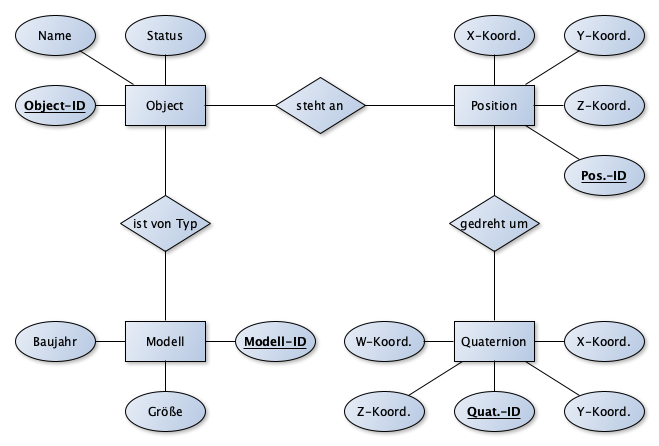
\includegraphics[width=15cm,height=15cm,keepaspectratio]{3Konzeption/Bilder/ERM_BA.png}
    \caption{Entity Relationship Datenmodell}
    \label{pic:erm}
\end{figure}
\\
Nach Beendigung des Datenkonzepts waren alle notwendigen Konzeptionen abgeschlossen. Diese wurden in Summe zusammengetragen, im Gesamten nochmals 
betrachtet und anhand neu gewonnener Kenntnisse überarbeitet und evaluiert. Da zu diesem Zeitpunkt alle Konzeptionen abgeschlossen 
waren, konnten diese zusammen analysiert und überdacht werden. 
\\ 
\linebreak
Nachdem die Phase der Konzeption endgültig abgeschlossen war, konnte die Umsetzung des Konzepts und die Entwicklung des Systems starten. 
% 
%%%%%%%%%%%%%%%%%%%%%%%%%%%%%%%%%%%%%%%%%%%%%%%%%%%%%%%%%%%%%%%%%%%%%%%%%%%%%
%% Descr:       Vorlage für Berichte der DHBW-Karlsruhe, Ein Kapitel
%% Author:      Prof. Dr. Jürgen Vollmer, vollmer@dhbw-karlsruhe.de
%% $Id: kapitel2.tex,v 1.5 2017/10/06 14:02:51 vollmer Exp $
%%  -*- coding: utf-8 -*-
%%%%%%%%%%%%%%%%%%%%%%%%%%%%%%%%%%%%%%%%%%%%%%%%%%%%%%%%%%%%%%%%%%%%%%%%%%%%%%%

\chapter{Umsetzung}
\label{chap:Umsetzung}
Dieses Kapitel greift die in der Konzeption (\ref{chap:Konzeption}) aufgeführten Planungen und Ideen auf und legt die Implementierung, bzw. 
Umsetzung detaillierte dar. Darunter sind Lösungsansätze aufgezeigt und aufgetretene Probleme und deren Behebung dokumentiert. Allgemein zählt 
dazu die Umsetzung des Startmenüs und der beiden Kernfunktionen. Sowohl die Frontend- als auch die Backend-Aspekte werden in der Implementierung 
(\ref{chap:implementierung}) aufgezeigt. 

\section{Implementierung}
\label{chap:implementierung}
Nachdem die Konzeption endgültig abgeschlossen war, ging es an die Umsetzung des Konzepts und an die Implementierung der Funktionen, die das System 
ausmachen. 
\\ 
Die Use Cases und deren Implementierung wurden nach logischer und chronologischer Reihenfolge entwickelt und dokumentiert. Diese festgelegte Reihenfolge 
ist auch der Abbildung (\ref{pic:anwendungsfall}) zu entnehmen. Angefangen mit dem Startmenü, das dem Nutzer die Möglichkeit offenbart, zwischen den Funktionen 
zu wählen, folgte die Implementierung der Scan-Phase, in der die realen Objekte virtualisiert und im Raum platziert werden. Zu guter Letzt kam die Visualisierungs-Phase, 
welche aufbauend auf die Scan-Phase funktioniert und die zuvor gescannten Objekte erneut virtuell im Raum einsetzt. 
\\ 
Beim ersten Gebrauch der Anwendung ist eine vorzeitige Nutzung der Visualisierungs-Phase ohne weiteres nicht möglich. Zuvor muss der Nutzer einen Scan durchführen, sodass 
das System Daten generiert, Informationen liefert und diese zur Verfügung stellt. Dies hat zur Folge, dass die zweite Kernfunktion mit den zuvor erzeugten Informationen 
durch die Scan-Phase operiert und ausgeführt werden kann. 
\\ 
\linebreak 
Aufgeteilt wurden die Use Cases der Anwendung jeweils immer nach Frontend und Backend, demnach wird auch die Dokumentation in diesem Stil geschildert. 
\\ 
\linebreak
Bevor die Umsetzung verwirklicht werden konnte, wurden vorab noch die letzten Vorbereitungen durchgeführt.
\\ 
Zum Start der eigentlichen Implementierung war es die Aufgabe, die Entwicklungsumgebung zu wählen und einzurichten, um bestmöglich arbeiten zu können. Als 
\ac{IDE} wurde die speziell für Android-Applikationen entwickelte Software \textit{Android Studio} ausgesucht. Diese ist besonders für die Entwicklung von 
Android-Applikation geeignet, ausschließlich für Hardware, dessen Software das Android Betriebssystem nutzt. 
\\
Android Studio ist von Google LLC. und JetBrains entwickelt und basiert auf der IntelliJ IDEA Community Edition \acs{IDE}. Als 
Build-Management-Automatisierungs-Tool stellt Android Studio das Tool Gradle zur Verfügung, welches die zu bauenden Projekte durch die verwendeten 
Dependencies, Frameworks und Tools beschreibt. Um die notwendigen Libraries in der Applikation verwenden zu können, werden in dieser Datei unter 
anderem die Bibliotheken und deren verwendete Version eingetragen. Im Fall des zu entwickelnden Unterstützungssystems wurden dort die Bibliotheken zur 
Nutzung der Android Architecture Components eingetragen, darunter Room und LiveData. 
Darüber hinaus wird dort auch die Version des ARCore Frameworks und des Sceneform \acs{SDK}s verwaltet, welches ebenso essentielle Bestandteile der 
Applikation sind.
\\ 
Nachdem alle Abhängigkeiten erfolgreich eingebunden waren, wurden zur übersichtlichen Gestaltung der Klassen, Objekte, ViewModel, Repositories und Activities 
eine Ordnerstruktur angelegt, die alle Klassen des gleichen Typs im Laufe der Entwicklung beinhalten sollten. Dadurch kann bei der Programmierung besser und 
übersichtlicher durch das Projekt navigiert werden und  es befinden sich alle Klassen ähnlicher Eigenschaften im selben Zielordner. 
\\ 
\linebreak
Damit im Laufe der Entwicklung die Applikation bestmöglich getestet werden konnte, war es notwendig, ein Testgerät zu verwenden. Mit dem verfügbaren 
Emulator\footnote{Ein System, das ein anderes in speziellen Teilbereichen nachbildet} von Android Studio konnte keine realitätsnahe Testung 
durchgeführt werden. Deshalb wurde zum Testen der Anwendung ein Smartphone benutzt. Dieses musste zu Anfang unter den vorbereitenden Maßnahmen des 
Projekts organisiert werden.
\\ 
\linebreak
Nachdem nun alle Schritte abgeschlossen waren, ging es an die Entwicklung des ersten Use Cases, dem Startmenü, um die Grundlage des Systems zu festigen.  

\subsection{Startmenü}
Das Startmenü ist die zentrale Anlaufstelle des prototypischen Unterstützungssystems und bildet den Einstiegspunkt in die Interaktionen zwischen Anwender 
und der Applikation, dem Assistenzsystem.
\\ 
Nun folgt die Beschreibung der Implementierung des Startmenüs, sowohl des Frontends als auch des Backends.

\subsubsection{Frontend}
Wird das Unterstützungssystem heruntergeladen, genauer gesagt auf die verwendete Hardware geladen, folgt das Speichern der Anwendung auf dem Gerät. Die Applikation 
erscheint auf dem Applikationshauptmenü des Smart-Devices und wird dort zur Nutzung zur Verfügung gestellt. 
\\ 
Beim Start öffnet sich das Hauptfenster der Applikation und darin das Startmenü, auf das im Verlauf noch genauer eingegangen wird. 
\\ 
Zuallererst werden bei initialer Instandsetzung bestimmte Genehmigungen eingeholt, um die Anwendung überhaupt starten zu können. Darunter soll der Nutzer dem System 
die Erlaubnis erteilen, auf die Kamera zugreifen zu dürfen. Um die Umgebung in der Hauptfunktion scannen zu können, muss diese in weiterer Abfolge des Assistenzsystems genutzt werden können. 
Diese Abfrage erfolgt über ein kleines PopUp-Fenster, welches von Android fest vorgegeben ist. Dieses Fenster ist der Abbildung (\ref{pic:camera_perm}) 
zu entnehmen. Mit dem Zulassen des Zugriffs auf die Kamera kann der Nutzer und die Applikation wie gewünscht fortfahren. Wird allerdings der Zugriff abgelehnt, kann 
die Applikation nicht starten, bzw. wird der Zugriff auf die Kamera verweigert, kann die Applikation nicht einwandfrei benutzt werden.     
\begin{figure}[hbt!]
    \centering
    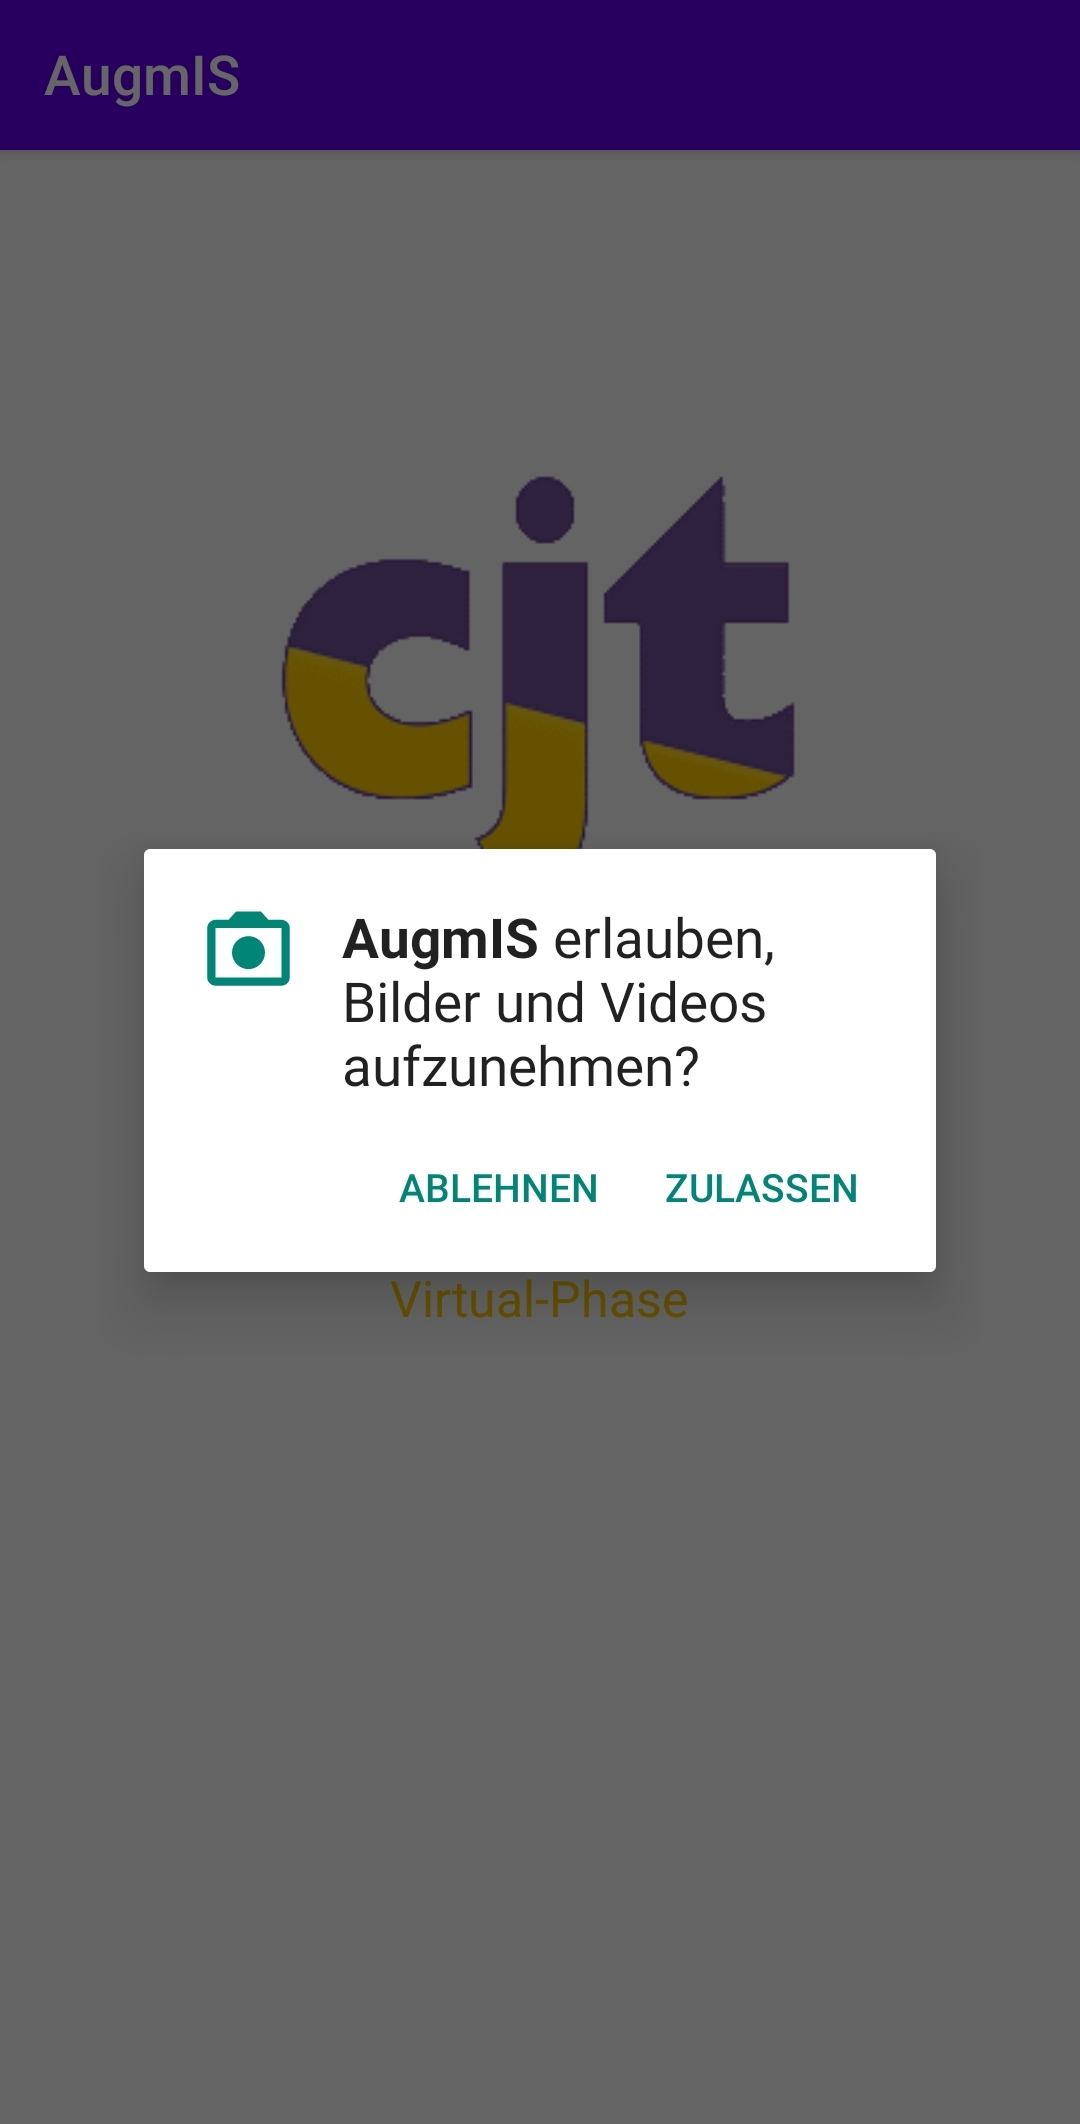
\includegraphics[width=10cm,height=7.5cm,keepaspectratio]{4Umsetzung/Bilder/camera_permission.jpg}
    \caption{Start der Applikation}
    \label{pic:camera_perm}
\end{figure}
\\ 
\linebreak
Da speziell das Assistenzsystem auf die gegebenen Komponenten der Hardware zugreift, z. B. die im Smart-Device integrierte Kamera, zählt diese zu den nativen Applikationen. 
Darunter sind Anwendungen zu verstehen, die ausdrücklich für das Betriebssystem des Endgeräts konzipiert sind oder die zum Beispiel auf die vom Endgerät vorhandenen 
Komponenten zugreifen, wie in etwa auf die Bild-Mediathek, der Datei-Strukturen oder die oben bereits erwähnte Kamera-Komponente.
\\ 
\linebreak
Angenommen der Nutzer lässt den Zugriff auf die Kamera für das Assistenzsystem zu, dann startet die Applikation wie erwünscht. Darauffolgend ist dann 
das eigentliche Startmenü zu sehen. Diese Ansicht ist der nachfolgenden Abbildung (\ref{pic:startmenu}) zu entnehmen. Die Benutzeroberfläche weist ein sehr einfaches und 
schlicht gehaltenes Design auf. 
Darauf ist das Firmen-Logo der cjt Systemsoftware AG zentriert zu sehen, außerdem zwei farblich voneinander getrennten Buttons zur Navigation innerhalb der Applikation. 
Die Buttons adressieren jeweils die nachfolgende, zugehörige Funktion. Dies sind zum einen der lilafarbenen Button, der zur Scan-Phase weiterleitet und zum anderen der 
gelbfarbene Button, der den Nutzer zur Visualisierungs-Phase navigiert. In der Gesamtheit ist das Layout an den Farben des Firmen-Logos angelehnt und bildet einen 
ruhigen und harmonischen Einstieg in das Programm. 
\\ 
\linebreak
Grundlegend wurden für die Designs der Benutzeroberflächen Prinzipien der \ac{UX}, berücksichtigt. Darunter folgende Punkte: 
\pagebreak
\begin{itemize}
    \item Übersichtlichkeit (Digestibility): Auf einen Blick verstehen, worum es geht. Der User versteht intuitiv was zu tun ist.
    \item Klarheit (Clarity): Deutliche und verständliche Ausdrucksweise und klar herauszufindenden Nutzen der Funktion, bzw. Anwendung.
    \item Vertrauen (Trust): Gutes Design erlangt Vertrauen. Offenlegung der Aktionen und Hintergründe. 
    \item Begeisterung (Delight): Komplexe Sachverhalte einfach zu lösen. 
\end{itemize} 
\begin{figure}[hbt!]
    \centering
    
\includegraphics[width=10cm,height=7.5cm,keepaspectratio]{4Umsetzung/Bilder/startmenu.jpg}
    \caption{Startmenü der Applikation}
    \label{pic:startmenu}
\end{figure}
Nachdem das Design des Startmenüs und dem PopUp-Fenster abgeschlossen war, ging es darum, die Funktionalität der UI-Komponenten zu implementieren. 
\subsubsection{Backend}
Durch die schlichte und einfach gehaltene Modellierung des Startmenüs, zählt dieses als Ansicht zum Einstieg in die Nutzung des Assistenzsystems, zur Abfrage der 
\textit{„Camera-Permission“} und zur weiteren Navigation innerhalb der Anwendung.
\\ 
Mit der \textit{„Permission-Request“} wird abgefragt, ob die Genehmigung zur Nutzung der Kamera in der \textit{„AndroidManifest.xml“}-Datei erteilt wurde, bzw. 
dadurch wird das PopUp-Fenster zur Nachfrage der Genehmigung geöffnet und die daraus resultierende Antwort in die Manifest-Datei eingetragen. 
\\ 
\linebreak
Die Manifest-Datei beinhaltet alle optionalen Metadaten, die für das Assistenzsystem benötigt werden. Dazu gehören die Google ARCore-Metadaten, sowie 
grundlegende Informationen über das Projekt, die das Android-System erfordert, um die Applikation installieren und ausführen zu können. Dazu wird unter 
anderem die Berechtigung zur Kameranutzung benötigt, ebenso werden Angaben zu Activities, bzw. Benutzeroberflächen gemacht und Stammdaten, z.B. Titel, -bild und 
App-Icon, die das Projekt eindeutig spezifizieren, definiert.
\\ 
\linebreak
Demnach beinhaltet die Backend-Funktion des Startmenüs die Abfrage der \textit{„Camera-Permission“} und die Button-Klick-Funktionen, die den Nutzer 
jeweils auf die von ihm gewählte Funktion weiterleiten. Sozusagen handelt es sich um eine simple Navigation.
\\ 
\linebreak
Als das Startmenü implementiert war, ging es an die Entwicklung der Scan-Phase, der ersten Kernfunktion des Assistenzsystems.

\subsection{Scan-Phase} %Umgebungserkennung /
\label{chap:scan_implementation}
Bei der Implementierung der Scan-Phase kam es zu den ersten praktischen Berührpunkten mit der Google ARCore \acs{API}. Diese wurde zu Beginn studiert, 
um einen Überblick, wie die Struktur dieser Schnittstelle aufgebaut ist, zu erlangen. Dadurch konnten Methoden und Funktionen analysiert werden, um im 
weiteren Verlauf der Entwicklung damit arbeiten zu können.
\\ 
Die Idee hinter der Scan-Phase ist die Implementierung einer Methode, die es ermöglicht, das Umfeld über die Kamera wahrzunehmen und mit den gewonnenen 
Erkenntnissen über den Raum weiterarbeiten zu können. Die nachstehende Funktion, virtuelle Objekte auf Basis der vom Scan erfahrenen Kenntnissen in 
der Räumlichkeit zu platzieren, arbeitet mit diesen in Erfahrung gebrachten Kenntnisse. 
\\ 
Zur Schaffung einer Grundlage, um die wichtigsten Funktionen zu implementieren, wurden zuallererst die Benutzeroberflächen erstellt. Diese dienen 
unter anderem dazu, den Fokus für die Funktionsweise der eigentlichen Methode nicht zu verlieren. Demnach werden die entwickelten \acs{GUI}s nun aufgeführt 
und näher beschrieben, um Methoden des Backends im Anschluss besser nachvollziehen zu können.
\subsubsection{Frontend}
Das Assistenzsystem verfügt über eine Vollbildkamera-Ansicht, die mit einem weißen Rahmen überlagert ist. Damit können über die Kamera Bilder zentriert 
eingefangen werden. Somit weiß der Nutzer, wie er das Smart-Device in Position bringen muss, damit er das zu scannende Bild über die Kamera 
bestmöglich erfassen kann. 
\\ 
\linebreak
Ursprünglich war die Applikation nicht mit diesem Layout (\ref{pic:image_tracking}) konzipiert, da während der Implementierung der Scan-Phase eine 
schwerwiegende Änderung vorgenommen werden musste. Diese wird in dem Abschnitt der Scan-Phasen-Backend-Entwicklung zu gegebenem Zeitpunkt 
aufgegriffen und genauestens dargelegt. 
\begin{figure}[hbt!]
    \centering
    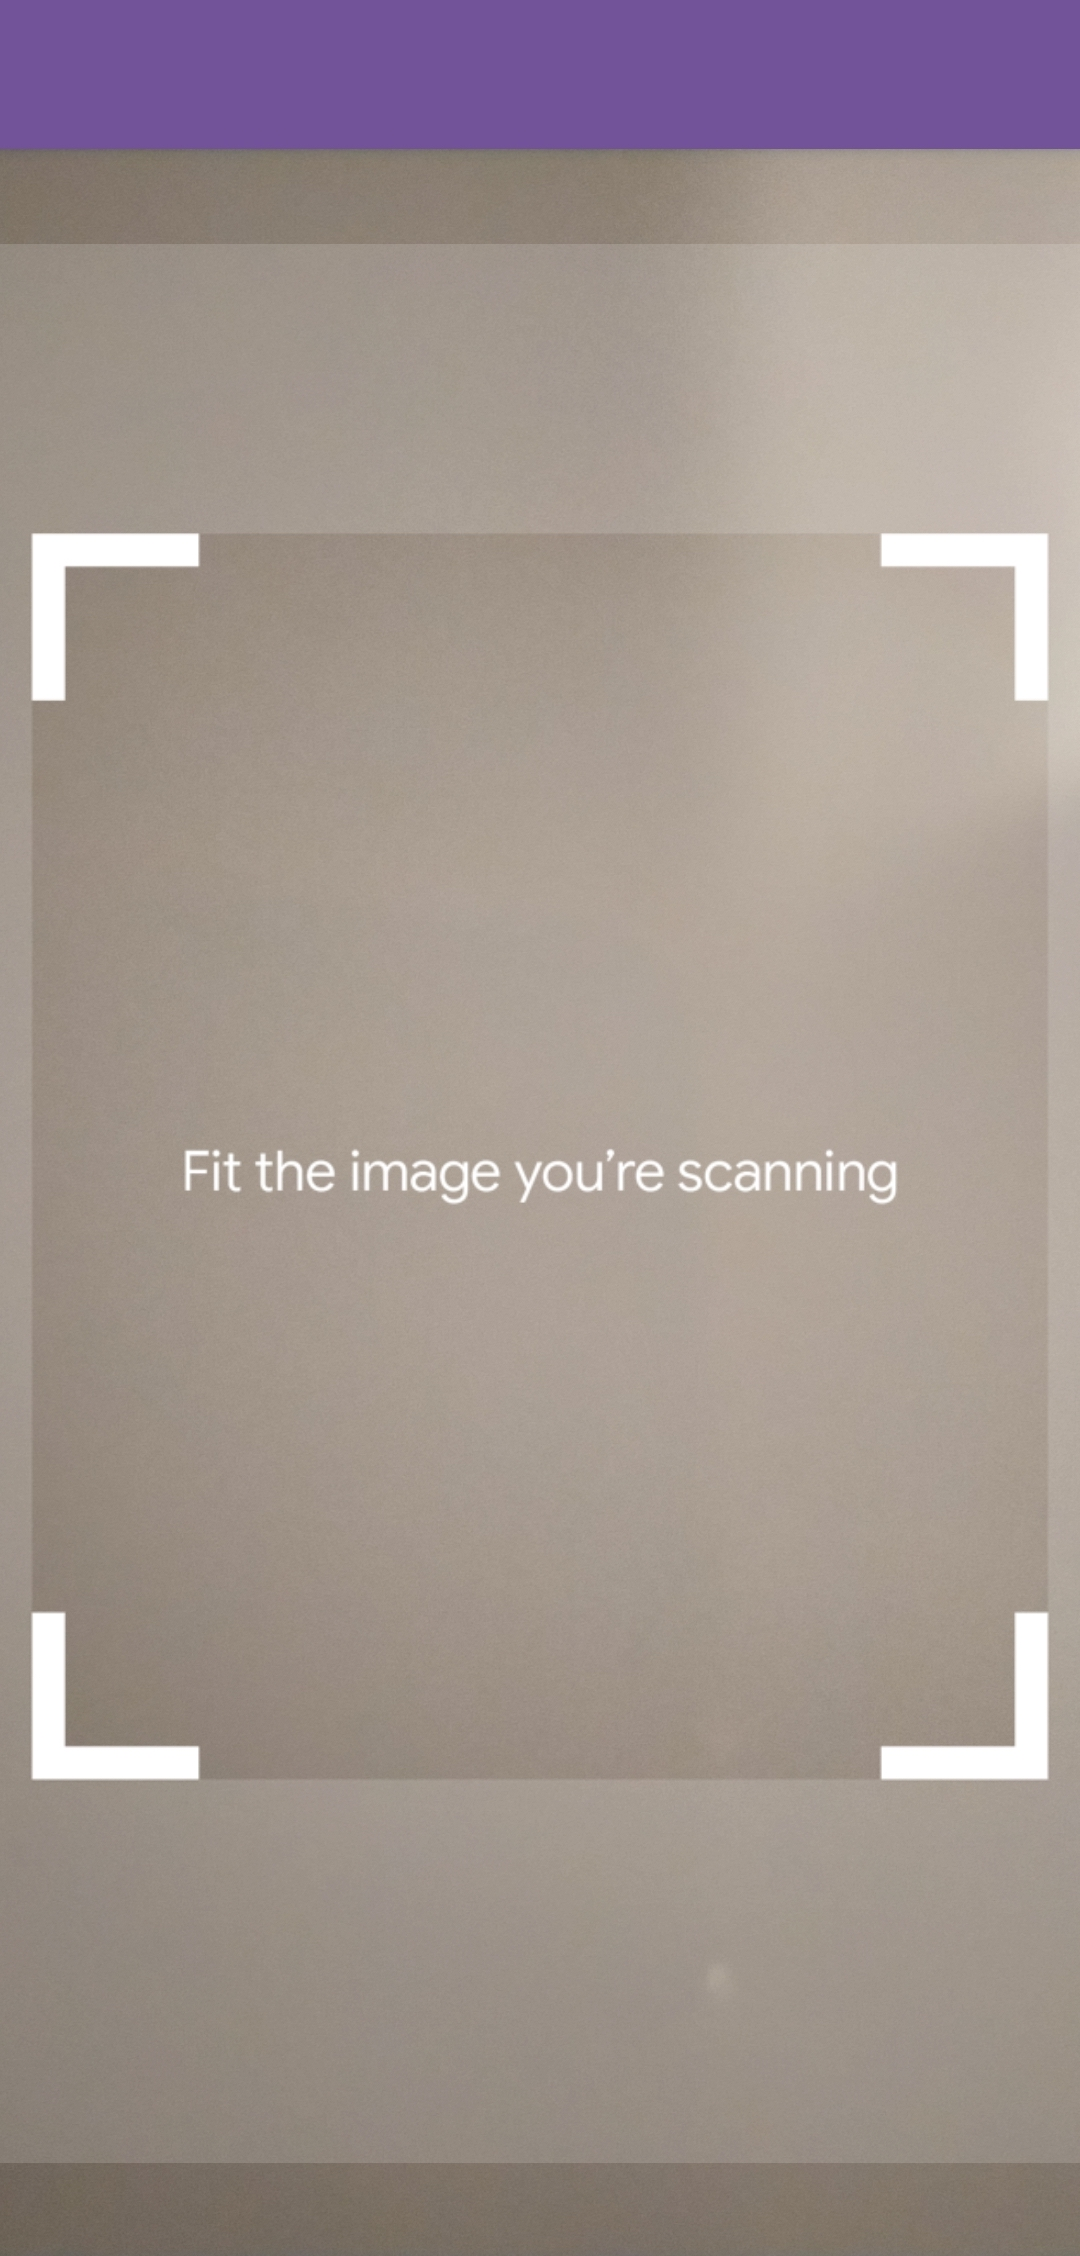
\includegraphics[width=10cm,height=7.5cm,keepaspectratio]{4Umsetzung/Bilder/image_tracking.jpg}
    \caption{Markererkennung der Applikation zum Start der Scan-Phase}
    \label{pic:image_tracking}
\end{figure}
\pagebreak 
\\
\linebreak 
Des Weiteren beinhaltet das Assistenzsystem die eigentliche Scan-Phasen \acs{UI}, mit der die Umgebung aufgenommen wird und anhand dieser Daten 
der Nutzer die Objekte an von ihm definierte Stellen platzieren kann. Die Benutzeroberfläche hat ebenso ein schlichtes und überschaubares Layout, 
welches dem Anwender zugutekommt. 
\\ 
Hauptsächlich beinhaltet die \acs{GUI} ein Fragment, welches das Kamerabild in Echtzeit wiedergibt. Am oberen Ende des Bildschirms, bzw. der Abbildung 
(\ref{pic:scan}) befindet sich eine lilafarbene Fläche, die zur Anzeige von Informationen vorhanden ist und gleichzeitig als erweiterte Abgrenzung 
zur Topdown-Leiste dient. Am unteren Ende des Bildes befindet sich eine \textit{„Android-Gallery“}, die alle zu platzierenden Objekte beinhaltet. In 
der zugrundeliegenden Abbildung sind es zwei Platzhalter-Objekte, die bei Berührung des Bildes erstellt werden. Prinzipiell ist diese Gallery um 
beliebig viele Objekte erweiterbar. Diese Erweiterung erfolgt allerdings nicht dynamisch, sondern muss über manuelles Einfügen im Code stattfinden. 
\\
Wird während der laufenden Anwendung ein Objekt über dessen Button erstellt, wird der Nutzer unverzüglich auf eine weitere Seite (\ref{pic:createObject}) 
geleitet, um parallel zur Renderung des Objekts Informationen diesbezüglich der Datenbank hinzufügen zu können. Auf dieses Layout wird im weiteren Verlauf der 
Ausarbeitung noch eingegangen. Vorwegzunehmen ist, dass die Informationen mit den Daten der virtuellen Position in der Datenbank persistiert werden.
\\ 
\linebreak 
%Damit der Scan-Vorgang gestartet wird
Bevor der Scan-Vorgang startet, wird inmitten des Fragments ein Overlay angezeigt, welches eine Geste, bzw. Bewegung vorgibt. Imitiert der Nutzer 
diese Bewegung, wird der Scan-Prozess anlaufen.
\\ 
\linebreak
Um weiterhin auf der Seite navigieren zu können, gibt es im rechten unteren Eck einen weiteren Button, welcher ebenso der Abbildung (\ref{pic:scan}) 
zu entnehmen ist. Diese Schaltfläche leitet den Nutzer weiter, bzw. wieder zurück zum Startmenü und beendet die Scan-Phase. 
\\ 
\linebreak
Damit der Nutzer über die in der Datenbank gespeicherten Informationen mehr Möglichkeiten besitzt, gibt es im linken oberen Eck der \acs{UI} eine zusätzliche 
Schaltfläche versehen mit einem roten Kreuz versehen. Dadurch hat der Nutzer die Möglichkeit, alle vorhandenen, in der Datenbank persistierten Informationen zu 
löschen und den Scan-Vorgang erneut von der ursprünglichen Ausgangsposition zu beginnen. Nachdem die Daten gelöscht werden, wird der Nutzer aufgefordert, den 
Ursprungspunkt, den zu \textit{„trackenden“} Marker, abzuscannen und die Phase erneut zu beginnen. 
\\ 
Mit dieser Funktion verfügt der Nutzer über mehr Entscheidungsmöglichkeiten, bevor die Applikation komplett gelöscht und neu aufgespielt werden muss.
\begin{figure}[hbt!]
    \centering
    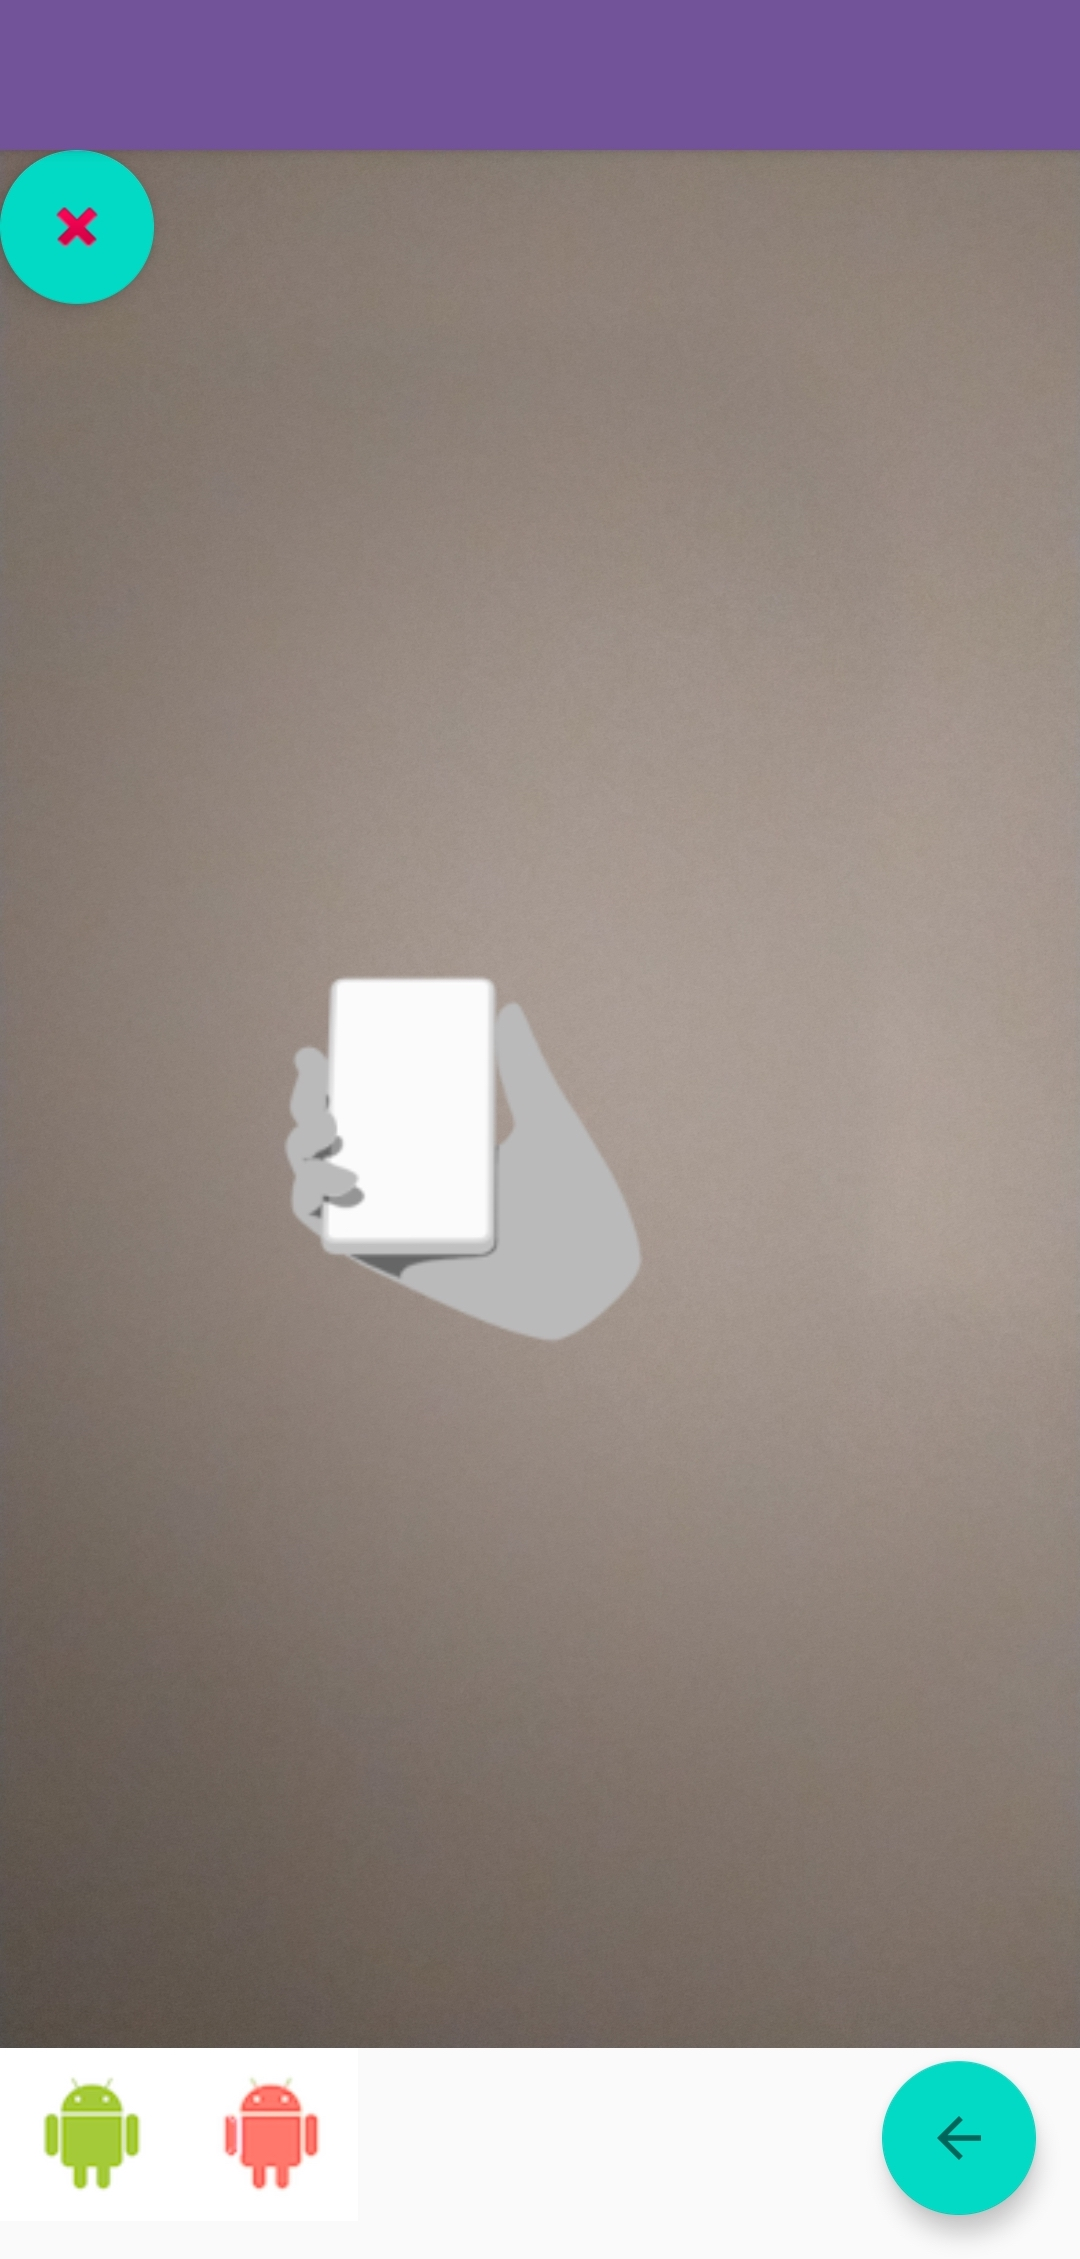
\includegraphics[width=10cm,height=7.5cm,keepaspectratio]{4Umsetzung/Bilder/scan-phase.jpg}
    \caption{Scan-Phase der Applikation}
    \label{pic:scan}
\end{figure}
\\ 
\linebreak
Zu dem Zeitpunkt, wenn der Anwender ein Objekt erstellen und zusätzliche Informationen hinzufügen möchte, wird darauffolgend eine weitere \acs{UI} 
angezeigt. Bei dieser Ansicht ist vorgesehen, dass der Nutzer die zu dem erstellen Objekt dazugehörigen Informationen einträgt, sodass diese anschließend 
in die Datenbank aufgenommen werden können. Die Benutzeroberfläche verfügt über mehrere Text-Eingabefelder, die ein Großteil der Daten des Datenmodells 
abdecken. In Abbildung (\ref{pic:createObject}) sind diese Felder zusehen. Dabei werden Informationen über den Objektnamen, -baujahr, -größe, sowie 
-status von der Person, die das Assistenzsystem nutzt, gefordert. 
\\ 
Im Hintergrund werden ebenso die Daten der Position und Drehung des 
Objekts bereitgestellt. Die wird im Backend näher erläutert. Über die Betätigung des \textit{„save“}-Buttons werden die Informationen lokal gespeichert und für die Eintragung in die Datenbank 
vorgemerkt. Nachdem der Button bedient wurde, wird der Anwender auf die Oberfläche der Scan-Phase weitergeleitet, um bei Bedarf weitere Objekte zu 
erstellen.  
\begin{figure}[hbt!]
    \centering
    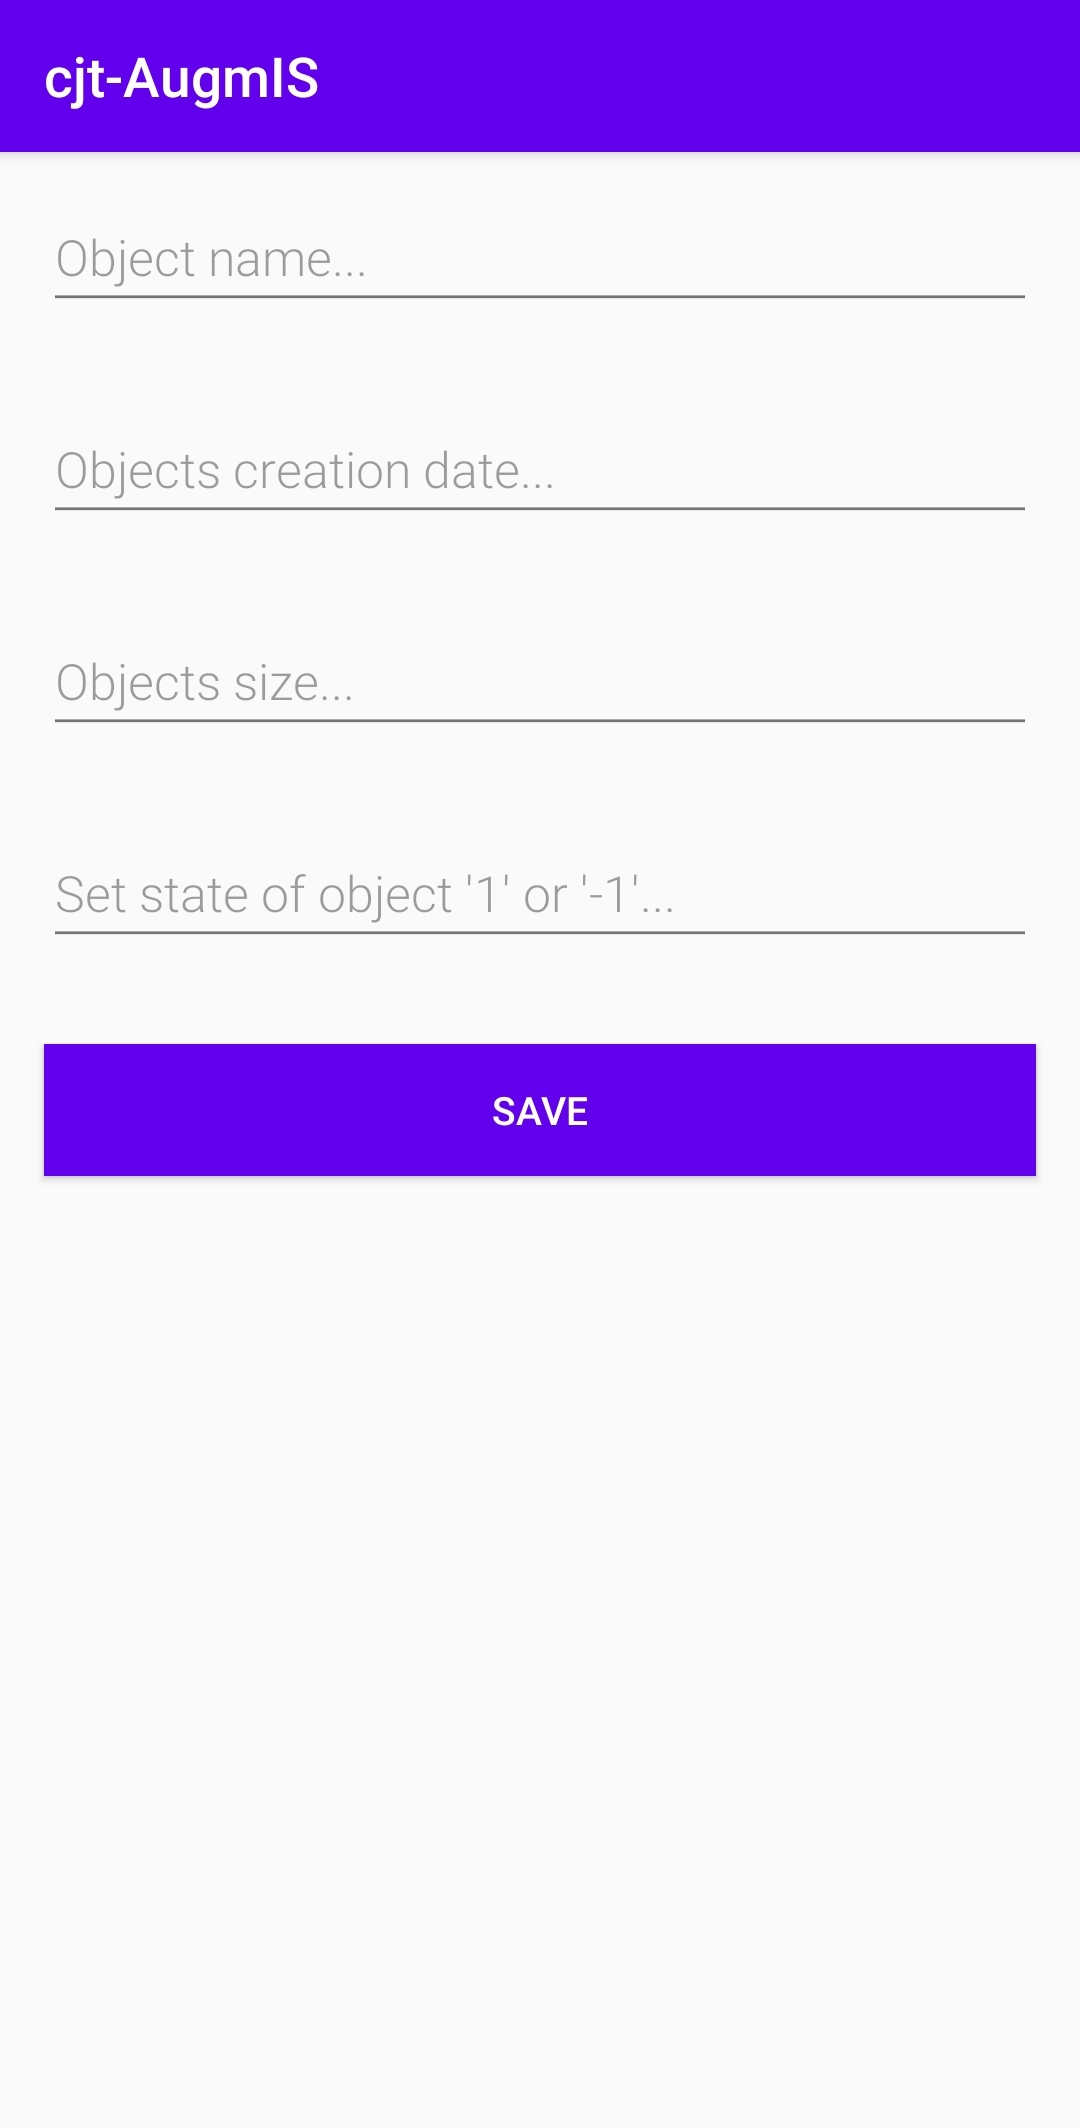
\includegraphics[width=10cm,height=7.5cm,keepaspectratio]{4Umsetzung/Bilder/objekt_info.jpg}
    \caption{Erstellen eines neuen Objekts}
    \label{pic:createObject}
\end{figure}
\pagebreak
\\ 
%\linebreak
Nachdem der Abschnitt der Frontend-Entwicklung vollends dargelegt wurde, geht es mit den Funktionen im Backend weiter. Darüber hinaus werden in diesem 
Abschnitt auch die Lösungsansätze, sowie aufgetretene Probleme und deren Behebung genauestens aufgeführt und geschildert, damit der Nutzer mit der 
aufgetretenen Problematik vertraut wird und die Entscheidungen und Lösungsfindungen nachvollziehen kann. 
% \subsubsection{Backend}
Mit Beginn der Backend-Entwicklung wurden in erster Linie die Grundstrukturen implementiert, um der \textit{MVVM}-Architektur gerecht zu werden. Dabei lag 
der Fokus bei der Instanziierung der notwendigen Komponenten der \textit{Android Architecture Components}. Nach chronologischer Reihenfolge wurden die Klassen 
erstellt und mit den dazugehörigen Funktionen und Methoden versehen. Angefangen mit der Entity-Klasse zur Beschreibung des Objekts und deren allgemeinem Aufbau, 
der bereits in der Konzeption (\ref{chap:Konzeption}) unter dem Datenmodell (\ref{chap:Datenmodell}) festgehalten wurde. Darauffolgend wurde das „Data Object“ 
erstellt, welches die Zugriffe der Datenbankobjekte verwaltet. Abschließend wird im Bereich der Datenbank ein Room-Layer eingebaut, um die eigentliche Datenbank zu 
instanziieren und eine Zugriffsschicht auf diese zu implementieren. 
\\ 
Zur Modularisierung und Generierung einer Schnittstelle zur Kommunikation zwischen einzelnen Datenbeziehungspunkten und der Datenbank wurde ein Repository erstellt, 
das aus verschiedenen Quellen Daten zusammenbringen kann und eine saubere \acs{API} für den Datenzugriff auf den Rest der Anwendung bietet. 
Um die vorhandenen Klassen zum Datentransfer und zum Persistieren der Daten mit der 
eigentlichen Benutzeroberfläche zu verbinden, wurde ein ViewModel implementiert, welches die Daten zwischen den einzelnen Komponenten teilt und bereitstellt. 
\\ 
\linebreak 
Nach Aufzählung der einzelnen Bestandteile wird auf diese nun genauer eingegangen. 
\\ 
\linebreak
In einer Java-Klasse wird mithilfe der gegebenen Bibliothek „Room“ ein Entity-Objekt erstellt. Hierbei gibt es eine eindeutige Annotation, die die Klasse und 
deren beinhalteten Variablen deklariert. In dem folgend aufgeführten Code-Beispiel (\ref{code:entity}) ist diese Annotation zu entnehmen, in dem eine Klasse als 
Entity deklariert und somit in eine Datenbank-Tabelle konvertiert wird. 
In dieser Tabelle, definiert als \textit{„object\_table“}, gibt es weitere Variablen, die zuerst mit Annotationen versehen und dann gemäß der Anforderungen des 
Konzepts sind. Diese Variablen repräsentieren die Attribute des Datenbankschemas und stellen die einzelnen 
Informations-, bzw. Datenbankspalten dar. Zur Veranschaulichung dient die Initialisierung der \acs{ID}-Vergabe eines Objekts. Diese wird als \textit{„id“}-Spalte 
und ebenso als Primärschlüssel\footnote{Einmaliger und eindeutiger Wert einer Tabelle, bzw. eines Attributs, um dieses eindeutig zu kennzeichnen.}-Variable 
deklariert.
\\ 
\linebreak
\begin{lstlisting}[language=C,
    frame=lines,           % Ein Rahmen um den Code (single for box, lines for top and bottom)
    xleftmargin=\parindent,  % Rahmen link von den Zahlen
    style=algoBericht,
    label={code:entity},
    captionpos=b,           % Caption unter den Code setzen
caption={Entity Code zur Initialisierung der Objekte}]
@Entity(tableName = "object_table")
public class Object {
    @ColumnInfo(name = "id")
    @NonNull
    @PrimaryKey(autoGenerate = true)
    private int id;

    public int getId() { return this.id; }
    public void setId(int id) { this.id = id; }
    ... 
}
\end{lstlisting}
\pagebreak
Das mit der Entity-Klasse kommunizierende Modul ist das \textit{„Data Object“}, welches als Interface angelegt wurde. Das „Object Dao“ verwendet ebenso die Bibliothek 
„Room“ und wandelt die Java-Klasse per Annotation in ein „Dao“ um. Dieses beinhaltet hauptsächlich die SQL-Queries zur Datenabfrage der vorhandenen Informationen. 
\\
\linebreak
\begin{lstlisting}[language=C,
    frame=lines,           % Ein Rahmen um den Code (single for box, lines for top and bottom)
    xleftmargin=\parindent,  % Rahmen link von den Zahlen
    style=algoBericht,
    label={code:query},
    captionpos=b,           % Caption unter den Code setzen
caption={SQL-Query zur Abfrage der Objekt-Namen}]
@Query("SELECT * FROM object_table ORDER BY name")
LiveData<List<Object>> getObjectName();
\end{lstlisting}
Nachdem die beiden Klassen erstellt worden sind, wurde das Datenbank-Layer auf der eigentlichen Datenbank implementiert. Über einen „Builder“ wird die 
Datenbank-Instanz erzeugt und mit einem Namen versehen. Im Falle des Assistenzsystems als \textit{„object\_database“} deklariert. 
\\ 
In zukünftigen Entwicklungen, 
falls notwendig, gäbe es die Möglichkeit, in diesem Schema weitere Datenbanken zu erstellen und diese über weitere „Dao“s zu referenzieren. Darüber hinaus ist die 
Möglichkeit gegeben, weitere Datenbank-Tabellen zur Speicherung von Objekten und deren Informationen zu erstellen. Ebenso ist durch ein Repository die Option 
geboten, die derzeit auf dem Smartphone gespeicherte Datenbank auf einen externen Server auszulagern, um so die Daten weitläufiger zur Verfügung zu stellen. 
Eine Datenbeziehung von generierten Daten der Maschinen und Geräten selbst wäre auch vorstellbar, allerdings müssten diese vorab noch aufbereitet 
und zur Nutzung bereitgestellt werden. Diese Methode wird allerdings nicht näher betrachtet, da sie nicht Teil dieser Arbeit ist. 
\\ 
Im Ausblick (\ref{chap:Ausblick}) wird darauf nochmals eingegangen.
\\ 
\linebreak
\begin{lstlisting}[language=C,
    frame=lines,           % Ein Rahmen um den Code (single for box, lines for top and bottom)
    xleftmargin=\parindent,  % Rahmen link von den Zahlen
    style=algoBericht,
    label={code:dblayer},
    captionpos=b,           % Caption unter den Code setzen
caption={Erzeugung des Datenbank-Layers „Room“}]
@Database(entities = {Object.class}, version = 1, exportSchema = false)
public abstract class ObjectRoomDatabase extends RoomDatabase {
    ...
    INSTANCE = Room.databaseBuilder(context.getApplicationContext(),
    ObjectRoomDatabase.class, "object_database")
    .addCallback(sRoomDatabaseCallback)
    .build();
    ...
}
\end{lstlisting}
Letzter wichtiger zu implementierender Aspekt war das Kommunikations-Modul zwischen den Datenbank-Transferen und der Benutzeroberfläche, das ViewModel. 
In dieser Klasse wird beim Start der Anwendung eine Liste anhand der Objekte in der Datenbank erstellt, welche die Informationen des einzelnen Objekts besitzt. 
Diese werden über eine „get“-Funktion aus dem zuvor instanziierten Repository geladen und in der erzeugten Liste lokal abgelegt. Diese Liste wird dann für 
die Präsentation der Informationen auf der Nutzeroberfläche verwendet. Bei Änderungen der Informationen wird über die \acs{UI} der „Oberserver“ benachrichtigt. 
Dieser registriert die Änderungen und überträgt sie nach vollständigem Abschluss der Transaktion in die Datenbank. Der Transfer erfolgt wiederum über das 
Repository, da dort die Datenbankzugriffe verwaltet und aufgerufen werden. %%%%%%%---------->> Genauer ausführen, wie das funktioniert!!!!!!!
\\ 
\linebreak
Die ursprünglich anders angedachte Implementierung der eigentlichen Scan-Phase unter Beachtung der ARCore-\acs{API} stellte sich im Laufe der Entwicklung 
als nicht praktikabel heraus. Auf die darauffolgende Änderungen und die aufgetretene Problemstellung wird weiter unten näher eingegangen. 
\\ 
Das Fragment auf dem \acl{UI} der Scan-Phase (\ref{pic:scan}) wird als \acs{AR}-Fragment, unter der Benutzung des Sceneform \acs{SDK}s, deklariert. Basierend auf 
dieser Initialisierung können die Interaktionen mit den ARCore-, bzw. Sceneform- Elementen gewährleistet werden. Dadurch ist ebenso die Nutzung der Kamera 
gegeben. Diese Funktionen sind Bestandteile der ARCore- und Sceneform-\acs{API}. Über einen \textit{„FragmentManager“} wird die „.xml“-Datei mit dem darin 
enthaltenen Fragment der ID \textit{„sceneform\_fragment“} initialisiert.
\\
\begin{lstlisting}[language=C,
    frame=lines,           % Ein Rahmen um den Code (single for box, lines for top and bottom)
    xleftmargin=\parindent,  % Rahmen link von den Zahlen
    style=algoBericht,
    label={code:arfragment},
    captionpos=b,           % Caption unter den Code setzen
caption={Initialisierung des Fragments}]
private ArFragment fragment;
...
fragment = (ArFragment)
getSupportFragmentManager().findFragmentById(R.id.sceneform_fragment);
...
\end{lstlisting}
Um anschließend Objekte auf diesem Fragment einblenden zu können, ist es vorab notwendig, eine \textit{„Session“} zu generieren, die unter anderem für die 
Konfigurationen der Kamera zuständig ist. Dadurch wird bei Start der Scan-Phase ein dreidimensionales Koordinatensystem erstellt, welches den Ursprungspunkt der 
Anwendung darstellt. Mit Verwendung der internen Sensoren des Smartphones werden darauffolgende Bewegungen registriert und mittels \acs{SLAM} Verfahren berechnet. 
So ist die Kalkulation der Lokalisierung möglich und kann anhand der Kamera die Umgebung mit Hilfe des \acs{SLAM} Verfahrens abgebildet werden. Durch diese 
Gegebenheiten wird die virtuelle Karte des Umfelds erzeugt und dient so zur Veranschaulichung der zu platzierenden Objekte. In der Abbildung (\ref{pic:koordin}) 
ist ein Beispiel zu sehen, indem ein Objekt erstellt wird, welches die Koordinaten von dem Ursprungspunkt berechnet. So wird deutlich, wie die Position eines 
Objekts unter der Verwendung des von ARCore gegebenen \acs{SLAM} Verfahrens errechnet wird. Voraussetzung dafür ist, dass der Anwender an der Position (x,y,z = 0) startet, 
sich frei im Raum bewegt und ein Objekt an Postion (x = 5, y = 1, z = 3.5) setzt.
\begin{figure}[hbt!]
    \centering
    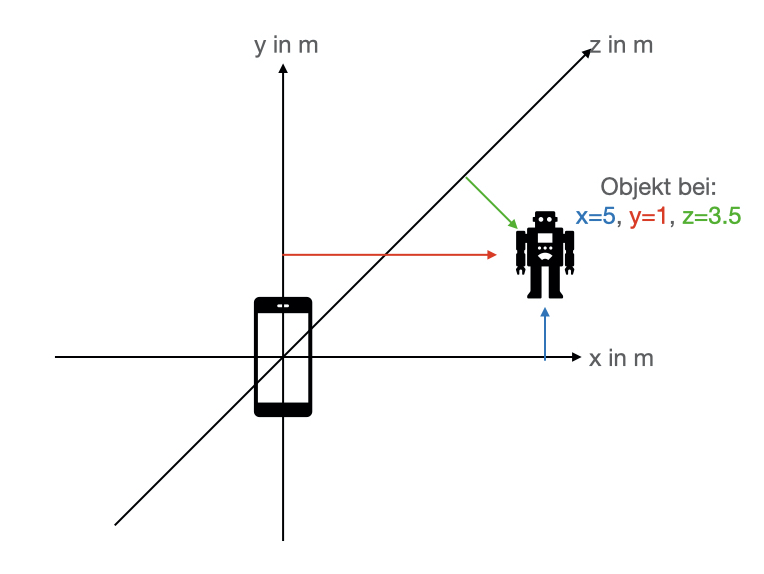
\includegraphics[width=10cm,height=10cm,keepaspectratio]{4Umsetzung/Bilder/koordin.jpeg}
    \caption{Aufbau der Positionsberechnung von Objekten}
    \label{pic:koordin}
\end{figure}
\pagebreak
\\ 
\linebreak
Beim Setzen eines Objekts wird als Anhaltspunkt der Mittelpunkt des Bildschirms berechnet, um das Objekt auf dem Bildschirm zentriert platzieren zu können. Ist 
diese Position berechnet, folgt durch Hilfe des \acs{SLAM} Verfahrens die genaue Ermittlung der virtuellen Position. Anhand der Information dieser Position 
ist das Objekt zu platzieren. 
\\ 
Das Objekte wird gesetzt, indem der Nutzer in der \acs{UI} (\ref{pic:scan}) im Bereich der „Gallery“ ein Objekt anklickt.
Über die der Sceneform-\acs{API} zur Verfügung gestellten Methode („ModelRenderable“) wird das Objekt erschaffen und als „Anchor“ auf die berechnete Position 
gesetzt. Ein Anchor ist die fixe Position des Objekts, an dem dies platziert wird und so lange dort vorhanden bleibt, bis die Applikation beendet wird. Die Datei, 
die als dreidimensionales „asset“ generiert werden soll, wird über die „uri“-Variable lokalisiert und als Parameter übergeben. 
\begin{lstlisting}[language=C,
    frame=lines,           % Ein Rahmen um den Code (single for box, lines for top and bottom)
    xleftmargin=\parindent,  % Rahmen link von den Zahlen
    style=algoBericht,
    label={code:modelrenderable},
    captionpos=b,           % Caption unter den Code setzen
caption={ModelRenderable Builder}]
ModelRenderable.builder()
.setSource(owner.get(), uri)
.build()
.handle((renderable, throwable) -> {
    ...
}
\end{lstlisting}
Während der Objekt-Renderung öffnet sich die \acs{GUI} (\ref{pic:createObject}) zur Eingabe der Informationen, die sich auf das Objekt beziehen. Diese 
werden dann zusammen mit der virtuellen Position des Objekts abgegriffen und in die Datenbank geschrieben. Drückt der Anwender den „save“-Button der Oberfläche 
(\ref{pic:createObject}), beendet er diesen Vorgang und kehrt auf die \acs{UI} der Scan-Phase zurück, um weitere Objekte platzieren zu können. 
\\ 
Zusätzlich zu der Position des Objekts wird dessen Rotation durch Quaternionen berechnet und in der Datenbank gespeichert, um anhand der Berechnung 
die Darstellung so real wie möglich wiederzugeben. Da die Rotation ausgehend von der Kamerahaltung berechnet wird, wird das Objekt bei der Ankerung immer in 
Blickrichtung der Kamera positioniert.
%--> Problemschilderung der Speicherung der Session 
\\ 
\linebreak
Ursprünglich war geplant, die generierte Session sowie die darin erstellten Objekte in der Datenbank abzuspeichern, um diese bei erneutem Aufruf der 
Scan-Phase, bzw. bei Anwendung der Visualisierungs-Phase zu laden und innerhalb dieser Session wieder anzeigen zu lassen. Da die Datenbank nur gewisse Datentypen 
zulässt, war die erste auftretende Schwierigkeit, die Speicherung der Session als Objekt, die zunächst in eine „BLOB“-Datei hätte konvertiert werden müssen. Eine 
„BLOB“-Datei ist ein Binary Large Object, welches anhand der Binärcodierung abgespeichert wird. Dabei kann es sich unter anderem um große 
Bild- oder Audio-Dateien handeln, ebenso können auch mittels dieser Objekt-Konvertierung anderweitig große Dateien gespeichert werden. Daraus entstand die 
Konsequenz, die die Visualisierungs-Phase betraf, nämlich dass eine erzeugte Session nur eine gewissen Zeit verwendet werden kann. Dies bedeutet, dass nach erneutem 
Starten des Assistenzsystems alle zuvor erzeugten Objekte einer Session auf der ihnen zugewiesenen Position nicht mehr erreichbar sind. Durch die Unterschiedlichen 
Startpunkte, die bei wiederholtem Starten der Anwendung erzeugt werden würden, würde sich die ursprüngliche Ausgangsposition der Applikation verschieben und so auch 
die Objekte an eine fälschliche Position projizieren. Genauer gesagt, müssten die Objekte dann ausgehend von dem neu erzeugten Startpunkt referenziert werden. Somit wäre das 
Ergebnis nicht exakt und könnte keine Anwendung finden, da die Applikation Informationen anzeigen würde, die der Realität nicht entsprechen würden. 
\\ 
Basierend auf dieser Erkenntnis musste umdisponiert und ein neuer Lösungsansatz konzipiert werden. Mit dem Wissen über den aktuellen Stand der ARCore \acs{API} 
galt es eine Lösung zu entwickeln, mit der Positionsinformationen exakt wiedergegeben werden können. 
\\ 
Dieser Ansatz wird nun erläutert.
\\ 
\linebreak
Die Idee war es, einen Fixpunkt zu erstellen, welcher dazu dienen würde, einen immer gleichbleibenden Startpunkt vorzugeben. Dadurch gäbe es keine Unterschiede des 
Ausgangspunktes mehr und der Nutzer könnte trotz seiner aktuellen Position die Anwendung starten. Dazu müsste er beim Start der Applikation an den Ursprungspunkt kehren, 
um daraufhin die Scanfunktion zu beginnen. Für diesen Ansatz würde ein Marker zur Verfügung gestellt werden (siehe Abbildung \ref{pic:initialMarker}), der vor dem ersten 
Gebrauch der Software vom Nutzer an einer Position angebracht wird und an dieser dauerhaft bestehen bleibt. Somit ist ein immer gleichbleibender Ausgangspunkt geschaffen, 
von dem aus die Objekte referenziert werden können. Der durch die Anwendung bestimmte Marker müsste entweder als physikalisches Bild an einer bestimmten Stelle in der Realität 
angebracht werden oder als Bild-Datei auf einem Computer immer vorhanden und an der richtigen Position wiederzufinden sein, um die Genauigkeit zu gewährleisten. 
\begin{figure}[hbt!]
    \centering
    
\includegraphics[width=5cm,height=5cm,keepaspectratio]{4Umsetzung/Bilder/cjt_logo_tracking.png}
    \caption{Marker zur Erkennung der Ausgangsposition}
    \label{pic:initialMarker}
\end{figure}
\\
Zur Umsetzung war es notwendig, eine weitere Funktion zur Applikation hinzuzufügen (siehe Abbildung \ref{pic:image_tracking} 
in Scan-Phase \ref{chap:scan_implementation} Frontend), damit ein Marker verfolgt werden kann. Wird dieser Marker erkannt, folgt die eigentliche Scan-Phase, 
die nach der Umkonzeptionierung sowohl bei der Objektplatzierung als auch bei der Datenspeicherung ebenso überarbeitet wurde. 
\\ 
\linebreak
Angenommen der Nutzer startet die Applikation an einer beliebigen Position im Raum und platziert Objekte an von ihm vorgesehenen Stellen, dann würden die 
Objekte erstellt, aber keinerlei Anhaltspunkte geschaffen werden, um bei nachzutragenden Objekten die gleichen Voraussetzungen des zu referenzierenden Standpunktes 
zu erfüllen. Daher wird bei der Scan-Phase die Methode zur Markererkennung eingebaut, um einen initialen Fixpunkt zu erstellen. Dadurch ist es gewährleistet, 
ausgehend von diesem Punkt erneut Objekte zu platzieren, egal wo im Raum die Applikation gestartet wird. Demnach werden die Objekte immer abhängig zur Position des 
Fixpunktes gespeichert, erstellt und angezeigt. Dies bedeutet, dass die Objekte immer eine Referenz zu dem initialen Marker sind. Auch wenn 
ein Objekt nachträglich hinzugefügt werden soll, ist es lediglich erforderlich, den Marker einzuscannen. Danach begibt sich der Nutzer an den gewünschten Ort im 
realen Raum, an dem das Objekt in der Anwendung platziert werden soll. Jetzt muss er die Umgebung mit der Kamera aufnehmen und, indem er auf den Button für das 
Erstellen des Objekts drückt, dieses virtuell erschaffen. Bei der Erzeugung wird die Position ermittelt und anhand dieser die Differenz, bzw. der 
Abstand zu dem initialen Marker in der Datenbank über einen Schreibbefehl gespeichert. Die Berechnung der Distanz zwischen Objekt und 
Ursprungsmarker erfolgt durch eine präzise Subtraktion, bei der lediglich die Ursprungskoordinaten von den aktuellen Positionskoordinaten subtrahiert werden. 
Dieser Vorgang ist dem folgenden Code-Beispiel (\ref{code:differencetoinitial}) zu entnehmen. Dabei wird das aktuelle Objekt „object“ und das initiale Objekt 
„initialObject“ als Parameter übergeben, die sogenannte „call by Reference“, um die Distanz berechnen zu können. Das Ergebnis wird in mehreren lokalen Variablen 
zwischengespeichert und zum Schluss in eine neue Position „Pose“ mit Translation und Rotation, von der Berechnung durch Quaternionen, ermittelt. Der Rückgabewerte 
dieser Funktion ist demnach eine „Pose“, die nach Aufruf der Methode übergeben und so in der Datenbank mittels „insert“-Befehl hinterlegt wird. 
Die Position und Rotation des einzelnen Objekts ist mit dem Resultat gegeben und kann in der Visualisierungs-Phase verwendet werden.
\\
\linebreak
\begin{lstlisting}[language=C,
    frame=lines,           % Ein Rahmen um den Code (single for box, lines for top and bottom)
    xleftmargin=\parindent,  % Rahmen link von den Zahlen
    style=algoBericht,
    label={code:differencetoinitial},
    captionpos=b,           % Caption unter den Code setzen
caption={Berechnung der Distanz zwischen Marker und Ursprungspunkt}]
public Pose returnValueFromPosition(Object object, Object initialObject){
    float tX = object.getTx() - initialObject.getTx();
    float tY = object.getTy() - initialObject.getTy();
    float tZ = object.getTz() - initialObject.getTz();

    float qX = object.getQx() - initialObject.getQx();
    float qY = object.getQy() - initialObject.getQy();
    float qZ = object.getQz() - initialObject.getQz();
    float qW = object.getQw() - initialObject.getQw();

    float[] rotation = {qX,qY,qZ,qW};
    float[] translation = {tX,tY,tZ};

    return new Pose(translation, rotation);
}
\end{lstlisting}
Zur Veranschaulichung der zuvor beschriebenen Methodik dient die Abbildung (\ref{pic:differenztoinitial}). Durch diese Skizze wird nochmals verdeutlicht, dass 
sich alles in einem erstellten Koordinatensystem abspielt und lediglich die Distanz der einzelnen Objekte zum Marker berechnet und in der Datenbank persistiert 
werden.
\begin{figure}[hbt!]
    \centering
    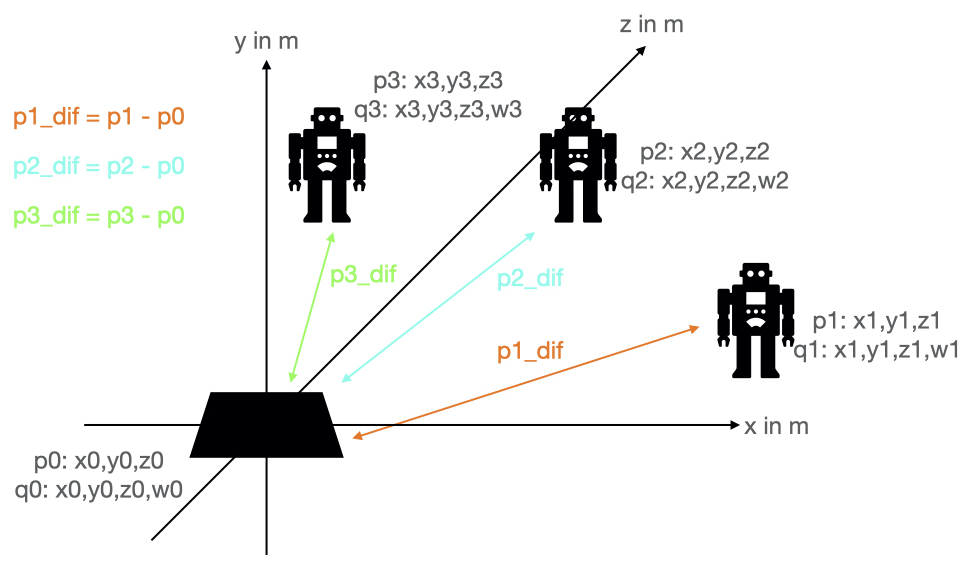
\includegraphics[width=15cm,height=15cm,keepaspectratio]{4Umsetzung/Bilder/difcalc.jpeg}
    \caption{Positionsberechnung zum Ursprungsmarker}
    \label{pic:differenztoinitial}
\end{figure}
\\ 
\linebreak
Um die Backend-Implementierung zu demonstrieren, wird nun während der Laufzeit anhand erstellter Screenshots eine Beschreibung des Ablaufs der Applikation stattfinden.
\\ 
In Abbildung (\ref{pic:markerTracking} (a)) ist zu sehen, dass der vorgegebene Marker verfolgt werden muss, um die Applikation starten zu können. Dabei begrenzt 
die hervorgehobene Umrandung die Fläche, in der der Marker im Bildschirm zur Bildregistrierung platziert werden muss. Nach der Erkennung des Bildes, 
leitet die Benutzeroberfläche automatische auf die eigentliche Ansicht der Scan-Phase um. Ist der Scan aktiviert, folgt die Wahrnehmung der Umgebung durch das 
\acs{SLAM} Verfahren und die Berechnung der vorliegenden Oberflächen. Damit die zu setzenden Objekte exakt auf der Oberfläche des Gegenstandes, der Wand oder dem 
Boden platziert werden können, wird anhand der Sensoren im Smart-Device und dessen Kamera dieser dort berechnet. Dazu wird die berechnete Fläche mit einem Feld voller 
Punkte auf dem Bildschirm überlagert, um dem Nutzer ersichtlich zu machen, 
dass an dieser Position die Schätzung der Oberfläche durchgeführt wurde und die Anwendung darauf ein Objekt platzieren kann. Um dies zu verdeutlichen, wird inmitten 
des Bildschirmes (siehe Abbildung \ref{pic:markerTracking} (b)) ein grüner Punkt angezeigt, der die Platzierung des Objektes vorgibt und dem Nutzer verständlich macht, 
dass ein Objekt erzeugt und an dieser Stelle angesiedelt werden kann. Ist eine Oberfläche der Umgebung noch nicht vollständig berechnet, bzw. erkannt, fehlen 
die Punkte auf dem Bildschirm und es ist lediglich ein grau hinterlegtes Kreuz zu erkennen. Der Nutzer wird dadurch daran gehindert, ein Objekt an einer nicht bekannten 
und nicht berechnet Stelle zu platzieren. 
%Ebenso die zentrierte Markierung, die ein Kreuz vorzeigt, um den Nutzer davor zu hindern ein Objekt an einer nicht bekannten und nicht berechnetet Oberfläche zu platzieren.
\begin{figure}[hbt!]
    \centering
    \subfigure[Marker-Scan]{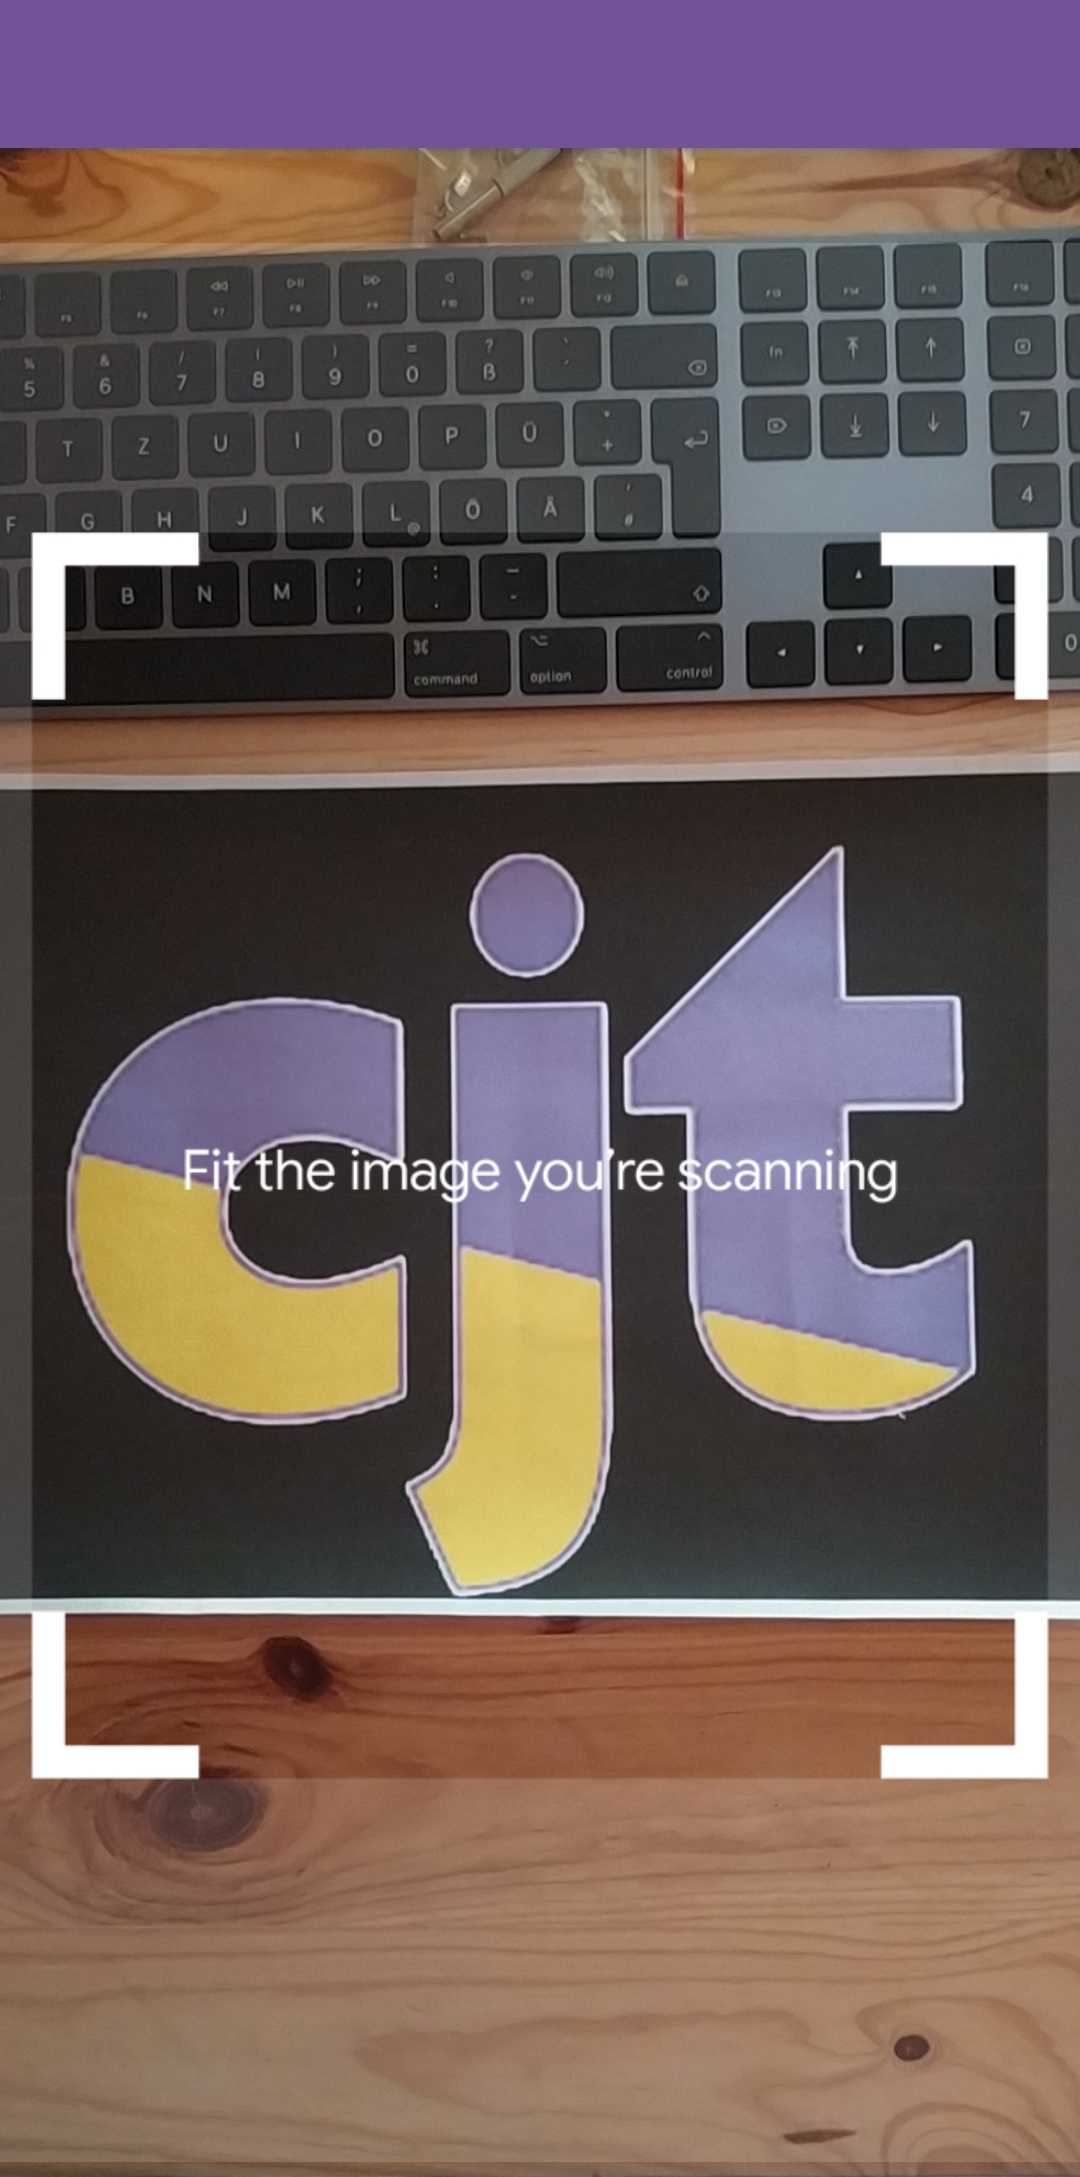
\includegraphics[width=10cm,height=7.5cm,keepaspectratio]{4Umsetzung//Bilder/scan_image.jpg}}
    \subfigure[Umgebungsberechnung]{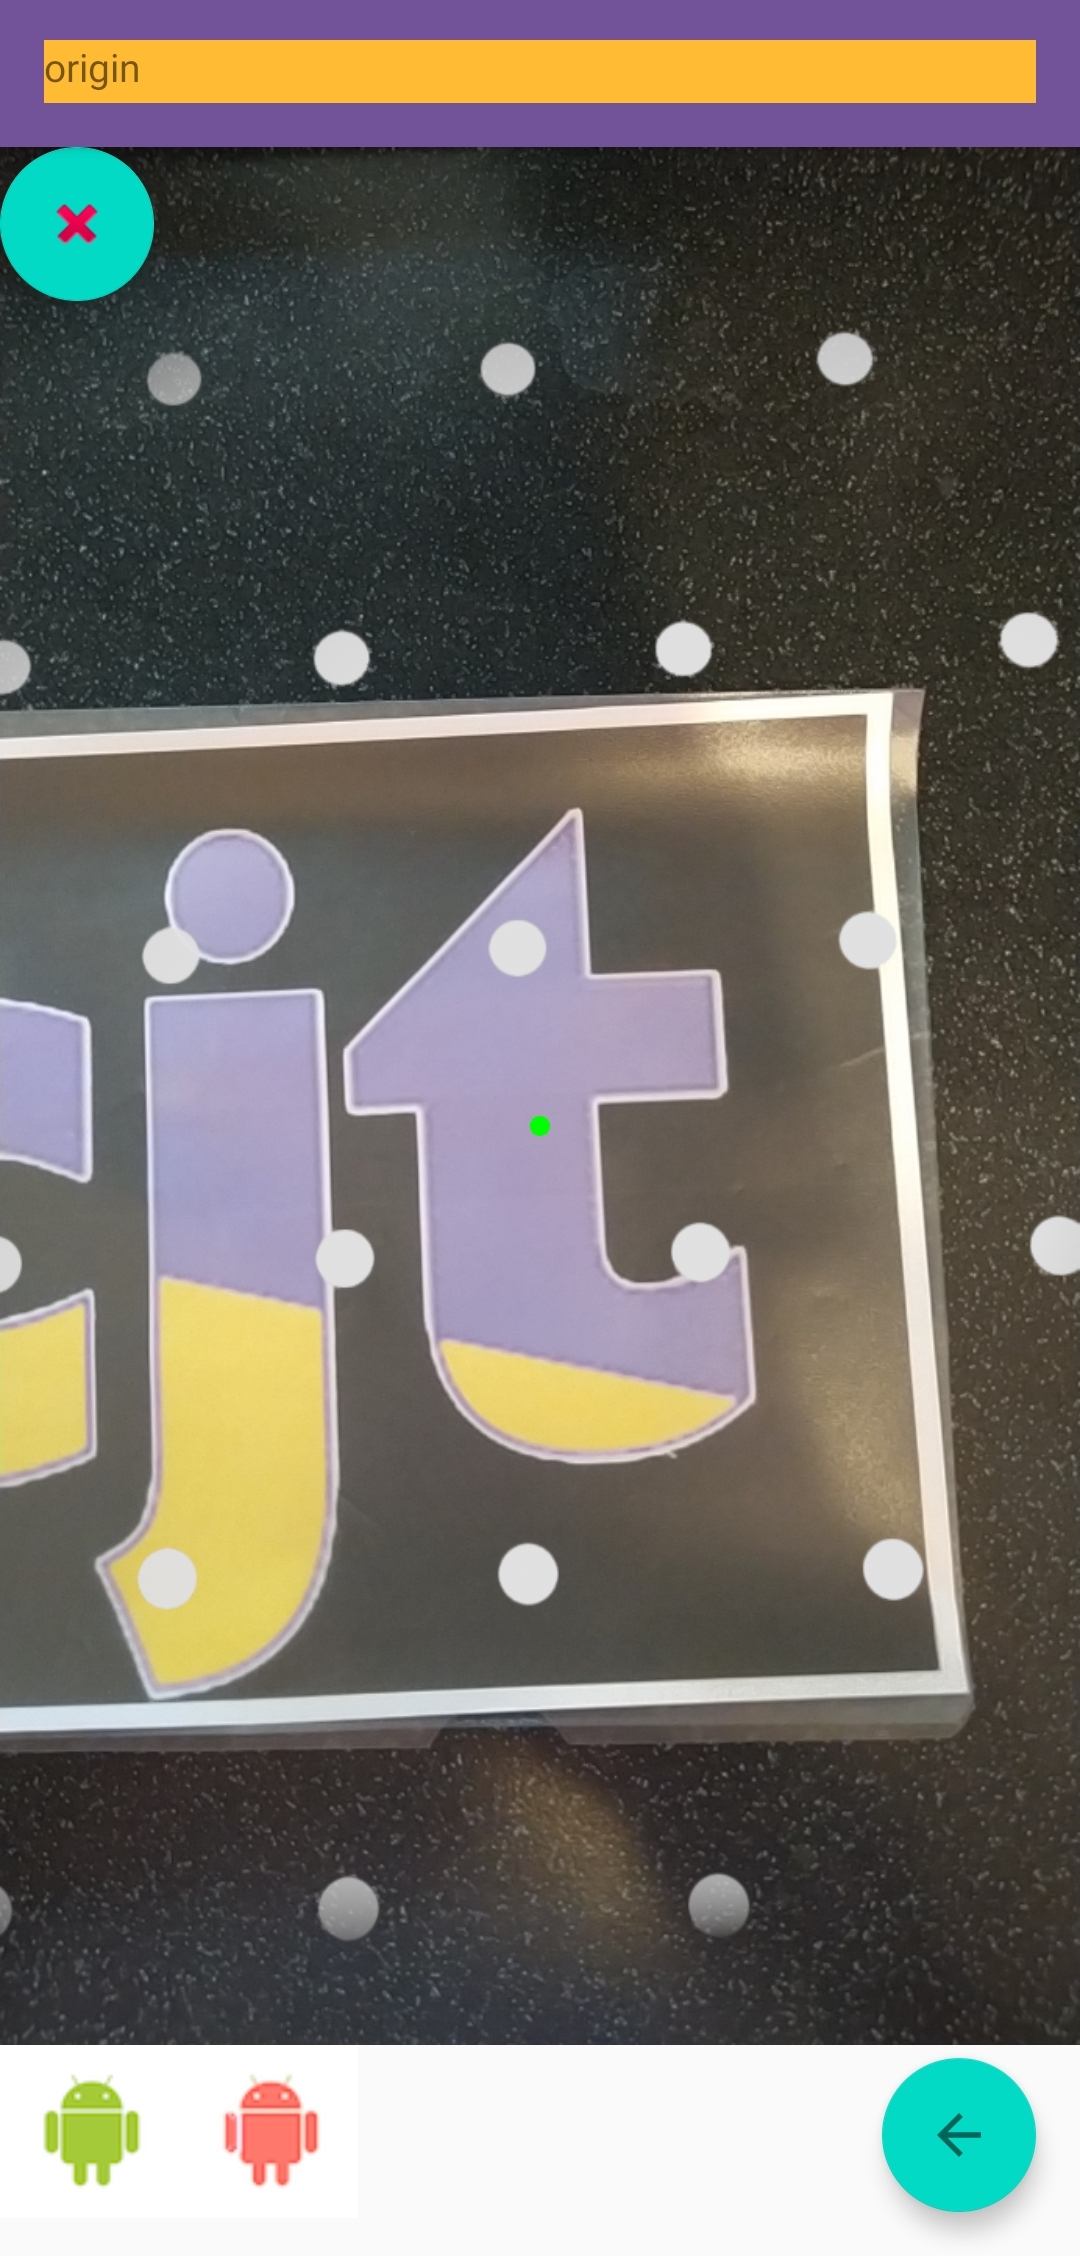
\includegraphics[width=10cm,height=7.5cm,keepaspectratio]{4Umsetzung/Bilder/scan_environment.jpg}}
    \caption{Funktion der Scan-Phase Teil 1}
    \label{pic:markerTracking}
\end{figure}
\pagebreak 
\\ 
\linebreak
Wird nun ein Objekt vom Benutzer erstellt und an eine von ihm gewählte Position platziert, trägt er die dazugehörigen Informationen in der \acs{UI} 
ein, bestätigt diese und übernimmt die Garantie dafür, das Objekt richtig positioniert und betitelt zu haben. Danach wird die ursprüngliche \acs{UI} der Scan-Phase 
geöffnet und das zuvor erstellte Objekt an der vorgesehenen 
Stelle platziert. Demnach können weitere Objekte erzeugt werden. Die folgende Abbildung demonstriert die Darstellung solcher Objekte. Dabei wurden willkürlich 
„Assets" gewählt, die bei tatsächlicher Anwendung in realem Szenario angepasst werden können. Die aktuell verwendeten Objekte fungieren lediglich als 
Veranschaulichung der Aktionen und der Repräsentation des Status eines Objekts. Demzufolge ist der Abbildung (\ref{pic:place_objects}) die Erstellung und 
Darstellung solcher Objekte zu entnehmen. 
\\ 
\linebreak
Hat der Nutzer alle gewünschten Objekte platziert, kann dieser über den Button, rechts unten, die Funktion der Scan-Phase verlassen und die 
Visualisierungs-Phase starten oder die Anwendung schließen. Da alle eingegebenen Informationen persistiert sind, gehen diese nicht verloren und können jederzeit 
über die Visualisierungs-Phase aufgerufen werden. Ist dem Nutzer allerdings ein Fehler bei der Erstellung der Objekte unterlaufen, hat er nach aktuellem Stand 
die Möglichkeit, alle vorhandenen Objekte und Daten zu löschen und die Scan-Phase von Anfang an erneut zu starten.  
\begin{figure}[hbt!]
    \centering
    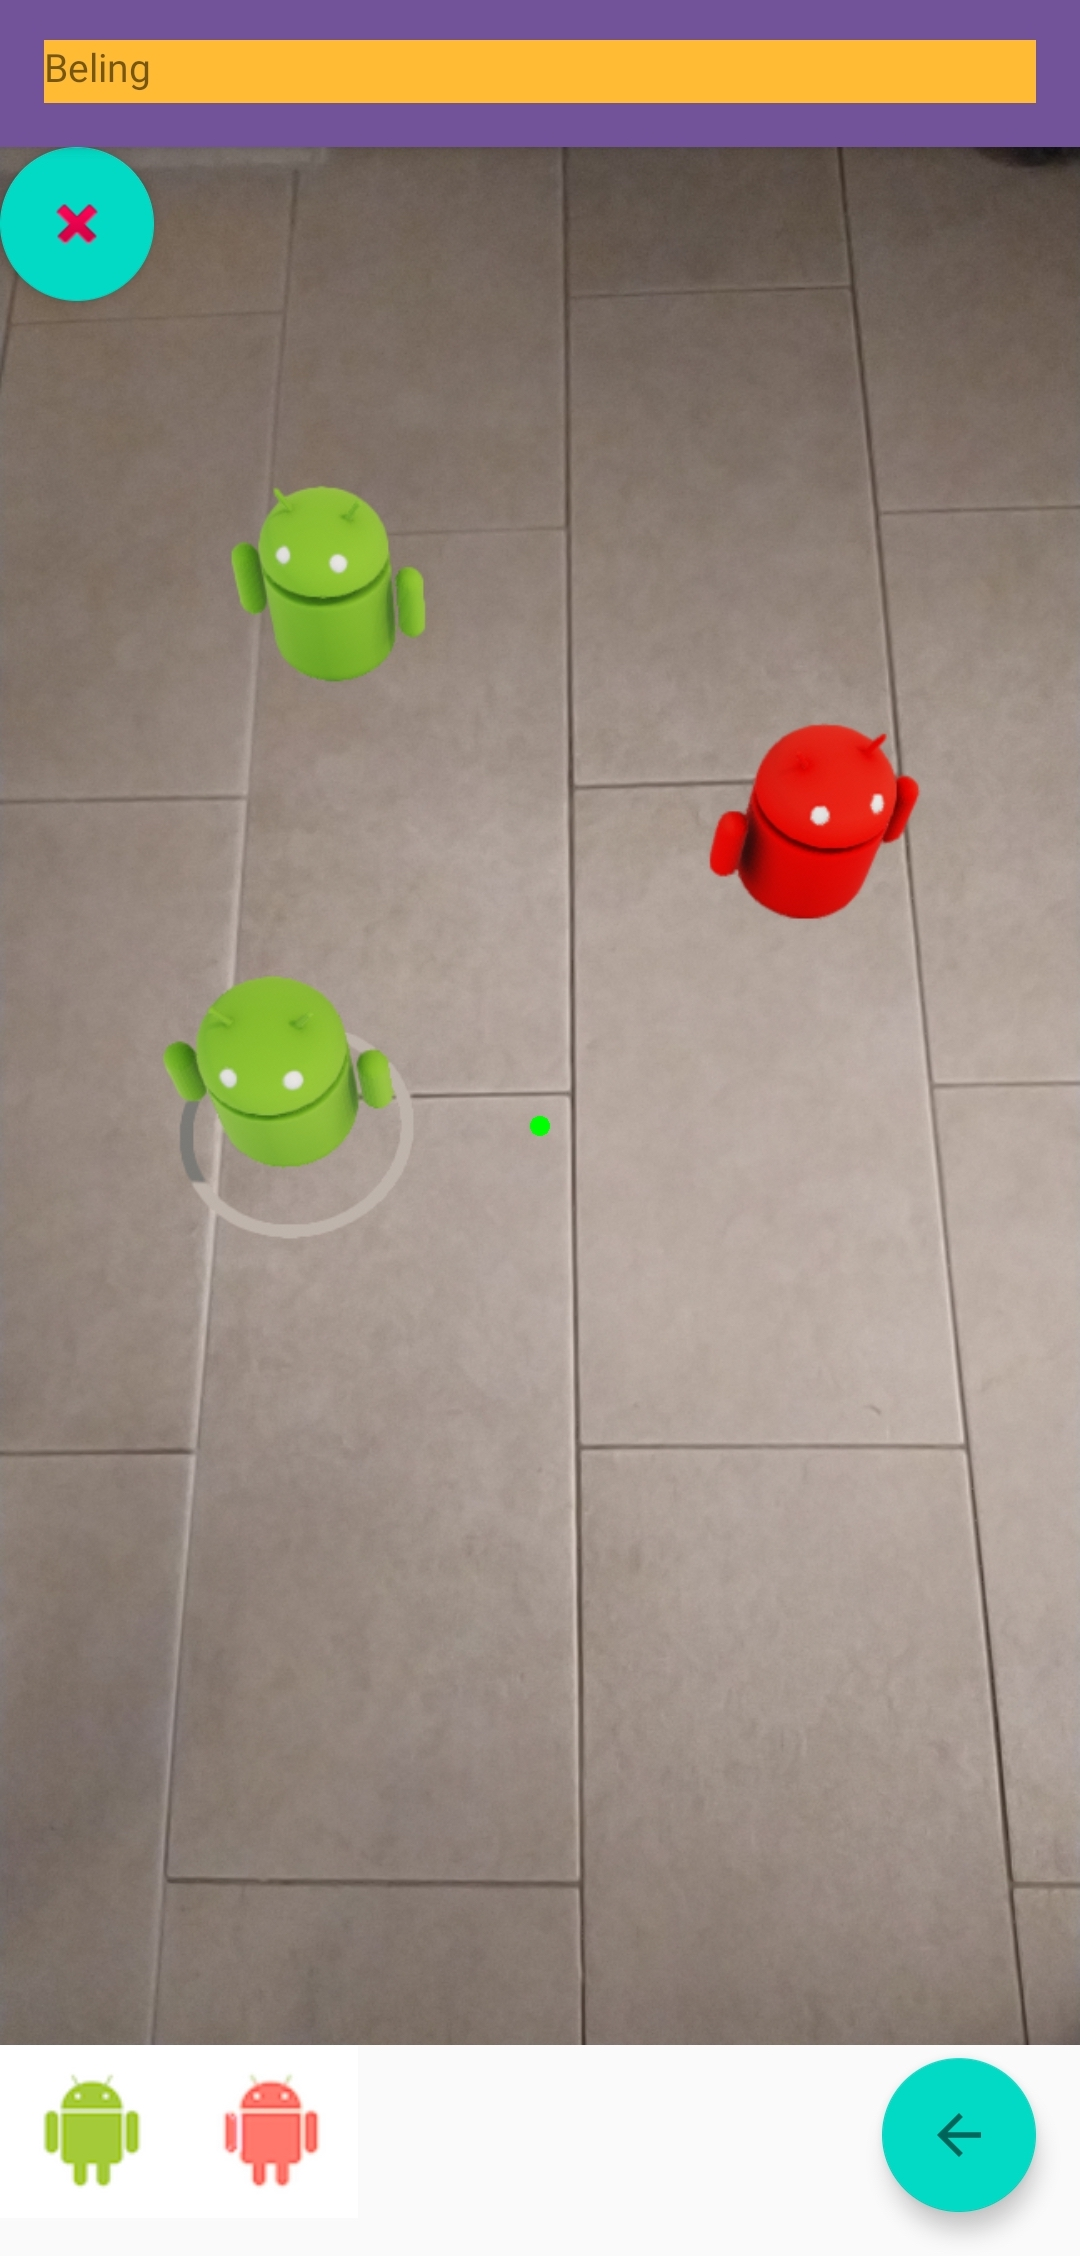
\includegraphics[width=10cm,height=7.5cm,keepaspectratio]{4Umsetzung/Bilder/place_objects_view.jpg}
    \caption{Funktion der Scan-Phase Teil 2}
    \label{pic:place_objects}
\end{figure}
\pagebreak
\\ 
\linebreak
Nachdem die Scan-Phase nun vollends beschrieben wurde, geht es in folgendem Kapitel um die Erläuterung des dritten und letzten Use Cases. Dabei werden sowohl 
die Frontend als auch die Backend Aspekte aufgezeigt. Ebenso wird die Funktionsweise der Objekt-Repräsentation anhand eines kleinen Beispiels, ähnlich wie bereits in 
der Scan-Phase erläutert, veranschaulicht.

\subsection{Visualisierungs-Phase} 
Nach vollständiger Beendigung der Scan-Phase ging es in der Entwicklung weiter mit der Visualisierungs-Phase. Die zuvor gespeicherten Objekte und 
deren Informationen werden dabei abgerufen und können jederzeit erneut visualisiert und im Raum platziert werden. Die folgende Darlegung der 
Frontend-Entwicklung der Visualisierungs-Phase gibt Aufschluss über die Benutzeroberfläche dieser Phase und deren Aufbau. Die Ausführung des Frontends und deren bildliche 
Darstellung dient dazu, das anschließende Backend nachvollziehen zu können. Abschließend werden die Aspekte des Frontends aufgegriffen und anhand der Backend-Implementierung 
mit deren Funktionen verknüpft. 
\subsubsection{FrontEnd}
Bei der Visualisierungs-Phase gibt es prinzipiell eine Benutzeroberfläche, die diesen Use Case ausmacht. Unter eigentlicher Anwendung dieser Phase und 
deren \acs{GUI} befinden sich darüber hinaus weitere Benutzeroberflächen, die bereits in der Scan-Phase schon erläutert wurden. Darunter zum Beispiel 
die in Abbildung (\ref{pic:image_tracking}) zu entnehmende Markererkennungs-\acs{UI}, die ebenso Bestandteil der Visualisierungs-Phase ist. 
\\ 
Die primäre \acs{GUI} ist ähnlich zu der Benutzeroberfläche der Scan-Phase aufgebaut. Ein Fragment das sich über den ganzen Bildschirm erstreckt, repräsentiert das 
Livebild der Kamera. Dadurch können die bereits in der Scan-Phase erstellten Objekte erneut angezeigt werden. Des Weiteren befinden 
sich auf dieser Oberfläche zwei Buttons, zum einen zur Navigation, um auf das Startmenü zu gelangen, und zum anderen, um die Objekte von der Datenbank 
abzugreifen, rendern und auf dem Bildschirm anzeigen zu lassen. Diese befinden sich jeweils in der linken und rechten unteren Ecke des Bildschirms, wie 
der Abbildung \ref{pic:visual} zu entnehmen ist. 
\\ 
Da diese \acs{UI} nur als Ansicht der zu visualisierenden Objekte gedacht ist, stehen dem Nutzer für die Interaktionen nur die Objekte, die als Overlay 
über das Kamerabild gelegt werden, zur Verfügung. Die Nutzeraktionen beschränken sich lediglich auf den Gebrauch der zuvor genannten Buttons und die dynamisch erzeugten 
Schaltflächen der Objekte, um über diese zusätzliche Informationen zu erhalten. 
\begin{figure}[hbt!]
    \centering
    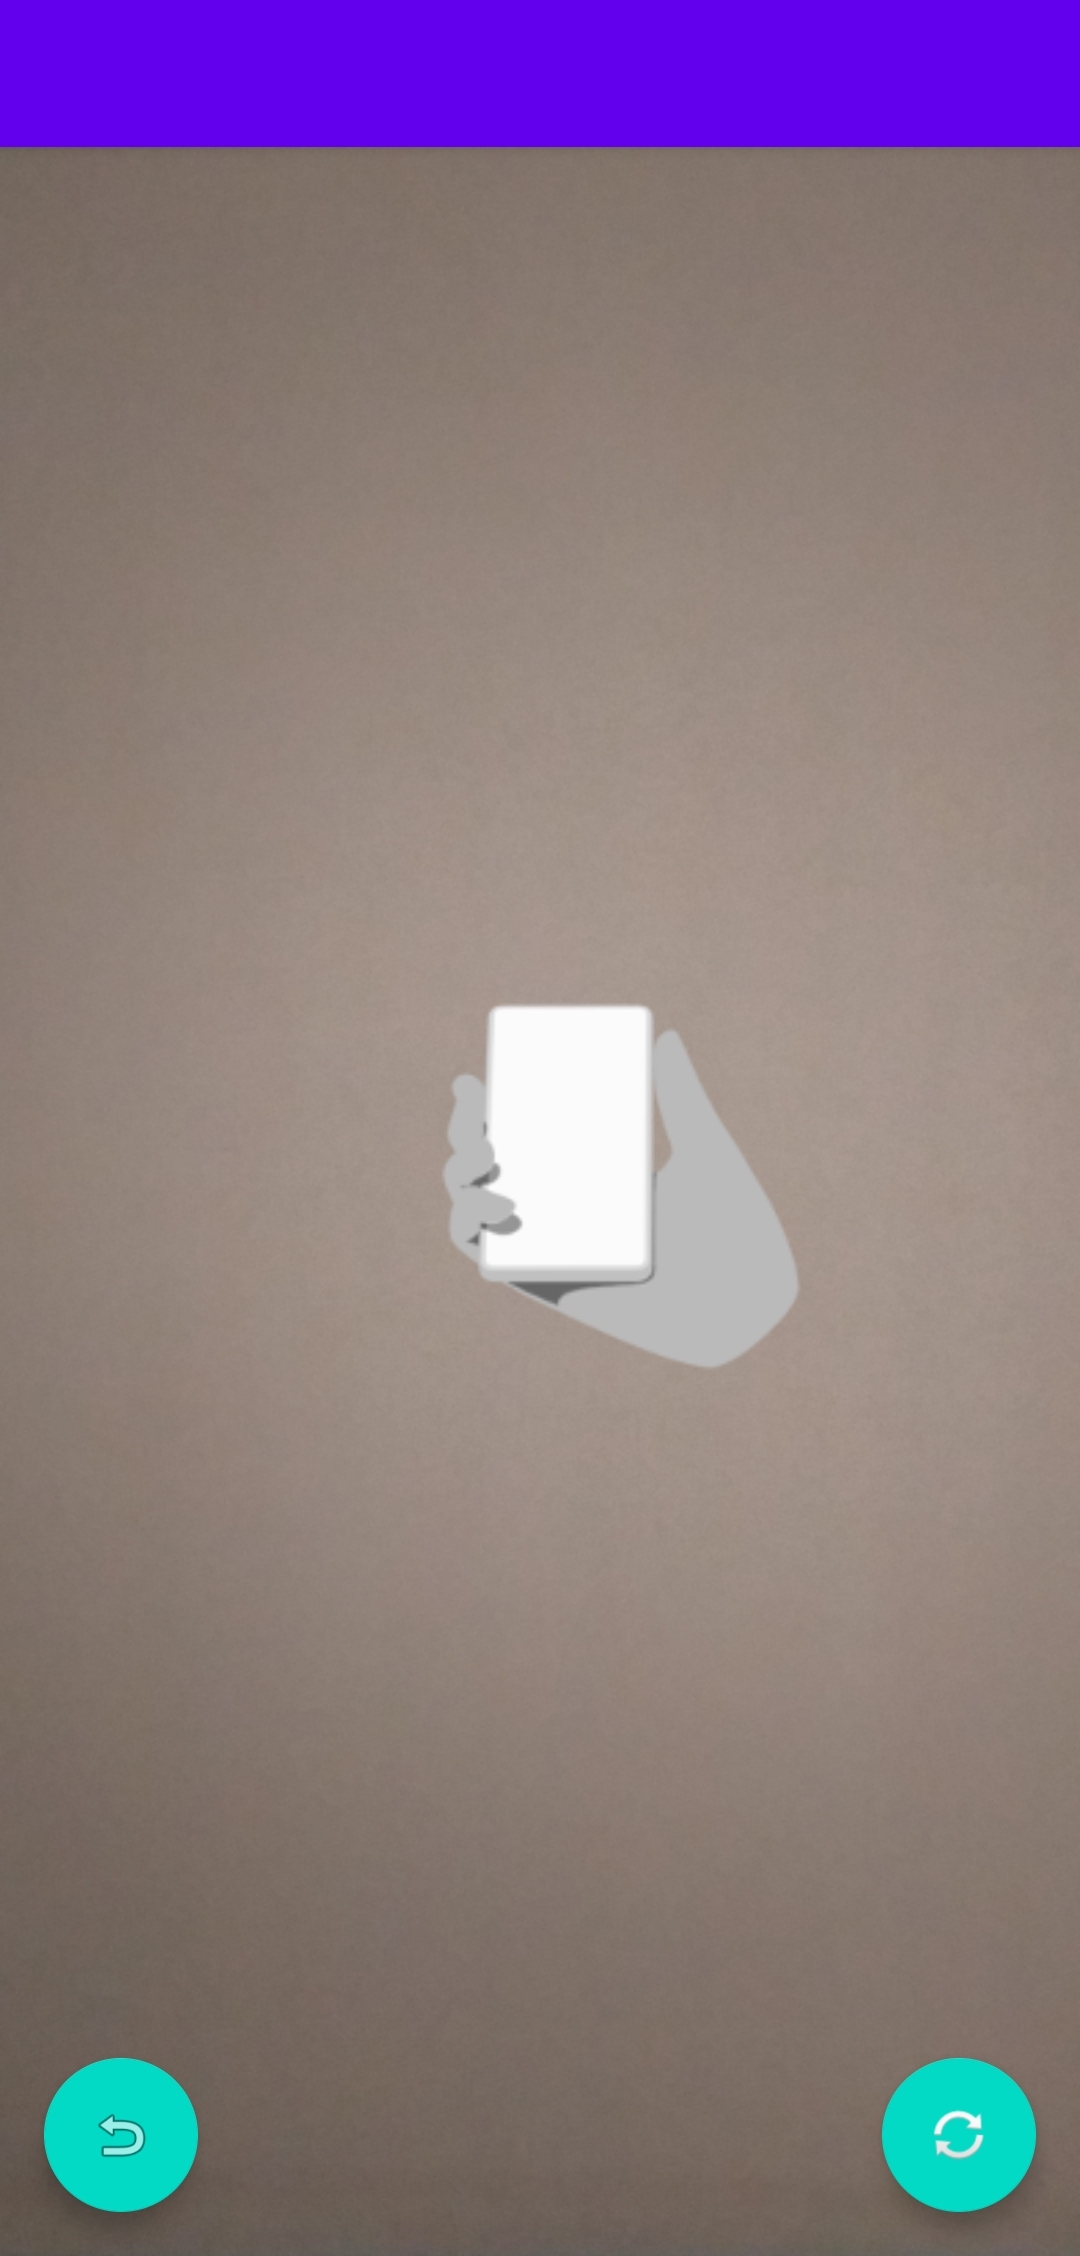
\includegraphics[width=10cm,height=7.5cm,keepaspectratio]{4Umsetzung/Bilder/visual-phase.jpg}
    \caption{Visualisierungs-Phase der Applikation}
    \label{pic:visual}
\end{figure} 
\\
Nun erfolgt die Beschreibung der Backend-Implementierung und Einblicke in die Programmierung der Visualisierungs-Phase.  
% \subsubsection{BackEnd}
Nachdem das Problem der variablen Startposition in der Implementierung der Scan-Phase umgangen wurde, konnte die Visualisierungs-Phase entwickelt werden. 
\\ 
\linebreak
Wählt der Anwender auf der Startmenü-\acs{UI} (\ref{pic:startmenu}) den Button „Virtual-Phase“, wird eine Anmerkung getätigt, indem der Nutzer darüber in 
Kenntnis gesetzt wird, dass er zu Beginn die Scan-Phase durchgeführt haben muss, bevor die Visualisierungs-Phase gestartet werden kann. Diesen Vermerk kann der 
Benutzer ignorieren, wenn dieser weiß, dass ein Scan durchgeführt wurde, oder er akzeptiert den Hinweis und wird auf die dementsprechende Funktion weitergeleitet. 
Der Nutzer wird dadurch davor bewahrt, eine Funktion starten zu wollen, die ohne Inhalt keine Änderungen aufzeigt.
\\ 
Danach wird der Nutzer aufgefordert, den initialen Marker (\ref{pic:initialMarker}) einzuscannen, um die ursprüngliche Position, bzw. die Markierung festzuhalten. 
Damit kann der weitere Programmablauf folgen, indem die \acs{GUI} der Visualisierungs-Phase (\ref{pic:visual}) angezeigt und eine neue Session zur 
Objektplatzierung gestartet wird. 
\\
Über eine ViewModel-Komponente werden die Objekte aus der Datenbank abgefragt und in einer Liste gespeichert, um diese zu einem späteren Zeitpunkt zur Platzierung der 
Objekte verwenden zu können. 
\\ 
Ist der Marker erkannt worden, wird mithilfe des Buttons, der sich im rechten unteren Eck der Benutzeroberfläche (\ref{pic:visual}) befindet, die Methode zur 
Datenabfrage, Erzeugung und Platzierung der Objekte gestartet. Dabei wird über den Button-Klick eine Funktion aufgerufen, die die Liste der Objekte anspricht und 
die jeweils darin enthaltenen Objekte nacheinander generiert. Nach Betätigen des Buttons ist dieser auf der \acs{UI} nicht mehr aufzufinden, um einer weiteren 
Platzierung aller Objekte vorzubeugen. Die von dem ViewModel gegebene Liste wird, abhängig von deren Länge, iterativ abgearbeitet und die Objekte 
nacheinander angelegt. Dies erfolgt über eine „for“-Schleife, welche abhängig von dem Ursprungspunkt, dem Marker „objectMarkerCenter“, die Position des 
aktuellen Objekts „obj“ an der Stelle „i“ in der Liste neu errechnet und darstellt.
\\ 
\linebreak
\begin{lstlisting}[language=C,
    frame=lines,           % Ein Rahmen um den Code (single for box, lines for top and bottom)
    xleftmargin=\parindent,  % Rahmen link von den Zahlen
    style=algoBericht,
    label={code:listOfObjects},
    captionpos=b,           % Caption unter den Code setzen
caption={Abfolge der Objekte in der Liste}]
... 
for (int i = 1; i < listOfObj.size(); i++){
    obj = listOfObj.get(i);
    if(!obj.getName().equals("origin")) {
        calculateObjectPosition(obj, i, objectMarkerCenter);
    }
}
\end{lstlisting}
Mit der gegebenen „calculateObjectPosition“ wird dann die Distanz vom Ursprungsmarker zu dem Objekt addiert, um 
die Positionen und Distanzen der einzelnen Objekte der Scan-Phase exakt wiederzugeben. Ist die Addition zu einem Objekt durchgeführt, repräsentiert diese 
Berechnung unabhängig von der Startposition des Anwenders die neue Position, an der das Objekt platziert werden muss. Somit ist der Nutzer bei Verwendung der 
Applikation in der Lage, aus einem vorab beliebigen Punkt zu starten und alle Objekte exakt auf die referenzierte, ursprüngliche Position zu setzen, die 
in der Scan-Phase festgelegt wurde. Nachdem die Position des aktuellen Objekts berechnet wurde, wird diese als neue „Pose“ initialisiert und übergeben, um 
das zu erstellende Objekt zu rendern und auf der Oberfläche anzuzeigen. Dabei findet eine Abfrage des Status statt, um daraufhin 
entscheiden zu können, in welcher Farbe das Objekt zu Präsentieren ist.  
\\ 
\begin{lstlisting}[language=C,
    frame=lines,           % Ein Rahmen um den Code (single for box, lines for top and bottom)
    xleftmargin=\parindent,  % Rahmen link von den Zahlen
    style=algoBericht,
    label={code:additionOfObject},
    captionpos=b,           % Caption unter den Code setzen
caption={Berechnung der Markerplatzierung}]
public void calculateObjectPosition(Object object, int i, Object objOrigin){
    ... 
    qx = object.getQx() + objOrigin.getQx();
    qy = object.getQy() + objOrigin.getQy();
    qw = object.getQw() + objOrigin.getQw();
    qz = object.getQz() + objOrigin.getQz();

    tx = object.getTx() + objOrigin.getTx();
    ty = object.getTy() + objOrigin.getTy();
    tz = object.getTz() + objOrigin.getTz();

    float[] rotation = {qx,qy,qz,qw};
    float[] translation = {tx,ty,tz};

    Pose pose = new Pose(translation, rotation);

    if(objectViewModel.getAllObjectsName().getValue().get(i).getState() == 1) {
        addObject(Uri.parse("object.sfb"), pose, i);
    }

    if(objectViewModel.getAllObjectsName().getValue().get(i).getState() == -1){
        addObject(Uri.parse("object_red.sfb"), pose, i);
    }
}
\end{lstlisting}
Sind alle Listenelemente abgearbeitet, ist die Erstellung und Renderung der Objekte fertig. Danach werden dem Nutzer alle vorhandenen Objekte angezeigt und 
visualisiert. Mit diesen Erkenntnissen kann der Nutzer durch den Raum laufen und alle Objekte überwachen. Wird ein Objekt anvisiert, kann über eine Berührung 
des Objekts auf dem Display alle vorhandenen Informationen eingesehen werden. Somit sind die Informationen des einzelnen Objekts schnell sichtbar.  
Die Applikation kann beliebig oft geschlossen und neu gestartet werden. Der Nutzer kann sich zu jeder Zeit die Objekte visualisieren lassen, vorausgesetzt, der 
Ursprungsmarker wird zu Anfang eingescannt. Daraufhin können alle Objekte präsentiert und die dazugehörigen Informationen angezeigt werden. %  zu jeder Zeit
\\ 
\linebreak
Um die soeben beschriebene Backend-Implementierung der Visualisierungs-Phase zu demonstrieren, wird diese anhand eines kleinen Szenarios veranschaulicht. 
\\ 
Startet der Nutzer die Visualisierungs-Phase, muss er den initialen Marker scannen, um fortfahren zu können. Darauffolgend öffnet sich die \acs{GUI} dieser 
Phase und mit einem Klick auf den Button rechts unten auf der Oberfläche synchronisiert er die Funktion und alle Objekte, die in der Scan-Phase gesetzt wurden, 
werden erneut generiert. Daraufhin kann der Nutzer die Objekte an den Stellen einsehen, an denen sie sich ursprünglich befanden. So werden diese samt Status 
angezeigt und der Nutzer hat den gesamten Überblick über alle Objekte und kann diese beobachten. Der Schritt ist der Abbildung (\ref{pic:visual_objects}) 
zu entnehmen. 
\begin{figure}[hbt!]
    \centering
    \includegraphics[width=10cm,height=7.5cm,keepaspectratio]{4Umsetzung/Bilder/show_objects_after_loading.jpg}
    \caption{Funktion Visualisierungs-Phase Teil 1}
    \label{pic:visual_objects}
\end{figure}
\\ 
\linebreak
Eine weiter Funktion dieser Phase ist die Verwaltung der Objekte und deren Informationen. Wird ein Objekt anvisiert, werden mit einem Klick auf das Objekt 
die Informationen über ein PopUp angezeigt. Darunter ist der Namen des Objekts, der Status und die ID, die zu Anfang automatisch generiert 
und vergeben wurde. So kann zu jedem einzelnen Objekt dessen Informationen zur Verfügung gestellt werden. 
\pagebreak
\begin{figure}[hbt!]
    \centering
    \subfigure[Anzeige der Objektinformationen 1]{\includegraphics[width=10cm,height=7.5cm,keepaspectratio]{4Umsetzung//Bilder/show_data_to_obj_1.jpg}}
    \subfigure[Anzeige der Objektinformationen 2]{\includegraphics[width=10cm,height=7.5cm,keepaspectratio]{4Umsetzung/Bilder/show_data_to_obj_2.jpg}}
    \subfigure[Anzeige der Objektinformationen 3]{\includegraphics[width=10cm,height=7.5cm,keepaspectratio]{4Umsetzung/Bilder/show_data_to_obj_3.jpg}}
    \caption{Funktion Visualisierungs-Phase Teil 2}
    \label{pic:showdatatoobj}
\end{figure}
\\ 
\linebreak
Nachdem die Aspekte der Front- und Backend-Entwicklung der drei Use Cases geschildert und Einblicke in die Entwicklung und die damit verbundenen Fragestellungen 
und Schwierigkeiten gewährt wurden, geht es nun mit der Evaluierung des Systems, dem Fazit und dem Ausblick weiter.

%werden die implementierten Funktionen anhand eines Testdurchlaufs nochmals genauer 
%dargelegt.
%\section{Testdurchlauf} %/ Test-Szenario
%\label{chap:testdurchlauf}
%Ergänzend zur Implementierung wird in diesem Abschnitt das Resultat und die Anwendung der Applikation anhand eines unabhängigen Tests praktiziert, um die 
%Erzeugnisse der Entwicklung darzustellen und gegebenenfalls erweiternd zur eigentlichen Entwicklungsbeschreibung Ergebnisse zu präsentieren.
% \chapter{Evaluation}
\label{chap:Evaluation}
Nach Beendigung der Entwicklungsphase wurde eine Evaluation des Softwareprodukts durchgeführt. Diese dient zur Kategorisierung und Einstufung der Applikation in 
die Gebrauchstauglichkeit. Dabei wurde auch ein Vergleich zu schon bestehenden, bzw. ähnlichen Produkten aufgestellt. Darunter befinden sich 
ebenso Aspekte der Benutzerfreundlichkeit, der Weiterentwicklungsmöglichkeiten und eine Überprüfung auf gewünschte, bzw. vorab definierte Anforderungen 
und Ziele. 
\\ 
\linebreak
Im Bereich der Industrie gibt es derzeit einige Anwendungen, die auf \acl{AR} aufbauen, darunter sind allerdings wenige Apps, die sich mit vorliegenden Prozessen 
auseinandersetzen. Es gibt vereinzelt Anwendungen, die mit Interaktionen in Prozessabläufen arbeiten. Diese basieren allerdings weniger auf 
einer Smartphone-Applikation. Es wird vermehrt auf \acs{VR}- und \acs{AR}-Brillen gesetzt. Diese sind meist für die Begleitung der 
Prozesse zuständig und projizieren zusätzliche Informationen oder Visualisierungen, um dem Nutzer erweiterte Einblicke zu verschaffen. Es gibt auch 
Anwendungen die visualisierte Arbeitsprozesse vorgeben, und das Potenzial, den Effekt und die Effizienz des „learning by doing“-Ansatzes ausschöpfen oder auch 
Vorstellungen und Planungen zum besseren Vorstellen visualisieren. Beispiele dazu sind zum einen der „augmented presenter“ \cite{tepcon.2020} 
und der „augmented instructor“ \cite{tepcon.2020} der tepcon GmbH. Der „augmented presenter“ bietet die Möglichkeit, eine Inneneinrichtung einer Produktionshalle 
zu visualisieren und damit Maschinen an verschiedenen Stellen zu platziert. Anhand dieser Projektion wird überprüft, ob sich die vorgesehene Position 
für die Platzierung der zu planende Maschine eignet. Diese Anwendung dient zur optimierten Fabrikplanung, bevor die Produkte bestellt oder in Betrieb genommen 
werden. Auch kann diese Anwendung für Vertrieb und Marketing, Schulungen und Messen zur Demonstration der Möglichkeiten der \acs{AR} verwendet werden. Der 
„augmented instructor“ basiert auf dem Gebrauch der \acs{AR}-Brille und visualisiert und projiziert Arbeitsschritte zur Veranschaulichung. 
\\ 
\linebreak
Das entwickelte, prototypische Assistenzsystem dient zur übersichtlichen Verdeutlichung der vorhandenen Maschinen in einer Produktionshalle. Dadurch kann die 
Umgebung eingescannt und Maschinen als Objekte virtuell dargestellt werden. Mit den nötigen Daten ermöglicht dieses System die schnelle Abrufung von Informationen 
zu einzelnen Maschinen. Auch die Option der Echtzeit-Statusüberprüfung kann in weiterer Entwicklung realisiert werden. 
\\ 
So kann das Assistenzsystem schnell Informationen zur Verfügung stellen, die immer verfügbar sind. Durch die einfache Erweiterbarkeit, die 
durch die Architektur gewährleistet ist, können weitere nützliche Funktionen hinzugefügt werden und bestätigt dessen stetig erweiterbare Alltagstauglichkeit.
\\ 
Auch im Hinblick auf die Benutzerfreundlichkeit ist eine einfache \acs{UI} gegeben, die überschaubar und schnell zu verstehen ist. Die Norm ISO 9241-10 schreibt eine gute 
Steuerbarkeit, Selbstbeschreibungsfähigkeit, Individualisierbarkeit und Aufgabenangemessenheit vor. In der Entwicklung der Anwendung wurde versucht, sich daran zu orientieren. 
In Usability-Tests wurden die Anforderungen der Norm in kleinem Rahmen, aber noch nicht abschließend, überprüft. Auf diese Tests wird im Folgenden aus Relevanzgründen nicht 
näher eingegangen. Im Rahmen der Testungen wurden 
Verbesserungsvorschläge geäußert, die sich in diesem Bezug nur auf Erweiterungen bezogen haben. Ebenso wurde die Genauigkeit bemängelt, da 
diese manchmal fehlerhaft Objekte erstellt und wiedergibt. Die Ursache ist der Handhabung durch den Nutzer zuzuschreiben, der je nach Lage und Ausrichtung des Smart-Device 
die Berechnung beeinflusst. 
\\ 
In der Gesamtheit wurde das System als überaus hilfreich und entwicklungsfähig eingestuft. In dieser Arbeit stehen lediglich die Konzeption, 
Grundlagenschaffung und prototypische Entwicklung im Fokus. Die Grundfunktion wurde implementiert und zur Verfügung gestellt.
\\ 
\linebreak
Nun folgt abschließend, um die Dokumentation abzurunden, das allgemeine Fazit des Projekts und der Ausblick, der die Zukunftsaussichten des Projekts darlegt. 
\chapter{Fazit}
\label{chap:Fazit}
Ziel dieser Arbeit war die Konzeption und prototypische Umsetzung eines Assistenzsystems zur Unterstützung industrieller Prozesse. Dabei wurde der Fokus auf die 
übersichtliche und virtuelle Darstellung von Maschinen und Geräten gelegt. Zu der Übersicht kam auch dazu, dass zu einzelnen Objekten schnell Informationen eingesehen 
werden können, um diese bei Bedarf zur Hand zu haben. Dafür wurden in den ersten Schritten Anforderungen zur Umsetzung des Systems festgelegt. Unter Berücksichtigung der 
zu gewährleistenden Modularisierung musste ein geeignetes Entwurfsmuster gefunden werden, auf dem die Architektur aufbaut, um künftige Weiterentwicklungen an dem Projekt 
zu ermöglichen und diese keine großen Herausforderungen darstellen. Durch die Android Architecture Components wurde sich an dem MVVM-Muster angelehnt, welches unter anderem 
die Anforderungen der Modularisierung erfüllt. Bevor die konkrete Umsetzung stattfinden konnte, wurden anhand der Anforderungen und geplanten Funktionen Use Cases für die 
Implementierung definiert. Nachdem diese modelliert waren, konnte das eigentliche System aufgestellt und entwickelt werden.
\\ 
\linebreak
Die Positionsberechnung des Smart-Devices basiert auf Kalkulationen der hardwareinternen Sensoren und unterliegt somit einer sehr sensiblen Basis. Je nach Ausrichtung und 
Lage des Geräts kann sich sowohl dessen Orientierung, als auch dessen Blickrichtung unterscheiden und so das eigentliche Ergebnis verfälschen, obwohl sich das Gerät an der physikalisch 
identischen Position befindet. Dadurch ist die Benutzung der Applikation stark von den Aktionen und der garantierten Handhabung des Nutzers abhängig. 
\\ 
\linebreak
Das verwendete Framework Google ARCore erweist einen effektiven Nutzen und ist eine gute Grundlage für die Implementierung einer \acl{AR} Applikation. Das 
Framework stellt eine fundamentierte \acs{API} zur Verfügung, die eine gute Basis für die darauf aufbauenden Entwicklungen schafft. Bei der praktischen 
Anwendung des Frameworks gibt es jedoch vereinzelt Probleme mit der Anzeige der virtuellen Objekte, da aus den Positionsberechnungen phasenweise Übereinstimmungen mit diesen 
nicht erkannt und dadurch die Objekte nicht angezeigt werden. Daher ist es in diesem Fall notwendig, an den Ausgangspunkt zurückzukehren, damit die 
Anzeige der Objekte aktualisiert werden kann und so die nicht angezeigten Visualisierungen wieder auftauchen.
\\ 
\linebreak
Werden Objekte über die Scan-Phase an eine bestimmte Position gesetzt, wird die daraus resultierende Differenz zum Ursprungsmarker gespeichert. Bei der 
Ausführung der Visualisierungs-Phase werden die gespeicherten Objekte und deren Positionsdifferenz abhängig von der Ursprungsmarkierung wieder virtuell im Raum platziert. 
Dabei ist die Ausgangssituation der Markierungsverfolgung entscheidend. Dies bedeutet, dass das Smart-Device vom Nutzer richtig angewendet werden muss und es beispielsweise 
nicht über Kopf gehalten werden darf. Dadurch würde die Berechnung und Darstellung der Objekte nicht exakt mit der vorgesehenen Position übereinstimmen. Dies hat eine 
ungenauer Repräsentation der Objekte im Raum zufolge. 
\\ 
Es ist durch diese Sensibilität der Anwendung vorauszusetzen, dass der Nutzer das System verantwortungsvoll und gewissenhaft verwendet. Da dies von dem Assistenzsystem nicht überprüft 
und auch nicht korrigiert werden kann, muss die fachgerechte Handhabung vorausgesetzt werden. 
\\ 
\linebreak
Im Großen und Ganzen sind die Benutzeroberflächen überschaubar und bieten eine gute Grundlage für die Anwendung der \acl{AR} Applikation. 
\\ 
\linebreak
In der Gesamtheit bietet das Ergebnis dieser Arbeit einen klaren und leicht verständlichen Aufbau des Systems, sowie eine Grundlage für Weiterentwicklungen. 
Das Konzept wurde eigenständig erarbeitet und wie geplant umgesetzt. Somit ist der Grundbaustein für weitere, darauf aufbauende Funktionen gelegt.

\chapter{Ausblick}
\label{chap:Ausblick}
Der in dieser Arbeit entstandene Prototyp ist ein eigenständiges System zur visualisierten Übersicht von Maschinen und Geräten, beispielsweise in Produktionshallen. 
Bevor die Anwendung allerdings produktiv eingesetzt werden kann, sind noch einige Optimierungen vorzunehmen. Darunter die Verwendung von weiteren Objekten 
zur visuellen Darstellung der Maschinen. Eventuell können auch detailgetreue Abbildungen in einem bestimmten Anwendungsumfeld oder die Verwendung universeller 
ortsunabhängiger Objekte eingesetzt werden. Des Weiteren muss die Überarbeitung der Informationsanzeige der Objekte, die aktuell über ein vereinfachtes Informationsfenster 
eingeblendet werden, erfolgen. Eine \acl{AR} basierte Anzeige der Informationen wäre dabei denkbar. In dieser Arbeit wurden lediglich die Grundsteine für ein Projekt 
gelegt, welches in Zukunft stetig weiterentwickelt werden kann und viel Potential für weitere Funktionen, auf Basis der \acs{AR}-Anwendung, bietet. Die Ergebnisse 
des Prototypen sind für erste Tests geeignet, allerdings für den derzeitigen Einsatz noch nicht vorgesehen. Da zum jetzigen Zeitpunk noch kein Zusatznutzen für Anwender 
daraus resultiert und die maschinenbezogenen Daten im Hinblick auf die statusabhängigen Informationen keine Echtzeit-Auskünfte bietet, ist das Assistenzsystem für Firmen 
noch uninteressant und unrentabel. Der Prototyp muss der Prototyp weiterentwickelt und verbessert werden. 
\\ 
\linebreak
Um Informationen über einzelne Maschinen in Echtzeit aufrufen und visualisieren zu können, wäre ein weiterer Entwicklungsschritt die Benutzung von Echtzeitdaten der 
Maschinen. Dafür wäre eine Datenaufbereitung und eine globale Verfügbarkeit der Informationen notwendig. Diese Idee könnte über eine \acl{IoT}-Lösung, umgesetzt werden. 
Dabei könnten die Maschinendaten, die über eine Cloud ausgelagert sind, in Echtzeit abgegriffen und stets den aktuellen Zustand und Status der einzelnen Geräte 
abgerufen werden. Auch könnten die Daten direkt von den jeweiligen Geräten verwendet, aufbereitet und in der Anwendung genutzt werden. Dadurch wäre die Möglichkeit 
gegeben, genauere Informationen zu den Objekten zu erhalten.
\\ 
\linebreak
Eine zusätzlicher Erweiterung der Anwendung wäre das automatische Lokalisieren von Anomalien sämtlicher Maschinen. Dabei würden auftretende Fehler registriert werden 
und über eine Benachrichtigung den Nutzer darüber in Kenntnis setzen. Somit könnte bei Ausfällen der Maschinen schnell reagiert und agiert werden, um diese auftretenden 
Fehler schnellstmöglich zu beheben. 
\\ 
Basierend auf dieser Erweiterung wäre es ebenso möglich, bei großen Umgebungen, bzw. Produktionshallen eine räumliche Navigation einzubauen. Der Mechaniker wird auf 
direktem Wege zu der wartungsbedürftigen Maschine geleitet und muss sich nicht zusätzlich in der Räumlichkeit orientieren. 
\\ 
\linebreak
Im Moment steht nur eine Laufzeitumgebung für ein natives Android System zur Verfügung. Ein weiterer Schritt zur Systemoptimierung wäre die Einbindung von \acs{AR}-Brillen, 
da der Nutzer im Vergleich zum Smartphone in seinen Bewegungen nicht eingeschränkt wäre und sich mit den Händen frei bewegen könnte. 
\\ 
Aufbauend darauf könnten auch Schritte der Reparaturarbeiten optimiert werden, indem über die \acs{AR}-Brille Anweisungen und Anleitungen zur Wartung der 
Maschine über die \acs{AR}-Brille zusätzlich bereitgestellt werden. 
\\ 
\linebreak
Dies sind einige Ansätze für Einsatzmöglichkeiten des Projekts und wie sie in Zukunft erweitert werden könnten, um ein umfängliches Assistenzsystem zu erschaffen und zu einer 
echten Unterstützung industrieller Prozesse zu werden.  



\pagenumbering{Roman}
% Ab hier beginnt der Anhang
\appendix

\addcontentsline{toc}{chapter}{Index}
\printindex

%\newpage
%\addcontentsline{toc}{chapter}{Liste der ToDo's}
%\listoftodos[Liste der ToDo's]

%\pagenumbering{roman}
\listoffigures             % Liste der Abbildungen
\listoftables              % Liste der Tabellen
\lstlistoflistings         % Liste der Listings
%\listofequations           % Liste der Formeln

%%%%%%%%%%%%%%%%%%%%%%%%%%%%%%%%%%%%%%%%%%%%%%%%%%%%%%%%%%%%%%%%%%%%%%%%%%%%%%
%% Descr:       Vorlage für Berichte der DHBW-Karlsruhe, Datei mit Abkürzungen
%% Author:      Prof. Dr. Jürgen Vollmer, vollmer@dhbw-karlsruhe.de
%% $Id: abk.tex,v 1.4 2017/10/06 14:02:03 vollmer Exp $
%% -*- coding: utf-8 -*-
%%%%%%%%%%%%%%%%%%%%%%%%%%%%%%%%%%%%%%%%%%%%%%%%%%%%%%%%%%%%%%%%%%%%%%%%%%%%%%%

\chapter*{Abkürzungsverzeichnis}                   % chapter*{..} -->   keine Nummer, kein "Kapitel"
						         % Nicht ins Inhaltsverzeichnis
% \addcontentsline{toc}{chapter}{Akürzungsverzeichnis}   % Damit das doch ins Inhaltsverzeichnis kommt

% Hier werden die Abkürzungen definiert
\begin{acronym}[DHBW]
  % \acro{Name}{Darstellung der Abkürzung}{Langform der Abkürzung}
 \acro{Abk}[Abk.]{Abkürzung}
 \acro{IoT}[IoT]{Internet of Things}
 \acro{IdD}[IdD]{Internet der Dinge}
 \acro{SH}[SH]{Smart Home}
 \acro{IT}[IT]{Informationstechnologie}
 \acro{IP}[IP]{Internetprotokoll}
 \acro{IIoT}[IIoT]{Industrial Internet of Things, dt. Industrielles Internet der Dinge}
 \acro{PP}[P2P]{Peer to Peer} 
 \acro{REST}[REST]{Representational State Transfer}
 \acro{SOAP}[SOAP]{Simple Object Access Protocol}
 \acro{MtoM}[M2M]{Machine to Machine}
 \acro{API}[API]{Application Programming Interface}
 \acro{HTML}[HTML]{Hypertext Markup Language}
 \acro{XML}[XML]{Extensible Markup Language}
 \acro{JSON}[JSON]{JavaScript Object Notation}
 \acro{PG}[P\&G]{Procter \& Gamble}
 \acro{RFID}[RFID]{Radio-Frequency Identifitaction}
 \acro{ITU}[ITU]{International Telecommunication Union}
 \acro{FraunhoferIIS}[IIS]{Fraunhofer Institut für Integrierte Schaltungen}
 \acro{RE}[RE]{Requirements Engineering}
 \acro{SRS}[SRS]{Software Requirements Specification}
 \acro{NFA}[NFA]{Nichtfunktionale Anforderung}
 \acro{PQM}[PQM]{Product Quality Model}
 \newacroplural{NFA}[NFA-en]{Nichtfunktionale Anforderungen}
 \acro{BMWK}[BMWK]{Bundesministerium für Wirtschaft und Klimaschutz}
 \acro{IFA}[IFA]{Internationale Funkausstellung}
 \acro{MQTT}[MQTT]{Message Queue Telemetry Transport}
 \acro{TCP}[TCP]{Transmission Control Protocol}
 \acro{TLS}[TLS]{Transport Layer Security}
 \acro{SSL}[SSL]{Secure Sockets Layer}
 \acro{AMQP}[AMQP]{Advanced Message Queue Protocol} 
 \acro{HTTP}[HTTP]{Hypertext Transfer Protocol}
 \acro{COAP}[CoAP]{Constrained Application Protocol}
 \acro{PAN}[PAN]{Personal Area Network} 
 \acro{UI}[UI]{User Interface}
 \acro{DOD}[DoD]{Definition of Done}
 \acro{OPENHAB}[openHAB]{open Home Automation Bus}
 \acro{OSGI}[OSGi]{Open Service Gateway initative}
 \acro{JVM}[JVM]{Java Virtual Machine}
 \acro{JAR}[JAR]{Java Archive}
 \acro{SGX}[SGX]{Software Guard Extentions}
 \acro{SGCS}[SGCS]{Statista Global Consumer Survey}
 \acro{AI}[AI]{Artificial Intelligence}
 \acro{KI}[KI]{Künstliche Intelligenz}
 \acro{WLAN}[WLAN]{Wireless Local Area Network} 
 \acro{DSL}[DSL]{Domain Specific Language}
 \acro{TORE}[TORE]{Task-oriented Requirements Engineering}
 \acro{SOA}[SOA]{Service-Oriented Architecture}
 \acro{MVC}[MVC]{Model View Controller}
 \acro{MVVM}[MVVM]{Model View ViewModel}
 \acro{BRMS}[BRMS]{Business-Rule-Management-Systemen}

 %%%%%%%%%%%%%%%%%%%%%%%%%%%%%%%%%%%%%%%
 %OLD
 %%%%%%%%%%%%%%%%%%%%%%%%%%%%%%%%%%%%%%%
 \acro{AR}[AR]{Augmented Reality}
 \acro{DBMS}[DBMS]{Datenbank-Management-System}
 %\acro{ER}[ER]{deutsch erweiterte Realität}
 \acro{EKF}[EKF]{Erweiterter Kalman Filter}
 \acro{ERM}[ERM]{Entity-Relationship-Modell}
 \acro{Fraunhofer IOSB}[IOSB]{Fraunhofer Institut für Optronik, Systemtechnik und Bildauswertung IOSB}
 \acro{GPS}[GPS]{Global Positioning System}
 \acro{GUI}[GUI]{Graphical User Interface, dt. Benutzeroberfläche}
 \acro{HMD}[HMD]{Head-Mounted Display}
 \acro{ICP}[ICP]{Iterativ Closest Point}
 \acro{IDE}[IDE]{Integrated Development Environment}
 \acro{ID}[ID]{Identifikation}
 \acro{IMU}[IMU]{Inertial Measurement Unit}
 \acro{INS}[INS]{Inertial Navigation System}
 %\acro{IoT}[IoT]{Internet of Things, dt. Internet der Dinge}
 \acro{KIT}[KIT]{Forschungszentrum Karlsruhe}
 \acro{MEMS}[MEMS]{Micro-Electro-Mechanical Systems}
 \acro{MR}[MR]{Mixed Reality}
 \acro{SDK}[SDK]{Software Development Kit}
 \acro{SLAM}[SLAM]{Simultanious Localization And Mapping}
 \acro{SQL}[SQL]{Structured Query Language}
 \acro{TOF}[TOF]{Time of flight}
 \acro{UX}[UX]{User-Experience, dt. Nutzererfahrung und Nutzererlebnis}
 \acro{UC}[UC]{Use Case}
 \acro{UCs}[UCs]{Use Cases}
 \acro{VR}[VR]{Virtual Reality}
 \acro{WMR}[WMR]{Windows Mixed Reality}

 % Folgendes benutzen, wenn der Plural einer Abk. benöigt wird
 % \newacroplural{Name}{Darstellung der Abkürzung}{Langform der Abkürzung}
 \newacroplural{Abk}[Abk-en]{Abkürzungen}


 \acro{H2O}[\ensuremath{H_2O}]{Di-Hydrogen-Monoxid}

 % Wenn nicht benutzt, erscheint diese Abk. nicht in der Liste
 \acro{NUA}{Not Used Acronym}
\end{acronym}
              % Abkürzungsverzeichnis

\addcontentsline{toc}{chapter}{Literaturverzeichnis}

% Haben Sie das "biblatex"-Paket nicht installiert, benutzen Sie folgendes:
% Ohne das "biblatex"-Paket (s. bericht.sty) produziert folgendes
% "deutsche" Zitate in Literaturverzeichnissen gemaß der Norm DIN 1505,
% Teil 2 vom Jan. 1984.
% Die Zitatmarken werden alphabetisch nach Verfassern
% sortiert und sind durch abgekürzte Verfasserbuchstaben plus
% Erscheinungsjahr in eckigen Klammern gekennzeichnet.

% \bibliographystyle{alphadin}
% \bibliography{bericht}

%%%%%%%%%%%%%%%%%%%%%%%%%%%%%%%%%%%%%%%5
% BIBLATEX
% Benutzt man das "biblatex"-Paket, muß man folgendes schreiben:
\def\refname{Literaturverzeichnis}
\printbibliography

\addcontentsline{toc}{chapter}{Anhang}

\chapter{}
\label{appendix:mqtt-amqp}
  \begin{table}[hbt!]
    \begin{center}
      \begin{tabular}{| p{3.25cm} | p{6cm} | p{6cm} | }
        \hline
          \textbf{Kriterium} & \textbf{MQTT} & \textbf{AMQP}\\
        \hline
          Jahr & 1999 & 2003 \\ 
        \hline
          Architektur & Client/Broker, & Client/Broker Client/Server \\ 
        \hline
          Abstraktion & Publish/Subscribe & Publish/Subscribe Request/response \\ 
        \hline
          Header Größe & 2 Byte,  & 8 Byte \\ 
        \hline
          Nachrichtengröße & max. 265 MB & Abhängig von Broker/Server \\ 
        \hline 
          Semantik / Methoden & Connect, Disconnect, Publish, Subscribne, Unsubscribe, Close & Consume, Deliver, Publish, Get, Select, Ack, Delete, Nack, Recover, Reject, Open, Close \\
        \hline
          Zwischenspeicher (Cache) und Proxy & Teilweise & Ja \\
        \hline
          Standards & OASIS, Eclipse Foundation  & OASIS, ISO/IEC \\ 
        \hline
          Transport-Protokoll & TCP, & TCP, SCTP \\
        \hline
          Sicherheit & TLS/SSL & TLS/SSL \\ 
        \hline
          Standard-Port & 1883/8883 (TLS/SSL) & 5671 (TLS/SSL), 5672 \\
        \hline
          Format & binär  & Binär \\ 
        \hline
          Lizenzmodell & Open Source & Open Source \\
        \hline
          Support & IBM, Facebook, Eurotech, Cisco, Red Hat Amazon (AWS) etc. & Microsoft, JP Morgan, Bank of America, Barclays, Goldman Sachs Credit Suisse \\ 
        \hline
      \end{tabular}
    \end{center}
    \caption{Vergleich von MQTT und AMQP \cite{Naik2017}}
    \label{tab:mqtt-vs-amqp}
  \end{table}

\chapter{}
\label{appendix:comparison}
\begin{table}[hbt!]
  \begin{center}
      \begin{tabular}{| p{3.0cm} | p{6.2cm} | p{6.2cm} | }
          \hline
            \textbf{Attribut} & \textbf{openHAB} & \textbf{Home Assistant} \\
          \hline
            Architektur & Robustheit und Starrheit, sowie die gewissenhafte Entwicklung & Erfordert häufigere Updates, bietet jedoch eine schnelle Entwicklung und eine viel modernere und anspruchsvollere Architektur \cite{sh-uni-comparison}. \\ 
          \hline
            Installation und Wartung & Installation ist genauestens dokumentiert. Initiale Konfiguration muss über die Kommandozeile durchgeführt werden, Updates ebenso. & Ein-Klick-Installationsprozess. Initiale Konfiguration benötigt das Verständnis von YAML-Dateien. Updates können über die UI verwaltet werden \cite{sh-uni-comparison}. \\ 
          \hline
            Unterstützte Geräte und Verknüpfungen & Durch die gängigen Smart Home Protokolle werden über 1000 Komponenten unterstützt. & Home Assistant unterstützt ebenso über 1000 Komponenten, wobei die Benutzerfreundlichkeit beim Anlegen und Verwalten bei Home Assistant deutlich angenehmer und leichter erscheint \cite{msuttner-comparison}. \\ 
          \hline
            Automatisierungsregeln & Bereitstellung von Automationen durch Xtend. Xtend ist ein flexibler und ausdrucksstarker Java-Dialekt, der sich in Quellcode basierend auf Java 8 kompilieren lässt. Ebenso können über Blockly Automatisierungsregeln erstellt werden. Blocky ist eine clientseitige JavaScript Bibliothek, die visuelle Blöcke mit Anweisungen, Bedingungen uvm. erstellen und editieren lässt. Eine weitere Alternative ist die Verwendung von Node-RED.  & Home Assistant bietet die Möglichkeit, Automatisierungen per YAML zu erstellen. Alternativ mit Node-RED. YAML-Dateien sind flexibler, jedoch nicht unbedingt benutzerfreundlich. \\ 
          \hline
            User Interface & openHAb hat in den User Interface viele Duplikate und zu viele ähnliche Optionen zur Verfügung bei unterschiedlicher Oberfläche. & Die Benutzeroberfläche der Home Assistant Plattform ist für Einsteiger und Anfänger deutlich benutzerfreundlicher und weniger komplex als openHAB. \\
          \hline
            Mobile Anwendungen & openHAB bietet eine dedizierte App für iOS und Android. Diese ist mit innovativen Optionen ausgestattet.  & Home Assistant bietet ebenso eine App für iOS und Android, jedoch bei weitem nicht so stark entwickelt als die von openHAB. Die Benachrichtigungsdienste sind jedoch mit Home Assistant besser genutzt. \\ 
          \hline
            Community und Dokumentation & openHAB bietet eine sehr starke und repräsentative Community. Die Dokumentation ist ausführlich und beschreibt die Prozesse, Konzept und Architektur ausführlich. & Home Assistant unterscheidet sich in diesen Punkten nicht von openHAB. Eine starke Community und eine solide Dokumentation der Plattform.  \\
          \hline
            Vergleich von Xtend \& YAML &  &  \\ 
          \hline 
      \end{tabular}
  \end{center}
  \caption{Vergleich der Plattformen \cite{sh-uni-comparison} \cite{msuttner-comparison} \cite{barclay-comparison}}
  \label{tab:comparisonTableHAOS-openHAB}
\end{table}

\chapter{}
\label{appendix:brandings}
\begin{figure}[hbt!]
  %\centering
  \includepdf[scale=0.65, page=1, pagecommand={}]{chapter/9Anhang/beliebteste-smart-home-marken-in-deutschland-2022.pdf} %\includegraphics[width=13cm,height=13cm,keepaspectratio]{images/smart_home_connection.png}
  %\caption{Umfrage \url{https://de.statista.com/prognosen/999896/deutschland-beliebteste-smart-home-marken} Abgerufen am 22.05.2022}
  %\label{appendix:brandings}
\end{figure}

%%%%%%%%%%%%%%%%%%%%%%%%%%%%%%%%%%%%%%%%%%%%%%%%%%%%%%%%%%%%%%%%%%%%%%%%%%%%%%%

\newpage
\thispagestyle{empty}
\begin{framed}
\begin{center}
\Large\bfseries Erklärung
\end{center}
\medskip
\noindent
Ich versichere, dass ich diese \Was ~mit dem Thema:
\textit{\enquote{\Titel}}
selbstständig verfasst, keine anderen als die angegebenen Quellen und Hilfsmittel benutzt sowie alle wörtlichen oder sinngemäß übernommenen Stellen in der Arbeit gekennzeichnet habe. 
Die Arbeit wurde noch keiner Kommission zur Prüfung vorgelegt und verletzt in keiner Weise Rechte Dritter.
\vspace{3cm}
\noindent
\underline{\hspace{0cm}}\hfill\underline{\hspace{15cm}}\\
Ort, Datum\hfill Unterschrift\hspace{4cm}
\end{framed}

%%%%%%%%%%%%%%%%%%%%%%%%%%%%%%%%%%%%%%%%%%%%%%%%%%%%%%%%%%%%%%%%%%%%%%%%%%%%%%%
\endinput
%%%%%%%%%%%%%%%%%%%%%%%%%%%%%%%%%%%%%%%%%%%%%%%%%%%%%%%%%%%%%%%%%%%%%%%%%%%%%%%


%%%%%%%%%%%%%%%%%%%%%%%%%%%%%%%%%%%%%%%%%%%%%%%%%%%%%%%%%%%%%%%%%%%%%%%%%%%%%%%

\end{document}